%%%%%%%%%%%%%%%%%%%%%%%%%%%%%%%%%%%%%%%%%%%%%%%%%%%%%%%%%%%%%%%
%% OXFORD THESIS TEMPLATE

% Use this template to produce a standard thesis that meets the Oxford University requirements for DPhil submission
%
% Originally by Keith A. Gillow (gillow@maths.ox.ac.uk), 1997
% Modified by Sam Evans (sam@samuelevansresearch.org), 2007
% Modified by John McManigle (mcmanigle@gmail.com), 2015

% I've (John) tried to comment this file extensively, so read through it to see how to use the various options.  Remember
% that in LaTeX, any line starting with a % is NOT executed.  Several places below, you have a choice of which line to use
% out of multiple options (eg draft vs final, for PDF vs for binding, etc.)  When you pick one, add a % to the beginning of
% the lines you don't want.


%%%%% CHOOSE PAGE LAYOUT
% The most common choices should be below.  You can also do other things, like replacing "a4paper" with "letterpaper", etc.

% This one will format for two-sided binding (ie left and right pages have mirror margins; blank pages inserted where needed):
\documentclass[a4paper,twoside]{ociamthesis}
% This one will format for one-sided binding (ie left margin > right margin; no extra blank pages):
%\documentclass[a4paper]{ociamthesis}
% This one will format for PDF output (ie equal margins, no extra blank pages):
%\documentclass[a4paper,nobind]{ociamthesis} 

%%%% LINE NUMBERS
\usepackage{lineno}
\linenumbers


%%%%% SELECT YOUR DRAFT OPTIONS
% Three options going on here; use in any combination.  But remember to turn the first two off before
% generating a PDF to send to the printer!

% This adds a "DRAFT" footer to every normal page.  (The first page of each chapter is not a "normal" page.)
\fancyfoot[C]{\emph{DRAFT Printed on \today}}  

% This highlights (in blue) corrections marked with (for words) \mccorrect{blah} or (for whole
% paragraphs) \begin{mccorrection} . . . \end{mccorrection}.  This can be useful for sending a PDF of
% your corrected thesis to your examiners for review.  Turn it off, and the blue disappears.
\correctionstrue


%%%%% BIBLIOGRAPHY SETUP
% Note that your bibliography will require some tweaking depending on your department, preferred format, etc.
% The options included below are just very basic "sciencey" and "humanitiesey" options to get started.
% If you've not used LaTeX before, I recommend reading a little about biblatex/biber and getting started with it.
% If you're already a LaTeX pro and are used to natbib or something, modify as necessary.
% Either way, you'll have to choose and configure an appropriate bibliography format...

% The science-type option: numerical in-text citation with references in order of appearance.
\usepackage[style=numeric-comp, sorting=none, backend=biber, doi=false, isbn=false]{biblatex}
\newcommand*{\bibtitle}{References}
\usepackage{rotating}
\usepackage{subfig}
\usepackage{dsfont}
\usepackage{tikz}       % Powerful drawing language
\usetikzlibrary{decorations.pathreplacing,decorations.pathmorphing,decorations.markings,trees,calc,patterns,snakes,arrows}
\tikzset{
photon/.style={decorate, decoration={snake}, draw=black},
particle/.style={draw=black, postaction={decorate},decoration={markings,mark=at position .5 with {\arrow[draw=black]{>}}}},
antiparticle/.style={draw=black, postaction={decorate},decoration={markings,mark=at position .5 with {\arrow[draw=black]{<}}}}, 
gluon/.style={decorate, draw=black,decoration={snake,amplitude=4pt, segment length=5pt}}, 
majorana/.style={draw=black, postaction={decorate},decoration={markings,mark=at position .48 with {\arrow[draw=black]{>}},mark=at position .52 with {\arrow[draw=black]{<}}}},
gluonloop/.style={circle, decorate, draw=black, decoration={coil,aspect=1.2,amplitude=2pt, segment length=4pt},minimum height=1.2em},
}
%\usepackage{tikz-feynman}
%\usetikzlibrary{arrows}
%\usetikzlibrary{arrows.spaced}
% The humanities-type option: author-year in-text citation with an alphabetical works cited.
%\usepackage[style=authoryear, sorting=nyt, backend=biber, maxcitenames=2, useprefix, doi=false, isbn=false]{biblatex}
%\newcommand*{\bibtitle}{Works Cited}
\usepackage{ifthen} 
\newboolean{uprightparticles}
\setboolean{uprightparticles}{false} %Set true for upright particle symbols

\newboolean{pdflatex}
\setboolean{pdflatex}{true} % False for eps figures 

\newboolean{articletitles}
\setboolean{articletitles}{true} % False removes titles in references

\newboolean{inbibliography}
\setboolean{inbibliography}{false} %True once you enter the bibliography

%%% $Id: lhcb-symbols-def.tex 90362 2016-04-07 13:38:32Z pkoppenb $
%%% ======================================================================
%%% Purpose: Standard LHCb aliases
%%% Author: Originally Ulrik Egede, adapted by Tomasz Skwarnicki for templates,
%%% rewritten by Chris Parkes
%%% Maintainer : Ulrik Egede (2010 - 2012)
%%% Maintainer : Rolf Oldeman (2012 - 2014)
%%% =======================================================================

%%% To use this file outside the normal LHCb document environment, the
%%% following should be added in a preamble (before \begin{document}
%%%
%%%\usepackage{ifthen} 
%%%\newboolean{uprightparticles}
%%%\setboolean{uprightparticles}{false} %Set true for upright particle symbols
\usepackage{xspace} 
\usepackage{upgreek}

%%%%%%%%%%%%%%%%%%%%%%%%%%%%%%%%%%%%%%%%%%%%%%%%%%%%%%%%%%%%
%%%
%%% The following is to ensure that the template automatically can process
%%% this file.
%%%
%%% Add comments with at least three %%% preceding.
%%% Add new sections with one % preceding
%%% Add new subsections with two %% preceding
%%%%%%%%%%%%%%%%%%%%%%%%%%%%%%%%%%%%%%%%%%%%%%%%%%%%%%%%%%%%

%%%%%%%%%%%%%
% Experiments
%%%%%%%%%%%%%
\def\lhcb {\mbox{LHCb}\xspace}
\def\atlas  {\mbox{ATLAS}\xspace}
\def\cms    {\mbox{CMS}\xspace}
\def\alice  {\mbox{ALICE}\xspace}
\def\babar  {\mbox{BaBar}\xspace}
\def\belle  {\mbox{Belle}\xspace}
\def\cleo   {\mbox{CLEO}\xspace}
\def\cdf    {\mbox{CDF}\xspace}
\def\dzero  {\mbox{D0}\xspace}
\def\aleph  {\mbox{ALEPH}\xspace}
\def\delphi {\mbox{DELPHI}\xspace}
\def\opal   {\mbox{OPAL}\xspace}
\def\lthree {\mbox{L3}\xspace}
\def\sld    {\mbox{SLD}\xspace}
%%%\def\argus  {\mbox{ARGUS}\xspace}
%%%\def\uaone  {\mbox{UA1}\xspace}
%%%\def\uatwo  {\mbox{UA2}\xspace}
%%%\def\ux85 {\mbox{UX85}\xspace}
\def\cern {\mbox{CERN}\xspace}
\def\lhc    {\mbox{LHC}\xspace}
\def\lep    {\mbox{LEP}\xspace}
\def\tevatron {Tevatron\xspace}

%% LHCb sub-detectors and sub-systems

%%%\def\pu     {PU\xspace}
\def\velo   {VELO\xspace}
\def\rich   {RICH\xspace}
\def\richone {RICH1\xspace}
\def\richtwo {RICH2\xspace}
\def\ttracker {TT\xspace}
\def\intr   {IT\xspace}
\def\st     {ST\xspace}
\def\ot     {OT\xspace}
%%%\def\Tone   {T1\xspace}
%%%\def\Ttwo   {T2\xspace}
%%%\def\Tthree {T3\xspace}
%%%\def\Mone   {M1\xspace}
%%%\def\Mtwo   {M2\xspace}
%%%\def\Mthree {M3\xspace}
%%%\def\Mfour  {M4\xspace}
%%%\def\Mfive  {M5\xspace}
\def\spd    {SPD\xspace}
\def\presh  {PS\xspace}
\def\ecal   {ECAL\xspace}
\def\hcal   {HCAL\xspace}
%%%\def\bcm    {BCM\xspace}
\def\MagUp {\mbox{\em Mag\kern -0.05em Up}\xspace}
\def\MagDown {\mbox{\em MagDown}\xspace}

\def\ode    {ODE\xspace}
\def\daq    {DAQ\xspace}
\def\tfc    {TFC\xspace}
\def\ecs    {ECS\xspace}
\def\lone   {L0\xspace}
\def\hlt    {HLT\xspace}
\def\hltone {HLT1\xspace}
\def\hlttwo {HLT2\xspace}

%%% Upright (not slanted) Particles

\ifthenelse{\boolean{uprightparticles}}%
{\def\Palpha      {\ensuremath{\upalpha}\xspace}
 \def\Pbeta       {\ensuremath{\upbeta}\xspace}
 \def\Pgamma      {\ensuremath{\upgamma}\xspace}                 
 \def\Pdelta      {\ensuremath{\updelta}\xspace}                 
 \def\Pepsilon    {\ensuremath{\upepsilon}\xspace}                 
 \def\Pvarepsilon {\ensuremath{\upvarepsilon}\xspace}                 
 \def\Pzeta       {\ensuremath{\upzeta}\xspace}                 
 \def\Peta        {\ensuremath{\upeta}\xspace}                 
 \def\Ptheta      {\ensuremath{\uptheta}\xspace}                 
 \def\Pvartheta   {\ensuremath{\upvartheta}\xspace}                 
 \def\Piota       {\ensuremath{\upiota}\xspace}                 
 \def\Pkappa      {\ensuremath{\upkappa}\xspace}                 
 \def\Plambda     {\ensuremath{\uplambda}\xspace}                 
 \def\Pmu         {\ensuremath{\upmu}\xspace}                 
 \def\Pnu         {\ensuremath{\upnu}\xspace}                 
 \def\Pxi         {\ensuremath{\upxi}\xspace}                 
 \def\Ppi         {\ensuremath{\uppi}\xspace}                 
 \def\Pvarpi      {\ensuremath{\upvarpi}\xspace}                 
 \def\Prho        {\ensuremath{\uprho}\xspace}                 
 \def\Pvarrho     {\ensuremath{\upvarrho}\xspace}                 
 \def\Ptau        {\ensuremath{\uptau}\xspace}                 
 \def\Pupsilon    {\ensuremath{\upupsilon}\xspace}                 
 \def\Pphi        {\ensuremath{\upphi}\xspace}                 
 \def\Pvarphi     {\ensuremath{\upvarphi}\xspace}                 
 \def\Pchi        {\ensuremath{\upchi}\xspace}                 
 \def\Ppsi        {\ensuremath{\uppsi}\xspace}                 
 \def\Pomega      {\ensuremath{\upomega}\xspace}                 

 \def\PDelta      {\ensuremath{\Delta}\xspace}                 
 \def\PXi      {\ensuremath{\Xi}\xspace}                 
 \def\PLambda      {\ensuremath{\Lambda}\xspace}                 
 \def\PSigma      {\ensuremath{\Sigma}\xspace}                 
 \def\POmega      {\ensuremath{\Omega}\xspace}                 
 \def\PUpsilon      {\ensuremath{\Upsilon}\xspace}                 
 
 %\mathchardef\Deltares="7101
 %\mathchardef\Xi="7104
 %\mathchardef\Lambda="7103
 %\mathchardef\Sigma="7106
 %\mathchardef\Omega="710A


 \def\PA      {\ensuremath{\mathrm{A}}\xspace}                 
 \def\PB      {\ensuremath{\mathrm{B}}\xspace}                 
 \def\PC      {\ensuremath{\mathrm{C}}\xspace}                 
 \def\PD      {\ensuremath{\mathrm{D}}\xspace}                 
 \def\PE      {\ensuremath{\mathrm{E}}\xspace}                 
 \def\PF      {\ensuremath{\mathrm{F}}\xspace}                 
 \def\PG      {\ensuremath{\mathrm{G}}\xspace}                 
 \def\PH      {\ensuremath{\mathrm{H}}\xspace}                 
 \def\PI      {\ensuremath{\mathrm{I}}\xspace}                 
 \def\PJ      {\ensuremath{\mathrm{J}}\xspace}                 
 \def\PK      {\ensuremath{\mathrm{K}}\xspace}                 
 \def\PL      {\ensuremath{\mathrm{L}}\xspace}                 
 \def\PM      {\ensuremath{\mathrm{M}}\xspace}                 
 \def\PN      {\ensuremath{\mathrm{N}}\xspace}                 
 \def\PO      {\ensuremath{\mathrm{O}}\xspace}                 
 \def\PP      {\ensuremath{\mathrm{P}}\xspace}                 
 \def\PQ      {\ensuremath{\mathrm{Q}}\xspace}                 
 \def\PR      {\ensuremath{\mathrm{R}}\xspace}                 
 \def\PS      {\ensuremath{\mathrm{S}}\xspace}                 
 \def\PT      {\ensuremath{\mathrm{T}}\xspace}                 
 \def\PU      {\ensuremath{\mathrm{U}}\xspace}                 
 \def\PV      {\ensuremath{\mathrm{V}}\xspace}                 
 \def\PW      {\ensuremath{\mathrm{W}}\xspace}                 
 \def\PX      {\ensuremath{\mathrm{X}}\xspace}                 
 \def\PY      {\ensuremath{\mathrm{Y}}\xspace}                 
 \def\PZ      {\ensuremath{\mathrm{Z}}\xspace}                 
 \def\Pa      {\ensuremath{\mathrm{a}}\xspace}                 
 \def\Pb      {\ensuremath{\mathrm{b}}\xspace}                 
 \def\Pc      {\ensuremath{\mathrm{c}}\xspace}                 
 \def\Pd      {\ensuremath{\mathrm{d}}\xspace}                 
 \def\Pe      {\ensuremath{\mathrm{e}}\xspace}                 
 \def\Pf      {\ensuremath{\mathrm{f}}\xspace}                 
 \def\Pg      {\ensuremath{\mathrm{g}}\xspace}                 
 \def\Ph      {\ensuremath{\mathrm{h}}\xspace}                 
 \def\Pi      {\ensuremath{\mathrm{i}}\xspace}                 
 \def\Pj      {\ensuremath{\mathrm{j}}\xspace}                 
 \def\Pk      {\ensuremath{\mathrm{k}}\xspace}                 
 \def\Pl      {\ensuremath{\mathrm{l}}\xspace}                 
 \def\Pm      {\ensuremath{\mathrm{m}}\xspace}                 
 \def\Pn      {\ensuremath{\mathrm{n}}\xspace}                 
 \def\Po      {\ensuremath{\mathrm{o}}\xspace}                 
 \def\Pp      {\ensuremath{\mathrm{p}}\xspace}                 
 \def\Pq      {\ensuremath{\mathrm{q}}\xspace}                 
 \def\Pr      {\ensuremath{\mathrm{r}}\xspace}                 
 \def\Ps      {\ensuremath{\mathrm{s}}\xspace}                 
 \def\Pt      {\ensuremath{\mathrm{t}}\xspace}                 
 \def\Pu      {\ensuremath{\mathrm{u}}\xspace}                 
 \def\Pv      {\ensuremath{\mathrm{v}}\xspace}                 
 \def\Pw      {\ensuremath{\mathrm{w}}\xspace}                 
 \def\Px      {\ensuremath{\mathrm{x}}\xspace}                 
 \def\Py      {\ensuremath{\mathrm{y}}\xspace}                 
 \def\Pz      {\ensuremath{\mathrm{z}}\xspace}                 
}
{\def\Palpha      {\ensuremath{\alpha}\xspace}
 \def\Pbeta       {\ensuremath{\beta}\xspace}
 \def\Pgamma      {\ensuremath{\gamma}\xspace}                 
 \def\Pdelta      {\ensuremath{\delta}\xspace}                 
 \def\Pepsilon    {\ensuremath{\epsilon}\xspace}                 
 \def\Pvarepsilon {\ensuremath{\varepsilon}\xspace}                 
 \def\Pzeta       {\ensuremath{\zeta}\xspace}                 
 \def\Peta        {\ensuremath{\eta}\xspace}                 
 \def\Ptheta      {\ensuremath{\theta}\xspace}                 
 \def\Pvartheta   {\ensuremath{\vartheta}\xspace}                 
 \def\Piota       {\ensuremath{\iota}\xspace}                 
 \def\Pkappa      {\ensuremath{\kappa}\xspace}                 
 \def\Plambda     {\ensuremath{\lambda}\xspace}                 
 \def\Pmu         {\ensuremath{\mu}\xspace}                 
 \def\Pnu         {\ensuremath{\nu}\xspace}                 
 \def\Pxi         {\ensuremath{\xi}\xspace}                 
 \def\Ppi         {\ensuremath{\pi}\xspace}                 
 \def\Pvarpi      {\ensuremath{\varpi}\xspace}                 
 \def\Prho        {\ensuremath{\rho}\xspace}                 
 \def\Pvarrho     {\ensuremath{\varrho}\xspace}                 
 \def\Ptau        {\ensuremath{\tau}\xspace}                 
 \def\Pupsilon    {\ensuremath{\upsilon}\xspace}                 
 \def\Pphi        {\ensuremath{\phi}\xspace}                 
 \def\Pvarphi     {\ensuremath{\varphi}\xspace}                 
 \def\Pchi        {\ensuremath{\chi}\xspace}                 
 \def\Ppsi        {\ensuremath{\psi}\xspace}                 
 \def\Pomega      {\ensuremath{\omega}\xspace}                 
 \mathchardef\PDelta="7101
 \mathchardef\PXi="7104
 \mathchardef\PLambda="7103
 \mathchardef\PSigma="7106
 \mathchardef\POmega="710A
 \mathchardef\PUpsilon="7107
 \def\PA      {\ensuremath{A}\xspace}                 
 \def\PB      {\ensuremath{B}\xspace}                 
 \def\PC      {\ensuremath{C}\xspace}                 
 \def\PD      {\ensuremath{D}\xspace}                 
 \def\PE      {\ensuremath{E}\xspace}                 
 \def\PF      {\ensuremath{F}\xspace}                 
 \def\PG      {\ensuremath{G}\xspace}                 
 \def\PH      {\ensuremath{H}\xspace}                 
 \def\PI      {\ensuremath{I}\xspace}                 
 \def\PJ      {\ensuremath{J}\xspace}                 
 \def\PK      {\ensuremath{K}\xspace}                 
 \def\PL      {\ensuremath{L}\xspace}                 
 \def\PM      {\ensuremath{M}\xspace}                 
 \def\PN      {\ensuremath{N}\xspace}                 
 \def\PO      {\ensuremath{O}\xspace}                 
 \def\PP      {\ensuremath{P}\xspace}                 
 \def\PQ      {\ensuremath{Q}\xspace}                 
 \def\PR      {\ensuremath{R}\xspace}                 
 \def\PS      {\ensuremath{S}\xspace}                 
 \def\PT      {\ensuremath{T}\xspace}                 
 \def\PU      {\ensuremath{U}\xspace}                 
 \def\PV      {\ensuremath{V}\xspace}                 
 \def\PW      {\ensuremath{W}\xspace}                 
 \def\PX      {\ensuremath{X}\xspace}                 
 \def\PY      {\ensuremath{Y}\xspace}                 
 \def\PZ      {\ensuremath{Z}\xspace}                 
 \def\Pa      {\ensuremath{a}\xspace}                 
 \def\Pb      {\ensuremath{b}\xspace}                 
 \def\Pc      {\ensuremath{c}\xspace}                 
 \def\Pd      {\ensuremath{d}\xspace}                 
 \def\Pe      {\ensuremath{e}\xspace}                 
 \def\Pf      {\ensuremath{f}\xspace}                 
 \def\Pg      {\ensuremath{g}\xspace}                 
 \def\Ph      {\ensuremath{h}\xspace}                 
 \def\Pi      {\ensuremath{i}\xspace}                 
 \def\Pj      {\ensuremath{j}\xspace}                 
 \def\Pk      {\ensuremath{k}\xspace}                 
 \def\Pl      {\ensuremath{l}\xspace}                 
 \def\Pm      {\ensuremath{m}\xspace}                 
 \def\Pn      {\ensuremath{n}\xspace}                 
 \def\Po      {\ensuremath{o}\xspace}                 
 \def\Pp      {\ensuremath{p}\xspace}                 
 \def\Pq      {\ensuremath{q}\xspace}                 
 \def\Pr      {\ensuremath{r}\xspace}                 
 \def\Ps      {\ensuremath{s}\xspace}                 
 \def\Pt      {\ensuremath{t}\xspace}                 
 \def\Pu      {\ensuremath{u}\xspace}                 
 \def\Pv      {\ensuremath{v}\xspace}                 
 \def\Pw      {\ensuremath{w}\xspace}                 
 \def\Px      {\ensuremath{x}\xspace}                 
 \def\Py      {\ensuremath{y}\xspace}                 
 \def\Pz      {\ensuremath{z}\xspace}                 
}

%%%%%%%%%%%%%%%%%%%%%%%%%%%%%%%%%%%%%%%%%%%%%%%
% Particles
\makeatletter
\ifcase \@ptsize \relax% 10pt
  \newcommand{\miniscule}{\@setfontsize\miniscule{4}{5}}% \tiny: 5/6
\or% 11pt
  \newcommand{\miniscule}{\@setfontsize\miniscule{5}{6}}% \tiny: 6/7
\or% 12pt
  \newcommand{\miniscule}{\@setfontsize\miniscule{5}{6}}% \tiny: 6/7
\fi
\makeatother


\DeclareRobustCommand{\optbar}[1]{\shortstack{{\miniscule (\rule[.5ex]{1.25em}{.18mm})}
  \\ [-.7ex] $#1$}}


%% Leptons

\let\emi\en
\def\electron   {{\ensuremath{\Pe}}\xspace}
\def\en         {{\ensuremath{\Pe^-}}\xspace}   % electron negative (\em is taken)
\def\ep         {{\ensuremath{\Pe^+}}\xspace}
\def\epm        {{\ensuremath{\Pe^\pm}}\xspace} 
\def\epem       {{\ensuremath{\Pe^+\Pe^-}}\xspace}
%%%\def\ee         {\ensuremath{\Pe^-\Pe^-}\xspace}

\def\muon       {{\ensuremath{\Pmu}}\xspace}
\def\mup        {{\ensuremath{\Pmu^+}}\xspace}
\def\mun        {{\ensuremath{\Pmu^-}}\xspace} % muon negative (\mum is taken)
\def\mumu       {{\ensuremath{\Pmu^+\Pmu^-}}\xspace}

\def\tauon      {{\ensuremath{\Ptau}}\xspace}
\def\taup       {{\ensuremath{\Ptau^+}}\xspace}
\def\taum       {{\ensuremath{\Ptau^-}}\xspace}
\def\tautau     {{\ensuremath{\Ptau^+\Ptau^-}}\xspace}

\def\lepton     {{\ensuremath{\ell}}\xspace}
\def\ellm       {{\ensuremath{\ell^-}}\xspace}
\def\ellp       {{\ensuremath{\ell^+}}\xspace}
\def\ellell     {\ensuremath{\ell^+ \ell^-}\xspace}

\def\neu        {{\ensuremath{\Pnu}}\xspace}
\def\neub       {{\ensuremath{\overline{\Pnu}}}\xspace}
%%%\def\nuenueb    {\ensuremath{\neu\neub}\xspace}
\def\neue       {{\ensuremath{\neu_e}}\xspace}
\def\neueb      {{\ensuremath{\neub_e}}\xspace}
%%%\def\neueneueb  {\ensuremath{\neue\neueb}\xspace}
\def\neum       {{\ensuremath{\neu_\mu}}\xspace}
\def\neumb      {{\ensuremath{\neub_\mu}}\xspace}
%%%\def\neumneumb  {\ensuremath{\neum\neumb}\xspace}
\def\neut       {{\ensuremath{\neu_\tau}}\xspace}
\def\neutb      {{\ensuremath{\neub_\tau}}\xspace}
%%%\def\neutneutb  {\ensuremath{\neut\neutb}\xspace}
\def\neul       {{\ensuremath{\neu_\ell}}\xspace}
\def\neulb      {{\ensuremath{\neub_\ell}}\xspace}
%%%\def\neulneulb  {\ensuremath{\neul\neulb}\xspace}

%% Gauge bosons and scalars

\def\g      {{\ensuremath{\Pgamma}}\xspace}
\def\H      {{\ensuremath{\PH^0}}\xspace}
\def\Hp     {{\ensuremath{\PH^+}}\xspace}
\def\Hm     {{\ensuremath{\PH^-}}\xspace}
\def\Hpm    {{\ensuremath{\PH^\pm}}\xspace}
\def\W      {{\ensuremath{\PW}}\xspace}
\def\Wp     {{\ensuremath{\PW^+}}\xspace}
\def\Wm     {{\ensuremath{\PW^-}}\xspace}
\def\Wpm    {{\ensuremath{\PW^\pm}}\xspace}
\def\Z      {{\ensuremath{\PZ}}\xspace}

%% Quarks

\def\quark     {{\ensuremath{\Pq}}\xspace}
\def\quarkbar  {{\ensuremath{\overline \quark}}\xspace}
\def\qqbar     {{\ensuremath{\quark\quarkbar}}\xspace}
\def\uquark    {{\ensuremath{\Pu}}\xspace}
\def\uquarkbar {{\ensuremath{\overline \uquark}}\xspace}
\def\uubar     {{\ensuremath{\uquark\uquarkbar}}\xspace}
\def\dquark    {{\ensuremath{\Pd}}\xspace}
\def\dquarkbar {{\ensuremath{\overline \dquark}}\xspace}
\def\ddbar     {{\ensuremath{\dquark\dquarkbar}}\xspace}
\def\squark    {{\ensuremath{\Ps}}\xspace}
\def\squarkbar {{\ensuremath{\overline \squark}}\xspace}
\def\ssbar     {{\ensuremath{\squark\squarkbar}}\xspace}
\def\cquark    {{\ensuremath{\Pc}}\xspace}
\def\cquarkbar {{\ensuremath{\overline \cquark}}\xspace}
\def\ccbar     {{\ensuremath{\cquark\cquarkbar}}\xspace}
\def\bquark    {{\ensuremath{\Pb}}\xspace}
\def\bquarkbar {{\ensuremath{\overline \bquark}}\xspace}
\def\bbbar     {{\ensuremath{\bquark\bquarkbar}}\xspace}
\def\tquark    {{\ensuremath{\Pt}}\xspace}
\def\tquarkbar {{\ensuremath{\overline \tquark}}\xspace}
\def\ttbar     {{\ensuremath{\tquark\tquarkbar}}\xspace}

%% Light mesons

\def\hadron {{\ensuremath{\Ph}}\xspace}
\def\pion   {{\ensuremath{\Ppi}}\xspace}
\def\piz    {{\ensuremath{\pion^0}}\xspace}
\def\pizs   {{\ensuremath{\pion^0\mbox\,\mathrm{s}}}\xspace}
\def\pip    {{\ensuremath{\pion^+}}\xspace}
\def\pim    {{\ensuremath{\pion^-}}\xspace}
\def\pipm   {{\ensuremath{\pion^\pm}}\xspace}
\def\pimp   {{\ensuremath{\pion^\mp}}\xspace}

\def\rhomeson {{\ensuremath{\Prho}}\xspace}
\def\rhoz     {{\ensuremath{\rhomeson^0}}\xspace}
\def\rhop     {{\ensuremath{\rhomeson^+}}\xspace}
\def\rhom     {{\ensuremath{\rhomeson^-}}\xspace}
\def\rhopm    {{\ensuremath{\rhomeson^\pm}}\xspace}
\def\rhomp    {{\ensuremath{\rhomeson^\mp}}\xspace}

\def\kaon    {{\ensuremath{\PK}}\xspace}
%%% do NOT use ensuremath here
  \def\Kbar    {{\kern 0.2em\overline{\kern -0.2em \PK}{}}\xspace}
\def\Kb      {{\ensuremath{\Kbar}}\xspace}
\def\KorKbar    {\kern 0.18em\optbar{\kern -0.18em K}{}\xspace}
\def\Kz      {{\ensuremath{\kaon^0}}\xspace}
\def\Kzb     {{\ensuremath{\Kbar{}^0}}\xspace}
\def\Kp      {{\ensuremath{\kaon^+}}\xspace}
\def\Km      {{\ensuremath{\kaon^-}}\xspace}
\def\Kpm     {{\ensuremath{\kaon^\pm}}\xspace}
\def\Kmp     {{\ensuremath{\kaon^\mp}}\xspace}
\def\KS      {{\ensuremath{\kaon^0_{\mathrm{ \scriptscriptstyle S}}}}\xspace}
\def\KL      {{\ensuremath{\kaon^0_{\mathrm{ \scriptscriptstyle L}}}}\xspace}
\def\Kstarz  {{\ensuremath{\kaon^{*0}}}\xspace}
\def\Kstarzb {{\ensuremath{\Kbar{}^{*0}}}\xspace}
\def\Kstar   {{\ensuremath{\kaon^*}}\xspace}
\def\Kstarb  {{\ensuremath{\Kbar{}^*}}\xspace}
\def\Kstarp  {{\ensuremath{\kaon^{*+}}}\xspace}
\def\Kstarm  {{\ensuremath{\kaon^{*-}}}\xspace}
\def\Kstarpm {{\ensuremath{\kaon^{*\pm}}}\xspace}
\def\Kstarmp {{\ensuremath{\kaon^{*\mp}}}\xspace}

\newcommand{\etaz}{\ensuremath{\Peta}\xspace}
\newcommand{\etapr}{\ensuremath{\Peta^{\prime}}\xspace}
\newcommand{\phiz}{\ensuremath{\Pphi}\xspace}
\newcommand{\omegaz}{\ensuremath{\Pomega}\xspace}

%% Heavy mesons

%%% do NOT use ensuremath here
  \def\Dbar    {{\kern 0.2em\overline{\kern -0.2em \PD}{}}\xspace}
\def\D       {{\ensuremath{\PD}}\xspace}
\def\Db      {{\ensuremath{\Dbar}}\xspace}
\def\DorDbar    {\kern 0.18em\optbar{\kern -0.18em D}{}\xspace}
\def\Dz      {{\ensuremath{\D^0}}\xspace}
\def\Dzb     {{\ensuremath{\Dbar{}^0}}\xspace}
\def\Dp      {{\ensuremath{\D^+}}\xspace}
\def\Dm      {{\ensuremath{\D^-}}\xspace}
\def\Dpm     {{\ensuremath{\D^\pm}}\xspace}
\def\Dmp     {{\ensuremath{\D^\mp}}\xspace}
\def\Dstar   {{\ensuremath{\D^*}}\xspace}
\def\Dstarb  {{\ensuremath{\Dbar{}^*}}\xspace}
\def\Dstarz  {{\ensuremath{\D^{*0}}}\xspace}
\def\Dstarzb {{\ensuremath{\Dbar{}^{*0}}}\xspace}
\def\Dstarp  {{\ensuremath{\D^{*+}}}\xspace}
\def\Dstarm  {{\ensuremath{\D^{*-}}}\xspace}
\def\Dstarpm {{\ensuremath{\D^{*\pm}}}\xspace}
\def\Dstarmp {{\ensuremath{\D^{*\mp}}}\xspace}
\def\Ds      {{\ensuremath{\D^+_\squark}}\xspace}
\def\Dsp     {{\ensuremath{\D^+_\squark}}\xspace}
\def\Dsm     {{\ensuremath{\D^-_\squark}}\xspace}
\def\Dspm    {{\ensuremath{\D^{\pm}_\squark}}\xspace}
\def\Dsmp    {{\ensuremath{\D^{\mp}_\squark}}\xspace}
\def\Dss     {{\ensuremath{\D^{*+}_\squark}}\xspace}
\def\Dssp    {{\ensuremath{\D^{*+}_\squark}}\xspace}
\def\Dssm    {{\ensuremath{\D^{*-}_\squark}}\xspace}
\def\Dsspm   {{\ensuremath{\D^{*\pm}_\squark}}\xspace}
\def\Dssmp   {{\ensuremath{\D^{*\mp}_\squark}}\xspace}

\def\B       {{\ensuremath{\PB}}\xspace}
%%% do NOT use ensuremath here
\def\Bbar    {{\ensuremath{\kern 0.18em\overline{\kern -0.18em \PB}{}}}\xspace}
\def\Bb      {{\ensuremath{\Bbar}}\xspace}
\def\BorBbar    {\kern 0.18em\optbar{\kern -0.18em B}{}\xspace}
\def\Bz      {{\ensuremath{\B^0}}\xspace}
\def\Bzb     {{\ensuremath{\Bbar{}^0}}\xspace}
\def\Bu      {{\ensuremath{\B^+}}\xspace}
\def\Bub     {{\ensuremath{\B^-}}\xspace}
\def\Bp      {{\ensuremath{\Bu}}\xspace}
\def\Bm      {{\ensuremath{\Bub}}\xspace}
\def\Bpm     {{\ensuremath{\B^\pm}}\xspace}
\def\Bmp     {{\ensuremath{\B^\mp}}\xspace}
\def\Bd      {{\ensuremath{\B^0}}\xspace}
\def\Bs      {{\ensuremath{\B^0_\squark}}\xspace}
\def\Bsb     {{\ensuremath{\Bbar{}^0_\squark}}\xspace}
\def\Bdb     {{\ensuremath{\Bbar{}^0}}\xspace}
\def\Bc      {{\ensuremath{\B_\cquark^+}}\xspace}
\def\Bcp     {{\ensuremath{\B_\cquark^+}}\xspace}
\def\Bcm     {{\ensuremath{\B_\cquark^-}}\xspace}
\def\Bcpm    {{\ensuremath{\B_\cquark^\pm}}\xspace}

%% Onia

\def\jpsi     {{\ensuremath{{\PJ\mskip -3mu/\mskip -2mu\Ppsi\mskip 2mu}}}\xspace}
\def\psitwos  {{\ensuremath{\Ppsi{(2S)}}}\xspace}
\def\psiprpr  {{\ensuremath{\Ppsi(3770)}}\xspace}
\def\etac     {{\ensuremath{\Peta_\cquark}}\xspace}
\def\chiczero {{\ensuremath{\Pchi_{\cquark 0}}}\xspace}
\def\chicone  {{\ensuremath{\Pchi_{\cquark 1}}}\xspace}
\def\chictwo  {{\ensuremath{\Pchi_{\cquark 2}}}\xspace}
  %\mathchardef\Upsilon="7107
  \def\Y#1S{\ensuremath{\PUpsilon{(#1S)}}\xspace}% no space before {...}!
\def\OneS  {{\Y1S}}
\def\TwoS  {{\Y2S}}
\def\ThreeS{{\Y3S}}
\def\FourS {{\Y4S}}
\def\FiveS {{\Y5S}}

\def\chic  {{\ensuremath{\Pchi_{c}}}\xspace}

%% Baryons

\def\proton      {{\ensuremath{\Pp}}\xspace}
\def\antiproton  {{\ensuremath{\overline \proton}}\xspace}
\def\neutron     {{\ensuremath{\Pn}}\xspace}
\def\antineutron {{\ensuremath{\overline \neutron}}\xspace}
\def\Deltares    {{\ensuremath{\PDelta}}\xspace}
\def\Deltaresbar {{\ensuremath{\overline \Deltares}}\xspace}
\def\Xires       {{\ensuremath{\PXi}}\xspace}
\def\Xiresbar    {{\ensuremath{\overline \Xires}}\xspace}
\def\Lz          {{\ensuremath{\PLambda}}\xspace}
\def\Lbar        {{\ensuremath{\kern 0.1em\overline{\kern -0.1em\PLambda}}}\xspace}
\def\LorLbar    {\kern 0.18em\optbar{\kern -0.18em \PLambda}{}\xspace}
\def\Lambdares   {{\ensuremath{\PLambda}}\xspace}
\def\Lambdaresbar{{\ensuremath{\Lbar}}\xspace}
\def\Sigmares    {{\ensuremath{\PSigma}}\xspace}
\def\Sigmaresbar {{\ensuremath{\overline \Sigmares}}\xspace}
\def\Omegares    {{\ensuremath{\POmega}}\xspace}
\def\Omegaresbar {{\ensuremath{\overline \POmega}}\xspace}

%%% do NOT use ensuremath here
 % \def\Deltabar{\kern 0.25em\overline{\kern -0.25em \Deltares}{}\xspace}
 % \def\Sigbar{\kern 0.2em\overline{\kern -0.2em \Sigma}{}\xspace}
 % \def\Xibar{\kern 0.2em\overline{\kern -0.2em \Xi}{}\xspace}
 % \def\Obar{\kern 0.2em\overline{\kern -0.2em \Omega}{}\xspace}
 % \def\Nbar{\kern 0.2em\overline{\kern -0.2em N}{}\xspace}
 % \def\Xb{\kern 0.2em\overline{\kern -0.2em X}{}\xspace}

\def\Lb      {{\ensuremath{\Lz^0_\bquark}}\xspace}
\def\Lbbar   {{\ensuremath{\Lbar{}^0_\bquark}}\xspace}
\def\Lc      {{\ensuremath{\Lz^+_\cquark}}\xspace}
\def\Lcbar   {{\ensuremath{\Lbar{}^-_\cquark}}\xspace}
\def\Xib     {{\ensuremath{\Xires_\bquark}}\xspace}
\def\Xibz    {{\ensuremath{\Xires^0_\bquark}}\xspace}
\def\Xibm    {{\ensuremath{\Xires^-_\bquark}}\xspace}
\def\Xibbar  {{\ensuremath{\Xiresbar{}_\bquark}}\xspace}
\def\Xibbarz {{\ensuremath{\Xiresbar{}_\bquark^0}}\xspace}
\def\Xibbarp {{\ensuremath{\Xiresbar{}_\bquark^+}}\xspace}
\def\Xic     {{\ensuremath{\Xires_\cquark}}\xspace}
\def\Xicz    {{\ensuremath{\Xires^0_\cquark}}\xspace}
\def\Xicp    {{\ensuremath{\Xires^+_\cquark}}\xspace}
\def\Xicbar  {{\ensuremath{\Xiresbar{}_\cquark}}\xspace}
\def\Xicbarz {{\ensuremath{\Xiresbar{}_\cquark^0}}\xspace}
\def\Xicbarm {{\ensuremath{\Xiresbar{}_\cquark^-}}\xspace}
\def\Omegac    {{\ensuremath{\Omegares^0_\cquark}}\xspace}
\def\Omegacbar {{\ensuremath{\Omegaresbar{}_\cquark^0}}\xspace}
\def\Omegab    {{\ensuremath{\Omegares^-_\bquark}}\xspace}
\def\Omegabbar {{\ensuremath{\Omegaresbar{}_\bquark^+}}\xspace}

%%%%%%%%%%%%%%%%%%
% Physics symbols
%%%%%%%%%%%%%%%%%

%% Decays
\def\BF         {{\ensuremath{\mathcal{B}}}\xspace}
\def\BRvis      {{\ensuremath{\BR_{\mathrm{{vis}}}}}}
\def\BR         {\BF}
\newcommand{\decay}[2]{\ensuremath{#1\!\to #2}\xspace}         % {\Pa}{\Pb \Pc}
\def\ra                 {\ensuremath{\rightarrow}\xspace}
\def\to                 {\ensuremath{\rightarrow}\xspace}

%% Lifetimes
\newcommand{\tauBs}{{\ensuremath{\tau_{\Bs}}}\xspace}
\newcommand{\tauBd}{{\ensuremath{\tau_{\Bd}}}\xspace}
\newcommand{\tauBz}{{\ensuremath{\tau_{\Bz}}}\xspace}
\newcommand{\tauBu}{{\ensuremath{\tau_{\Bp}}}\xspace}
\newcommand{\tauDp}{{\ensuremath{\tau_{\Dp}}}\xspace}
\newcommand{\tauDz}{{\ensuremath{\tau_{\Dz}}}\xspace}
\newcommand{\tauL}{{\ensuremath{\tau_{\mathrm{ L}}}}\xspace}
\newcommand{\tauH}{{\ensuremath{\tau_{\mathrm{ H}}}}\xspace}

%% Masses
\newcommand{\mBd}{{\ensuremath{m_{\Bd}}}\xspace}
\newcommand{\mBp}{{\ensuremath{m_{\Bp}}}\xspace}
\newcommand{\mBs}{{\ensuremath{m_{\Bs}}}\xspace}
\newcommand{\mBc}{{\ensuremath{m_{\Bc}}}\xspace}
\newcommand{\mLb}{{\ensuremath{m_{\Lb}}}\xspace}

%% EW theory, groups
\def\grpsuthree {{\ensuremath{\mathrm{SU}(3)}}\xspace}
\def\grpsutw    {{\ensuremath{\mathrm{SU}(2)}}\xspace}
\def\grpuone    {{\ensuremath{\mathrm{U}(1)}}\xspace}

\def\ssqtw   {{\ensuremath{\sin^{2}\!\theta_{\mathrm{W}}}}\xspace}
\def\csqtw   {{\ensuremath{\cos^{2}\!\theta_{\mathrm{W}}}}\xspace}
\def\stw     {{\ensuremath{\sin\theta_{\mathrm{W}}}}\xspace}
\def\ctw     {{\ensuremath{\cos\theta_{\mathrm{W}}}}\xspace}
\def\ssqtwef {{\ensuremath{{\sin}^{2}\theta_{\mathrm{W}}^{\mathrm{eff}}}}\xspace}
\def\csqtwef {{\ensuremath{{\cos}^{2}\theta_{\mathrm{W}}^{\mathrm{eff}}}}\xspace}
\def\stwef   {{\ensuremath{\sin\theta_{\mathrm{W}}^{\mathrm{eff}}}}\xspace}
\def\ctwef   {{\ensuremath{\cos\theta_{\mathrm{W}}^{\mathrm{eff}}}}\xspace}
\def\gv      {{\ensuremath{g_{\mbox{\tiny V}}}}\xspace}
\def\ga      {{\ensuremath{g_{\mbox{\tiny A}}}}\xspace}

\def\order   {{\ensuremath{\mathcal{O}}}\xspace}
\def\ordalph {{\ensuremath{\mathcal{O}(\alpha)}}\xspace}
\def\ordalsq {{\ensuremath{\mathcal{O}(\alpha^{2})}}\xspace}
\def\ordalcb {{\ensuremath{\mathcal{O}(\alpha^{3})}}\xspace}

%% QCD parameters
\newcommand{\as}{{\ensuremath{\alpha_s}}\xspace}
\newcommand{\MSb}{{\ensuremath{\overline{\mathrm{MS}}}}\xspace}
\newcommand{\lqcd}{{\ensuremath{\Lambda_{\mathrm{QCD}}}}\xspace}
\def\qsq       {{\ensuremath{q^2}}\xspace}

%% CKM, CP violation

\def\eps   {{\ensuremath{\varepsilon}}\xspace}
\def\epsK  {{\ensuremath{\varepsilon_K}}\xspace}
\def\epsB  {{\ensuremath{\varepsilon_B}}\xspace}
\def\epsp  {{\ensuremath{\varepsilon^\prime_K}}\xspace}

\def\CP                {{\ensuremath{C\!P}}\xspace}
\def\CPT               {{\ensuremath{C\!PT}}\xspace}

\def\rhobar {{\ensuremath{\overline \rho}}\xspace}
\def\etabar {{\ensuremath{\overline \eta}}\xspace}

\def\Vud  {{\ensuremath{V_{\uquark\dquark}}}\xspace}
\def\Vcd  {{\ensuremath{V_{\cquark\dquark}}}\xspace}
\def\Vtd  {{\ensuremath{V_{\tquark\dquark}}}\xspace}
\def\Vus  {{\ensuremath{V_{\uquark\squark}}}\xspace}
\def\Vcs  {{\ensuremath{V_{\cquark\squark}}}\xspace}
\def\Vts  {{\ensuremath{V_{\tquark\squark}}}\xspace}
\def\Vub  {{\ensuremath{V_{\uquark\bquark}}}\xspace}
\def\Vcb  {{\ensuremath{V_{\cquark\bquark}}}\xspace}
\def\Vtb  {{\ensuremath{V_{\tquark\bquark}}}\xspace}
\def\Vuds  {{\ensuremath{V_{\uquark\dquark}^\ast}}\xspace}
\def\Vcds  {{\ensuremath{V_{\cquark\dquark}^\ast}}\xspace}
\def\Vtds  {{\ensuremath{V_{\tquark\dquark}^\ast}}\xspace}
\def\Vuss  {{\ensuremath{V_{\uquark\squark}^\ast}}\xspace}
\def\Vcss  {{\ensuremath{V_{\cquark\squark}^\ast}}\xspace}
\def\Vtss  {{\ensuremath{V_{\tquark\squark}^\ast}}\xspace}
\def\Vubs  {{\ensuremath{V_{\uquark\bquark}^\ast}}\xspace}
\def\Vcbs  {{\ensuremath{V_{\cquark\bquark}^\ast}}\xspace}
\def\Vtbs  {{\ensuremath{V_{\tquark\bquark}^\ast}}\xspace}

%% Oscillations

\newcommand{\dm}{{\ensuremath{\Delta m}}\xspace}
\newcommand{\dms}{{\ensuremath{\Delta m_{\squark}}}\xspace}
\newcommand{\dmd}{{\ensuremath{\Delta m_{\dquark}}}\xspace}
\newcommand{\DG}{{\ensuremath{\Delta\Gamma}}\xspace}
\newcommand{\DGs}{{\ensuremath{\Delta\Gamma_{\squark}}}\xspace}
\newcommand{\DGd}{{\ensuremath{\Delta\Gamma_{\dquark}}}\xspace}
\newcommand{\Gs}{{\ensuremath{\Gamma_{\squark}}}\xspace}
\newcommand{\Gd}{{\ensuremath{\Gamma_{\dquark}}}\xspace}
\newcommand{\MBq}{{\ensuremath{M_{\B_\quark}}}\xspace}
\newcommand{\DGq}{{\ensuremath{\Delta\Gamma_{\quark}}}\xspace}
\newcommand{\Gq}{{\ensuremath{\Gamma_{\quark}}}\xspace}
\newcommand{\dmq}{{\ensuremath{\Delta m_{\quark}}}\xspace}
\newcommand{\GL}{{\ensuremath{\Gamma_{\mathrm{ L}}}}\xspace}
\newcommand{\GH}{{\ensuremath{\Gamma_{\mathrm{ H}}}}\xspace}
\newcommand{\DGsGs}{{\ensuremath{\Delta\Gamma_{\squark}/\Gamma_{\squark}}}\xspace}
\newcommand{\Delm}{{\mbox{$\Delta m $}}\xspace}
\newcommand{\ACP}{{\ensuremath{{\mathcal{A}}^{\CP}}}\xspace}
\newcommand{\Adir}{{\ensuremath{{\mathcal{A}}^{\mathrm{ dir}}}}\xspace}
\newcommand{\Amix}{{\ensuremath{{\mathcal{A}}^{\mathrm{ mix}}}}\xspace}
\newcommand{\ADelta}{{\ensuremath{{\mathcal{A}}^\Delta}}\xspace}
\newcommand{\phid}{{\ensuremath{\phi_{\dquark}}}\xspace}
\newcommand{\sinphid}{{\ensuremath{\sin\!\phid}}\xspace}
\newcommand{\phis}{{\ensuremath{\phi_{\squark}}}\xspace}
\newcommand{\betas}{{\ensuremath{\beta_{\squark}}}\xspace}
\newcommand{\sbetas}{{\ensuremath{\sigma(\beta_{\squark})}}\xspace}
\newcommand{\stbetas}{{\ensuremath{\sigma(2\beta_{\squark})}}\xspace}
\newcommand{\stphis}{{\ensuremath{\sigma(\phi_{\squark})}}\xspace}
\newcommand{\sinphis}{{\ensuremath{\sin\!\phis}}\xspace}

%% Tagging
\newcommand{\edet}{{\ensuremath{\varepsilon_{\mathrm{ det}}}}\xspace}
\newcommand{\erec}{{\ensuremath{\varepsilon_{\mathrm{ rec/det}}}}\xspace}
\newcommand{\esel}{{\ensuremath{\varepsilon_{\mathrm{ sel/rec}}}}\xspace}
\newcommand{\etrg}{{\ensuremath{\varepsilon_{\mathrm{ trg/sel}}}}\xspace}
\newcommand{\etot}{{\ensuremath{\varepsilon_{\mathrm{ tot}}}}\xspace}

\newcommand{\mistag}{\ensuremath{\omega}\xspace}
\newcommand{\wcomb}{\ensuremath{\omega^{\mathrm{comb}}}\xspace}
\newcommand{\etag}{{\ensuremath{\varepsilon_{\mathrm{tag}}}}\xspace}
\newcommand{\etagcomb}{{\ensuremath{\varepsilon_{\mathrm{tag}}^{\mathrm{comb}}}}\xspace}
\newcommand{\effeff}{\ensuremath{\varepsilon_{\mathrm{eff}}}\xspace}
\newcommand{\effeffcomb}{\ensuremath{\varepsilon_{\mathrm{eff}}^{\mathrm{comb}}}\xspace}
\newcommand{\efftag}{{\ensuremath{\etag(1-2\omega)^2}}\xspace}
\newcommand{\effD}{{\ensuremath{\etag D^2}}\xspace}

\newcommand{\etagprompt}{{\ensuremath{\varepsilon_{\mathrm{ tag}}^{\mathrm{Pr}}}}\xspace}
\newcommand{\etagLL}{{\ensuremath{\varepsilon_{\mathrm{ tag}}^{\mathrm{LL}}}}\xspace}

%% Key decay channels

\def\BdToKstmm    {\decay{\Bd}{\Kstarz\mup\mun}}
\def\BdbToKstmm   {\decay{\Bdb}{\Kstarzb\mup\mun}}

\def\BsToJPsiPhi  {\decay{\Bs}{\jpsi\phi}}
\def\BdToJPsiKst  {\decay{\Bd}{\jpsi\Kstarz}}
\def\BdbToJPsiKst {\decay{\Bdb}{\jpsi\Kstarzb}}

\def\BsPhiGam     {\decay{\Bs}{\phi \g}}
\def\BdKstGam     {\decay{\Bd}{\Kstarz \g}}

\def\BTohh        {\decay{\B}{\Ph^+ \Ph'^-}}
\def\BdTopipi     {\decay{\Bd}{\pip\pim}}
\def\BdToKpi      {\decay{\Bd}{\Kp\pim}}
\def\BsToKK       {\decay{\Bs}{\Kp\Km}}
\def\BsTopiK      {\decay{\Bs}{\pip\Km}}

%% Rare decays
\def\BdKstee  {\decay{\Bd}{\Kstarz\epem}}
\def\BdbKstee {\decay{\Bdb}{\Kstarzb\epem}}
\def\bsll     {\decay{\bquark}{\squark \ell^+ \ell^-}}
\def\AFB      {\ensuremath{A_{\mathrm{FB}}}\xspace}
\def\FL       {\ensuremath{F_{\mathrm{L}}}\xspace}
\def\AT#1     {\ensuremath{A_{\mathrm{T}}^{#1}}\xspace}           % 2
\def\btosgam  {\decay{\bquark}{\squark \g}}
\def\btodgam  {\decay{\bquark}{\dquark \g}}
\def\Bsmm     {\decay{\Bs}{\mup\mun}}
\def\Bdmm     {\decay{\Bd}{\mup\mun}}
\def\ctl       {\ensuremath{\cos{\theta_\ell}}\xspace}
\def\ctk       {\ensuremath{\cos{\theta_K}}\xspace}

%% Wilson coefficients and operators
\def\C#1      {\ensuremath{\mathcal{C}_{#1}}\xspace}                       % 9
\def\Cp#1     {\ensuremath{\mathcal{C}_{#1}^{'}}\xspace}                    % 7
\def\Ceff#1   {\ensuremath{\mathcal{C}_{#1}^{\mathrm{(eff)}}}\xspace}        % 9  
\def\Cpeff#1  {\ensuremath{\mathcal{C}_{#1}^{'\mathrm{(eff)}}}\xspace}       % 7
\def\Ope#1    {\ensuremath{\mathcal{O}_{#1}}\xspace}                       % 2
\def\Opep#1   {\ensuremath{\mathcal{O}_{#1}^{'}}\xspace}                    % 7

%% Charm

\def\xprime     {\ensuremath{x^{\prime}}\xspace}
\def\yprime     {\ensuremath{y^{\prime}}\xspace}
\def\ycp        {\ensuremath{y_{\CP}}\xspace}
\def\agamma     {\ensuremath{A_{\Gamma}}\xspace}
%%%\def\kpi        {\ensuremath{\PK\Ppi}\xspace}
%%%\def\kk         {\ensuremath{\PK\PK}\xspace}
%%%\def\dkpi       {\decay{\PD}{\PK\Ppi}}
%%%\def\dkk        {\decay{\PD}{\PK\PK}}
\def\dkpicf     {\decay{\Dz}{\Km\pip}}

%% QM
\newcommand{\bra}[1]{\ensuremath{\langle #1|}}             % {a}
\newcommand{\ket}[1]{\ensuremath{|#1\rangle}}              % {b}
\newcommand{\braket}[2]{\ensuremath{\langle #1|#2\rangle}} % {a}{b}

%%%%%%%%%%%%%%%%%%%%%%%%%%%%%%%%%%%%%%%%%%%%%%%%%%
% Units
%%%%%%%%%%%%%%%%%%%%%%%%%%%%%%%%%%%%%%%%%%%%%%%%%%
\newcommand{\unit}[1]{\ensuremath{\mathrm{ \,#1}}\xspace}          % {kg}

%% Energy and momentum
\newcommand{\tev}{\ifthenelse{\boolean{inbibliography}}{\ensuremath{~T\kern -0.05em eV}\xspace}{\ensuremath{\mathrm{\,Te\kern -0.1em V}}}\xspace}
\newcommand{\gev}{\ensuremath{\mathrm{\,Ge\kern -0.1em V}}\xspace}
\newcommand{\mev}{\ensuremath{\mathrm{\,Me\kern -0.1em V}}\xspace}
\newcommand{\kev}{\ensuremath{\mathrm{\,ke\kern -0.1em V}}\xspace}
\newcommand{\ev}{\ensuremath{\mathrm{\,e\kern -0.1em V}}\xspace}
\newcommand{\gevc}{\ensuremath{{\mathrm{\,Ge\kern -0.1em V\!/}c}}\xspace}
\newcommand{\mevc}{\ensuremath{{\mathrm{\,Me\kern -0.1em V\!/}c}}\xspace}
\newcommand{\gevcc}{\ensuremath{{\mathrm{\,Ge\kern -0.1em V\!/}c^2}}\xspace}
\newcommand{\gevgevcccc}{\ensuremath{{\mathrm{\,Ge\kern -0.1em V^2\!/}c^4}}\xspace}
\newcommand{\mevcc}{\ensuremath{{\mathrm{\,Me\kern -0.1em V\!/}c^2}}\xspace}

%% Distance and area
\def\km   {\ensuremath{\mathrm{ \,km}}\xspace}
\def\m    {\ensuremath{\mathrm{ \,m}}\xspace}
\def\ma   {\ensuremath{{\mathrm{ \,m}}^2}\xspace}
\def\cm   {\ensuremath{\mathrm{ \,cm}}\xspace}
\def\cma  {\ensuremath{{\mathrm{ \,cm}}^2}\xspace}
\def\mm   {\ensuremath{\mathrm{ \,mm}}\xspace}
\def\mma  {\ensuremath{{\mathrm{ \,mm}}^2}\xspace}
\def\mum  {\ensuremath{{\,\upmu\mathrm{m}}}\xspace}
\def\muma {\ensuremath{{\,\upmu\mathrm{m}^2}}\xspace}
\def\nm   {\ensuremath{\mathrm{ \,nm}}\xspace}
\def\fm   {\ensuremath{\mathrm{ \,fm}}\xspace}
\def\barn{\ensuremath{\mathrm{ \,b}}\xspace}
%%%\def\barnhyph{\ensuremath{\mathrm{ -b}}\xspace}
\def\mbarn{\ensuremath{\mathrm{ \,mb}}\xspace}
\def\mub{\ensuremath{{\mathrm{ \,\upmu b}}}\xspace}
%%%\def\mbarnhyph{\ensuremath{\mathrm{ -mb}}\xspace}
\def\nb {\ensuremath{\mathrm{ \,nb}}\xspace}
\def\invnb {\ensuremath{\mbox{\,nb}^{-1}}\xspace}
\def\pb {\ensuremath{\mathrm{ \,pb}}\xspace}
\def\invpb {\ensuremath{\mbox{\,pb}^{-1}}\xspace}
\def\fb   {\ensuremath{\mbox{\,fb}}\xspace}
\def\invfb   {\ensuremath{\mbox{\,fb}^{-1}}\xspace}
\def\ab   {\ensuremath{\mbox{\,ab}}\xspace}
\def\invab   {\ensuremath{\mbox{\,ab}^{-1}}\xspace}

%% Time 
\def\sec  {\ensuremath{\mathrm{{\,s}}}\xspace}
\def\ms   {\ensuremath{{\mathrm{ \,ms}}}\xspace}
\def\mus  {\ensuremath{{\,\upmu{\mathrm{ s}}}}\xspace}
\def\ns   {\ensuremath{{\mathrm{ \,ns}}}\xspace}
\def\ps   {\ensuremath{{\mathrm{ \,ps}}}\xspace}
\def\fs   {\ensuremath{\mathrm{ \,fs}}\xspace}

\def\mhz  {\ensuremath{{\mathrm{ \,MHz}}}\xspace}
\def\khz  {\ensuremath{{\mathrm{ \,kHz}}}\xspace}
\def\hz   {\ensuremath{{\mathrm{ \,Hz}}}\xspace}

\def\invps{\ensuremath{{\mathrm{ \,ps^{-1}}}}\xspace}
\def\invns{\ensuremath{{\mathrm{ \,ns^{-1}}}}\xspace}

\def\yr   {\ensuremath{\mathrm{ \,yr}}\xspace}
\def\hr   {\ensuremath{\mathrm{ \,hr}}\xspace}

%% Temperature
\def\degc {\ensuremath{^\circ}{C}\xspace}
\def\degk {\ensuremath {\mathrm{ K}}\xspace}

%% Material lengths, radiation
\def\Xrad {\ensuremath{X_0}\xspace}
\def\NIL{\ensuremath{\lambda_{int}}\xspace}
\def\mip {MIP\xspace}
\def\neutroneq {\ensuremath{\mathrm{ \,n_{eq}}}\xspace}
\def\neqcmcm {\ensuremath{\mathrm{ \,n_{eq} / cm^2}}\xspace}
\def\kRad {\ensuremath{\mathrm{ \,kRad}}\xspace}
\def\MRad {\ensuremath{\mathrm{ \,MRad}}\xspace}
\def\ci {\ensuremath{\mathrm{ \,Ci}}\xspace}
\def\mci {\ensuremath{\mathrm{ \,mCi}}\xspace}

%% Uncertainties
\def\sx    {\ensuremath{\sigma_x}\xspace}    
\def\sy    {\ensuremath{\sigma_y}\xspace}   
\def\sz    {\ensuremath{\sigma_z}\xspace}    

\newcommand{\stat}{\ensuremath{\mathrm{\,(stat)}}\xspace}
\newcommand{\syst}{\ensuremath{\mathrm{\,(syst)}}\xspace}

%% Maths

\def\order{{\ensuremath{\mathcal{O}}}\xspace}
\newcommand{\chisq}{\ensuremath{\chi^2}\xspace}
\newcommand{\chisqndf}{\ensuremath{\chi^2/\mathrm{ndf}}\xspace}
\newcommand{\chisqip}{\ensuremath{\chi^2_{\text{IP}}}\xspace}
\newcommand{\chisqvs}{\ensuremath{\chi^2_{\text{VS}}}\xspace}
\newcommand{\chisqvtx}{\ensuremath{\chi^2_{\text{vtx}}}\xspace}
\newcommand{\chisqvtxndf}{\ensuremath{\chi^2_{\text{vtx}}/\mathrm{ndf}}\xspace}

\def\deriv {\ensuremath{\mathrm{d}}}

\def\gsim{{~\raise.15em\hbox{$>$}\kern-.85em
          \lower.35em\hbox{$\sim$}~}\xspace}
\def\lsim{{~\raise.15em\hbox{$<$}\kern-.85em
          \lower.35em\hbox{$\sim$}~}\xspace}

\newcommand{\mean}[1]{\ensuremath{\left\langle #1 \right\rangle}} % {x}
\newcommand{\abs}[1]{\ensuremath{\left\|#1\right\|}} % {x}
\newcommand{\Real}{\ensuremath{\mathcal{R}e}\xspace}
\newcommand{\Imag}{\ensuremath{\mathcal{I}m}\xspace}

\def\PDF {PDF\xspace}

\def\sPlot{\mbox{\em sPlot}\xspace}
%%%\def\sWeight{\mbox{\em sWeight}\xspace}

%%%%%%%%%%%%%%%%%%%%%%%%%%%%%%%%%%%%%%%%%%%%%%%%%%
% Kinematics
%%%%%%%%%%%%%%%%%%%%%%%%%%%%%%%%%%%%%%%%%%%%%%%%%%

%% Energy, Momenta
\def\Ebeam {\ensuremath{E_{\mbox{\tiny BEAM}}}\xspace}
\def\sqs   {\ensuremath{\protect\sqrt{s}}\xspace}

\def\ptot       {\mbox{$p$}\xspace}
\def\pt         {\mbox{$p_{\mathrm{ T}}$}\xspace}
\def\et         {\mbox{$E_{\mathrm{ T}}$}\xspace}
\def\mt         {\mbox{$M_{\mathrm{ T}}$}\xspace}
\def\dpp        {\ensuremath{\Delta p/p}\xspace}
\def\msq        {\ensuremath{m^2}\xspace}
\newcommand{\dedx}{\ensuremath{\mathrm{d}\hspace{-0.1em}E/\mathrm{d}x}\xspace}

%% PID

\def\dllkpi     {\ensuremath{\mathrm{DLL}_{\kaon\pion}}\xspace}
\def\dllppi     {\ensuremath{\mathrm{DLL}_{\proton\pion}}\xspace}
\def\dllepi     {\ensuremath{\mathrm{DLL}_{\electron\pion}}\xspace}
\def\dllmupi    {\ensuremath{\mathrm{DLL}_{\muon\pi}}\xspace}

%% Geometry
%%%\def\mphi       {\mbox{$\phi$}\xspace}
%%%\def\mtheta     {\mbox{$\theta$}\xspace}
%%%\def\ctheta     {\mbox{$\cos\theta$}\xspace}
%%%\def\stheta     {\mbox{$\sin\theta$}\xspace}
%%%\def\ttheta     {\mbox{$\tan\theta$}\xspace}

\def\degrees{\ensuremath{^{\circ}}\xspace}
\def\krad {\ensuremath{\mathrm{ \,krad}}\xspace}
\def\mrad{\ensuremath{\mathrm{ \,mrad}}\xspace}
\def\rad{\ensuremath{\mathrm{ \,rad}}\xspace}

%% Accelerator
\def\betastar {\ensuremath{\beta^*}}
\newcommand{\lum} {\ensuremath{\mathcal{L}}\xspace}
\newcommand{\intlum}[1]{\ensuremath{\int\lum=#1}\xspace}  % {2 \,\invfb}

%%%%%%%%%%%%%%%%%%%%%%%%%%%%%%%%%%%%%%%%%%%%%%%%%%%%%%%%%%%%%%%%%%%%
% Software
%%%%%%%%%%%%%%%%%%%%%%%%%%%%%%%%%%%%%%%%%%%%%%%%%%%%%%%%%%%%%%%%%%%%

%% Programs
%%%\def\ansys      {\mbox{\textsc{Ansys}}\xspace}
\def\bcvegpy    {\mbox{\textsc{Bcvegpy}}\xspace}
\def\boole      {\mbox{\textsc{Boole}}\xspace}
\def\brunel     {\mbox{\textsc{Brunel}}\xspace}
\def\davinci    {\mbox{\textsc{DaVinci}}\xspace}
\def\dirac      {\mbox{\textsc{Dirac}}\xspace}
%%%\def\erasmus    {\mbox{\textsc{Erasmus}}\xspace}
\def\evtgen     {\mbox{\textsc{EvtGen}}\xspace}
\def\fewz       {\mbox{\textsc{Fewz}}\xspace}
\def\fluka      {\mbox{\textsc{Fluka}}\xspace}
\def\ganga      {\mbox{\textsc{Ganga}}\xspace}
%%%\def\garfield   {\mbox{\textsc{Garfield}}\xspace}
\def\gaudi      {\mbox{\textsc{Gaudi}}\xspace}
\def\gauss      {\mbox{\textsc{Gauss}}\xspace}
\def\geant      {\mbox{\textsc{Geant4}}\xspace}
\def\hepmc      {\mbox{\textsc{HepMC}}\xspace}
\def\herwig     {\mbox{\textsc{Herwig}}\xspace}
\def\moore      {\mbox{\textsc{Moore}}\xspace}
\def\neurobayes {\mbox{\textsc{NeuroBayes}}\xspace}
\def\photos     {\mbox{\textsc{Photos}}\xspace}
\def\powheg     {\mbox{\textsc{Powheg}}\xspace}
%%%\def\pyroot     {\mbox{\textsc{PyRoot}}\xspace}
\def\pythia     {\mbox{\textsc{Pythia}}\xspace}
\def\resbos     {\mbox{\textsc{ResBos}}\xspace}
\def\roofit     {\mbox{\textsc{RooFit}}\xspace}
\def\root       {\mbox{\textsc{Root}}\xspace}
\def\spice      {\mbox{\textsc{Spice}}\xspace}
%%%\def\tosca      {\mbox{\textsc{Tosca}}\xspace}
\def\urania     {\mbox{\textsc{Urania}}\xspace}

%% Languages
\def\cpp        {\mbox{\textsc{C\raisebox{0.1em}{{\footnotesize{++}}}}}\xspace}
%%%\def\python     {\mbox{\textsc{Python}}\xspace}
\def\ruby       {\mbox{\textsc{Ruby}}\xspace}
\def\fortran    {\mbox{\textsc{Fortran}}\xspace}
\def\svn        {\mbox{\textsc{SVN}}\xspace}

%% Data processing
\def\kbytes     {\ensuremath{{\mathrm{ \,kbytes}}}\xspace}
\def\kbsps      {\ensuremath{{\mathrm{ \,kbytes/s}}}\xspace}
\def\kbits      {\ensuremath{{\mathrm{ \,kbits}}}\xspace}
\def\kbsps      {\ensuremath{{\mathrm{ \,kbits/s}}}\xspace}
\def\mbsps      {\ensuremath{{\mathrm{ \,Mbits/s}}}\xspace}
\def\mbytes     {\ensuremath{{\mathrm{ \,Mbytes}}}\xspace}
\def\mbps       {\ensuremath{{\mathrm{ \,Mbyte/s}}}\xspace}
\def\mbsps      {\ensuremath{{\mathrm{ \,Mbytes/s}}}\xspace}
\def\gbsps      {\ensuremath{{\mathrm{ \,Gbits/s}}}\xspace}
\def\gbytes     {\ensuremath{{\mathrm{ \,Gbytes}}}\xspace}
\def\gbsps      {\ensuremath{{\mathrm{ \,Gbytes/s}}}\xspace}
\def\tbytes     {\ensuremath{{\mathrm{ \,Tbytes}}}\xspace}
\def\tbpy       {\ensuremath{{\mathrm{ \,Tbytes/yr}}}\xspace}

\def\dst        {DST\xspace}

%%%%%%%%%%%%%%%%%%%%%%%%%%%
% Detector related
%%%%%%%%%%%%%%%%%%%%%%%%%%%

%% Detector technologies
\def\nonn {\ensuremath{\mathrm{{ \mathit{n^+}} \mbox{-} on\mbox{-}{ \mathit{n}}}}\xspace}
\def\ponn {\ensuremath{\mathrm{{ \mathit{p^+}} \mbox{-} on\mbox{-}{ \mathit{n}}}}\xspace}
\def\nonp {\ensuremath{\mathrm{{ \mathit{n^+}} \mbox{-} on\mbox{-}{ \mathit{p}}}}\xspace}
\def\cvd  {CVD\xspace}
\def\mwpc {MWPC\xspace}
\def\gem  {GEM\xspace}

%% Detector components, electronics
\def\tell1  {TELL1\xspace}
\def\ukl1   {UKL1\xspace}
\def\beetle {Beetle\xspace}
\def\otis   {OTIS\xspace}
\def\croc   {CROC\xspace}
\def\carioca {CARIOCA\xspace}
\def\dialog {DIALOG\xspace}
\def\sync   {SYNC\xspace}
\def\cardiac {CARDIAC\xspace}
\def\gol    {GOL\xspace}
\def\vcsel  {VCSEL\xspace}
\def\ttc    {TTC\xspace}
\def\ttcrx  {TTCrx\xspace}
\def\hpd    {HPD\xspace}
\def\pmt    {PMT\xspace}
\def\specs  {SPECS\xspace}
\def\elmb   {ELMB\xspace}
\def\fpga   {FPGA\xspace}
\def\plc    {PLC\xspace}
\def\rasnik {RASNIK\xspace}
\def\elmb   {ELMB\xspace}
\def\can    {CAN\xspace}
\def\lvds   {LVDS\xspace}
\def\ntc    {NTC\xspace}
\def\adc    {ADC\xspace}
\def\led    {LED\xspace}
\def\ccd    {CCD\xspace}
\def\hv     {HV\xspace}
\def\lv     {LV\xspace}
\def\pvss   {PVSS\xspace}
\def\cmos   {CMOS\xspace}
\def\fifo   {FIFO\xspace}
\def\ccpc   {CCPC\xspace}

%% Chemical symbols
\def\cfourften     {\ensuremath{\mathrm{ C_4 F_{10}}}\xspace}
\def\cffour        {\ensuremath{\mathrm{ CF_4}}\xspace}
\def\cotwo         {\ensuremath{\mathrm{ CO_2}}\xspace} 
\def\csixffouteen  {\ensuremath{\mathrm{ C_6 F_{14}}}\xspace} 
\def\mgftwo     {\ensuremath{\mathrm{ Mg F_2}}\xspace} 
\def\siotwo     {\ensuremath{\mathrm{ SiO_2}}\xspace} 

%%%%%%%%%%%%%%%
% Special Text 
%%%%%%%%%%%%%%%
\newcommand{\eg}{\mbox{\itshape e.g.}\xspace}
\newcommand{\ie}{\mbox{\itshape i.e.}\xspace}
\newcommand{\etal}{\mbox{\itshape et al.}\xspace}
\newcommand{\etc}{\mbox{\itshape etc.}\xspace}
\newcommand{\cf}{\mbox{\itshape cf.}\xspace}
\newcommand{\ffp}{\mbox{\itshape ff.}\xspace}
\newcommand{\vs}{\mbox{\itshape vs.}\xspace}

%%% $Id: mydefinitions.tex 2017-07-31 $
\usepackage{xspace} 
\usepackage{upgreek}

%%References
\def\Fig {Figure~}
\def\fig {Fig.~}
\def\Eqn {Equation~}
\def\eqn {Eq.~}
\def\eqns {Eqs.~}
\def\Tab {Table~}
\def\tab {Table~}
\def\Sect {Section~}
\def\sect {Sec.~}
\def\reference {Ref.~}

%% Decay channels
\def\btodkst {\decay{\Bm}{\D\Kstarm}\xspace}

%% Data type
\def\runone {Run 1\xspace}
\def\runtwo {Run 2\xspace}
\def\runonelumi {3\invfb\xspace}
\def\runtwolumi {1.8\invfb\xspace}
\def\dataset {dataset\xspace}

%% Decay descriptors
\def\kpi {\decay{\Bm}{\D(\Km\pip)\Kstarm}}
\def\kk {\decay{\Bm}{\D(\Km\Kp)\Kstarm}}
\def\pipi {\decay{\Bm}{\D(\pim\pip)\Kstarm}}
\def\pik {\decay{\Bm}{\D(\pim\Kp)\Kstarm}}
\def\kpipipi {\decay{\Bm}{\D(\Km\pip\pim\pip)\Kstarm}}
\def\pipipipi {\decay{\Bm}{\D(\pim\pip\pim\pip)\Kstarm}}
\def\pikpipi {\decay{\Bm}{\D(\Kp\pim\pip\pim)\Kstarm}}

%% Physics parameters
\def\Akpi {\ensuremath{A_{K\pi}}\xspace}
\def\Acp {\ensuremath{A_{CP}}\xspace}
\def\Rcp {\ensuremath{R_{CP}}\xspace}
\def\Akk {\ensuremath{A_{KK}}\xspace}
\def\Rkk {\ensuremath{R_{KK}}\xspace}
\def\Apipi {\ensuremath{A_{\pi\pi}}\xspace}
\def\Rpipi {\ensuremath{R_{\pi\pi}}\xspace}
\def\Rptwo {\ensuremath{R^+_{K\pi}}\xspace}
\def\Rmtwo {\ensuremath{R^-_{K\pi}}\xspace}
\def\Akpipipi {\ensuremath{A_{K\pi\pi\pi}}\xspace}
\def\Apipipipi {\ensuremath{A_{\pi\pi\pi\pi}}\xspace}
\def\Rpipipipi {\ensuremath{R_{\pi\pi\pi\pi}}\xspace}
\def\Rpfour {\ensuremath{R^+_{K\pi\pi\pi}}\xspace}
\def\Rmfour {\ensuremath{R^-_{K\pi\pi\pi}}\xspace}
\def\rb {\ensuremath{r_B}\xspace}
\def\deltab {\ensuremath{\delta_B}\xspace}

% This makes the bibliography left-aligned (not 'justified') and slightly smaller font.
\renewcommand*{\bibfont}{\raggedright\small}

% Change this to the name of your .bib file (usually exported from a citation manager like Zotero or EndNote).
\addbibresource{references.bib}
\addbibresource{LHCb-PAPER.bib}
\addbibresource{LHCb-CONF.bib}
\addbibresource{main.bib}
\addbibresource{mybib.bib}
\addbibresource{LHCb-DP.bib}

% Uncomment this if you want equation numbers per section (2.3.12), instead of per chapter (2.18):
%\numberwithin{equation}{subsection}



%%%%% THESIS / TITLE PAGE INFORMATION
% Everybody needs to complete the following:
\title{CP violation measurements using $B^{\pm} \to DK^{*\pm}$ decays at \lhcb}
\author{Anita Nandi}
\college{Brasenose College}

% Master's candidates who require the alternate title page (with candidate number and word count)
% must also un-comment and complete the following three lines:
%\masterssubmissiontrue
%\candidateno{933516}
%\wordcount{28,815}

% Uncomment the following line if your degree also includes exams (eg most masters):
%\renewcommand{\submittedtext}{Submitted in partial completion of the}
% Your full degree name.  (But remember that DPhils aren't "in" anything.  They're just DPhils.)
\degree{Doctor of Philosophy}
% Term and year of submission, or date if your board requires (eg most masters)
\degreedate{Trinity 2018}


%%%%% YOUR OWN PERSONAL MACROS
% This is a good place to dump your own LaTeX macros as they come up.

% To make text superscripts shortcuts
	\renewcommand{\th}{\textsuperscript{th}} % ex: I won 4\th place
	\newcommand{\nd}{\textsuperscript{nd}}
	\renewcommand{\st}{\textsuperscript{st}}
	\newcommand{\rd}{\textsuperscript{rd}}



%%%%% THE ACTUAL DOCUMENT STARTS HERE
\begin{document}



%%%%% CHOOSE YOUR LINE SPACING HERE
% This is the official option.  Use it for your submission copy and library copy:
\setlength{\textbaselineskip}{22pt plus2pt}
% This is closer spacing (about 1.5-spaced) that you might prefer for your personal copies:
%\setlength{\textbaselineskip}{18pt plus2pt minus1pt}

% You can set the spacing here for the roman-numbered pages (acknowledgements, table of contents, etc.)
\setlength{\frontmatterbaselineskip}{17pt plus1pt minus1pt}

% Leave this line alone; it gets things started for the real document.
\setlength{\baselineskip}{\textbaselineskip}


%%%%% CHOOSE YOUR SECTION NUMBERING DEPTH HERE
% You have two choices.  First, how far down are sections numbered?  (Below that, they're named but
% don't get numbers.)  Second, what level of section appears in the table of contents?  These don't have
% to match: you can have numbered sections that don't show up in the ToC, or unnumbered sections that
% do.  Throughout, 0 = chapter; 1 = section; 2 = subsection; 3 = subsubsection, 4 = paragraph...

% The level that gets a number:
\setcounter{secnumdepth}{2}
% The level that shows up in the ToC:
\setcounter{tocdepth}{2}


%%%%% ABSTRACT SEPARATE
% This is used to create the separate, one-page abstract that you are required to hand into the Exam
% Schools.  You can comment it out to generate a PDF for printing or whatnot.
%temp\begin{abstractseparate}
%temp	%Your abstract text goes here.  Check your departmental regulations, but generally this should be less than 300 words. 

Measurements of \CP violation in \btodkst decays, including the sensitivity to the CKM angle \Pgamma, are presented in this thesis. Decays of the \Dz meson to \Km\pip, \Km\Kp, \pim\pip, \pim\Kp, \Km\pip\pim\pip, \pim\pip\pim\pip, and \pim\Kp\pim\pip are investigated. Observables are measured that are sensitive to the CKM angle \Pgamma and the hadronic parameters of the decay \rb and \deltab. These measurements are performed using proton-proton collision data collected by the Large Hadron Collider beauty (\lhcb) experiment from 2011 to 2016. These data correspond to the largest yields observed in these modes. The world's first \CP violation measurements in four-body \Dz decay modes using the \btodkst channel are presented. The first evidence of the \btodkst mode, where the \Dz decays to \pim\Kp, is also obtained with a signal significance of 4.2$\sigma$. A value of $\Pgamma = 40.9^{\circ}$ is measured with a $1\sigma$ confidence interval of $[25, 58]^{\circ}$, and $2\sigma$ confidence intervals of $[10, 87]^{\circ}$ and $[97,167]^{\circ}$, which is consistent with the world average measurement of \Pgamma. The world's most precise value of $\rb = 0.113^{+0.017}_{-0.019}$ for \btodkst decays is measured.
 % Create an abstract.tex file in the 'text' folder for your abstract.
%temp\end{abstractseparate}


% JEM: Pages are roman numbered from here, though page numbers are invisible until ToC.  This is in
% keeping with most typesetting conventions.
%\iffalse
\begin{romanpages}

% Title page is created here
\maketitle

%%%%% DEDICATION -- If you'd like one, un-comment the following.
%\begin{dedication}
%This thesis is dedicated to\\
%someone\\
%for some special reason\\
%\end{dedication}

%%%%% ACKNOWLEDGEMENTS -- Nothing to do here except comment out if you don't want it.
\begin{acknowledgements}
 	\subsection*{Personal}

This is where you thank your advisor, colleagues, and family and friends.

Lorem ipsum dolor sit amet, consectetur adipiscing elit. Vestibulum feugiat et est at accumsan. Praesent sed elit mattis, congue mi sed, porta ipsum. In non ullamcorper lacus. Quisque volutpat tempus ligula ac ultricies. Nam sed erat feugiat, elementum dolor sed, elementum neque. Aliquam eu iaculis est, a sollicitudin augue. Cras id lorem vel purus posuere tempor. Proin tincidunt, sapien non dictum aliquam, ex odio ornare mauris, ultrices viverra nisi magna in lacus. Fusce aliquet molestie massa, ut fringilla purus rutrum consectetur. Nam non nunc tincidunt, rutrum dui sit amet, ornare nunc. Donec cursus tortor vel odio molestie dignissim. Vivamus id mi erat. Duis porttitor diam tempor rutrum porttitor. Lorem ipsum dolor sit amet, consectetur adipiscing elit. Sed condimentum venenatis consectetur. Lorem ipsum dolor sit amet, consectetur adipiscing elit.

Aenean sit amet lectus nec tellus viverra ultrices vitae commodo nunc. Mauris at maximus arcu. Aliquam varius congue orci et ultrices. In non ipsum vel est scelerisque efficitur in at augue. Nullam rhoncus orci velit. Duis ultricies accumsan feugiat. Etiam consectetur ornare velit et eleifend.

Suspendisse sed enim lacinia, pharetra neque ac, ultricies urna. Phasellus sit amet cursus purus. Quisque non odio libero. Etiam iaculis odio a ex volutpat, eget pulvinar augue mollis. Mauris nibh lorem, mollis quis semper quis, consequat nec metus. Etiam dolor mi, cursus a ipsum aliquam, eleifend venenatis ipsum. Maecenas tempus, nibh eget scelerisque feugiat, leo nibh lobortis diam, id laoreet purus dolor eu mauris. Pellentesque habitant morbi tristique senectus et netus et malesuada fames ac turpis egestas. Nulla eget tortor eu arcu sagittis euismod fermentum id neque. In sit amet justo ligula. Donec rutrum ex a aliquet egestas.

\subsection*{Institutional}

If you want to separate out your thanks for funding and institutional support, I don't think there's any rule against it.  Of course, you could also just remove the subsections and do one big traditional acknowledgement section.

Lorem ipsum dolor sit amet, consectetur adipiscing elit. Ut luctus tempor ex at pretium. Sed varius, mauris at dapibus lobortis, elit purus tempor neque, facilisis sollicitudin felis nunc a urna. Morbi mattis ante non augue blandit pulvinar. Quisque nec euismod mauris. Nulla et tellus eu nibh auctor malesuada quis imperdiet quam. Sed eget tincidunt velit. Cras molestie sem ipsum, at faucibus quam mattis vel. Quisque vel placerat orci, id tempor urna. Vivamus mollis, neque in aliquam consequat, dui sem volutpat lorem, sit amet tempor ipsum felis eget ante. Integer lacinia nulla vitae felis vulputate, at tincidunt ligula maximus. Aenean venenatis dolor ante, euismod ultrices nibh mollis ac. Ut malesuada aliquam urna, ac interdum magna malesuada posuere.
\end{acknowledgements}

%%%%% ABSTRACT -- Nothing to do here except comment out if you don't want it.
\begin{abstract}
	%%Your abstract text goes here.  Check your departmental regulations, but generally this should be less than 300 words. 

Measurements of \CP violation in \btodkst decays, including the sensitivity to the CKM angle \Pgamma, are presented in this thesis. Decays of the \Dz meson to \Km\pip, \Km\Kp, \pim\pip, \pim\Kp, \Km\pip\pim\pip, \pim\pip\pim\pip, and \pim\Kp\pim\pip are investigated. Observables are measured that are sensitive to the CKM angle \Pgamma and the hadronic parameters of the decay \rb and \deltab. These measurements are performed using proton-proton collision data collected by the Large Hadron Collider beauty (\lhcb) experiment from 2011 to 2016. These data correspond to the largest yields observed in these modes. The world's first \CP violation measurements in four-body \Dz decay modes using the \btodkst channel are presented. The first evidence of the \btodkst mode, where the \Dz decays to \pim\Kp, is also obtained with a signal significance of 4.2$\sigma$. A value of $\Pgamma = 40.9^{\circ}$ is measured with a $1\sigma$ confidence interval of $[25, 58]^{\circ}$, and $2\sigma$ confidence intervals of $[10, 87]^{\circ}$ and $[97,167]^{\circ}$, which is consistent with the world average measurement of \Pgamma. The world's most precise value of $\rb = 0.113^{+0.017}_{-0.019}$ for \btodkst decays is measured.

\end{abstract}

%%%%% MINI TABLES
% This lays the groundwork for per-chapter, mini tables of contents.  Comment the following line
% (and remove \minitoc from the chapter files) if you don't want this.  Un-comment either of the
% next two lines if you want a per-chapter list of figures or tables.
\dominitoc % include a mini table of contents
%\dominilof  % include a mini list of figures
%\dominilot  % include a mini list of tables

% This aligns the bottom of the text of each page.  It generally makes things look better.
\flushbottom

% This is where the whole-document ToC appears:
\tableofcontents

\listoffigures
	\mtcaddchapter
% \mtcaddchapter is needed when adding a non-chapter (but chapter-like) entity to avoid confusing minitoc

% Uncomment to generate a list of tables:
%\listoftables
%	\mtcaddchapter

%%%%% LIST OF ABBREVIATIONS
% This example includes a list of abbreviations.  Look at text/abbreviations.tex to see how that file is
% formatted.  The template can handle any kind of list though, so this might be a good place for a
% glossary, etc.
%% First parameter can be changed eg to "Glossary" or something.
% Second parameter is the max length of bold terms.
\begin{mclistof}{List of Abbreviations}{3.2cm}

\item[1-D, 2-D] One- or two-dimensional, referring in this thesis to spatial dimensions in an image.

\item[Otter] One of the finest of water mammals.

\item[Hedgehog] Quite a nice prickly friend.

\end{mclistof} 


% The Roman pages, like the Roman Empire, must come to its inevitable close.
\end{romanpages}
%\fi
%%%%% CHAPTERS
% Add or remove any chapters you'd like here, by file name (excluding '.tex'):
\flushbottom
%\begin{savequote}[8cm]
%\textlatin{Neque porro quisquam est qui dolorem ipsum quia dolor sit amet, consectetur, adipisci velit...}
%
%There is no one who loves pain itself, who seeks after it and wants to have it, simply because it is pain...
%  \qauthor{--- Cicero's \textit{de Finibus Bonorum et Malorum}}
%\end{savequote}

%The only true wisdom is knowing you know nothing - Socrates
%I'd rather have questions that I cannot answer than answers that I cannot question - Richard Feynmann
%Research is what I am doing when I don't know what I'm doing - Wernher von Braun
%Science is a way of thinking much more than it is a body of knowledge - Carl Sagan
%Two things are infinite: the universe and human stupidity; and I'm not sure about the universe - Albert Einstein
%There's nothing quite as frightening as someone who knows they are right - Michael Faraday

\chapter{\label{ch:1-intro}Introduction} 

The field of particle physics has arisen from curiosity and desire to understand the world around us. Throughout the last century a greater understanding of the most fundamental particles that constitute matter and the interactions between them has been developed, which has culminated in the Standard Model (SM) of particle physics. This elegant and well tested model represents our current best understanding of the Universe.

\CP violation enters the SM through a single phase in the CKM quark mixing matrix. The unitarity constraints of this matrix can be graphically represented by a triangle in the complex plane. One of the angles in this triangle, conventionally labelled \Pgamma, is a very useful parameterisation of \CP violation, due to the fact that it can be measured in purely tree-level processes. While processes that contain loops are expected to have sensitivity to physics beyond the SM, a tree-level measurement acts as a SM ``benchmark''. Therefore, by comparing tree-level SM measurements of \Pgamma to indirect, loop-level measurements, any deviation observed indicates new physics. Hence the uncertainties on direct measurements of \Pgamma must be minimised in order to make such comparisons meaningful.

This thesis investigates \CP violation in \btodkst decays, where \D is a superposition of \Dz and \Dzb decaying to two- and four-body final states containing charged pions and kaons. The sensitivity of these decays to the CKM angle \Pgamma is studied. The measurement involves isolating the \btodkst families of decays before measuring various observables relating to the yields, which are sensitive to \CP violation. Information on the CKM angle \Pgamma is extracted, along with other hadronic parameters of the decay.

The data used in this thesis are collected by the LHCb detector, located at the CERN Large Hadron Collider (LHC). The experiment specialises in \CP violation measurements of \bquark and \cquark hadrons. In total the data used in this thesis consists of 1\invfb and 2\invfb of $pp$ collisions at $\sqrt{s} = 7\tev \text{ and } 8\tev$ collected in 2011 and 2012 respectively, and 1.8\invfb at $\sqrt{s} = 13\tev$ collected in 2015 and 2016.

Chapter \ref{ch:2-background} covers the background theory behind \CP violation in the Standard Model. The unitarity triangle and CKM angle \Pgamma are discussed, followed by the methods to extract \CP violation measurements from \btodkst decays. Previous \Pgamma measurements using these decays are also summarised. 

In Chapter \ref{ch:3-detector} an overview of the \lhcb detector is presented, covering each of the sub-detectors: \velo, tracking systems, dipole magnet, \rich sub-detectors, electromagnetic and hadronic calorimeters and muon system. This chapter also introduces the trigger system and reconstruction, as well as discussing the process creating simulated event samples in the \lhcb detector.

The original research performed by the author is primarily documented
in Chapters \ref{ch:4-selection} - \ref{ch:6-interpretation}. Chapter \ref{ch:4-selection} presents a discussion of the selection requirements of the analysis including, reconstruction, particle identification, reducing so-called peaking backgrounds and the multivariate analysis techniques used. This chapter also presents the mass parameterisation of the favoured modes, covering the shapes for each of the model components, before revealing the full mass fits.

Chapter \ref{ch:5-cpfit} covers the simultaneous fit that is used to extract the \CP observables. The setup of the simultaneous fit is discussed in detail, before moving onto the results obtained from the fit and the systematic uncertainties. Finally, the results are interpreted in terms of the parameters of interest, \rb, \deltab and \Pgamma, in Chapter \ref{ch:6-interpretation}, where \rb and \deltab are the hadronic parameters of the \Bm-meson decay. Here the external inputs used in the interpretation are discussed, before providing results on the sensitivity to \rb, \deltab and \Pgamma in the \btodkst decay channel. Additionally, the expected future sensitivity to these parameters in \btodkst decays is discussed.

The work presented in this thesis was published in a single article in the Journal of High Energy Physics \textbf{11} (2017) 156. 




\minitoc



% $Id: introduction.tex 87303 2016-02-08 13:44:29Z lafferty $
%\begin{savequote}[8cm]
%\textlatin{Neque porro quisquam est qui dolorem ipsum quia dolor sit amet, consectetur, adipisci velit...}
%
%There is no one who loves pain itself, who seeks after it and wants to have it, simply because it is pain...
%  \qauthor{--- Cicero's \textit{de Finibus Bonorum et Malorum}}
%\end{savequote}

\chapter{\label{ch:2-background}\CP violation and measurements of CKM angle \Pgamma} 

%\minitoc

\section{The Standard Model}

The Standard Model (SM) of particle physics describes all known fundamental particles and their interactions. Its predictions have been rigorously tested over several decades and have been found to be consistent with our observations to remarkable levels of precision~\cite{SMprecision}. Although the SM has proven to be extremely accurate it has several limitations, for example the model does not incorporate gravitational interactions, provide a dark matter candidate, or explain the huge asymmetry observed between matter and antimatter. These problems suggest that the SM is an incomplete theory, hence experimental particle physics is driven by the search for direct or indirect signs of New Physics.

The SM contains twelve spin-1/2 fermions in three generations, which are grouped into quarks and leptons, listed in \tab\ref{SMfermions}. All these elementary particles have corresponding antiparticles. The fermions interact via the electromagnetic, weak and strong forces, which are mediated by gauge bosons listed in \tab\ref{SMbosons}. The Higgs boson ($H$) is the only elementary scalar particle, and it couples to all particles with mass. The Higgs boson is not a Gauge boson, but a neutral scalar boson, which couples to all particles with mass. The Higgs mechanism explains why weak gauge bosons have mass, while the photon is massless. 

Quarks do not exist as free particles, but always exist in bound states with other quarks, referred to as hadrons. There are different types of hadrons: most commonly mesons and baryons, in addition to the recently discovered pentaquarks and tetraquarks~\cite{pentaquark,tetraquark_BESIII,tetraquark_lhcb}. Mesons are two-particle bound states composed of a quark and an antiquark, and baryons are three-particle bound states composed of three quarks. Examples of mesons include \B mesons, containing a \bquark or \bquarkbar quark (\eg~\Bm, \Bp, \Bz), and \D mesons, containing a \cquark or \cquarkbar quark (\eg~\Dm, \Dp, \Dz). Examples of baryons include protons, which are composed of \uquark\uquark\dquark quarks, and \Lz baryons, which are composed of \uquark\dquark\squark quarks. Tetraquarks consist of two quarks and two antiquarks, and pentaquarks consist of four quarks and one antiquark.

\begin{table}
\centering
\begin{tabular}{c|cc|cc}
& \multicolumn{2}{p{6cm}}{\hspace{2.2cm} Quarks} & \multicolumn{2}{p{6cm}}{\hspace{2.2cm} Leptons} \\
& Flavour & Charge & Flavour & Charge \\
\hline \hline
First generation & up (\uquark) & $+2/3$ & electron (e) & $-1$ \\
 & down (\dquark) & $-1/3$ & electron neutrino (\neue) & $0$ \\
\hline
Second generation & charm (\cquark) & $+2/3$ & muon (\muon) & $-1$ \\
 & strange (\squark) & $-1/3$ & muon neutrino (\neum) & $0$ \\
\hline
Third generation & top (\tquark) & $+2/3$ & tau (\tauon) & $-1$ \\
 & bottom (\bquark) & $-1/3$ & tau neutrino (\neut) & $0$ \\
\end{tabular}
\caption{Quarks and leptons in the Standard Model.}
\label{SMfermions}
\end{table}

\begin{table}
\centering
\begin{tabular}{c|cc}
Gauge boson & Force & Charge \\
\hline
photon (\g) & Electromagnetic & $0$ \\
\Z & Weak & $0$ \\
\Wpm & Weak & $\pm 1$ \\
gluon ($g$) & Strong & $0$ \\
\hline
$H$ (scalar) & - & $0$
\end{tabular}
\caption{Gauge and Higgs bosons in the Standard Model.}
\label{SMbosons}
\end{table}

\section{\CP violation}

One of the key problems with the SM is that it does not explain why our universe consists almost entirely of matter, with hardly any antimatter present. This asymmetry is commonly quantified by the baryon-antibaryon asymmetry, $\frac{n_{B} - n_{\bar{B}}}{n_{\g}} \approx \frac{n_{B}}{n_{\g}}$, where $n_{B}$, $n_{\bar{B}}$ and $n_{\g}$ are the baryon, anti-baryon and photon number densities respectively. Astrophysical observations have measured the baryon-antibaryon asymmetry to be of the order of $10^{-10}$~\cite{astrophysicalasy}. The requirements for this asymmetry to be generated from a symmetrical initial state, known as baryogenesis, were first proposed by Andrei Sakharov in 1967~\cite{sakharov}. The three Sakharov conditions are: baryon number violation, the violation of charge ($C$) symmetry and charge-parity (\CP) symmetry, and departure from thermal equilibrium. These components are required in all baryogenesis models. The definitions of the $C$ and $P$ symmetries are given by their operators:
\begin{itemize}
\item The charge conjugation operator, $\hat{C}$, converts particles into their antiparticles,
\item The parity operator, $\hat{P}$, reverses the spatial axes so all vectors change sign.
\end{itemize}
\CP symmetry is violated if the system changes under the combined $\hat{C}\hat{P}$ transformation.

The SM satisfies the \CP violation condition for baryogenesis, however the amount of asymmetry that can be generated from \CP violation in the SM is many orders of magnitude smaller than the asymmetry observed from astrophysical observations~\cite{SMasy}. New Physics models that can introduce new sources of \CP violation~\cite{BSMCP}, such as supersymmetric models, can be developed by theorists and tested at the LHC and other experiments. However, it is also necessary to make precise measurements of \CP violation in the SM to improve our understanding of matter-antimatter asymmetry and search for indirect signs of New Physics.

\CP violation is probed using many different processes. The different types of \CP violation in the SM can be split into three categories:
\begin{itemize}
\item \textbf{Direct \CP violation in decay}: this is when the rate of decay of a particle is not equal to the rate of the decay of the corresponding antiparticle \eg
\begin{equation*}
\Gamma\left(\decay{\Bm}{\D\Km}\right) \neq \Gamma\left(\decay{\Bp}{\D\Kp}\right) \text{ ,}
\end{equation*}
where \D represents a  superposition of \Dz and \Dzb mesons.
\item \textbf{Indirect \CP violation in mixing}: Neutral mesons can oscillate between their particle and antiparticle states, $\Bz \leftrightarrow \Bzb$, as shown in \fig\ref{mixing}. Indirect \CP violation occurs when \decay{\Bz}{\Bzb} and \decay{\Bzb}{\Bz} proceed at different rates, \eg
\begin{equation*}
\Gamma\left(\decay{\Bz}{\decay{\Bzb}{X}}\right) \neq \Gamma\left(\decay{\Bzb}{\decay{\Bz}{\bar{X}}}\right) \text{ ,}
\end{equation*}
where $X$ is some measured final state accessible to both \Bz and \Bzb.
%\begin{figure}[h]
%\centering
%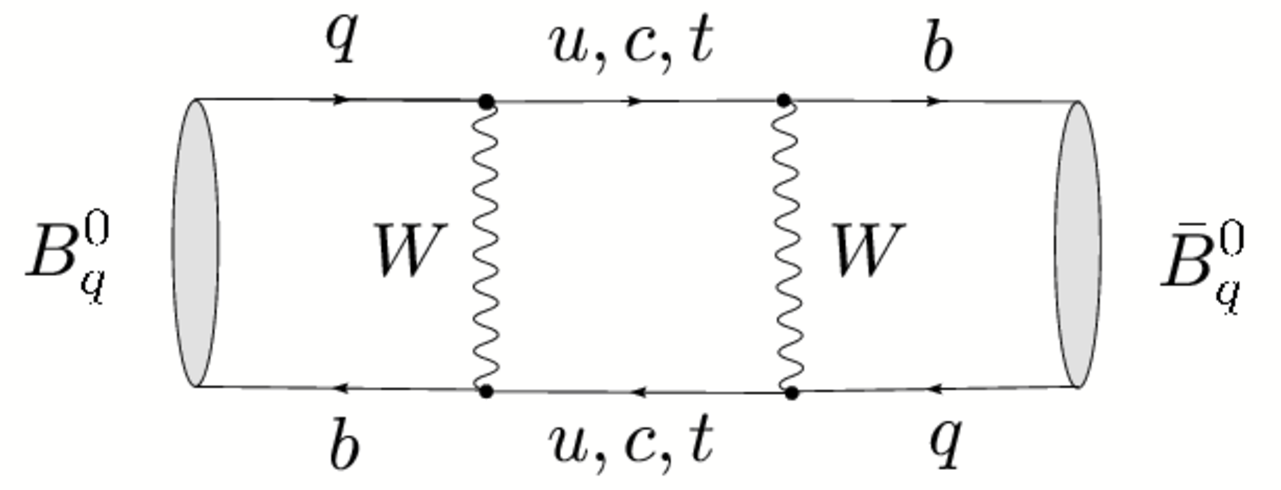
\includegraphics[width=0.5\linewidth]{figures/theory/mixing.pdf}
%\caption{Feynman diagram of mixing between $\Bz_q$ and $\Bzb_q$, where $q$ represents a \dquark or \squark quark.}
%\label{mixing}
%\end{figure}
\begin{figure}[!h]
\centering
	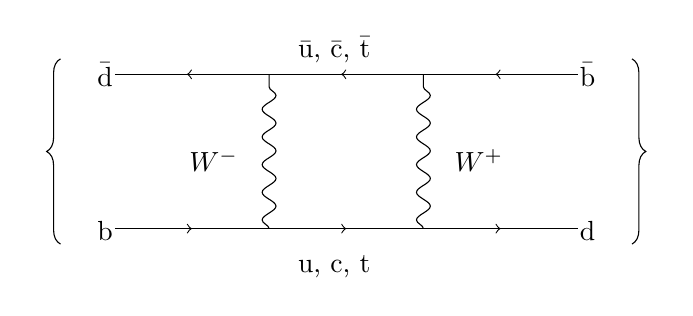
\begin{tikzpicture}[scale=0.98]
        % MAP OUT VERTICES (I have 8 of them)
        \coordinate (a) at (0,3); %b quark start
        \coordinate (b) at (0,1); %ubar quark start
        \coordinate (c) at (6,1); %ubar quark end
        \coordinate (d) at (6,3); %c quark end
        \coordinate (e) at (2,1); %start the W-
        \coordinate (f) at (4,1); %start the W+
        \coordinate (g) at (2,3); %end the W-
        \coordinate (h) at (4,3); %end the W+
        % DRAW LINES
        \draw[antiparticle] (a)  -- (g); %dbar quark
        \draw[antiparticle] (g)  -- (h); %u,c,t bar quark
        \draw[antiparticle] (h)  -- (d); %bbar quark
        \draw[particle] (b)  -- (e); %b quark
        \draw[particle] (e)  -- (f); %u,c,t quark 
        \draw[particle] (f)  -- (c); %d quark 
        \draw[photon] (e) -- (g); %W-
        \draw[photon] (f) -- (h); %W+
        %DRAW LABELS
        \node at ($(a)$) [label={[label distance=-4mm] $\bar{\rm d}$},left] {};
        \node at ($(b)$) [label={[label distance=-4mm] b},left] {};
        \node at ($(c)$) [label={[label distance=-4mm] d},right]{};
        \node at ($(d)$) [label={[label distance=-4mm] $\bar{\rm b}$},right] {};
        \node at ($(e)$) [label={[xshift=20pt,yshift=-25pt] u, c, t},right] {};
        \node at ($(g)$) [label={[xshift=20pt,yshift=-3pt] $\bar{\rm u}$, $\bar{\rm c}$, $\bar{\rm t}$},right] {};
        \node at ($(e)$) [label={[xshift=-20pt,yshift=10pt] $W^-$},above] {};
		\node at ($(f)$) [label={[xshift=20pt,yshift=10pt] $W^+$},above] {};
		
        %ADD BRACES
        \draw
        [black,decorate,decoration={brace,amplitude=5pt},xshift=-20pt,yshift=0pt]
          (0,0.8)  -- (0,3.2) node [black,midway,left=0pt,xshift=-5pt]{$\Bz$};
         \draw 	[black,decorate,decoration={brace,amplitude=5pt},xshift=20pt,yshift=0pt]
          (6,3.2)  -- (6,0.8) node [black,midway,right=0pt,xshift=5pt] {$\Bzb$};
	\end{tikzpicture}
\caption{Feynman diagram of mixing between \Bz and \Bzb.}
\label{mixing}
\end{figure}
\item \textbf{\CP violation from the interference of mixing and decay}: This is best illustrated by an example. A \Bs meson (containing a \bquark quark and \squark antiquark) can decay to a \Dsm\Kp or \Dsp\Km final state. However, this process can also proceed via \decay{\Bs}{\Bsb} mixing, where the \Bsb decays to \Dsm\Kp or \Dsp\Km. These decay paths to the same final state interfere with each other, which results in the third form of \CP violation, illustrated by 
\begin{equation*}
\Gamma\left(\decay{\Bs}{\Dsm\Kp}\right) \neq \Gamma\left(\decay{\Bs}{\decay{\Bsb}{\Dsm\Kp}}\right)
\end{equation*}
\end{itemize} 

Each of these three types of \CP violation can be investigated. This thesis focuses on measurements of direct \CP violation within the Standard Model.

\section{The CKM matrix}

Quarks in the Standard Model can interact via the strong, weak or electromagnetic interactions. The weak interaction couples to a rotation of the flavour eigenstates.
Therefore, the eigenstates that take part in the weak interaction (weak eigenstates) are a mixture of the flavour eigenstates that hadronise to produce the observable meson states. The Cabibbo-Kobayashi-Maskawa (CKM) matrix, $V_{CKM}$, given in \eqn\ref{CKMmatrix}, describes the relationship between the weak eigenstates ($d'$, $s'$, $b'$) and flavour eigenstates (\dquark, \squark, \bquark) of the quarks. 
\begin{equation}
\left(
\begin{array}{c} d' \\ s' \\ b'  \end{array} \right) =
\begin{pmatrix} V_{ud} & V_{us} & V_{ub} \\ V_{cd} & V_{cs} & V_{cb} \\ V_{td} & V_{ts} & V_{tb} \end{pmatrix} \left( 
\begin{array}{c} d \\ s \\ b \end{array} \right) =
V_{CKM} \left( \begin{array}{c} d \\ s \\ b \end{array} \right)
\label{CKMmatrix}
\end{equation}
A given element of this matrix, $V_{ij}$, defines the coupling of a $j \to i$ quark transition. Similarly $V_{ij}^*$ defines the coupling of a $\bar{j} \to \bar{i}$ antiquark transition. By definition the CKM matrix is unitary, i.e. $V_{CKM}V_{CKM}^* = \mathds{1}$, assuming there are only three generations of quarks. The CKM matrix is a complex $3 \times 3$ matrix, which yields 18 parameters. The unitarity requirement, corresponding to nine complex equations, reduces the number of free parameters, and five strong phases can be absorbed into the quark fields as they are not physically observable. This leaves four independent free parameters to describe the CKM matrix: three amplitudes and one phase. This free phase parameter is the source of \CP violation in the SM. 

A standard representation of the CKM matrix uses 3 angles, $\theta_{12}$, $\theta_{23}$ and $\theta_{13}$, and one \CP violating phase, $\delta$, as shown in \eqn\ref{standard}. These angles are defined and labelled in a way which relates to the mixing of two specific generations; couplings between the quark generation $i$ and $j$ vanish if $\theta_{ij} = 0$, and $s_{ij}$ and $c_{ij}$ represent $\sin\theta_{ij}$ and $\cos\theta_{ij}$ respectively.
\begin{equation}
V_{CKM} = \begin{pmatrix} 1 & 0 & 0 \\ 
0 & c_{23} & s_{23} \\ 
0 & -s_{23} & c_{23} \end{pmatrix}
\begin{pmatrix} c_{13} & 0 & s_{13}e^{-i\delta_{13}} \\ 
0 & 1 & 0 \\ 
-s_{13}e^{i\delta_{13}} & 0 & c_{13} \end{pmatrix}
\begin{pmatrix} c_{12} & s_{12} & 0 \\ 
-s_{12} & c_{12} & 0 \\ 
0 & 0 & 1 \end{pmatrix}
\label{standard}
\end{equation}

If the CKM matrix was equivalent to the identity matrix there would be no cross-generation weak interaction of the quarks \eg\ a \uquark quark transition mediated by a W boson could only result in a \dquark, not a \squark or \bquark quark. From empirical determination, the magnitude of the elements in the CKM matrix are~\cite{PDG2016}:
\begin{equation}
| V_{CKM} | = \begin{pmatrix} 0.97434^{+0.00011}_{0.00012} & 0.22506 \pm 0.00050 & 0.00357 \pm 0.00015 \\ 0.22492 \pm 0.00050 & 0.97351 \pm 0.00013 & 0.0411 \pm 0.0013 \\ 0.00875^{+0.00032}_{-0.00033} & 0.0403 \pm 0.0013 & 0.99915 \pm 0.00005 \end{pmatrix} \text{ .}
\end{equation}
It can be seen that quark transitions within the same generation are highly favoured; these are known as Cabibbo-favoured decays. Quark transitions across one generation are suppressed, and the suppression is even stronger across two generations. These are known as Cabibbo-suppressed transitions. 

The structure in the CKM matrix can be illustrated by the Wolfenstein parameterisation, given in \eqn\ref{wolf}, which uses parameters $A$, $\lambda$, $\rho$ and $\eta$. 
\begin{equation}
V_{CKM} = \begin{pmatrix} 1 - \lambda^2/2 & \lambda & A\lambda^3(\rho - i\eta) \\ 
-\lambda & 1 - \lambda^2/2 & A\lambda^2 \\ 
A\lambda^3(1 - \rho - i\eta) & -A\lambda^2 & 1 \end{pmatrix}
\label{wolf} \text{ .}
\end{equation} 
This is an approximation of the standard parameterisation given in \eqn\ref{standard}, expanded in powers of the relatively small parameter $\lambda = \sin\theta_{12} = 0.22$. The other parameters are defined by $A\lambda^2 = s_{23}$ and $A\lambda^3(\rho - i\eta) = s_{13}e^{-i\delta}$. The \CP violation can be determined by measuring $\rho - i\eta$.

\section{The CKM unitarity triangle}

Verifying the unitarity of the CKM matrix is of the utmost importance since non-unitarity is a clear sign of physics Beyond the Standard Model~\cite{CKMtriangle}. The unitarity of the CKM matrix leads to nine unitarity conditions, for example $\Vud\Vubs + \Vcd\Vcbs + \Vtd\Vtbs = 0$, which is the most readily applicable to \B physics. These relations can be represented as a triangle in the complex plane, as shown in \fig\ref{triangle}. The triangle representing the condition $\Vud\Vubs + \Vcd\Vcbs + \Vtd\Vtbs = 0$ is the most interesting as all the quantities are experimentally measurable and are of reasonable relative size. The angles are defined as $\alpha$, $\beta$ and \Pgamma, and the area of the triangle is proportional to the amount of \CP violation in the quark sector of the SM~\cite{CKMtriangle}. 
\begin{figure}
\centering
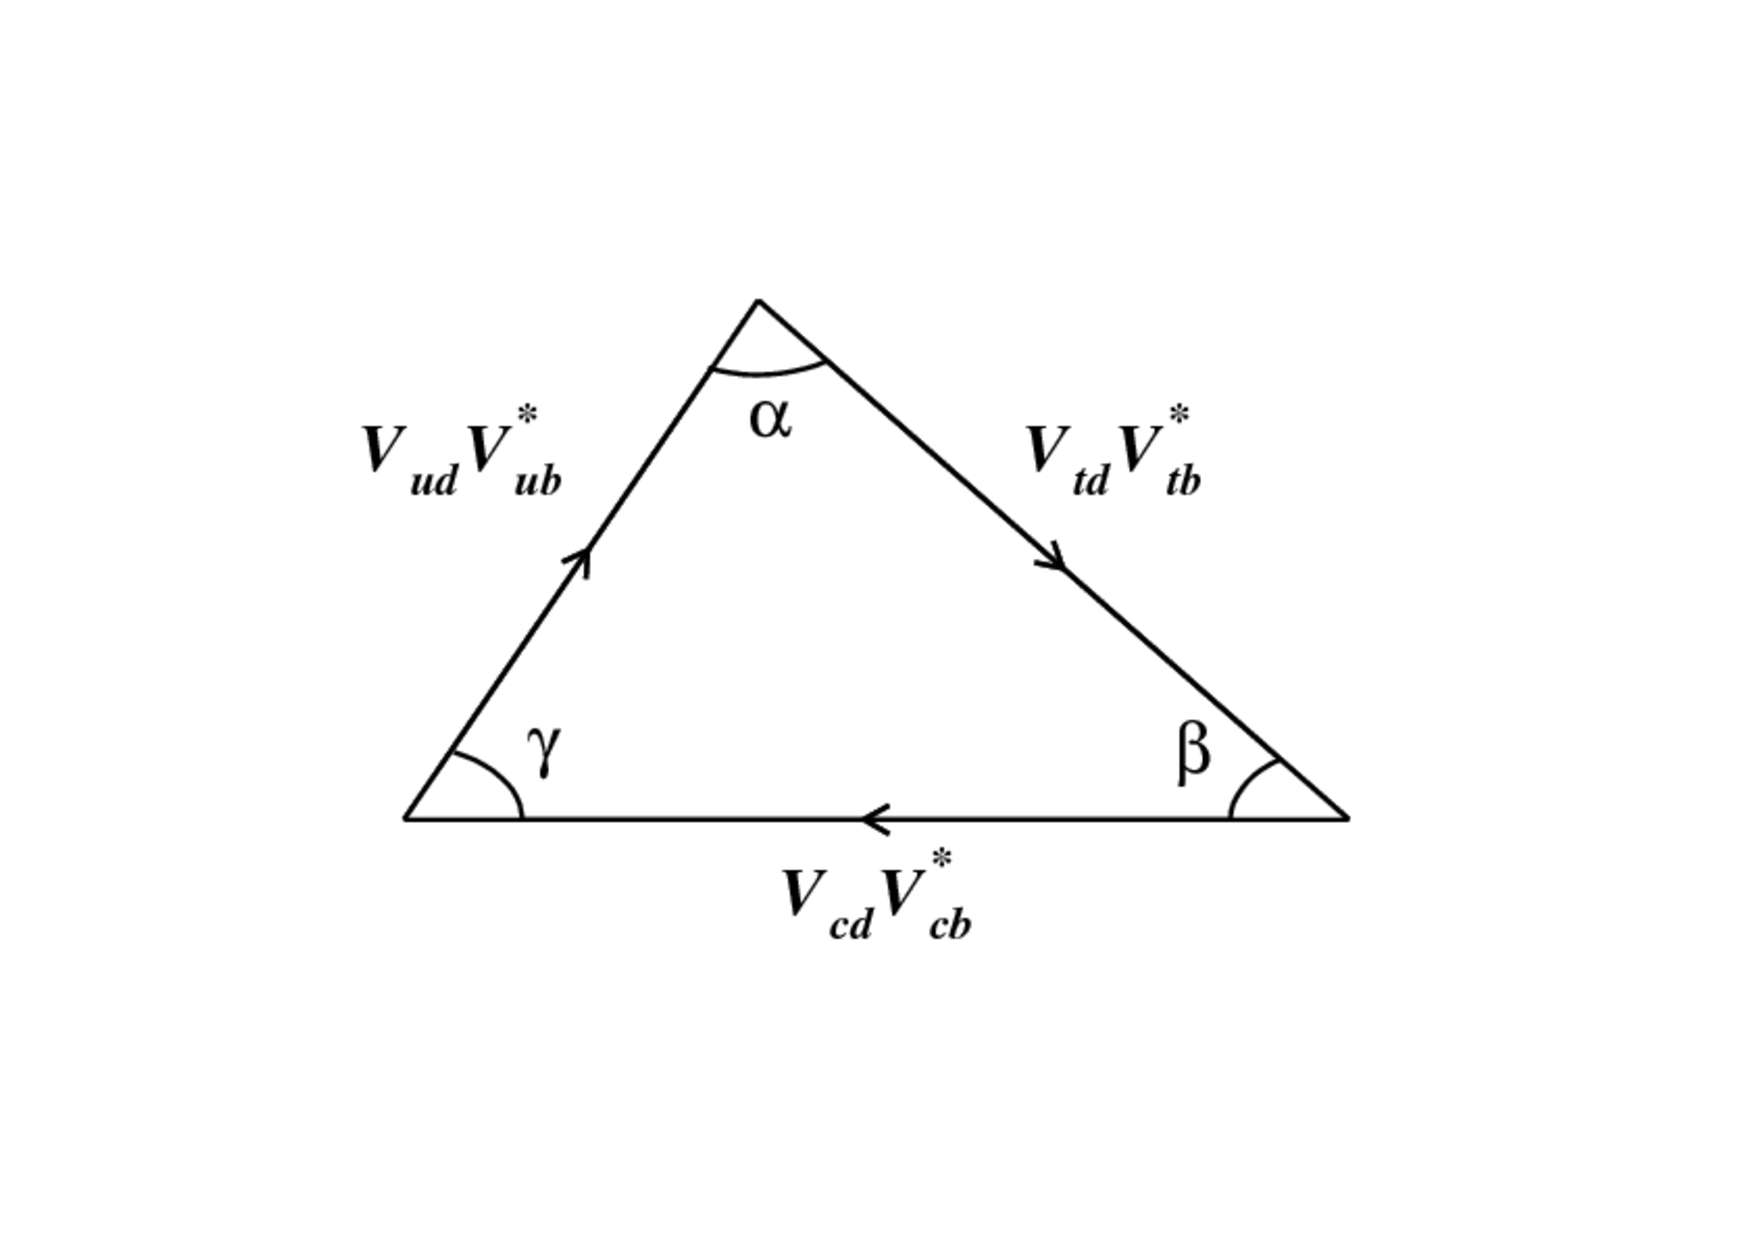
\includegraphics[trim = 50mm 50mm 50mm 50mm,clip,width=0.6\linewidth]{figures/theory/triangle.pdf}
\caption{Graphical representation, in the complex plane, of the unitarity condition $\Vud\Vubs + \Vcd\Vcbs + \Vtd\Vtbs = 0$, forming the CKM triangle with angles $\alpha$, $\beta$ and \Pgamma.}
\label{triangle}
\end{figure}

The values of $\alpha$, $\beta$ and \Pgamma can be accessed by looking at various \B meson decays. The current best measurements for these values are $\alpha = \left(87.6^{+3.5}_{-3.3}\right)^{\circ}$, $\beta = 21.85^{+0.68}_{-0.67}$ and $\Pgamma = \left(72.2^{+6.8}_{-7.3}\right)^{\circ}$~\cite{PDG2016,LHCb-PAPER-2016-032}. Overconstraining this unitarity triangle allows verification as to whether or not the triangle closes, i.e. whether it truly is a triangle. Obtaining inconsistent results from overconstraining would suggest that the CKM matrix is not unitary, which would be incompatible with the SM. 

The CKM angle $\Pgamma \equiv \arg\left(-\frac{\Vud{\Vub}^*}{\Vcd{\Vcb}^*}\right)$ is the angle with the largest uncertainty. This angle is measured using the \lhcb detector from the rates of charged and neutral \B decays to a \D meson (reconstructed in one of a variety of final states) and kaons or pions. These are known as direct measurements. In order to obtain the most precise direct measurement of \Pgamma, the individual measurements from each of these \Pgamma-sensitive decays are combined to produce a single value with a lower uncertainty. The latest published \lhcb combination is $\Pgamma = \left(72.2^{+6.8}_{-7.3}\right)^{\circ}$~\cite{LHCb-PAPER-2016-032}. This is the most precise determination of \Pgamma from direct measurements from a single experiment; other experiments are consistent, but less precise~\cite{Babar_gamma,Belle_gamma}. These measurements involve only tree level process, making them theoretically clean. New particles that are not predicted in the SM can only contribute at higher order, and are therefore highly suppressed.

A global fit to the CKM triangle from CKMfitter~\cite{CKMFitter}, shown in \fig\ref{globalfit}, uses the current best measurements of various quantities, such as $\beta$, $\Delta m_d$ and $\Delta m_s$, as inputs, where $\Delta m_d$ and $\Delta m_s$ are the mass differences between the mass eigenstates of \Bz-\Bzb and \Bs-\Bsb respectively. When performing this fit any information on \Pgamma from direct measurements can be ignored. Assuming the SM, i.e. unitarity of CKM matrix, \Pgamma can be extracted from the global fit. This is known as an indirect measurement. The measurements for the inputs used include loop processes. The presence of loops in the corresponding Feynman diagrams allows additional Beyond the Standard Model diagrams, where new particles appear in the loop contributing to the amplitude at the same order. Therefore, these loop processes, and by extension the extracted indirect measurement of \Pgamma, are sensitive to New Physics. This method obtains a \Pgamma measurement of $(65.3^{+1.0}_{-2.5})^{\circ}$, where this determination of \Pgamma excludes all direct measurements and assumes the SM. The leading theoretical uncertainties on the indirect measurement are from lattice QCD, therefore these uncertainties are expected to decrease as lattice QCD calculations become more accurate. 
\begin{figure}[!ht]
\centering
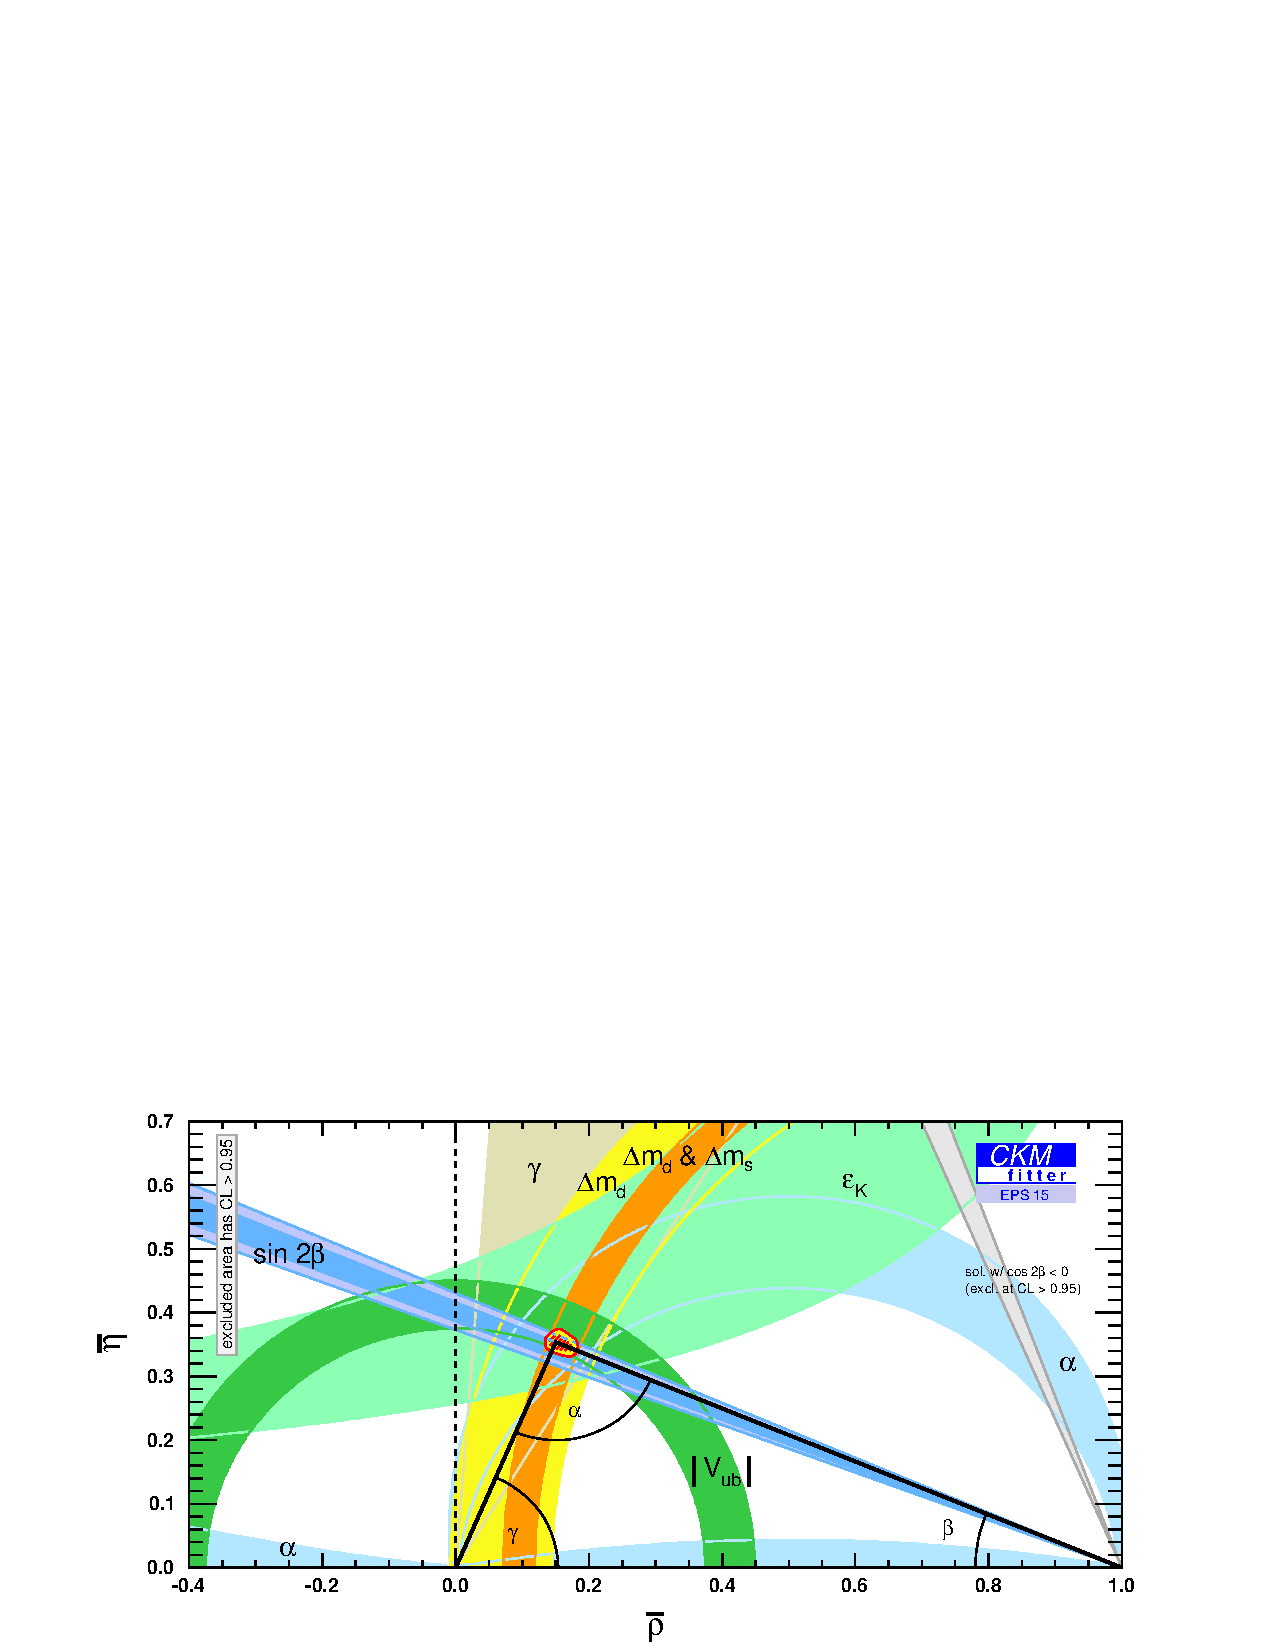
\includegraphics[trim = 0mm 0mm 0mm 180mm,clip,width=0.9\linewidth]{figures/theory/rhoeta_small_global.pdf}
\caption{Diagram showing the current state of measurements of the unitarity triangle~\cite{CKMFitter}. The black line shows the best fit obtained by CKMfitter. The axes $\bar{\rho}$ and $\bar{\eta}$ are the normalised versions of the $\rho$ and $\eta$ parameters in the Wolfenstein parameterisation of the CKM matrix, shown in \eqn\ref{wolf}.}
\label{globalfit}
\end{figure}

The direct and indirect measurements of \Pgamma are currently consistent with each other, however, the result of \Pgamma from direct measurements has a relatively large uncertainty and higher central value. Therefore, improving the precision of the direct measurement of \Pgamma is necessary to verify whether or not the direct and indirect measurements are consistent, thereby testing the consistency of the SM. Improvements in the precision can be achieved through a combination of methods and measurements of various \B decays that are sensitive to \Pgamma; those relevant to this thesis are outlined below.

\section{Tree-level determination of \Pgamma using \decay{\Bpm}{\D K^{(*)\pm}} decays}
\label{sec:theory:gamma}

Direct measurements of \Pgamma can be made by exploiting the interference between \decay{\bquark}{\cquark\uquarkbar\squark} and \decay{\bquark}{\uquark\cquarkbar\squark} transitions. These transitions are present at tree-level in $\Bpm \to \D\kaon^{*\pm}$ decays, represented by the Feynman diagrams shown in \fig\ref{fig:B2DKstarmdiagram}, showing the \decay{\Bm}{\Dz\Kstarm} decay (left) and the \decay{\Bm}{\Dzb\Kstarm} decay (right). Here, as previously mentioned, \D represents the superposition of \Dz and \Dzb mesons. The branching
fraction is of similar order to \decay{\Bm}{\Dzb\Km} which has been extensively analysed~\cite{LHCb-PAPER-2016-003,LHCb-PAPER-2014-041,LHCb-PAPER-2015-014}.
\begin{figure}[!h]
\centering
\resizebox{0.48\linewidth}{!}{
	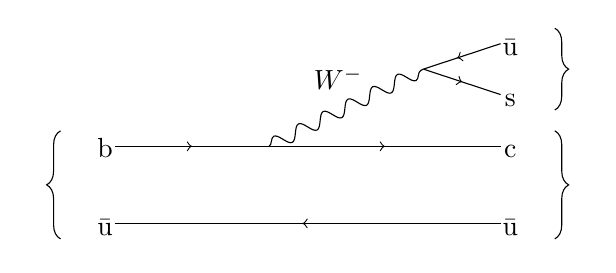
\begin{tikzpicture}[scale=0.98]
        % MAP OUT VERTICES (I have 8 of them)
        \coordinate (a) at (0,2); %b quark start
        \coordinate (b) at (0,1); %ubar quark start
        \coordinate (c) at (5,1); %ubar quark end
        \coordinate (d) at (5,2); %c quark end
        \coordinate (e) at (2,2); %start the W+
        \coordinate (f) at (5,2.67); %s quark
        \coordinate (g) at (5,3.33); %ubar quark
        \coordinate (h) at (4.0,3); %W end
        % DRAW LINES
        \draw[antiparticle] (b)  -- (c); %ubar quark
        \draw[particle] (a)  -- (e); %bbar quark
        \draw[particle] (e)  -- (d); %ubar quark 
        \draw[photon] (e) -- (h); %W+
        \draw[antiparticle] (h)  to (g); %W to ubar quark
        \draw[particle] (h)  to (f); %W to s quark 
        %DRAW LABELS
        \node at ($(a)$) [label={[label distance=-4mm] b},left] {};
        \node at ($(b)$) [label={[label distance=-4mm] $\bar{\rm u}$},left] {};
        \node at ($(c)$) [label={[label distance=-4mm] $\bar{\rm u}$},right]{};
        \node at ($(d)$) [label={[label distance=-4mm] c},right] {};
        \node at ($(f)$) [label={[label distance=-4mm] s},right] {};
        \node at ($(g)$) [label={[label distance=-4mm] $\bar{\rm u}$},right]{};
        \node at ($(e)$) [label={[xshift=25pt,yshift=10pt] $W^-$},above] {};

        %ADD BRACES
        \draw
        [black,decorate,decoration={brace,amplitude=5pt},xshift=-20pt,yshift=0pt]
          (0,0.8)  -- (0,2.2) node [black,midway,left=0pt,xshift=-5pt]{$\Bm$};
        \draw
        [black,decorate,decoration={brace,amplitude=5pt},xshift=20pt,yshift=0pt]
          (5,3.53) -- (5,2.47) node [black,midway,right=0pt,xshift=5pt]{$\Kstarm$};
         \draw 	[black,decorate,decoration={brace,amplitude=5pt},xshift=20pt,yshift=0pt]
          (5,2.2)  -- (5,0.8) node [black,midway,right=0pt,xshift=5pt] {$\Dz$};
            \end{tikzpicture}
        }
\resizebox{0.47\linewidth}{!}{
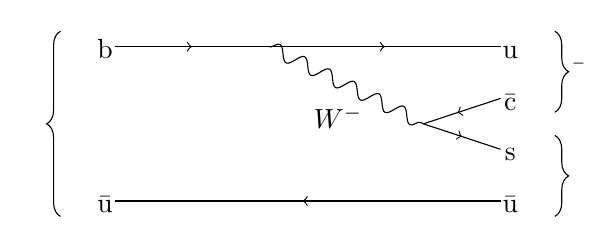
\begin{tikzpicture}[scale=0.98]
        % MAP OUT VERTICES (I have 8 of them)
        \coordinate (a) at (0,3); %b quark start
        \coordinate (b) at (0,1); %ubar quark start
        \coordinate (c) at (5,1); %ubar quark end
        \coordinate (d) at (5,3); %u quark end
        \coordinate (e) at (2,3); %start the W+
        \coordinate (f) at (5,1.67); %s quark
        \coordinate (g) at (5,2.33); %cbar quark
        \coordinate (h) at (4.0,2); %W end
        % DRAW LINES
        \draw[antiparticle] (b)  -- (c); %ubar quark
        \draw[particle] (a)  -- (e); %b quark
        \draw[particle] (e)  -- (d); %u quark 
        \draw[photon] (e) -- (h); %W+
        \draw[antiparticle] (h)  to (g); %W to cbar quark
        \draw[particle] (h)  to (f); %W to s quark 
        %DRAW LABELS
        \node at ($(a)$) [label={[label distance=-4mm] b},left] {};
        \node at ($(b)$) [label={[label distance=-4mm] $\bar{\rm u}$},left] {};
        \node at ($(c)$) [label={[label distance=-4mm] $\bar{\rm u}$},right]{};
        \node at ($(d)$) [label={[label distance=-4mm] u},right] {};
        \node at ($(f)$) [label={[label distance=-4mm] s},right] {};
        \node at ($(g)$) [label={[label distance=-4mm] $\bar{\rm c}$},right]{};
        \node at ($(e)$) [label={[xshift=25pt,yshift=-40pt] $W^-$},above] {};

        %ADD BRACES
        \draw 	[black,decorate,decoration={brace,amplitude=5pt},xshift=-20pt,yshift=0pt]
        (0,0.8)  -- (0,3.2) node [black,midway,left=0pt,xshift=-5pt] {$\Bm$};
        \draw [black,decorate,decoration={brace,amplitude=5pt},xshift=20pt,yshift=0pt]
        (5,1.85)  -- (5,0.8) node [black,midway,right=0pt,xshift=5pt] {$\Kstarm$};
         \draw [black,decorate,decoration={brace,amplitude=5pt},xshift=20pt,yshift=0pt]
        (5,3.2)  -- (5,2.15) node [black,midway,right=0pt,xshift=5pt] {$\bar{\rm \Dz}$};
        \end{tikzpicture}
    }
    \caption{Leading order Feynman diagrams for \decay{\Bm}{\Dz\Kstarm} (left) and \decay{\Bm}{\Dzb\Kstarm} (right).}
    \label{fig:B2DKstarmdiagram}
\end{figure}

The ratio of the amplitudes between the \decay{\Bm}{\Dzb\Kstarm} decay and the \decay{\Bm}{\Dz\Kstarm} decay, and their charge conjugates are given by,
\begin{equation}
\frac{\mathcal{A}\left(\decay{\Bm}{\Dzb\Kstarm}\right)}{\mathcal{A}\left(\decay{\Bm}{\Dz\Kstarm}\right)} = \rb^{DK^*} e^{i(\deltab^{DK^*} - \gamma)} \text{ , }
\frac{\mathcal{A}\left(\decay{\Bp}{\Dz\Kstarp}\right)}{\mathcal{A}\left(\decay{\Bp}{\Dzb\Kstarp}\right)} = \rb^{DK^*} e^{i(\deltab^{DK^*} + \gamma)} \text{ .}
\label{ratiodiagrams}
\end{equation}
There are three parameters in \eqn\ref{ratiodiagrams}: $\rb^{DK^*}$, $\deltab^{DK^*}$ and \Pgamma. Here $\rb^{DK^*}$ is the magnitude of the ratio of the amplitudes and $\deltab^{DK^*}$ is difference in strong phase between the \decay{\Bm}{\Dz\Kstarm} and \decay{\Bm}{\Dzb\Kstarm} decays. When the \D meson is reconstructed in a final state accessible to both \Dz and \Dzb meson states, $f(D)$, interference occurs, as shown in \fig\ref{paths}. This interference gives sensitivity to the weak phase \Pgamma.

\begin{figure}
\centering
%\includegraphics[trim = 20mm 120mm 100mm 20mm,clip,width=0.7\linewidth]{figures/theory/test.pdf}
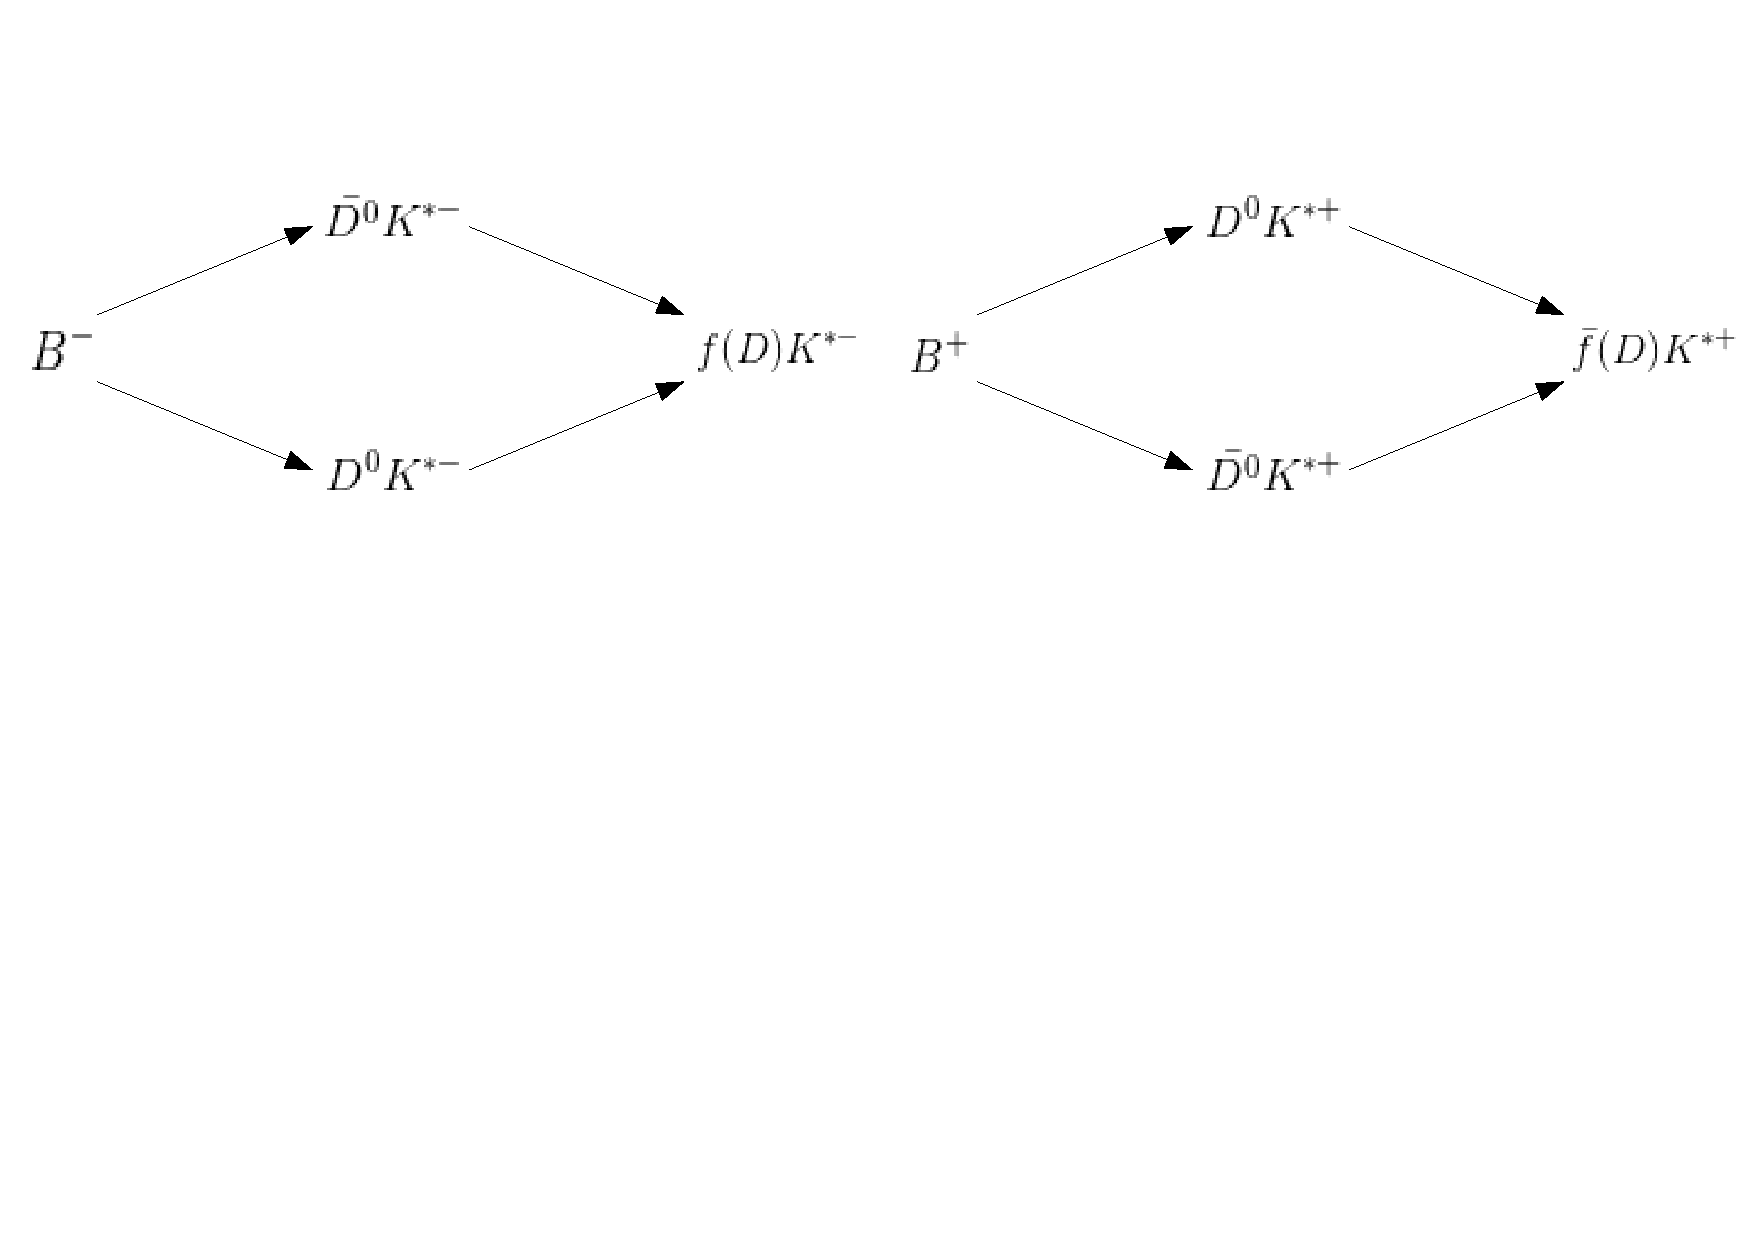
\includegraphics[trim = 0mm 120mm 0mm 30mm,clip,width=\linewidth]{figures/theory/pathDiagrams.pdf}
\put(-425,75) {\small $\rb^{DK^*} e^{i(\deltab^{DK^*} - \gamma)}$}
\put(-215,75) {\small $\rb^{DK^*} e^{i(\deltab^{DK^*} + \gamma)}$}
\put(-285,70) {\small $\bar{A_{D}}$}
\put(-285,12) {\small $A_D$}
\put(-75,70) {\small $A_D$}
\put(-75,12) {\small $\bar{A_{D}}$}
\caption{Diagram of the interfering amplitudes of \decay{\Bm}{\D\Kstarm} (left) and \decay{\Bp}{\D\Kstarp} (right), where $A_D$ is the amplitude of \decay{\Dz}{f(D)} and $\bar{A_{D}}$ is the amplitude of \decay{\Dzb}{f(D)}.}
\label{paths}
\end{figure}

In the following description we assume \CP violation in the charm sector is negligible, and effects of \D mixing are neglected~\cite{charmcpv,charmmixing}. The partial widths for the \Bm and \Bp decays are given by \eqns\ref{pwminus} and \ref{pwplus}, where $A_D$ is the amplitude of \decay{\Dz}{f(D)} and $\bar{A_{D}}$ is the amplitude of \decay{\Dzb}{f(D)}.
\begin{align}
\Gamma\left(\decay{\Bm}{[f(D)]\Kstarm}\right) &\propto |A_D|^2 + (\rb^{DK^*})^2 |\bar{A_{D}}|^2 + 2\rb^{DK^*} Re\left[ A_D \bar{A_{D}} e^{-i(\deltab^{DK^*} - \gamma)} \right] \label{pwminus} \\
\Gamma\left(\decay{\Bp}{[f(D)]\Kstarp}\right) &\propto |A_D|^2 + (\rb^{DK^*})^2 |\bar{A_{D}}|^2 + 2\rb^{DK^*} Re\left[ A_D \bar{A_{D}} e^{-i(\deltab^{DK^*} + \gamma)} \right] \label{pwplus}
\end{align}

The values of the complex amplitudes, $A_{D}$ and $\bar{A_{D}}$, depend on the \D meson final state chosen. The sensitivity to \Pgamma can therefore be maximised by a judicious choice of \Dz decay mode, through the dependencies of $A_{D}$ and $\bar{A_{D}}$.

\subsection{The GLW and quasi-GLW methods}
\label{sec:theory:glw}

The theorists Gronau, London and Wyler proposed the study of \decay{\Bm}{\D\Km} modes with the \D decays into a \CP eigenstate, referred to as the GLW method~\cite{GL,GW}, such as the eigenstates \decay{\Dz}{\Kp\Km} and \decay{\Dz}{\pip\pim}. A \CP eigenstate is a state which is preserved under a \CP transformation. As these final states are \CP-even, $A_{D} = \bar{A_{D}}$, and hence the expressions from \eqns\ref{pwminus} and \ref{pwplus} can be simplified to
\begin{align}
\Gamma\left(\decay{\Bm}{[f_{GLW}]\Kstarm}\right) &\propto 1 + (\rb^{DK^*})^2 + 2\rb^{DK^*}\cos(\deltab^{DK^*} - \gamma) \label{widthBm} \\
\Gamma\left(\decay{\Bp}{[f_{GLW}]\Kstarp}\right) &\propto 1 + (\rb^{DK^*})^2 + 2\rb^{DK^*}\cos(\deltab^{DK^*} + \gamma) \text { ,}\label{widthBp}
\end{align}
assuming that \CP violation in \D decays is negligible and $\mathcal{A}\left(\decay{\Bm}{\Dz\Kstarm}\right) = \mathcal{A}\left(\decay{\Bp}{\Dzb\Kstarp}\right)$. 

The four-body \D decay mode \decay{\D}{\pip\pim\pip\pim} is a self-conjugate decay mode, containing a mixture of \CP-even and \CP-odd states, which can be used to measure \Pgamma via the GLW method provided the fractional \CP-even content is known~\cite{NAYAK20151}. As this mode is not a pure \CP eigenstate, it is referred to as a quasi-GLW (qGLW) mode, and its sensitivity to \Pgamma is reduced. The \CP-even fraction, $F_{4\pi}$, measured to be $0.737 \pm 0.028$~\cite{charm4pi}, accounts for the dilution effect. The partial widths for this self-conjugate qGLW mode~\cite{NAYAK20151,charm4pi}, corresponding to \eqns\ref{widthBm} and \ref{widthBp}, are
\begin{align}
\Gamma\left(\decay{\Bm}{[f_{qGLW}]\Kstarm}\right) \propto 1 + (\rb^{DK^*})^2 + 2\rb^{DK^*}\left(2F_{4\pi} - 1\right)\cos(\deltab^{DK^*} - \gamma) \label{widthBm4body} \\
\Gamma\left(\decay{\Bp}{[f_{GLW}]\Kstarp}\right) \propto 1 + (\rb^{DK^*})^2 + 2\rb^{DK^*}\left(2F_{4\pi} - 1\right)\cos(\deltab^{DK^*} + \gamma) \text { .} \label{widthBp4body}
\end{align}
In \eqns\ref{widthBm4body} and \ref{widthBp4body}, it can be seen that the expression $2F_{4\pi} - 1$ modulates the \Pgamma-sensitive interference term.


\subsection{The ADS method}
\label{sec:theory:ads}

The theorists Atwood, Dunietz and Soni proposed looking at \D decay modes where $f(D)$ is a non-\CP eigenstate, \eg~\decay{\D}{\Km\pip}, referred to as the ADS method~\cite{ADS,ADS-2001}. A key feature of this method is that although the \Dz and \Dzb decay to the same final state, they proceed by very different amplitudes. The Feynman diagrams for the doubly Cabibbo-favoured \decay{\Dz}{\Km\pip} decay and the doubly Cabibbo-suppressed \decay{\Dz}{\Kp\pim} decay are shown in \fig\ref{fig:D2KPidiagram}.
\begin{figure}[!h]
\centering
\resizebox{0.48\linewidth}{!}{
	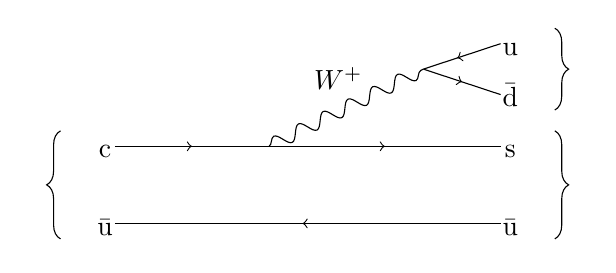
\begin{tikzpicture}[scale=0.98]
        % MAP OUT VERTICES (I have 8 of them)
        \coordinate (a) at (0,2); %c quark start
        \coordinate (b) at (0,1); %ubar quark start
        \coordinate (c) at (5,1); %ubar quark end
        \coordinate (d) at (5,2); %s quark end
        \coordinate (e) at (2,2); %start the W+
        \coordinate (f) at (5,2.67); %dbar quark
        \coordinate (g) at (5,3.33); %u quark
        \coordinate (h) at (4.0,3); %W end
        % DRAW LINES
        \draw[antiparticle] (b)  -- (c); %ubar quark
        \draw[particle] (a)  -- (e); %bbar quark
        \draw[particle] (e)  -- (d); %ubar quark 
        \draw[photon] (e) -- (h); %W+
        \draw[antiparticle] (h)  to (g); %W to ubar quark
        \draw[particle] (h)  to (f); %W to s quark 
        %DRAW LABELS
        \node at ($(a)$) [label={[label distance=-4mm] c},left] {};
        \node at ($(b)$) [label={[label distance=-4mm] $\bar{\rm u}$},left] {};
        \node at ($(c)$) [label={[label distance=-4mm] $\bar{\rm u}$},right]{};
        \node at ($(d)$) [label={[label distance=-4mm] s},right] {};
        \node at ($(f)$) [label={[label distance=-4mm] $\bar{\rm d}$},right]{};
        \node at ($(g)$) [label={[label distance=-4mm] u},right]{};
        \node at ($(e)$) [label={[xshift=25pt,yshift=10pt] $W^+$},above] {};

        %ADD BRACES
        \draw
        [black,decorate,decoration={brace,amplitude=5pt},xshift=-20pt,yshift=0pt]
          (0,0.8)  -- (0,2.2) node [black,midway,left=0pt,xshift=-5pt]{\Dz};
        \draw
        [black,decorate,decoration={brace,amplitude=5pt},xshift=20pt,yshift=0pt]
          (5,3.53) -- (5,2.47) node [black,midway,right=0pt,xshift=5pt]{\pip};
         \draw 	[black,decorate,decoration={brace,amplitude=5pt},xshift=20pt,yshift=0pt]
          (5,2.2)  -- (5,0.8) node [black,midway,right=0pt,xshift=5pt] {\Km};
            \end{tikzpicture}
        }
\resizebox{0.47\linewidth}{!}{
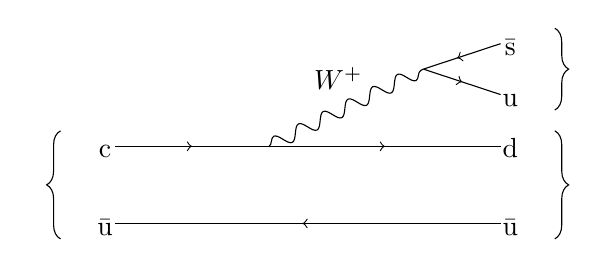
\begin{tikzpicture}[scale=0.98]
        % MAP OUT VERTICES (I have 8 of them)
        \coordinate (a) at (0,2); %c quark start
        \coordinate (b) at (0,1); %ubar quark start
        \coordinate (c) at (5,1); %ubar quark end
        \coordinate (d) at (5,2); %d quark end
        \coordinate (e) at (2,2); %start the W+
        \coordinate (f) at (5,2.67); %u quark
        \coordinate (g) at (5,3.33); %sbar quark
        \coordinate (h) at (4.0,3); %W end
        % DRAW LINES
        \draw[antiparticle] (b)  -- (c); %ubar quark
        \draw[particle] (a)  -- (e); %bbar quark
        \draw[particle] (e)  -- (d); %ubar quark 
        \draw[photon] (e) -- (h); %W+
        \draw[antiparticle] (h)  to (g); %W to ubar quark
        \draw[particle] (h)  to (f); %W to s quark 
        %DRAW LABELS
        \node at ($(a)$) [label={[label distance=-4mm] c},left] {};
        \node at ($(b)$) [label={[label distance=-4mm] $\bar{\rm u}$},left] {};
        \node at ($(c)$) [label={[label distance=-4mm] $\bar{\rm u}$},right]{};
        \node at ($(d)$) [label={[label distance=-4mm] d},right]{};
        \node at ($(f)$) [label={[label distance=-4mm] u},right]{};
        \node at ($(g)$) [label={[label distance=-4mm] $\bar{\rm s}$},right]{};
        \node at ($(e)$) [label={[xshift=25pt,yshift=10pt] $W^+$},above] {};

        %ADD BRACES
        \draw
        [black,decorate,decoration={brace,amplitude=5pt},xshift=-20pt,yshift=0pt]
          (0,0.8)  -- (0,2.2) node [black,midway,left=0pt,xshift=-5pt]{\Dz};
        \draw
        [black,decorate,decoration={brace,amplitude=5pt},xshift=20pt,yshift=0pt]
          (5,3.53) -- (5,2.47) node [black,midway,right=0pt,xshift=5pt]{\Kp};
         \draw 	[black,decorate,decoration={brace,amplitude=5pt},xshift=20pt,yshift=0pt]
          (5,2.2)  -- (5,0.8) node [black,midway,right=0pt,xshift=5pt] {\pim};
            \end{tikzpicture}
    }
    \caption{Leading order Feynman diagrams for \decay{\Dz}{\Km\pip} (left) and \decay{\Dz}{\Kp\pim} (right).}
    \label{fig:D2KPidiagram}
\end{figure}

The ratio of the amplitudes of \decay{\Dzb}{\Km\pip} and \decay{\Dz}{\Km\pip} is given by\footnote{The \CP operator acting on the state $\ket{\Dz}$ can result in either $\CP\ket{\Dz} = \ket{\Dzb}$ or $\CP\ket{\Dz} = - \ket{\Dzb}$. This has consequences for the definition of the strong phase difference. In the ADS formalism, which is used here, the definition $\CP\ket{\Dz} = \ket{\Dzb}$ is used, resulting in \eqn\ref{ratioads}. The alternative definition, $\CP\ket{\Dz} = - \ket{\Dzb}$, used by HFLAV and in the CLEO-c analysis in Ref~\cite{charmkpi_deltab}, would result in $r_D^{K\pi}e^{-i(\pi + \delta_D^{K\pi})}$. The consequence of this is that the measured value of the strong phase difference taken from Ref.~\cite{charmkpi_deltab} must be offset by $180^{\circ}$ when used in the analysis presented in this thesis.}
\begin{equation}
\frac{\mathcal{A}\left(\decay{\Dzb}{\Km\pip}\right)}{\mathcal{A}\left(\decay{\Dz}{\Km\pip}\right)} = r_D^{K\pi}e^{-i\delta_D^{K\pi}} \text { ,}
\label{ratioads}
\end{equation}
where the parameter $r_D^{K\pi}$ is the magnitude of the ratio of amplitudes and $\delta_D^{K\pi}$ is the difference in strong phase between the suppressed and favoured decays. These parameters have been previously measured to be $r_D^{K\pi} = 0.0591 \pm 0.0003$ and $\delta_D^{K\pi} = \left(191.8 \pm 12.1\right)^{\circ}$~\cite{HFAG}.

\Eqn\ref{ratioads} can be expressed as $\bar{A_{D}}/A_{D} = r_D^{K\pi}e^{-i\delta_D^{K\pi}}$ for the case where $f(D)$ is \Km\pip, and similarly, $A_{D}/\bar{A_{D}} = r_D^{K\pi}e^{-i\delta_D^{K\pi}}$ for the case where $f(D)$ is \Kp\pim. Using these expressions, the partial widths from \eqns\ref{pwminus} and \ref{pwplus} for the various \decay{\Bpm}{\D\Kstarpm} ADS decay modes are given by
\begin{align}
\Gamma\left(\decay{\Bm}{[\Kp\pim]\Kstarm}\right) &\propto (\rb^{DK^*})^2 + (r_D^{K\pi})^2 + 2\rb^{DK^*}r_D^{K\pi}\cos(\deltab^{DK^*} + \delta_D^{K\pi} - \gamma) \label{adsBdecaym} \\
\Gamma\left(\decay{\Bp}{[\Km\pip]\Kstarp}\right) &\propto (\rb^{DK^*})^2 + (r_D^{K\pi})^2 + 2\rb^{DK^*}r_D^{K\pi}\cos(\deltab^{DK^*} + \delta_D^{K\pi} + \gamma) \label{adsBdecayp} \\
\Gamma\left(\decay{\Bm}{[\Km\pip]\Kstarm}\right) &\propto 1 + (\rb^{DK^*})^2(r_D^{K\pi})^2 + 2\rb^{DK^*}r_D^{K\pi}\cos(\deltab^{DK^*} + \delta_D^{K\pi} + \gamma) \label{favBdecaym} \\
\Gamma\left(\decay{\Bp}{[\Kp\pim]\Kstarp}\right) &\propto 1 + (\rb^{DK^*})^2(r_D^{K\pi})^2 + 2\rb^{DK^*}r_D^{K\pi}\cos(\deltab^{DK^*} + \delta_D^{K\pi} - \gamma) \text {.} \label{favBdecayp} 
\end{align}
For the analysis considered in this thesis, the favoured decay contains a \Kstarm meson and pion from the \D meson of opposite charge, while in the suppressed decay the \Kstarm meson and the pion from the \D meson have the same charge. The ADS decay mode is a combination of a CKM-favoured \decay{\Bm}{\Dz\Kstarm} decay (\fig\ref{fig:B2DKstarmdiagram}, left), followed by a doubly Cabibbo-suppressed \decay{\Dz}{\Kp\pim} decay (\fig\ref{fig:D2KPidiagram}, right), and a CKM- and colour-suppressed \decay{\Bm}{\Dzb\Kstarm} decay (\fig\ref{fig:B2DKstarmdiagram}, right), followed by a Cabibbo-favoured \decay{\Dzb}{\Kp\pim} decay (\fig\ref{fig:D2KPidiagram}, left). Both paths to the same final state have amplitudes of similar size, and interference effects are therefore magnified in comparison to the GLW decay modes, where the decay path via the CKM-favoured \decay{\Bm}{\Dz\Kstarm} decay dominates.

Two-body \decay{\D}{\Kmp\pipm} decays are characterised by two parameters, an amplitude ratio and a single strong phase, as illustrated in \eqn\ref{ratioads}. However for multibody \decay{\D}{\Kmp\pipm\pimp\pipm} decays, the strong phase varies over the phase space. Therefore, the amplitude at each point in phase space, $p$, must be considered for both the \decay{\Dz}{\Km\pip\pim\pip} favoured and \decay{\Dz}{\Kp\pim\pip\pim} suppressed decays, referred to as $A_{fav}(p)$ and $A_{sup}(p)$ respectively. The three hadronic parameters that describe the \decay{\D}{\Km\pip\pim\pip} decay~\cite{charmk3pi,charmk3pi_errata,LHCb-PAPER-2015-057} are defined by
\begin{align}
r_D^{K3\pi} &= \frac{\int \mathrm{d}p \left|A_{sup}(p)\right|^2}{\int \mathrm{d}p \left|A_{fav}(p)\right|^2}
\label{rddefinition}
\end{align}
and
\begin{align}
R_{K3\pi} e^{i\delta_D^{K3\pi}} &= \frac{\int \mathrm{d}p A_{fav}(p)A_{sup}(p)}{\sqrt{\int \mathrm{d}p \left|A_{fav}(p)\right|^2 \int \mathrm{d}p \left|A_{sup}(p)\right|^2}} \text { ,}
\label{Rddefinition}
\end{align}
where $r_D^{K3\pi}$ is the amplitude ratio between suppressed and favoured \decay{\D}{\Km\pip\pim\pip} decays (analogous to $r_D^{K\pi}$), $R_{K3\pi}$ is a coherence factor to account for the dilution of the interference effects due to averaging over phase space, and $\delta_D^{K3\pi}$ is the strong phase difference (analogous to $\delta_D^{K\pi}$). These parameters have been measured to be $r_D^{K3\pi} = 0.0549 \pm 0.0006$, $R_{K3\pi} = 0.43 \pm 0.17$ and $\delta_D^{K3\pi} = \left(128 \pm 28\right){\circ}$~\cite{charmk3pi,charmk3pi_errata,LHCb-PAPER-2015-057}. Based on the definitions in \eqns\ref{rddefinition} and \ref{Rddefinition}, the partial widths are given by
\begin{align}
\Gamma\left(\decay{\Bm}{[\Kp\pim]\Kstarm}\right) &\propto (\rb^{DK^*})^2 + (r_D^{K3\pi})^2 + 2\rb^{DK^*}R_{K3\pi}r_D^{K3\pi}\cos(\deltab^{DK^*} + \delta_D^{K3\pi} - \gamma) \label{adsBdecaym4body} \\
\Gamma\left(\decay{\Bp}{[\Km\pip]\Kstarp}\right) &\propto (\rb^{DK^*})^2 + (r_D^{K3\pi})^2 + 2\rb^{DK^*}R_{K3\pi}r_D^{K3\pi}\cos(\deltab^{DK^*} + \delta_D^{K3\pi} + \gamma) \label{adsBdecayp4body} \\
\Gamma\left(\decay{\Bm}{[\Km\pip]\Kstarm}\right) &\propto 1 + (\rb^{DK^*})^2(r_D^{K3\pi})^2 + 2\rb^{DK^*}R_{K3\pi}r_D^{K3\pi}\cos(\deltab^{DK^*} + \delta_D^{K3\pi} + \gamma) \label{favBdecaym4body} \\
\Gamma\left(\decay{\Bp}{[\Kp\pim]\Kstarp}\right) &\propto 1 + (\rb^{DK^*})^2(r_D^{K3\pi})^2 + 2\rb^{DK^*}R_{K3\pi}r_D^{K3\pi}\cos(\deltab^{DK^*} + \delta_D^{K3\pi} - \gamma) \text{ .}\label{favBdecayp4body} 
\end{align}
It can be seen from these equations that the four-body coherence factor, $R_{K3\pi}$, modulates the size of the interference term that carries the dependence on \Pgamma.

\subsection{Physical observables}

This thesis aims to measure \Pgamma as well as the hadronic parameters of \btodkst decays, with the \Kstarm meson decaying to \KS\pim, using the methods and equations discussed in Secs.~\ref{sec:theory:glw} and \ref{sec:theory:ads}. However, experimental considerations must be taken into account when developing the strategy to measure these parameters. For example, the use of the parameters $\rb^{DK^*}$ and $\deltab^{DK^*}$ discussed in \sect\ref{sec:theory:gamma} assumes that a pure sample of \btodkst decays is available. This section introduces the \btodkst coherence factor, $\kappa$, which deals with the contamination from other \decay{\Bm}{\D\KS\pim} processes in order to extract the parameters of interest. This section also describes the experimental quantities that are measured in this analysis in order to gain maximum sensitivity to \Pgamma. 

\subsubsection{Coherence factor}
\label{sec:theory:kappa}

As discussed earlier in this chapter, this thesis considers \decay{\Bm}{\D\Kstarm}, \decay{\Kstarm}{\KS\pim} decays. The \Kstarm meson could be reconstructed in either of the \KS\pim or \Km\piz final states, however, due to the higher reconstruction efficiency of the \KS meson compared to the \piz meson, the \KS\pim final state is pursued. As the \Kstarm meson has a large natural width (about 50~\mevcc~\cite{PDG2016}), it is necessary to consider the effect of other resonant and non-resonant \decay{\Bm}{\D\KS\pim} decays on the experimental measurements of the physics parameters, $\rb^{DK^*}$, $\rb^{DK^*}$ and \Pgamma. The amplitudes and phases of the different decays will vary at each point in \decay{\Bm}{\D\KS\pim} phase space, as given by
\begin{align*}
A(B^- \to D^0 X^-) &= A_c(p) e^{i\delta_c(p)} \\
A(B^- \to \bar{D^0} X^-) &= A_u(p) e^{i(\delta_u(p) - \gamma)} \text{ ,}
\end{align*}
where $p$ is the point in $\left(m^2(\KS\pim),m^2(\D\pim)\right)$ space, where $m^2(\KS\pim) = (p_{\KS} + p_{\pim})^2$, and $m^2(\D\pim) = (p_{\D} + p_{\pim})^2$. Here $p_{X}$ is the four-momentum of particle $X$, the expressions $A_u(p)$ and $A_c(p)$ are the moduli of the \decay{\bquark}{\uquark} and \decay{\bquark}{\cquark} amplitudes respectively, while $\delta_{c}(p)$ and $\delta_{u}(p)$ represent the strong phases of the relevant decay amplitudes. The symbol $X^-$ represents a resonant or non-resonant \KS\pim pair, which could be produced by the decay of the \Kstarm meson or by other contributions to the \decay{\Bm}{\D\KS\pim} final state. The amplitudes of the \Bp decays can be expressed as 
\begin{align*}
A(\decay{\Bp}{\Dzb X^+}) &= A_c(p) e^{i\delta_c(p)} \\
A(\decay{\Bp}{\Dz X^+}) &= A_u(p) e^{i(\delta_u(p) + \gamma)} \text{ .}
\end{align*}
Due to the large natural width of the \Kstarm meson, interference may occur in the region near the \Kstarm mass between the signal \Kstarm decay amplitude and amplitudes due to other \decay{\Bm}{\D\KS\pim} contributions, for example higher \KS\pim resonances and non-resonant decays. The interfering contributions dilute the sensitivity to \Pgamma, which is quantified by the \btodkst coherence factor, $\kappa$, where $0 \leq \kappa \leq 1$, and $\kappa = 1$ denotes a pure $K^{*-}$ contribution giving maximum sensitivity to \Pgamma. The parameters \rb, \deltab and $\kappa$ are then defined for \btodkst decays as
\begin{align}
r_B^2 &= \frac{\Gamma(B^- \to \bar{D^0}X^-)}{\Gamma(B^- \to D^0X^-)} = \frac{\int \left|A_u(p)\right|^2 \mathrm{d}p}{\int \left|A_c(p)\right|^2 \mathrm{d}p}
\label{rbdefinition}
\end{align}
\begin{align}
\kappa e^{i\delta_B} &= \frac{\int \mathrm{d}p A_c(p)A_u(p)e^{i\delta(p)}}{\sqrt{\int \mathrm{d}p \left|A_u(p)\right|^2 \int \mathrm{d}p \left|A_c(p)\right|^2}} \text{ ,}
\label{kappadefinition}
\end{align}
where $p$ represents a point in phase space, $0 \leq \delta(p) \leq 2\pi$, and the integration is performed over a defined \Kstarm region. In \eqns\ref{rbdefinition} and \ref{kappadefinition}, the parameters \rb, \deltab and $\kappa$ depend on the region of the \decay{\Bm}{\D\KS\pim} phase space that is integrated over. In order to maximise sensitivity to \Pgamma an integration region should be chosen that finds the optimal working point between maximising the coherence factor and maximising the size of the data sample available.

As before, it is assumed that \CP violation in the charm sector is negligible, and effects of \D mixing are neglected~\cite{charmcpv,charmmixing}. The partial widths for the \Bm and \Bp decays are then given by \eqns\ref{partialwidthminus} and \ref{partialwidthplus}, where $A_D$ is the amplitude of \decay{\Dz}{f(D)} and $\bar{A_{D}}$ is the amplitude of \decay{\Dzb}{f(D)}.
\begin{align}
\frac{d\Gamma\left(\decay{\Bm}{[f(D)]X^-}\right)}{dp} &\propto | A_c(p) e^{i\delta_c(p)}A_{D} + A_u(p) e^{i(\delta_u(p) - \gamma)}\bar{A_{D}} |^2 \label{partialwidthminus} \\
\frac{d\Gamma\left(\decay{\Bp}{[f(D)]X^-}\right)}{dp} &\propto | A_u(p) e^{i(\delta_u(p) + \gamma)}\bar{A_{D}} + A_c(p) e^{i\delta_c(p)}A_{D} |^2 \label{partialwidthplus}
\end{align}
Expanding and integrating over the defined \Kstar region gives
\begin{align}
\Gamma\left(\decay{\Bm}{[f(D)]X^-}\right) &\propto |A_D|^2 + \rb^2 |\bar{A_{D}}|^2 + 2\kappa\rb Re\left[ A_D \bar{A_{D}} e^{-i(\deltab - \gamma)} \right] \label{BandDdecaysminus} \\
\Gamma\left(\decay{\Bp}{[f(D)]X^-}\right) &\propto |A_D|^2 + \rb^2 |\bar{A_{D}}|^2 + 2\kappa\rb Re\left[ A_D \bar{A_{D}} e^{-i(\deltab + \gamma)} \right] \label{BandDdecaysplus}
\end{align}

A comparison between \eqns\ref{pwminus} and \ref{pwplus} and \eqns\ref{BandDdecaysminus} and \ref{BandDdecaysplus} shows that in order to account for the fact that the \decay{\Bm}{\D\Kstarm} sample contains small contributions from other resonant and non-resonant \decay{\Bm}{\D\KS\pim} decays, the substitutions $(\rb^{DK^*})^2 \to \rb^2$, $\rb^{DK^*} \to \kappa\rb$ and $\deltab^{DK^*} \to \deltab$, are evident. In particular for $\kappa = 1$, \eqns\ref{pwminus} and \ref{pwplus} are recovered. The coherence factor, $\kappa$, that accounts for contributions from other resonant and non-resonant \decay{\Bm}{\D\KS\pim} decays, modulates the size of the interference term that carries the dependence on \Pgamma.

\subsubsection{\CP observables}
\label{sec:theory:observables}

Using the GLW, qGLW and ADS methods, discussed in Secs.~\ref{sec:theory:glw} and \ref{sec:theory:ads}, observable quantities are constructed that can be used to extract \rb, \deltab and \Pgamma. The decay rates for the GLW modes, in \eqns\ref{widthBm} - \ref{widthBp4body}, the two-body ADS modes, in \eqns\ref{adsBdecaym} - \ref{favBdecayp}, and the four-body ADS modes, in \eqns\ref{adsBdecaym4body} - \ref{favBdecayp4body}, can be measured directly by counting the number of observed events. However, by constructing ratios of these decay rates many experimental uncertainties will cancel, thus improving the precision of the results. 

The observables used in this thesis are the asymmetries between the \Bm and \Bp decay rates, as well as ratios of decay rates in comparison to the favoured modes for the different \Dz final states. No \CP asymmetry is expected in the two- and four-body favoured \Dz decay modes. The twelve quantities, collectively referred to as \CP observables, that are measured in this analysis are:

\begin{itemize}
\item{The \CP asymmetry for the favoured decay mode
\begin{equation}
A_{\kaon\pi} = \frac{\Gamma\left(\decay{\Bm}{\D(\Km\pip)\Kstarm}\right) - \Gamma\left(\decay{\Bp}{\D(\Kp\pim)\Kstarp}\right)}{\Gamma\left(\decay{\Bm}{\D(\Km\pip)\Kstarm}\right) + \Gamma\left(\decay{\Bp}{\D(\Kp\pim)\Kstarp}\right)} \text{ .}
\label{eqn:Akpi}
\end{equation}}
\item{The \CP asymmetry for the \decay{\D}{\Kp\Km} decay mode
\begin{equation}
A_{\kaon\kaon} = \frac{\Gamma\left(\decay{\Bm}{\D(\Kp\Km)\Kstarm}\right) - \Gamma\left(\decay{\Bp}{\D(\Kp\Km)\Kstarp}\right)}{\Gamma\left(\decay{\Bm}{\D(\Kp\Km)\Kstarm}\right) + \Gamma\left(\decay{\Bp}{\D(\Kp\Km)\Kstarp}\right)} \text{ . }
\label{eqn:Akk}
\end{equation}
}
\item{The \CP asymmetry for the \decay{\D}{\pip\pim} decay mode
\begin{equation}
A_{\pi\pi} = \frac{\Gamma\left(\decay{\Bm}{\D(\pip\pim)\Kstarm}\right) - \Gamma\left(\decay{\Bp}{\D(\pip\pim)\Kstarp}\right)}{\Gamma\left(\decay{\Bm}{\D(\pip\pim)\Kstarm}\right) + \Gamma\left(\decay{\Bp}{\D(\pip\pim)\Kstarp}\right)} \text{ . }
\label{eqn:Apipi}
\end{equation}}
\item{The ratio of the rate for the \decay{\D}{\Kp\Km} decay mode to that of the favoured decay mode, scaled by the branching fractions
\begin{multline}
R_{\kaon\kaon} = \frac{\Gamma\left(\decay{\Bm}{\D(\Kp\Km)\Kstarm}\right) + \Gamma\left(\decay{\Bp}{\D(\Kp\Km)\Kstarp}\right)}{\Gamma\left(\decay{\Bm}{\D(\Km\pip)\Kstarm}\right) + \Gamma\left(\decay{\Bp}{\D(\Kp\pim)\Kstarp}\right)} \\ \times \frac{\BR(D^0 \to K^-\pi^+)}{\BR(D^0 \to K^+K^-)} \text{ . }
\label{eqn:Rkk}
\end{multline}
}
\item{The ratio of the rate for the \decay{\D}{\pip\pim} decay mode to that of the favoured decay mode, scaled by the branching fractions
\begin{multline}
R_{\pi\pi} = \frac{\Gamma\left(\decay{\Bm}{\D(\pip\pim)\Kstarm}\right) + \Gamma\left(\decay{\Bp}{\D(\pip\pim)\Kstarp}\right)}{\Gamma\left(\decay{\Bm}{\D(\Km\pip)\Kstarm}\right) + \Gamma\left(\decay{\Bp}{\D(\Kp\pim)\Kstarp}\right)} \\ \times \frac{\BR(D^0 \to K^-\pi^+)}{\BR(D^0 \to \pi^+\pi^-)} \text{ . }
\label{eqn:Rpipi}
\end{multline}}
\item{The ratio of the rate for the ADS decay mode to that of the favoured decay mode for \Bp decays
\begin{equation}
R^+_{K\pi} = \frac{\Gamma\left(\decay{\Bp}{\D(\Km\pip)\Kstarp}\right)}{\Gamma\left(\decay{\Bp}{\D(\Kp\pim)\Kstarp}\right)} \text{ . }
\label{eqn:Rplus}
\end{equation}
}
\item{The ratio of the rate for the ADS decay mode to that of the favoured decay mode for \Bm decays
\begin{equation}
R^-_{K\pi} = \frac{\Gamma\left(\decay{\Bm}{\D(\Kp\pim)\Kstarm}\right)}{\Gamma\left(\decay{\Bm}{\D(\Km\pip)\Kstarm}\right)} \text{ . }
\label{eqn:Rminus}
\end{equation}
}
\item{The \CP asymmetry for the favoured \decay{\Dz}{\Km\pip\pim\pip} decay mode
{\footnotesize
\begin{equation}
A_{\kaon\pi\pi\pi} = \frac{\Gamma\left(\decay{\Bm}{\D(\Km\pip\pim\pip)\Kstarm}\right) - \Gamma\left(\decay{\Bp}{\D(\Kp\pim\pip\pim)\Kstarp}\right)}{\Gamma\left(\decay{\Bm}{\D(\Km\pip\pim\pip)\Kstarm}\right) + \Gamma\left(\decay{\Bp}{\D(\Kp\pim\pip\pim)\Kstarp}\right)} \text{ . }
\label{eqn:Akpipipi}
\end{equation}}}
\item{The \CP asymmetry for the \decay{\D}{\pip\pim\pip\pim} decay mode
{\footnotesize
\begin{equation}
A_{\pi\pi\pi\pi} = \frac{\Gamma\left(\decay{\Bm}{\D(\pip\pim\pip\pim)\Kstarm}\right) - \Gamma\left(\decay{\Bp}{\D(\pip\pim\pip\pim)\Kstarp}\right)}{\Gamma\left(\decay{\Bm}{\D(\pip\pim\pip\pim)\Kstarm}\right) + \Gamma\left(\decay{\Bp}{\D(\pip\pim\pip\pim)\Kstarp}\right)} \text{ . }
\label{eqn:Apipipipi}
\end{equation}
}}
\item{The ratio of the rate for the \decay{\D}{\pip\pim\pip\pim} decay mode to that of the favoured decay mode, scaled by the branching fractions
{\footnotesize
\begin{multline}
R_{\pi\pi\pi\pi} = \frac{\Gamma\left(\decay{\Bm}{\D(\pip\pim\pip\pim)\Kstarm}\right) + \Gamma\left(\decay{\Bp}{\D(\pip\pim\pip\pim)\Kstarp}\right)}{\Gamma\left(\decay{\Bm}{\D(\Km\pip\pim\pip)\Kstarm}\right) + \Gamma\left(\decay{\Bp}{\D(\Kp\pim\pip\pim)\Kstarp}\right)} \\
\times \frac{\mathcal{B}(D^0 \to \Km\pip\pim\pip)}{\mathcal{B}(D^0 \to \pip\pim\pip\pim)} \text{ . }
\label{eqn:Rpipipipi}
\end{multline}}}
\item{The ratio of the rate for the four-body ADS decay mode to that of the four-body favoured decay mode for \Bp decays
\begin{equation}
R^+_{K\pi\pi\pi} = \frac{\Gamma\left(\decay{\Bp}{\D(\Km\pip\pim\pip)\Kstarp}\right)}{\Gamma\left(\decay{\Bp}{\D(\Kp\pim\pip\pim)\Kstarp}\right)} \text{ . }
\label{eqn:Rplus4body}
\end{equation}
}
\item{The ratio of the rate of the four-body ADS decay mode to that of the four-body favoured decay mode for \Bm decays
\begin{equation}
R^-_{K\pi\pi\pi} = \frac{\Gamma\left(\decay{\Bm}{\D(\Kp\pim\pip\pim)\Kstarm}\right)}{\Gamma\left(\decay{\Bm}{\D(\Km\pip\pim\pip)\Kstarm}\right)} \text{ . }
\label{eqn:Rminus4body}
\end{equation}
}
\end{itemize}

\noindent
The asymmetries $A_{\kaon\pi}$ and $A_{\kaon\pi\pi\pi}$ should be essentially zero due to the very small interference expected in the configuration of \B and \D decays. Due to negligible direct \CP violation in \D decays~\cite{charmcpv}, the observables $A_{\kaon\kaon}$ and $A_{\pi\pi}$ should be equal and are often labelled together as $A_{\CP+}$; similarly the observables $R_{\kaon\kaon}$ and $R_{\pi\pi}$ should be equal and are labelled $R_{\CP+}.$\footnote{The analogous observables to $R_{\CP+}$ and $A_{\CP+}$ for the ADS mode are $R_{ADS}$ and $A_{ADS}$. However, $R_{ADS}$ and $A_{ADS}$ are not used here for the ADS decay mode, instead the ratios are measured separately for the positive and negative charges. The reason for this choice is that the uncertainty in $A_{ADS}$ depends on the value of $R_{ADS}$, therefore these observables are statistically dependent, raising problems for the low yields expected in the ADS mode. Hence the statistically independent observables $R^+_{K\pi}$ and $R^-_{K\pi}$ are preferred.} The observables \Rkk, \Rpipi and \Rpipipipi are scaled by the relevant branching fraction ratio, as can be seen from \eqns\ref{eqn:Rkk}, \ref{eqn:Rpipi} and \ref{eqn:Rpipipipi} respectively. This is done in order to construct a \CP observable that is independent of final state, i.e. only depends on hadronic parameters of the \Bm decay. 

The \CP observables measured in this analysis can be related to the physics parameters to be determined, namely \Pgamma, $r_B$ and $\delta_B$. Given there is a negligible effect from both charm mixing~\cite{charmmixing} and \CP violation in \D decays~\cite{charmcpv}, the relationships between the \CP observables and physics parameters are summarised by the following equations:

\begin{align}
A_{\CP+} &= \frac{2 \kappa r_B\sin\delta_B\sin\gamma}{1 + r_B^2 + 2 \kappa r_B\cos\delta_B\cos\gamma} \text{ ,}
\label{exp_Acp} \\
R_{\CP+} &= 1 + r_B^2 + 2 \kappa r_B\cos\delta_B\cos\gamma \text{ ,}
\label{exp_Rcp} \\
R^{\pm}_{K\pi} &= \frac{r_B^2 + \left(r_D^{K\pi}\right)^2 + 2\kappa r_B r_D^{K\pi} \cos(\delta_B + \delta_D^{K\pi} \pm \gamma)}{1 + r_B^2\left(r_D^{K\pi}\right)^2 + 2\kappa r_B r_D^{K\pi} \cos(\delta_B - \delta_D^{K\pi} \pm \gamma)} \text{ ,}
\label{exp_Rpm} \\
A_{\pi\pi\pi\pi} &= \frac{2 \kappa\left(2F_{4\pi} - 1\right) r_B\sin\delta_B\sin\gamma}{1 + r_B^2 + 2 \kappa\left(2F_{4\pi} - 1\right) r_B\cos\delta_B\cos\gamma} \text{ ,}
\label{exp_A4pi} \\
R_{\pi\pi\pi\pi} &= 1 + r_B^2 + 2 \kappa\left(2F_{4\pi} - 1\right) r_B\cos\delta_B\cos\gamma \text{ ,}
\label{exp_R4pi} \\
R^{\pm}_{K\pi\pi\pi} &= \frac{r_B^2 + \left(r_D^{K3\pi}\right)^2 + 2\kappa r_B \kappa_{K3\pi} r_D^{K3\pi} \cos(\delta_B + \delta_D^{K3\pi} \pm \gamma)}{1 + \left(r_Br_D^{K3\pi}\right)^2 + 2\kappa r_B \kappa_{K3\pi} r_D^{K3\pi} \cos(\delta_B - \delta_D^{K3\pi} \pm \gamma)} \text{ .}
\label{exp_Rpm4body}
\end{align}

These six relationships contain 10 unknown parameters: the three parameters of interest, namely \rb, \deltab and \Pgamma, the coherence factor relating to the \Bm decay, $\kappa$, which has a value specific for this analysis, and six parameters, namely $r_D^{K\pi}$, $\delta_D^{K\pi}$, $r_D^{K3\pi}$, $\delta_D^{K3\pi}$, $R_{K3\pi}$ and $F_{4\pi}$ describing the various \Dz decays, which have all been measured with relatively small uncertainties~\cite{charm4pi,charmk3pi,charmk3pi_errata,LHCb-PAPER-2015-057}. Therefore, the strategy taken in this thesis to extract \rb, \deltab and \Pgamma is to constrain the six parameters describing the various \Dz decays directly from existing measurements, which allows a more precise determination of the parameters of interest.

The angles \deltab and \Pgamma relate to the \CP observables via the trigonometric functions $\sin$ and $\cos$, as shown in \eqns\ref{exp_Acp} - \ref{exp_Rpm4body}. These relationships result in a two-fold ambiguity in the interpretation of the angles between $\theta$ or $180^{\circ} - \theta$, where $\theta$ corresponds to \deltab or \Pgamma. Therefore, the results are expected to have multiple solutions.


\section{Previous \Pgamma measurements with \decay{\Bpm}{\D K^{(*)\pm}} decays}

%{\color{red}{I am struggling with this paragraph}}
%Out of the three CKM angles, $\alpha$, $\beta$ and \Pgamma, the measurement of \Pgamma has the largest uncertainty, despite it being the only angle whose measurements are dominated by tree-level processes. This is due to the experimental considerations of the decays sensitive to each of the CKM angles. For example, $\beta$ is measured primarily using \decay{\Bz}{\jpsi\KS}, where \decay{\jpsi}{\mup}{\mun}, which is very easy to reconstruct due to the two charged leptons in the final state, and so can be reconstructed with a very high efficiency. However, \Pgamma is measured primarily from \decay{\Bm}{\D\Km} decays, which is a purely hadronic decay and so more difficult to reconstruct due to the possibility of misidentification of the kaons and pions. This was especially true at the B factories, namely the BaBar and Belle experiments, as they did not have the particle identification power of \lhcb. The extraction of $\alpha$ is obtained by performing measurements of \decay{\Bz}{\pip\pim} and \decay{\Bz}{\rhop\rhom}. These experimental difficulties are the reason for \Pgamma having a larger uncertainty than $\alpha$ and $\beta$.

The \decay{\Bm}{\D\Km} channel is a very important mode for tree level \Pgamma measurements, as it is straightforward to reconstruct and has a fairly high branching fraction of $3.7 \times 10^{-4}$~\cite{PDG2016}. This \decay{\Bm}{\D\Km} channel is thoroughly exploited at \lhcb, having yielded many \Pgamma-sensitive measurements using an extensive range of \D meson final states:
\begin{itemize}
\item \decay{\D}{\Kp\pim}, \Kp\Km, \pip\pim~\cite{LHCb-PAPER-2017-021},
\item \decay{\D}{\Kp\pim\pip\pim}, \pip\pim\pip\pim~\cite{LHCb-PAPER-2016-003},
\item \decay{\D}{\Kp\pim\piz}, \Kp\Km\piz, \pip\pim\piz~\cite{LHCb-PAPER-2015-014},
\item \decay{\D}{\KS\Kp\Km}, \KS\pip\pim~\cite{LHCb-PAPER-2014-041},
\item \decay{\D}{\KS\Kp\pim}~\cite{LHCb-PAPER-2013-068}.
\end{itemize}
A combination of these \Pgamma-sensitive \CP violation measurements performed by \lhcb, in addition to other modes, has yielded a combined result of $\Pgamma = \left(72.2^{+6.8}_{-7.3}\right)^{\circ}$~\cite{LHCb-PAPER-2016-032}, which is the most precise direct determination of \Pgamma to date.

Other modes used to constrain \Pgamma at \lhcb include, \decay{\Bz}{\D\Kstarz} decays and the time-dependent \decay{\Bs}{\Dspm\Kmp} decays yielding individual measurements of $\Pgamma = (71 \pm 20)^{\circ}$ and $\Pgamma = (115^{+28}_{-43})^{\circ}$ (mod $180^{\circ}$) respectively~\cite{LHCb-PAPER-2016-006,LHCb-PAPER-2014-038}. Previous \B-factory experiments, namely the BaBar and Belle experiments, have also produced constraints on the CKM angle \Pgamma from charged and neutral \B decays. For example, decays of \decay{\Bm}{\D\Km}, $\D^*\Km$, \D\Kstarm and neutral \B decays to $\D^{(*)}K^{(*)}$ have been reported~\cite{BabarGLW_latest,BabarADS_latest,BaBar-Gamma-2013,BaBarGGSZ,BaBar_B0,BelleGLW_latest,BelleADS_latest,BelleGGSZ}. A combination of measurements from BaBar and Belle experiments separately obtained results of $\Pgamma = (69^{+17}_{-16})^{\circ}$ and $\Pgamma = (68^{+15}_{-14})^{\circ}$ respectively, where the first uncertainty is statistical, the second is systematic and the third is model uncertainty~\cite{Babar_gamma,Belle_gamma}.

The \decay{\Bm}{\D\Kstarm} channel is analogous to the frequently used \decay{\Bm}{\D\Km} decay in its physical properties, as well as having a comparable branching fraction of $5.3 \times 10^{-4}$~\cite{PDG2016}. However, prior to the work presented in this thesis, the \decay{\Bm}{\D\Kstarm} channel had not been investigated at \lhcb. The \Kstarm decays almost exclusively to \Kz\pim and \Km\piz final states, both of which involve a neutral particle. This makes \decay{\Bm}{\D\Kstarm} decays much more difficult to reconstruct at \lhcb than \decay{\Bm}{\D\Km} decays, resulting in the \decay{\Bm}{\D\Kstarm} channel having a lower sensitivity to \Pgamma. However, the \decay{\Bm}{\D\Kstarm} channel contains fewer problematic backgrounds, and the unknown hadronic parameters of the \decay{\Bm}{\D\Kstarm} decay, \rb and \deltab, can be accessed. Furthermore, by measuring \Pgamma in as many different channels as possible, the uncertainty on the combined measurement of \Pgamma will be reduced, and the consistency of the result between channels can be verified. 

The \decay{\Bm}{\D\Kstarm} channel has previously been investigated by the BaBar collaboration using a variety of \CP-even, \CP-odd and non-\CP two-body \D decay modes, namely \Km\Kp, \pim\pip, \KS\piz, $\KS\phi$, $\KS\omega$ and \Km\pip~\cite{BaBarDKstar}. Their study produced confidence levels for \Pgamma, excluding $[85,99]^{\circ}$ at the two sigma level. Also, both the BaBar and Belle collaborations have performed studies on \decay{\Bm}{\D\Kstarm} with \decay{\D}{\KS\pip\pim}, obtaining results of $\Pgamma = (76 \pm 22 \pm 5 \pm 5)^{\circ}$ and $\Pgamma = (53^{+15}_{-18} \pm 3 \pm 9)^{\circ}$ respectively~\cite{BaBarGGSZ,BelleGGSZ}. In all these measurements the \Kstarm meson is reconstructed in the \KS\pim mode, with \decay{\KS}{\pip\pim}.

In this analysis, the \decay{\Bm}{\D\Kstarm} channel is investigated, with \decay{\Kstarm}{\KS\pim} and \decay{\KS}{\pim\pip}, where the \Dz meson in reconstructed in its decay to \Km\pip, \Kp\Km, \pip\pim, \Kp\pim, \Km\pip\pim\pip, \pip\pim\pip\pim and \Kp\pim\pip\pim final states. The \Kstarm meson could be reconstructed from its decay to \Km\piz, however, the \piz meson decays almost exclusively to two photons, which are difficult to reconstruct, and therefore the \piz meson has a much poorer reconstruction efficiency and larger uncertainty than the \KS meson. Therefore the \Km\piz mode is not pursued in this thesis.

\section{Analysis overview}

The work presented in this thesis measures the \CP observables in \decay{\Bm}{\D\Kstarm} decays as well as considering the interpretation of these observables in terms of \rb, \deltab and \Pgamma. The analysis strategy is first to develop a procedure, based on our understanding of the data, to select \decay{\Bm}{\D(\Km\pip)\Kstarm} and \kpipipi signal decays while removing unwanted background events, discussed in \sect\ref{sec:selection}. The same selection with a few adjustments can subsequently be applied to the other two- and four-body \D decay modes. After applying this selection, a fit model is developed to describe the \B mass distribution of the remaining \decay{\Bm}{\D(\Km\pip)\Kstarm} and \kpipipi candidates, detailed in \sect\ref{sec:massfit}. Using the fit model developed based on these modes, a simultaneous fit is then performed to all seven \D modes, separated by \B charge, to extract the \CP observables, detailed in Chapter \ref{ch:5-cpfit}. Chapter \ref{ch:6-interpretation} discusses a determination of $\kappa$ using \eqn\ref{kappadefinition} as well as the interpretation of the \CP observables, using \eqns\ref{exp_Acp} - \ref{exp_Rpm4body}, in terms of the physics parameters \rb, \deltab and \Pgamma.
%\begin{savequote}[8cm]
%\textlatin{Neque porro quisquam est qui dolorem ipsum quia dolor sit amet, consectetur, adipisci velit...}
%
%There is no one who loves pain itself, who seeks after it and wants to have it, simply because it is pain...
%  \qauthor{--- Cicero's \textit{de Finibus Bonorum et Malorum}}
%\end{savequote}

\chapter{\label{ch:3-detector}The LHCb detector} 

%\minitoc

The Large Hadron Collider (LHC) is the world's largest and most powerful particle accelerator, located near Geneva, Switzerland. The LHC ring is 27~km in circumference, located 100~m underground and consists of a series of superconducting magnets and accelerating modules to boost the particle energy. Two high energy proton or heavy ion beams travel in opposite directions at energies up to $\sqrt{s}=13~\tev$. The protons are obtained by ionising hydrogen atoms, these protons are accelerated in stages through various parts of the LHC accelerator complex, as shown in \fig\ref{lhcdiagram}. Firstly, the protons are accelerated in Linac 2 to energies of 50\mev, followed by the Proton Synchrotron Booster (PSB), the Proton Synchrotron (PS) and the Super Proton Synchrotron (SPS), accelerating the protons to 1.4~\gev, 25~\gev and 450~\gev respectively. Finally, the protons are injected into the LHC. Two proton beams are injected in opposite directions, reaching energies of up to $\sqrt{s}=13~\tev$, and focused to collide at four locations around the LHC ring. These locations are where the four main particle physics detectors are located: the Large Hadron Collider beauty (\lhcb) experiment as well as \atlas, \cms and \alice.

\begin{figure}
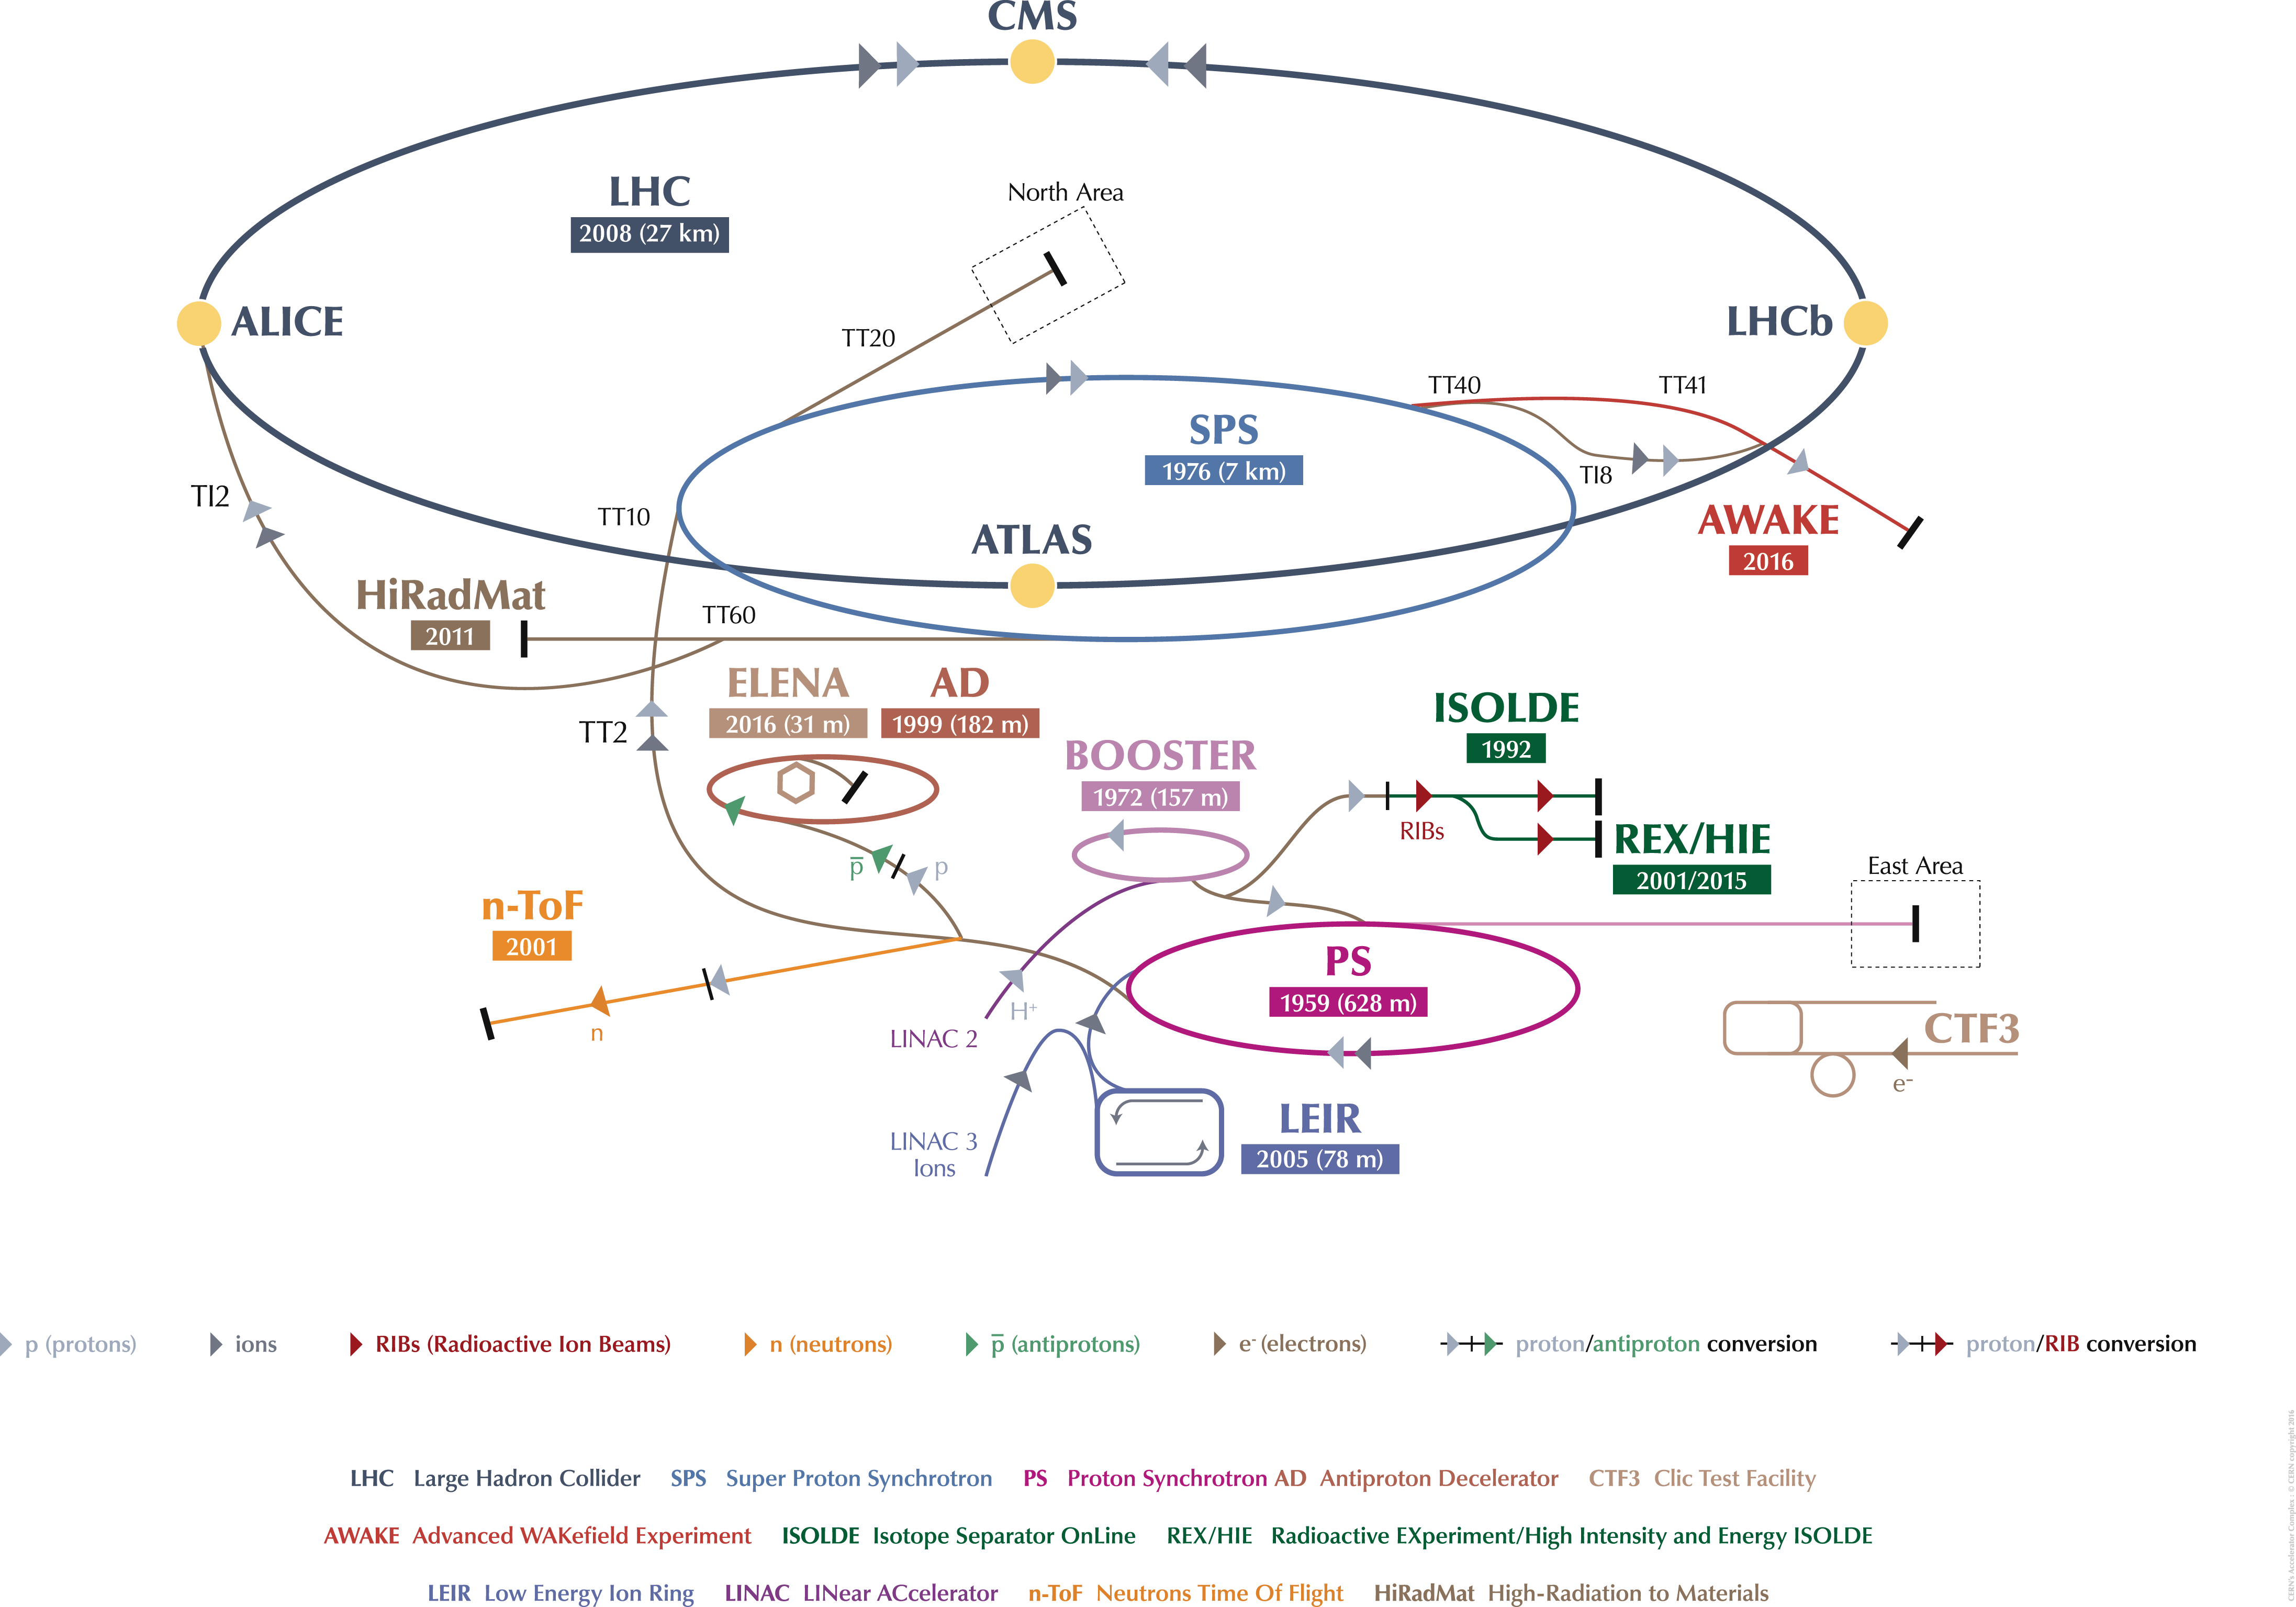
\includegraphics[trim = 0mm 70mm 0mm 0mm,clip,width=\linewidth]{figures/detector/CCC-v2016.png}
\caption{Diagram of the LHC accelerator complex.}
\label{lhcdiagram}
\end{figure}

There have been two major data taking periods of the \lhc, named \runone and \runtwo. \runone occurred between 2010 and 2012, where the centre of mass energy was $\sqrt{s}=$7~\tev (2010 and 2011) and 8~\tev (2012). Data collection for \runtwo began in 2015 and is due to end in 2018, with $\sqrt{s}=$13~\tev. At LHCb the collision conditions are designed to have roughly one proton-proton ($pp$) interaction per bunch crossing in order to allow effective primary vertex selection, necessary for the study of \B and \D meson decays, efficient track finding, and reduced radiation damage and detector occupancy. The low luminosity running is achieved by a process called {\textit{luminosity levelling}}, which involves reducing the transverse overlap of the two beams in order to reduce the area available for interactions. This allows the peak luminosity and number of $pp$ interactions per bunch crossing to be optimal, while maximising the integrated luminosity. Most of the LHCb data were recorded at an instantaneous luminosity of $4 \times 10^{32}\text{cm}^{-2}\text{s}^{-1}$, with an average of 1.7 $pp$ collisions per bunch crossing for \runone and 1.1 for \runtwo. In \runone collisions occurred at a frequency of 20 MHz, corresponding to collisions every 50~\ns, which increased to a bunch crossing rate of 40 MHz in \runtwo.

This thesis uses the complete 3~\invfb \runone dataset corresponding to 1~\invfb of $\sqrt{s} = $7~\tev data recorded in 2011 and 2~\invfb of $\sqrt{s} = $8~\tev data recorded in 2012, as well as 1.8~\invfb of the \runtwo dataset, corresponding to all of the data recorded in 2015 and 2016 at $\sqrt{s}=$13~\tev.

The \lhcb detector is designed to study particles containing \bquark and \cquark quarks. These quarks are produced dominantly via gluon interactions. The gluons typically have highly asymmetric momenta, therefore the \bquark\bquarkbar quark pair is produced predominantly in the forward (or backward) direction, illustrated in \fig\ref{bbar}. For this reason, the \lhcb detector~\cite{Alves:2008zz,LHCb-DP-2014-002} was designed as a single-arm forward spectrometer, as shown in \fig\ref{lhcbdetector}. It covers the \mbox{pseudorapidity} range $2<\eta <5$, where the pseudorapidity, $\eta$, is defined as
\begin{equation}
\eta \equiv -\ln \left[ \tan \left( \frac{\theta}{2} \right) \right] \text{ ,}
\end{equation}
where $\theta$ is the angle between the particle's momentum vector and the beam axis. This angular region captures 25\% of all \bquark\bquarkbar pairs produced. The detector is described using a right-handed coordinate system, where $z$ represents the direction of the beam into the spectrometer, $x$ points outwards from the centre of the ring and $y$ points upwards. The \lhcb spectrometer has an angular acceptance up to 300~mrad in the horizontal plane, and 250~mrad in the vertical plane. It is composed of many sub-detectors that are each specialised for a specific role. These are the Vertex Locator (\velo), the Ring Imaging Cherenkov detectors (RICH1 and RICH2), the Tracker Turicensis (TT), the dipole magnet, the tracking stations T1-T3, the calorimeter system (SPD/PS, ECAL, HCAL) and the muon stations M1-M5. In Secs.~\ref{sec:detector:velo} to \ref{sec:detector:muon}, individual descriptions of these sub-detectors are presented.

\begin{figure}
\centering
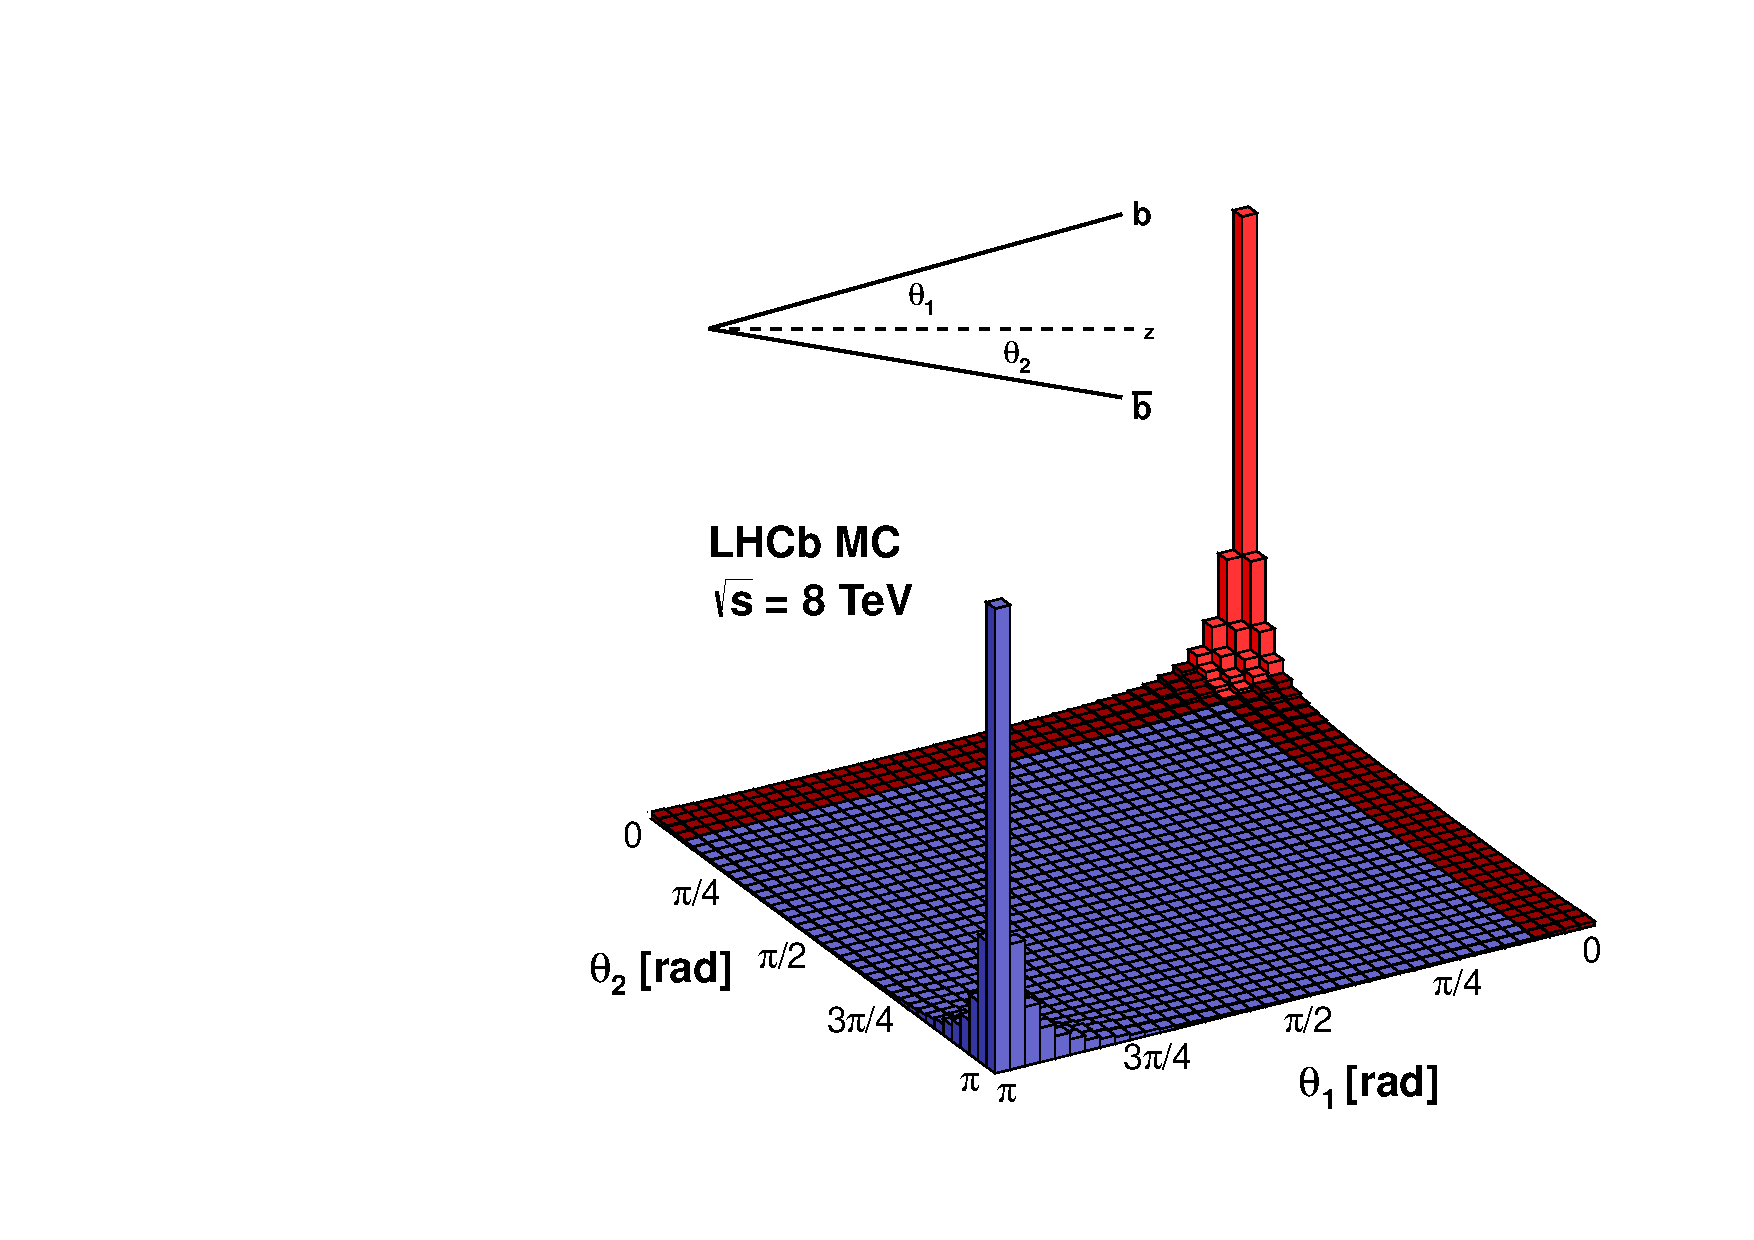
\includegraphics[width=0.5\linewidth]{figures/detector/08_rad_acc_scheme_right.pdf}
\caption{The distribution of \bquark\bquarkbar quark pair productions in simulated $pp$ collisions at 8~TeV as a function of the polar angles $\theta_1$ and $\theta_2$ with respect to the beam axis, $z$. The red shading indicates the region covered by the \lhcb detector.}
\label{bbar}
\end{figure}

\begin{figure}
\includegraphics[width=\linewidth]{figures/detector/lhcb.pdf}
\caption{Diagram of the \lhcb detector. The various sub-detectors are the Vertex Locator (\velo), the Ring Imaging Cherenkov detectors (RICH1 and RICH2), the Tracker Turicensis (TT), the dipole magnet, the tracking stations T1-T3, the calorimeter system (SPD/PS, ECAL, HCAL) and the muon stations M1-M5.}
\label{lhcbdetector}
\end{figure}

\section{The Vertex Locator}
\label{sec:detector:velo}

The Vertex Locator (\velo)~\cite{LHCb-DP-2014-001} provides precise tracking close to the \lhcb interaction region to identify primary and secondary vertices from heavy-flavour decays, which is essential for studies of long-lived particles such as \B and \D mesons. The \velo is a silicon microstrip detector situated around the $pp$ interaction point, referred to as the primary vertex (PV). It consists of 42 silicon modules arranged along the beam, each providing a measurement of the radial coordinate, $r$, and azimuthal coordinate, $\phi$, using so-called $R$ sensors and $\Phi$ sensors respectively, shown in \fig\ref{velolayout}. The sensors are located 7~\mm from the LHC beams at their closest points. The \velo modules are retracted 29~\mm in the horizontal direction during injection of the LHC beams in order to reduce radiation damage and returned to their nominal position during stable beams. The sensors are enclosed in a secondary vacuum envelope which is separated from the LHC vacuum by corrugated foil sheets designed to protect the \velo modules against electromagnetic interference from the LHC beams.

\begin{figure}
\centering
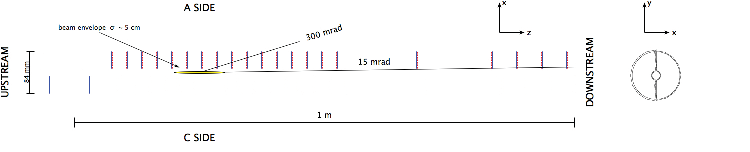
\includegraphics[width=\linewidth]{figures/detector/VELO_detector_layout_crop.pdf}
\hfill
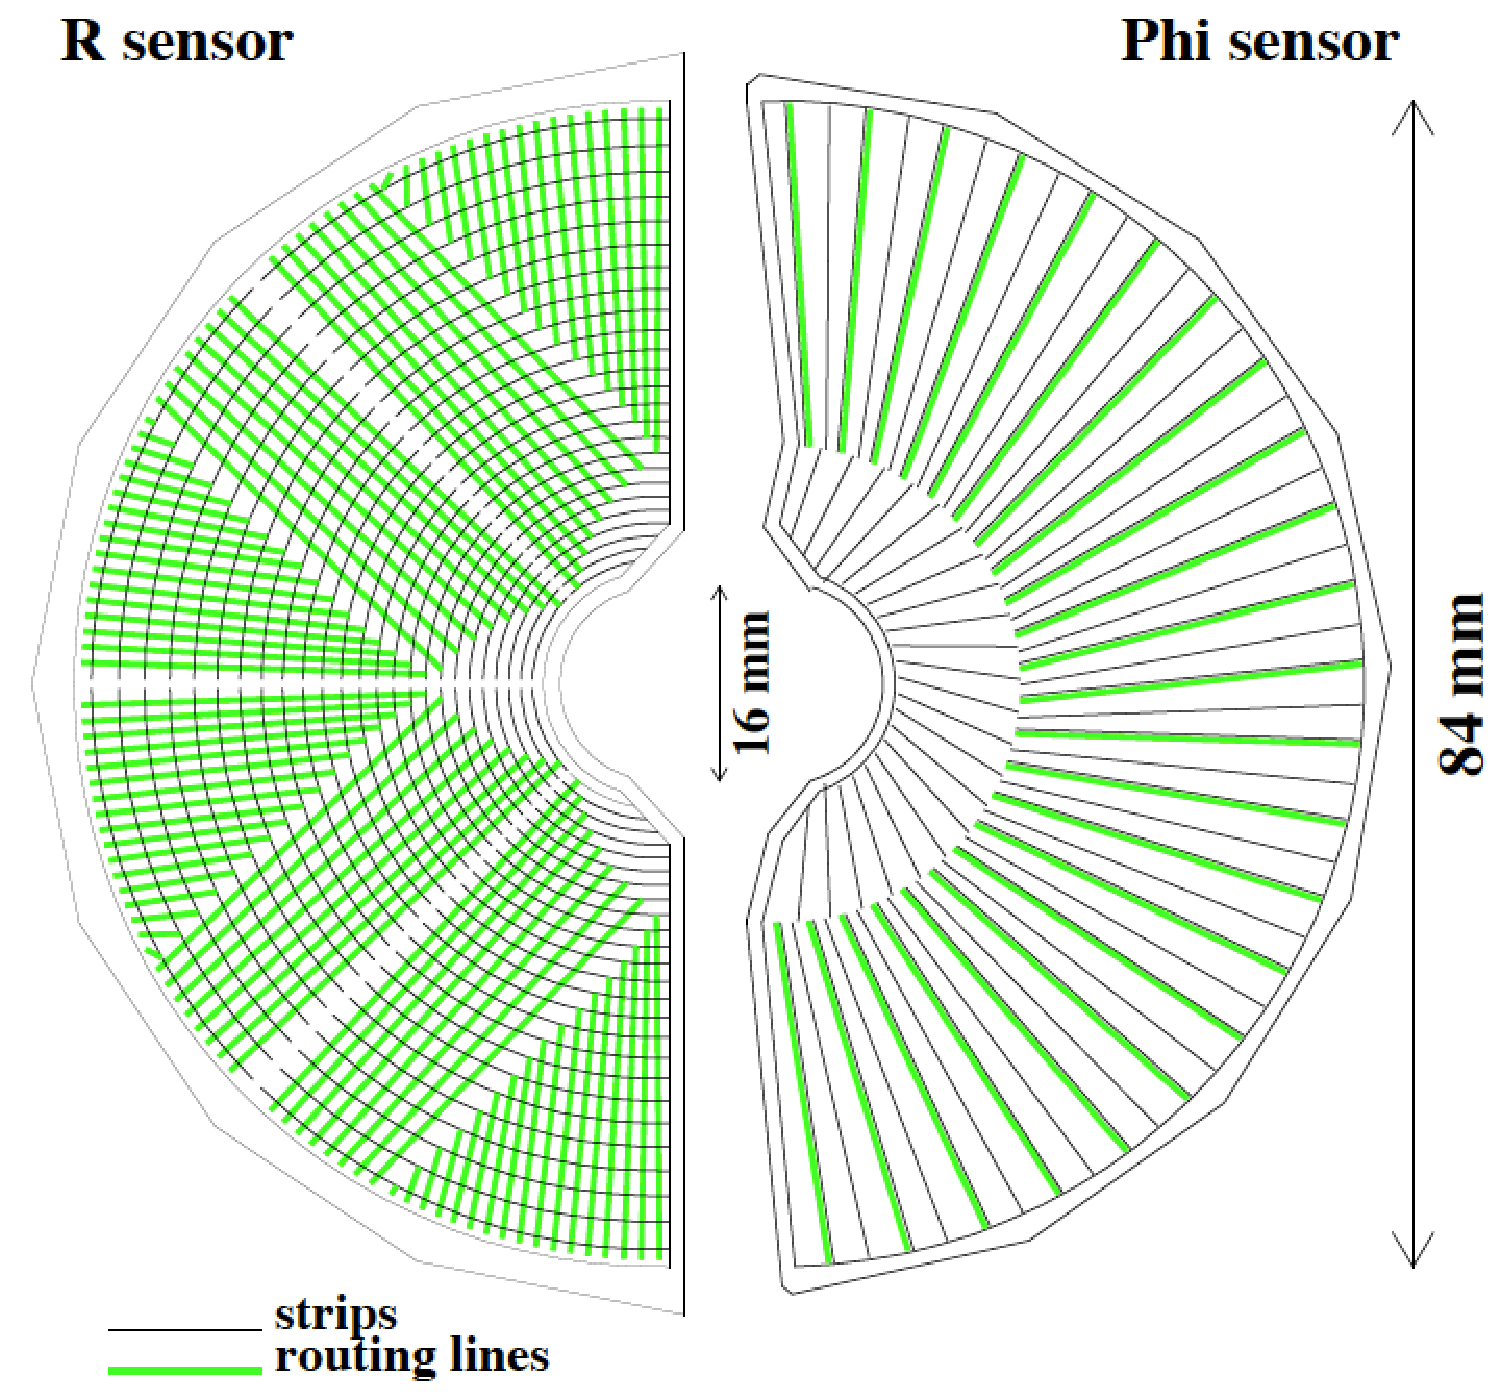
\includegraphics[width=0.3\linewidth]{figures/detector/randphisensors.pdf}
\caption{Layout of the \velo detector (top). Schematic diagram showing the $R$ and $\Phi$ sensors (bottom). Reproduced from Ref.~\cite{LHCb-DP-2014-002}.}
\label{velolayout}
\end{figure}

The \velo has a high spatial resolution, enabling precise determination of a particle's flight direction close to the primary interaction point. The impact parameter (IP) of a track is defined as the distance between the track and the PV at the track's point of closest approach to the PV. Long-lived \B and \D mesons studied in this thesis have their decay vertices displaced from the PV and as such tend to have a large IP. Therefore, the performance of the \velo can be quantified by the IP resolution, which, determined from 2012 data, is less than 35\mum for particles with transverse momentum greater than 1~\gevc~\cite{LHCb-DP-2014-001}. The IP resolution in the $x$ and $y$ directions as a function of track momentum is shown in \fig\ref{veloperformance}. The vertex resolution of the \velo is 13~\mum in the transverse plane and 71~\mum along the beam axis for vertices with 25 tracks~\cite{LHCb-DP-2014-001}.

\begin{figure}
\centering
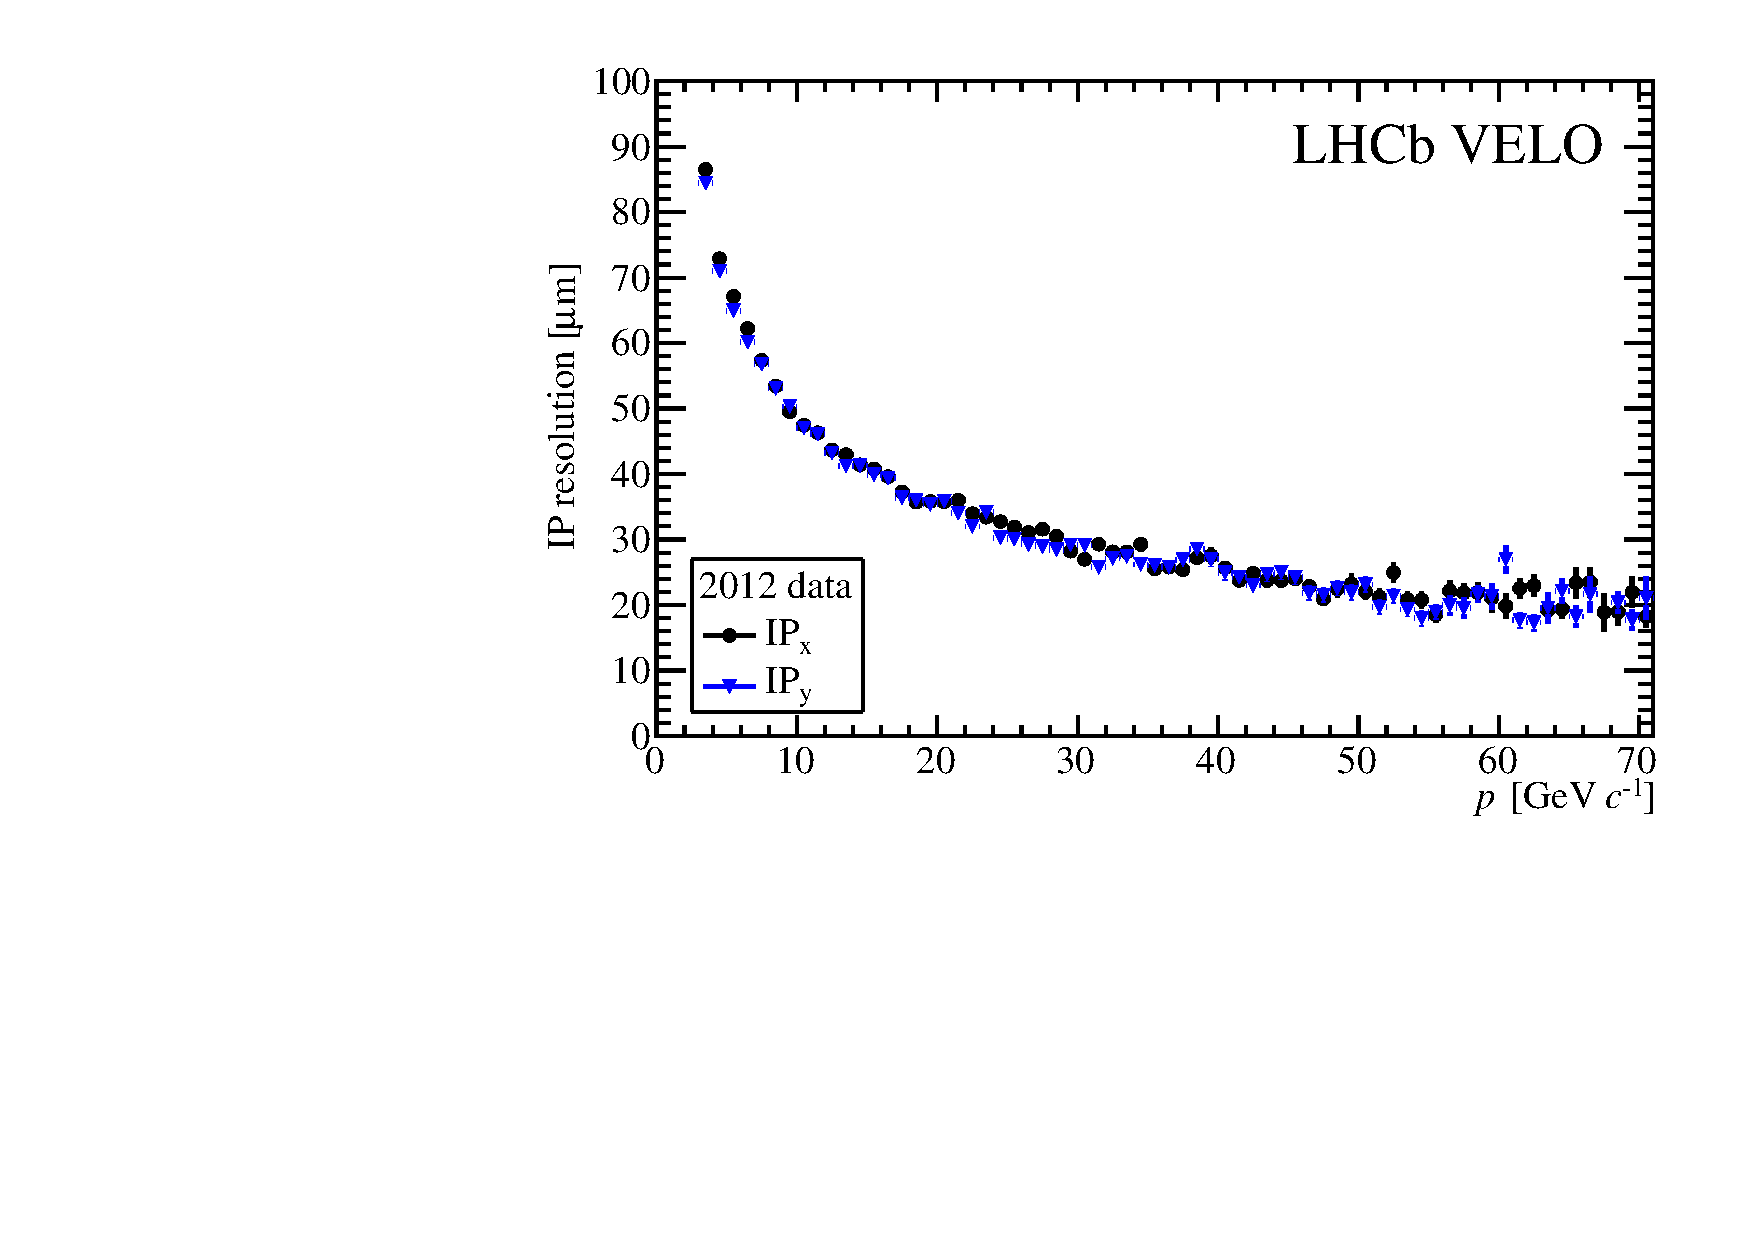
\includegraphics[width=0.5\linewidth]{figures/detector/IPRes-Vs-P-CompareIPxIPy-2012.pdf}
\caption{IP resolution as a function of momentum in both the $x$ and $y$ directions. Reproduced from Ref.~\cite{LHCb-DP-2014-001}.}
\label{veloperformance}
\end{figure}

\section{Tracking and magnet}
\label{sec:detector:tracking}

The \lhcb tracking system consists of the \velo and four planar tracking stations further downstream: the Tracker Turicensis (TT), made of silicon microstrips, upstream of the dipole magnet and tracking stations T1-T3 downstream of the magnet, as shown in \fig\ref{tracking}. The tracking stations T1-T3 have an inner region (Inner Tracker, IT) consisting of the same silicon microstrips as the TT and an outer region (Outer Tracker, OT) consisting of straw tubes. Charged particles require a minimum momentum of 1.5~\gevc to reach the tracking stations T1-T3.

\begin{figure}
\centering
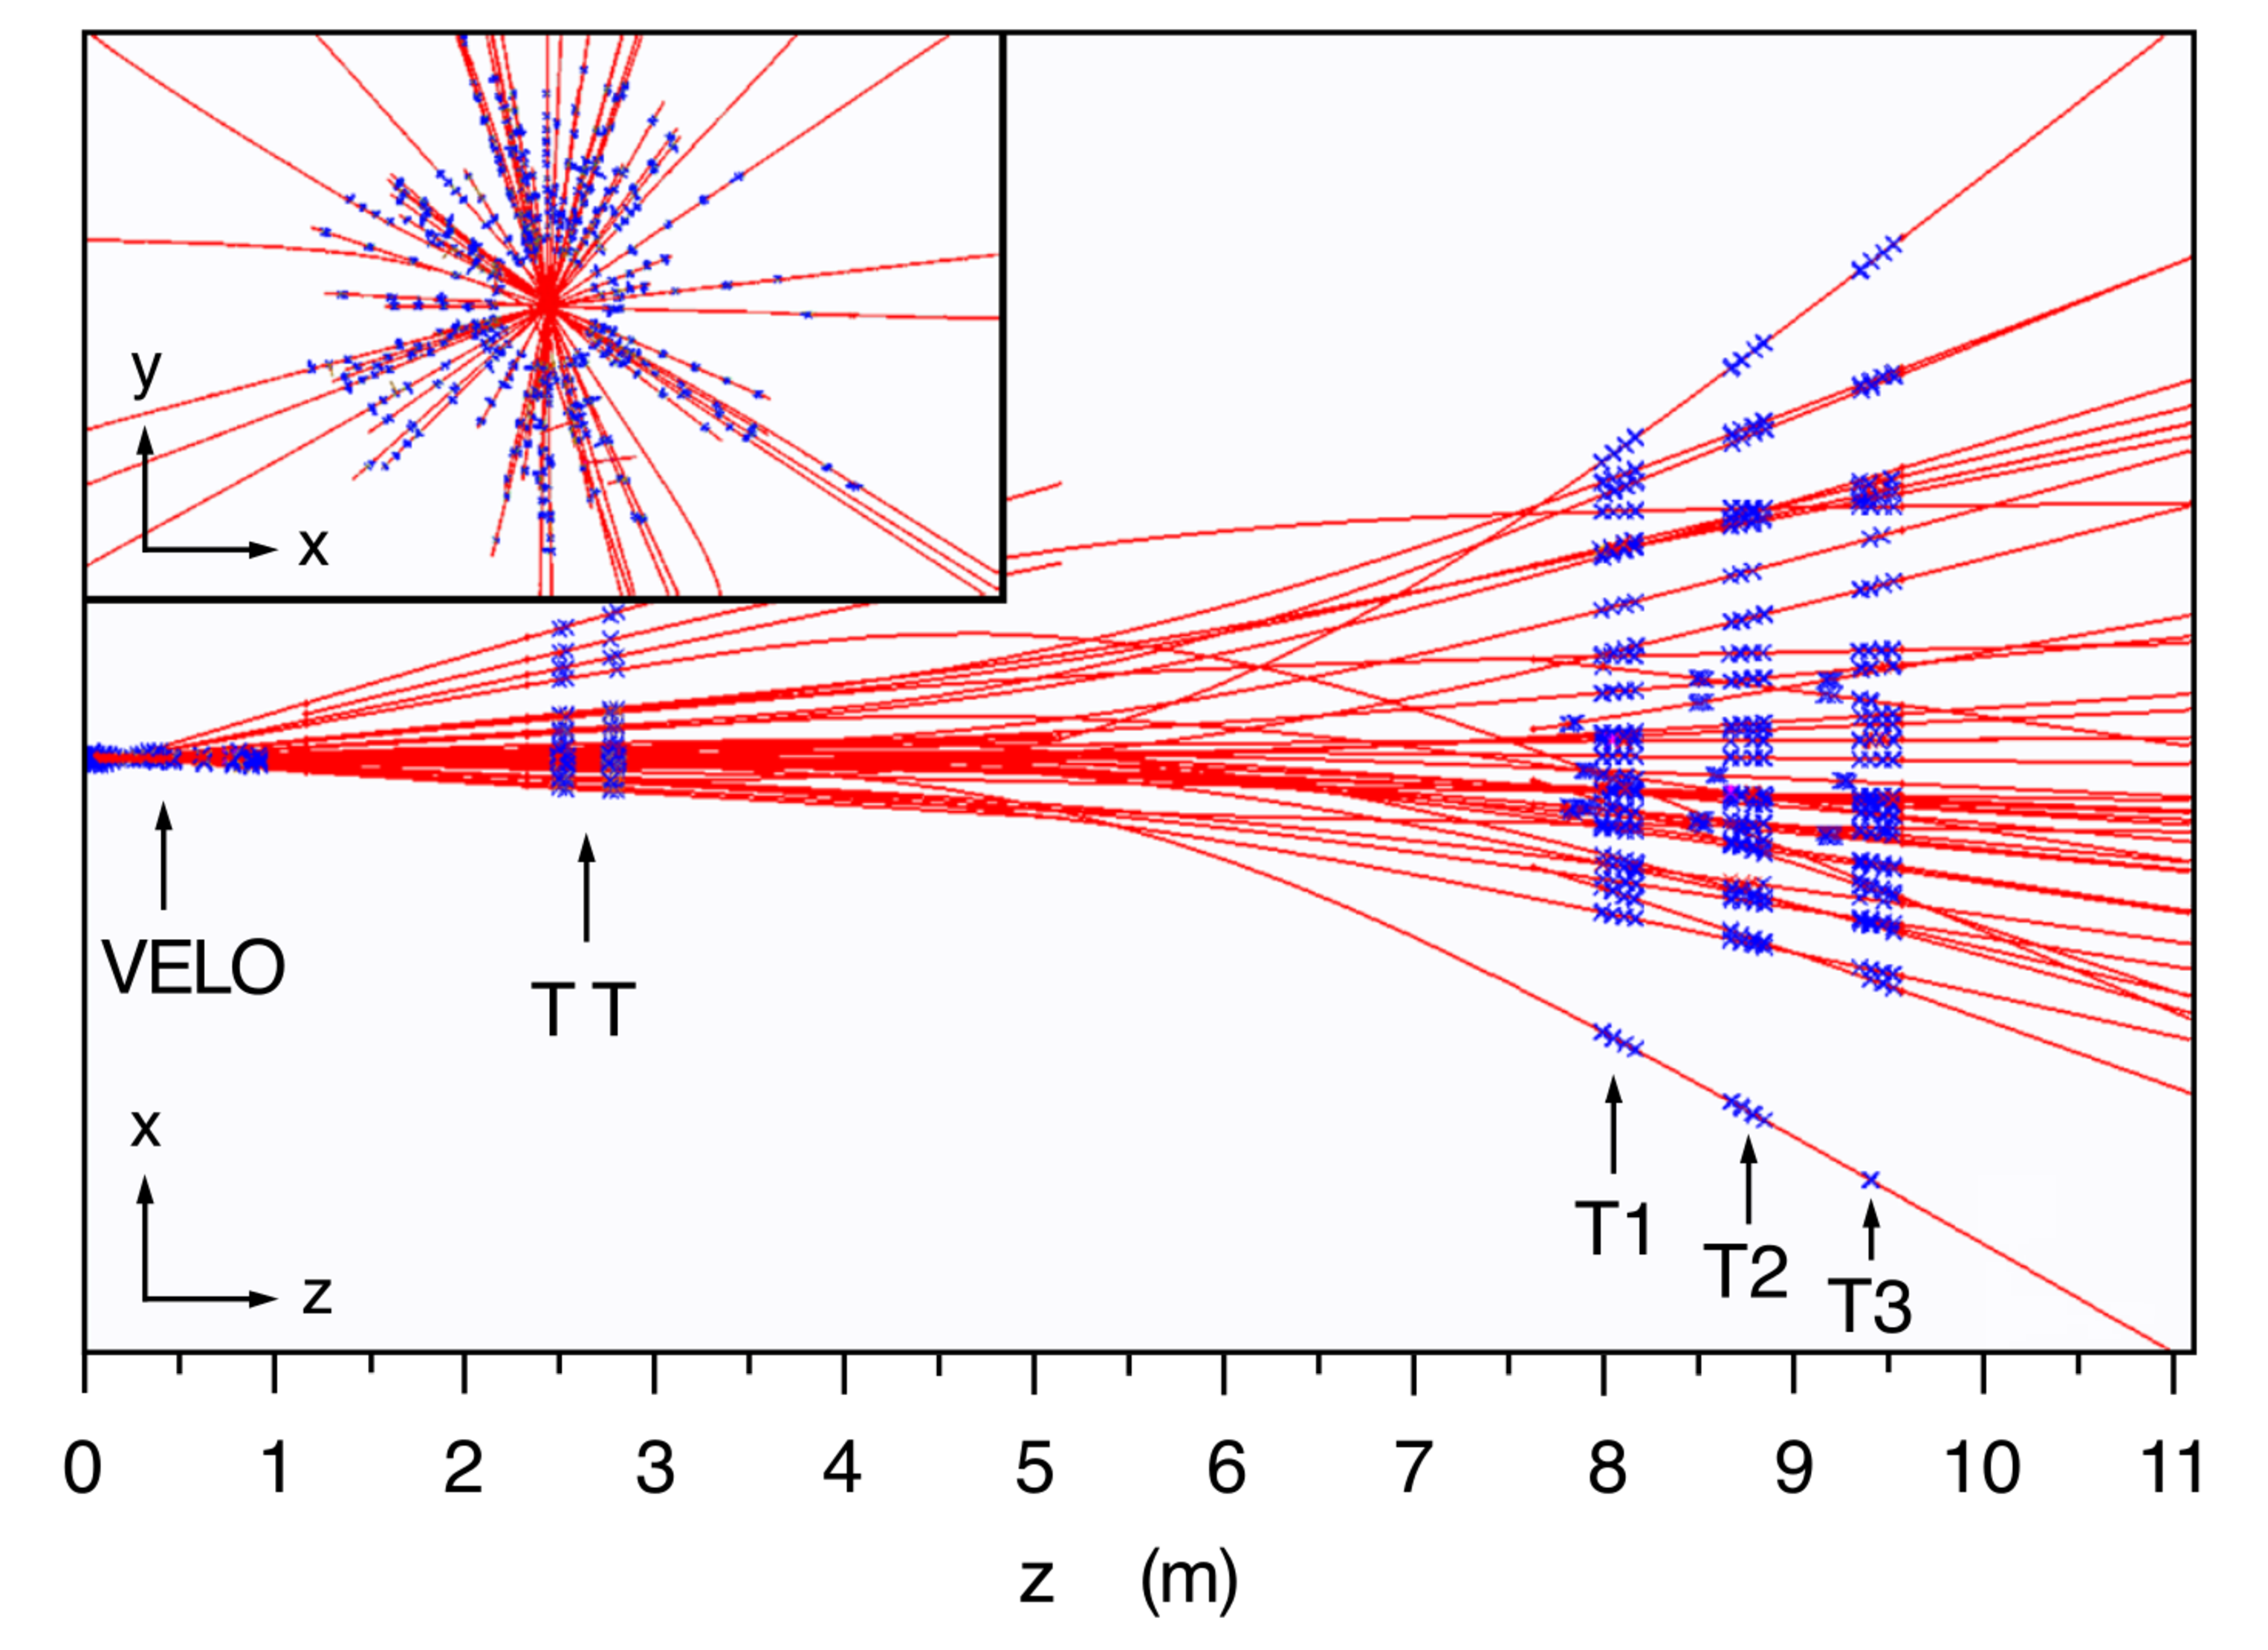
\includegraphics[width=0.7\linewidth]{figures/detector/tracking.pdf}
\caption{Display of the reconstructed tracks (red) and assigned hits (blue) in an event in the $x-z$ plane. The insert shows a zoom into the \velo region in the $x-y$ plane. Reproduced from Ref \cite{LHCb-DP-2014-002}.}
\label{tracking}
\end{figure}

The TT and IT are constructed from silicon microstrip detectors, arranged as shown in \fig\ref{itandot}. The TT is a planar detector 150\cm wide and 130\cm high, located upstream of the dipole magnet, covering the full detector acceptance. At the centre of each of the three T-stations downstream of the magnet, the IT is arranged in a cross shape, 120~\cm wide and 40~\cm high, around the beam pipe. Each of the four planar tracking stations are composed of four layers of modules with the first and fourth layers mounted vertically and the second and third layers mounted at $+5^{\circ}$ and $-5^{\circ}$ from the vertical, respectively. The TT has an active area of 8.4\ma and the IT has an active area of 4.0\ma, and both use silicon microstrip sensors with a strip pitch of about
200\mum, giving a single hit resolution of around 50\mum.

The OT is a straw drift tube detector for the tracking of charged particles and the measurement of their momentum over the full detector acceptance. The straw tubes in each station are arranged in four modules, with the same rotation of modules as in the TT and IT. Each module contains two staggered layers of drift-tubes. The total active area is approximately 6$\times$5~\mma and contains approximately 55,000 single straw-tube channels, with inner diameters of 4.9~\mm. The straw tubes are filled with a gas mixture containing 70\% argon and 30\% carbon dioxide, which guarantees a drift time below 50~\ns and sufficient drift-coordinate resolution of 200~\mum.

\begin{figure}
\centering
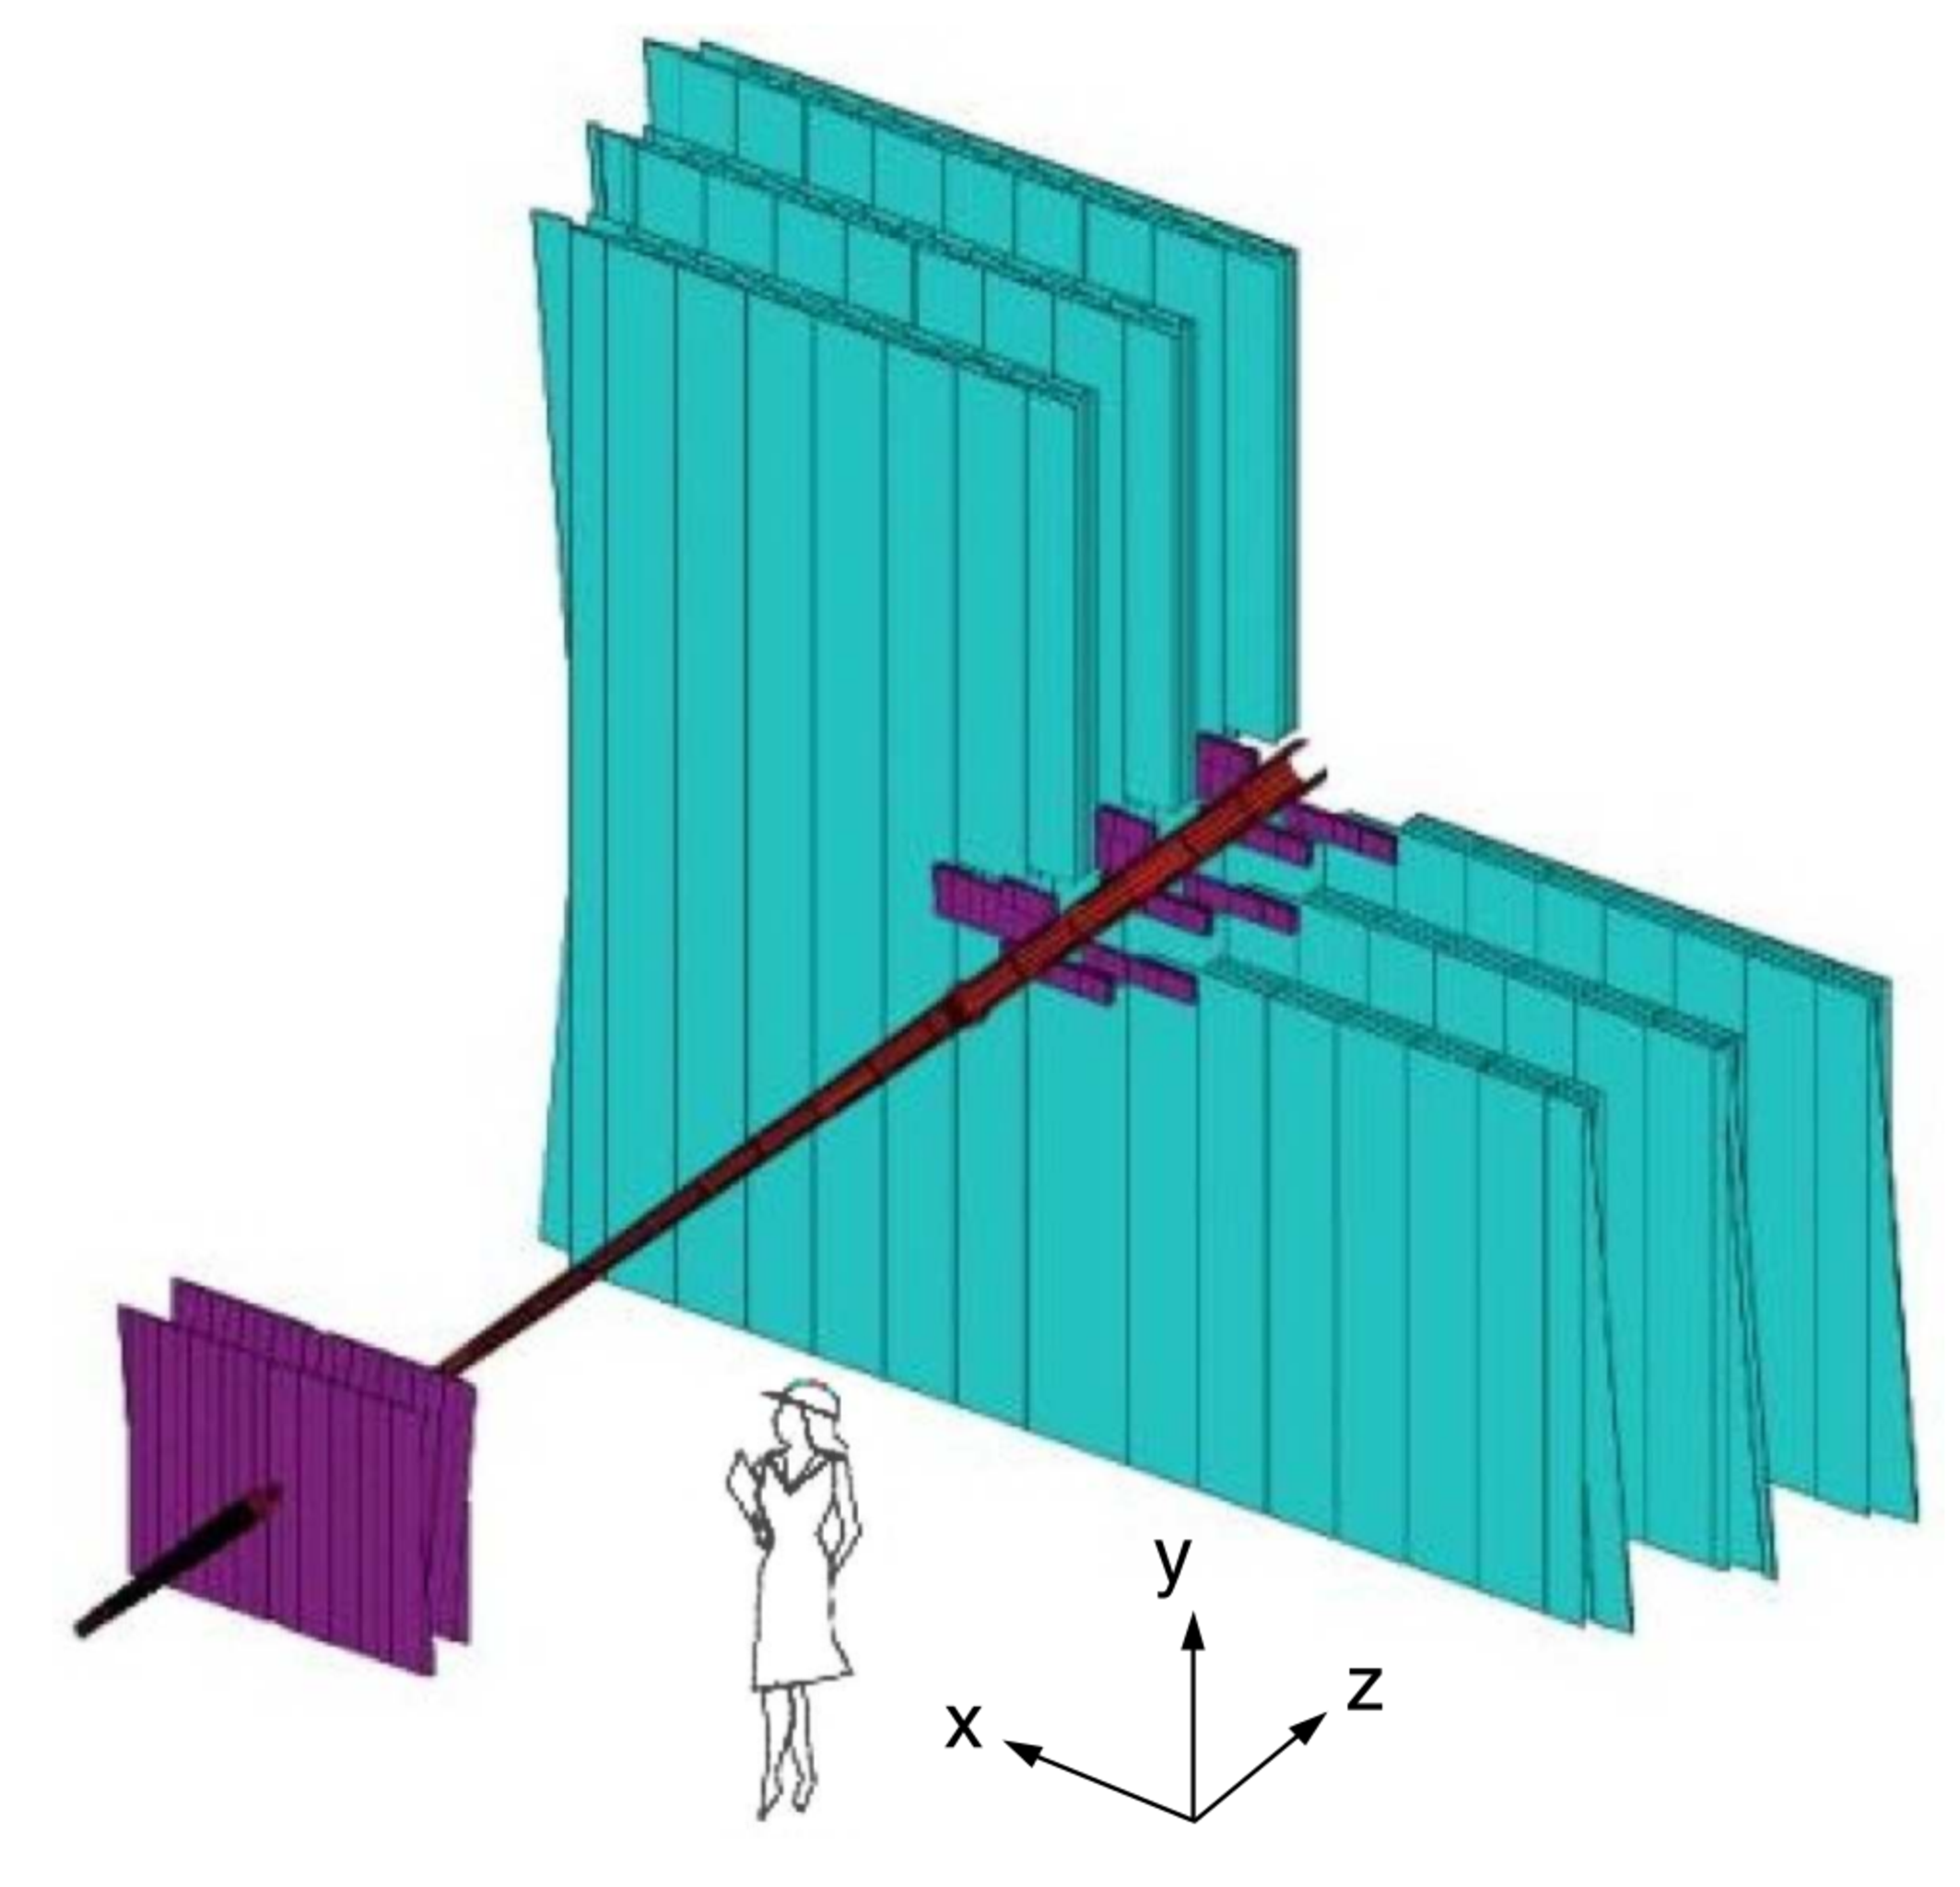
\includegraphics[width=0.5\linewidth]{figures/detector/InnerAndOuterTracker.pdf}
\caption{Arrangement of the layers of the IT and OT. Reproduced from Ref.~\cite{lhcbdetector2008}.}
\label{itandot}
\end{figure}

The dipole magnet, with an integrated magnetic field of about 4~Tm, enables the momentum of charged particles to be measured by bending the trajectory of charged particles in the horizontal plane. In order to achieve the required momentum resolution, the integrated magnetic field, $B = \int{\mathcal{B} dl}$, is measured to a precision corresponding to $\delta B /B \sim 10^{-4}$, where $\mathcal{B}$ is the magnetic field density. Since positively and negatively charged particles will bend in opposite directions, a charge detection asymmetry can result if the left and right halves of the detector have different tracking efficiencies. This would affect \CP violation studies, such as the one described in this thesis, which involve the measurements of charge asymmetries. Hence, to minimise systematics, the magnetic field direction is reversed regularly during data-taking.

The tracking efficiency is defined as the probability that the trajectory of a charged particle that passes through the full tracking system is reconstructed. The measured tracking efficiency as a function of momentum and pseudorapidity is shown in \fig\ref{trackingeff}. The average efficiency is above 96\% over the momentum range 5 - 200~\gevc and pseudorapidity range, 2 $< \eta <$ 5. \Fig\ref{momentumres} shows the momentum resolution of reconstructed tracks, which is about 0.5\% for particles below 20~\gevc, rising to about 0.8\% for particles around 100 \gevc. 
%In \runone, the efficiency of the OT to detect a hit in the central half of the straw is estimated to be 99.2\%, and the position resolution is determined to be approximately 200~\mum~\cite{LHCb-DP-2013-003}. 

\begin{figure}
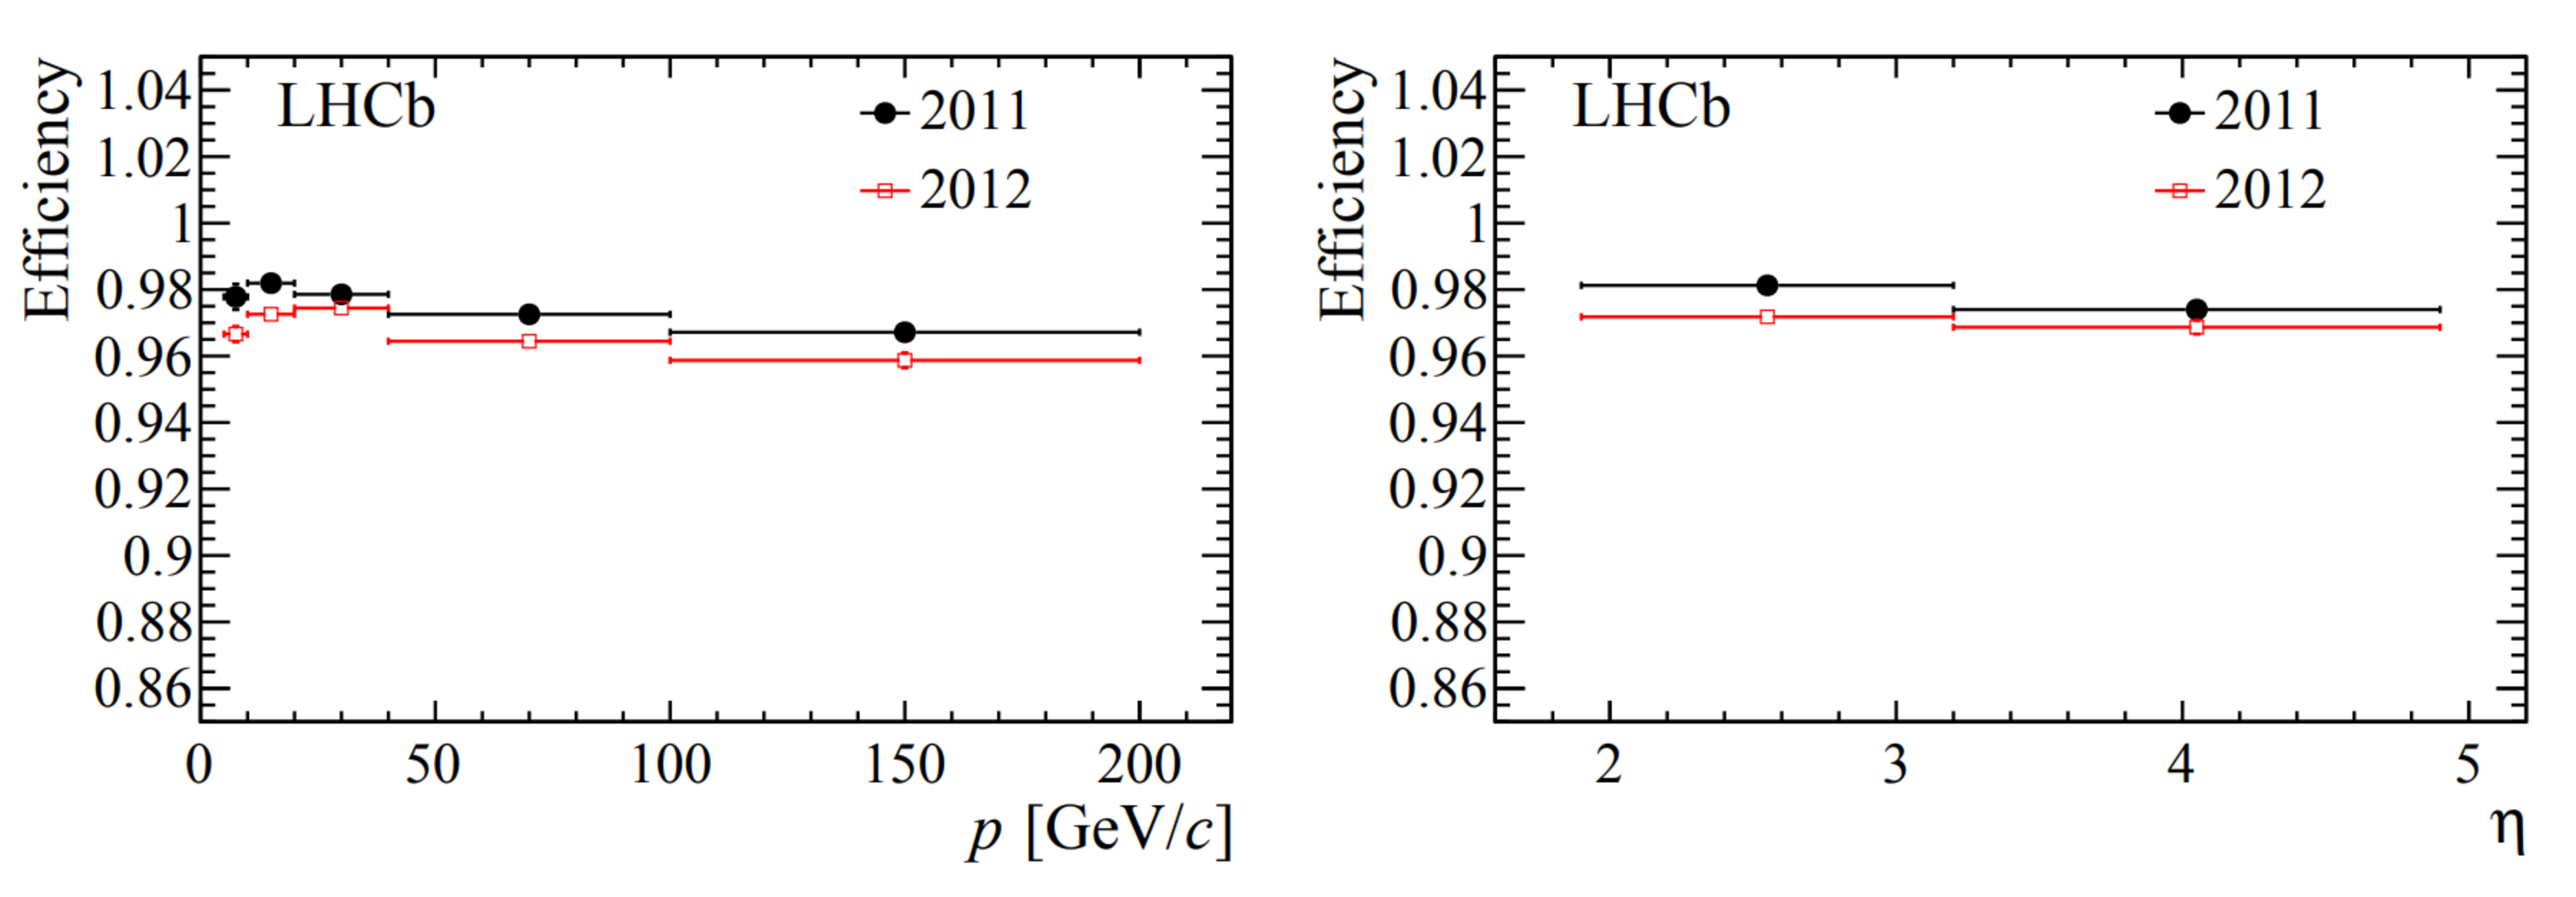
\includegraphics[width=\linewidth]{figures/detector/trackingefficiency.pdf}
\caption{Tracking efficiency as a function of momentum, $p$, and pseudorapidity, $\eta$. The error bars indicate the statistical uncertainty. Reproduced from Ref.~\cite{LHCb-DP-2013-002}.}
\label{trackingeff}
\end{figure}

\begin{figure}
\centering
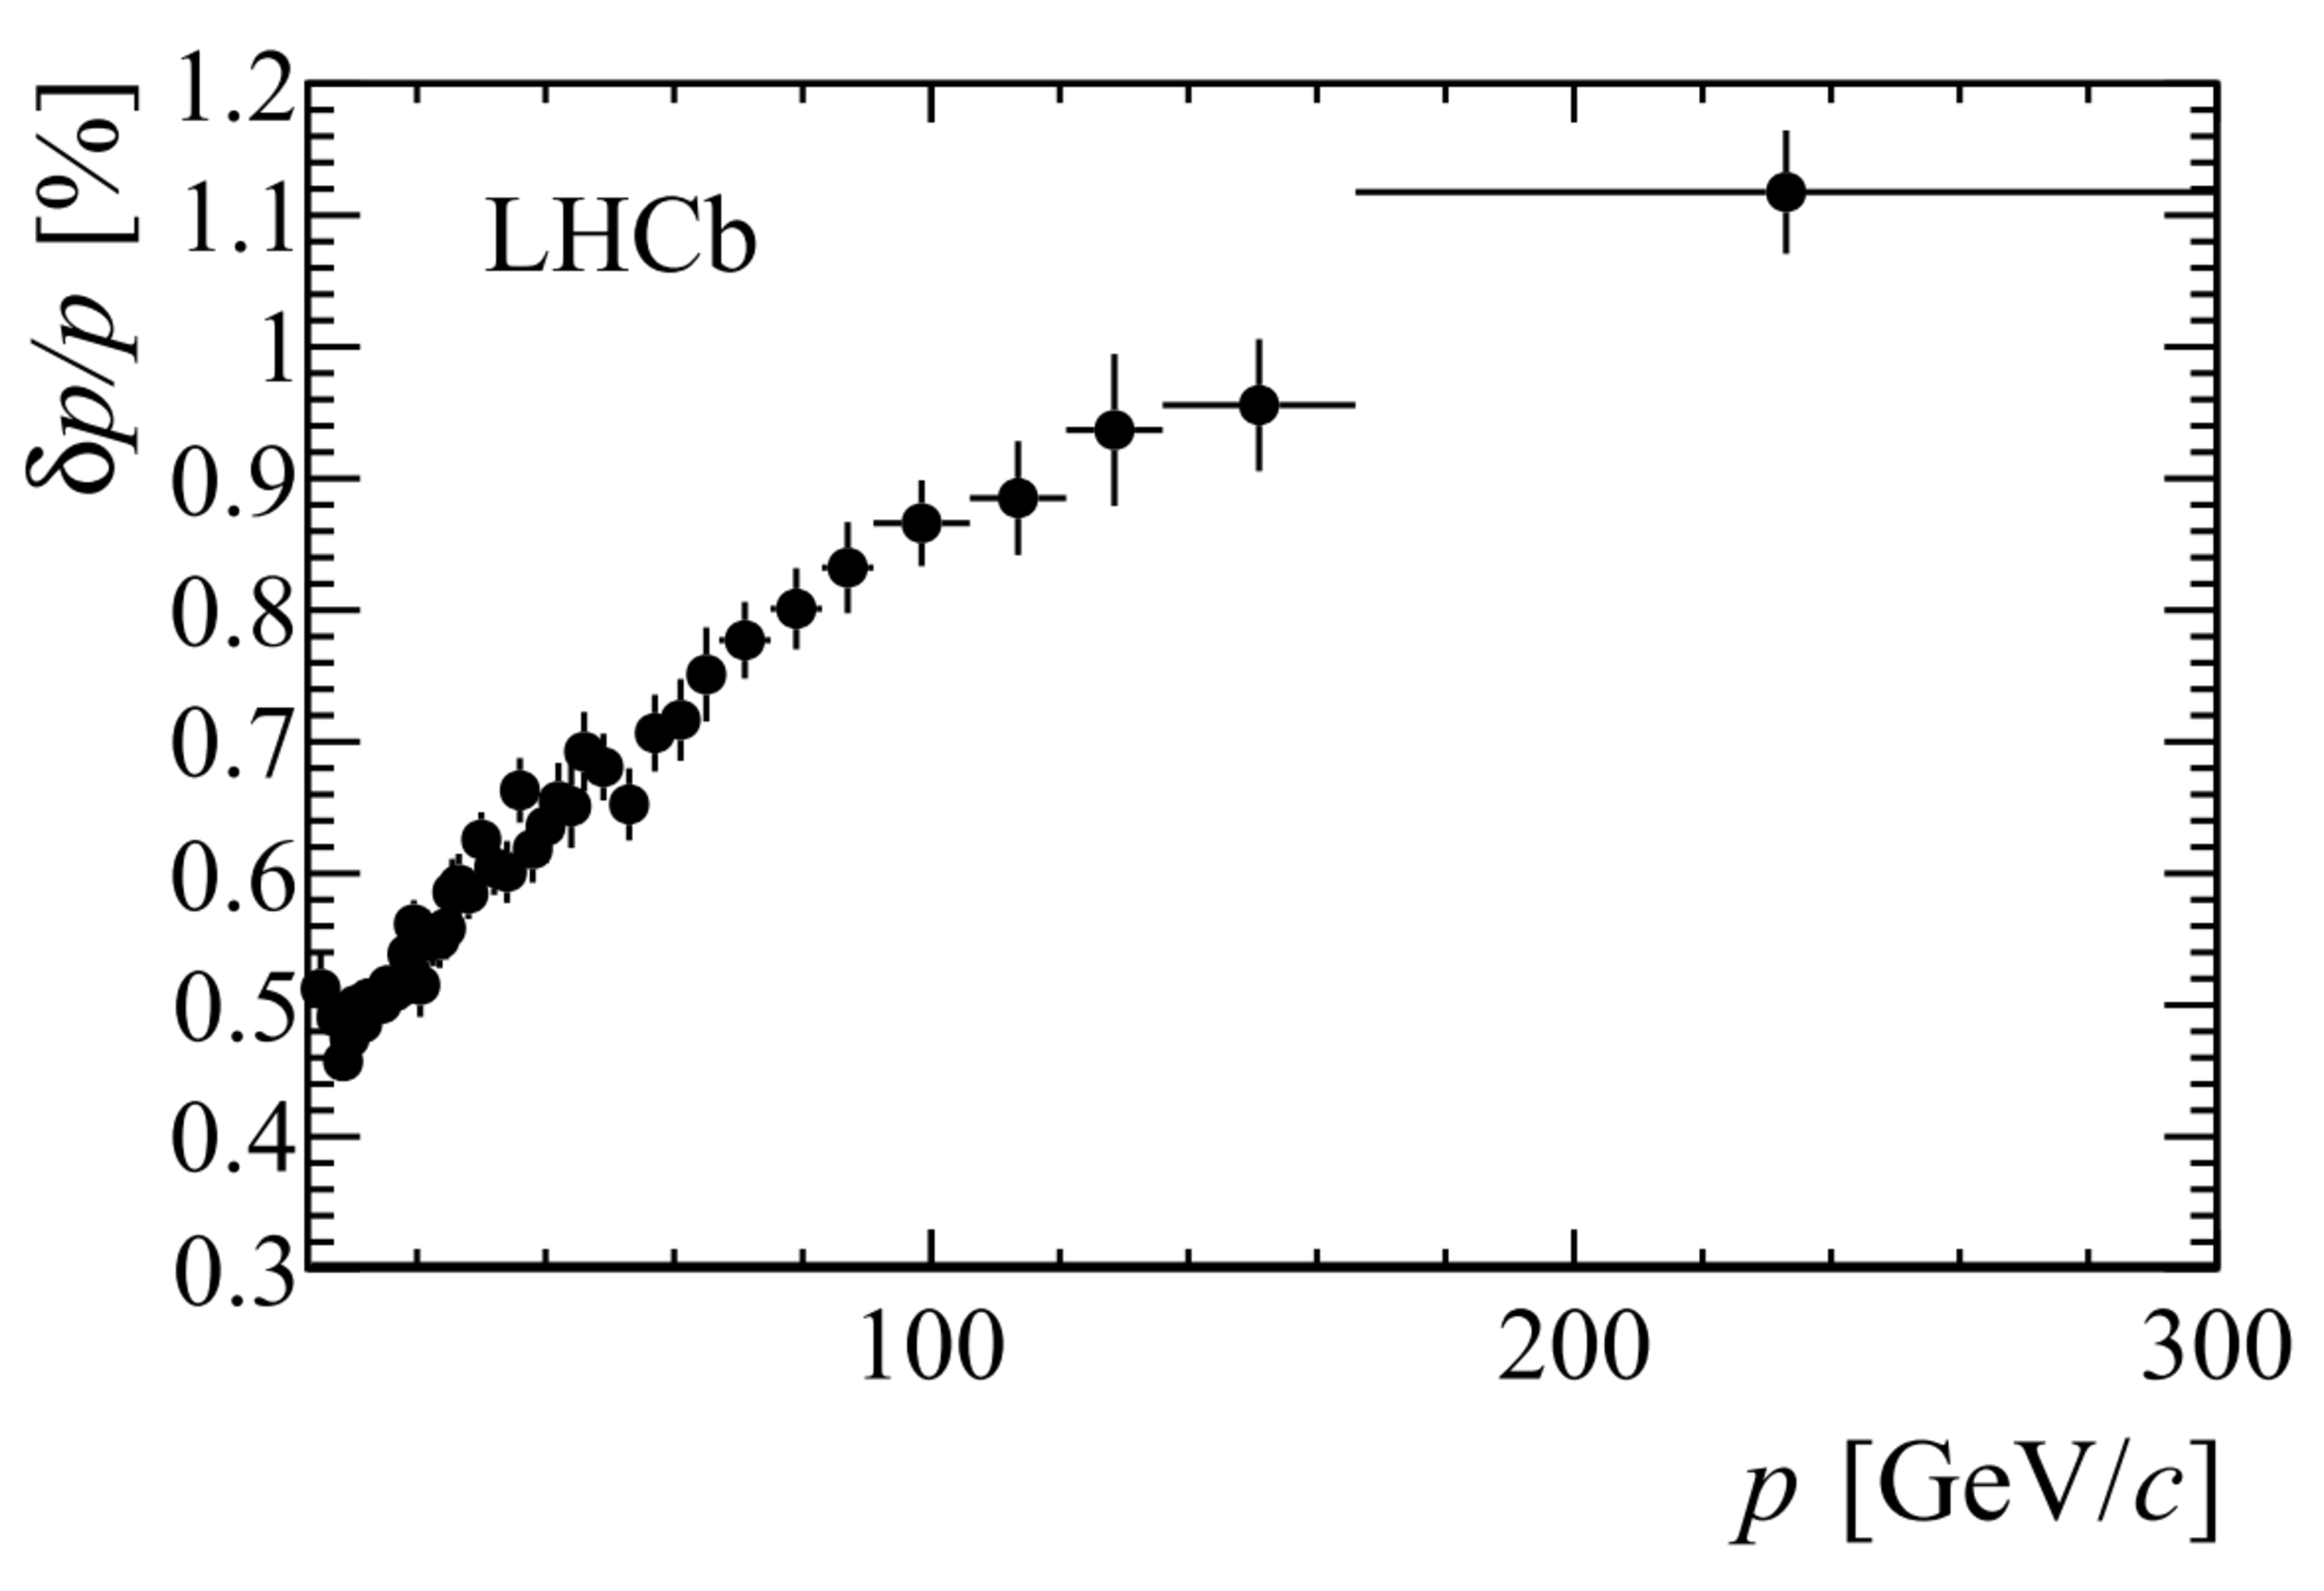
\includegraphics[width=0.5\linewidth]{figures/detector/momentumresolution.pdf}
\caption{Momentum resolution as a function of momentum for tracks that have traversed the entire tracking system. Reproduced from Ref \cite{LHCb-DP-2014-002}.}
\label{momentumres}
\end{figure}
	
\section{The \rich detectors}
\label{sec:detector:rich}

The \rich detectors (RICH 1 and RICH 2)~\cite{LHCb-DP-2012-003} are required for the identification of charged hadrons, specifically pions, kaons and protons. The decay modes of \bquark- and \cquark-flavoured hadrons involve hadronic multibody final states, therefore good particle identification of hadrons over the momentum range 2 - 100 \gevc is vital for reducing the combinatorial backgrounds. The RICH detectors utilise the idea that Cherenkov radiation is produced whenever a charged particle of velocity $v$, travelling through a dielectric medium of refractive index $n$, exceeds the speed of light in that medium, $c/n$. The particle produces a cone of light with an opening angle of $\theta_{CK}$ relative to the direction of the particle's propagation, given by
\begin{equation}
\cos\left(\theta_{CK}\right) = \frac{1}{n\beta} \text{ ,     where }  \beta = v/c \text{ .}
\label{cherenkov}
\end{equation}
By measuring $\theta_{CK}$ using the \rich detectors and the momentum from the magnet and tracking systems, a mass hypothesis can be determined, which provides discrimination between particle species. The relationship between Cherenkov angle and momentum for different particle species is shown in \fig\ref{richseparation}. It can be seen that the separation tends to zero as the momentum increases, as expected from \eqn\ref{cherenkov}, since as $\beta \rightarrow 1$, the Cherenkov angle becomes independent of particle momentum and mass. For a given dielectric medium, there is a low momentum threshold, defined when $\beta = 1/n$, where below this value of $\beta$ no Cherenkov light is emitted. Discrimination of lower momentum (higher mass) particles is then only possible with a dielectric medium of higher refractive index.

\begin{figure}
\centering
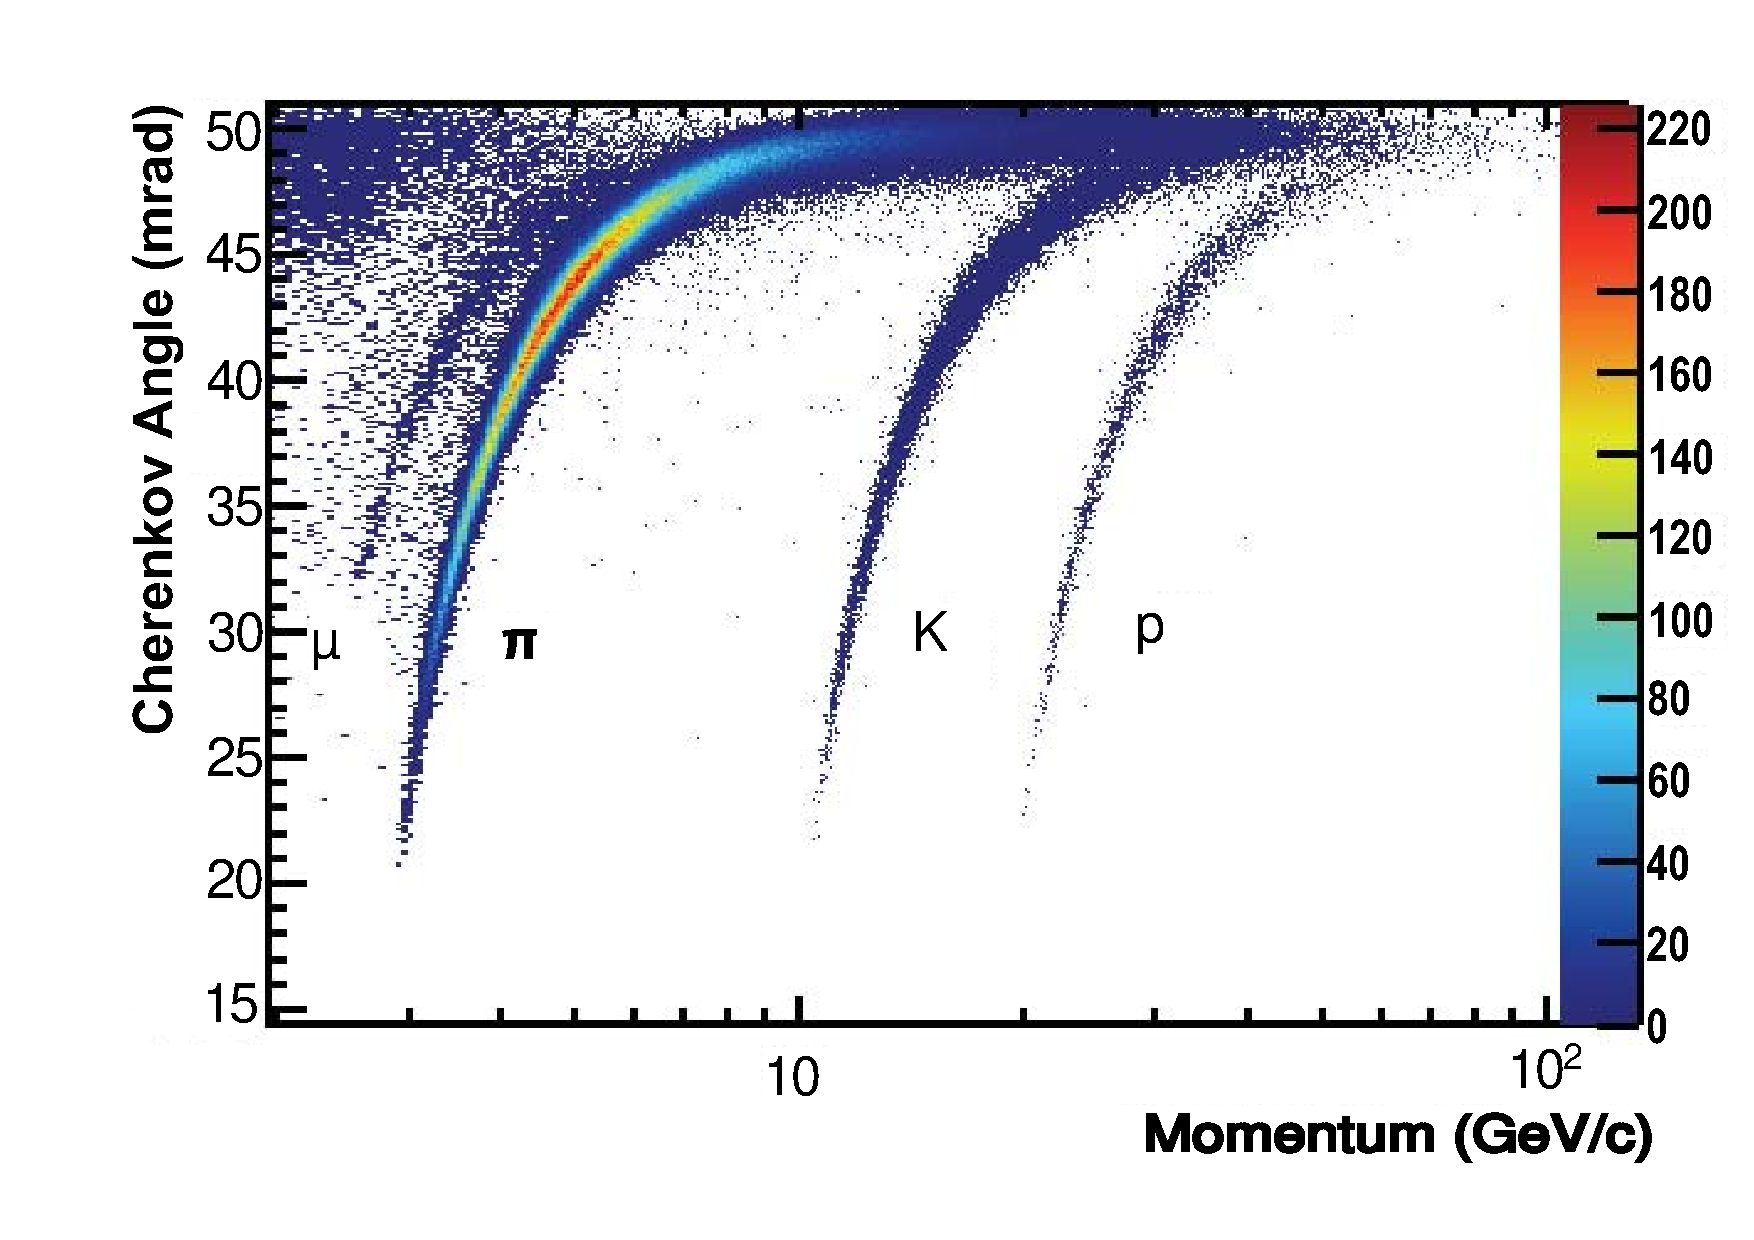
\includegraphics[width=0.8\linewidth]{figures/detector/richseparation.pdf}
\caption{Cherenkov angle measured as a function of momentum in the RICH1 $C_{4}F_{10}$ radiator for isolated tracks. The Cherenkov bands for muons, pions, kaons and protons are clearly visible. Reproduced from Ref \cite{LHCb-DP-2012-003}.}
\label{richseparation}
\end{figure}

Two \rich detectors are used to cover the full \lhcb momentum range; RICH 1 is positioned upstream of the magnet covering the momentum range 2 to 60~\gevc, using two radiators: C$_4$F$_{10}$ ($n = 1.0014$) and Aerogel ($n = 1.03$) in Run 1, although the Aerogel radiator was subsequently removed for Run 2. RICH 2 is located downstream of the magnet and covers the higher momentum range, 15 to 100~\gevc, utilising a CF$_4$ radiator ($n = 1.0005$). While RICH 1 covers the full detector acceptance, RICH 2 covers a limited angular acceptance of $~\sim \pm 15$~mrad to $\pm 120$~mrad in the horizontal direction and $\pm 100$~mrad in the vertical direction. In each RICH detector the cone of Cherenkov radiation that radiates from the charged particle is reflected by spherical focusing primary mirrors and planar secondary mirrors to project a ring onto the focal plane containing an array of Hybrid Photon Detectors (HPDs). The HPDs contain pixels of area $2\times 2$~\mma, which detect the single photons.

One of the main measures of the \rich performance is the resolution of the Cherenkov angle from which the hit positions of the photons can be reconstructed. This is measured from the distribution of the difference between the measured and expected Cherenkov angle for each photon, $\Delta\theta$, given by $\theta_{CK} - \theta_0$, where $\theta_0$ is the expected Cherenkov angle calculated from the momentum of the track and the refractive index of the radiator. \Fig\ref{cherenkov} shows an example of the distributions of $\Delta\theta$, and from these plots the Cherenkov angle resolution is determined to be $(1.618 \pm 0.002)$~mrad for C$_4$F$_{10}$ in RICH1 and $(0.68 \pm 0.02)$~mrad for CF$_4$ in RICH2.

\begin{figure}
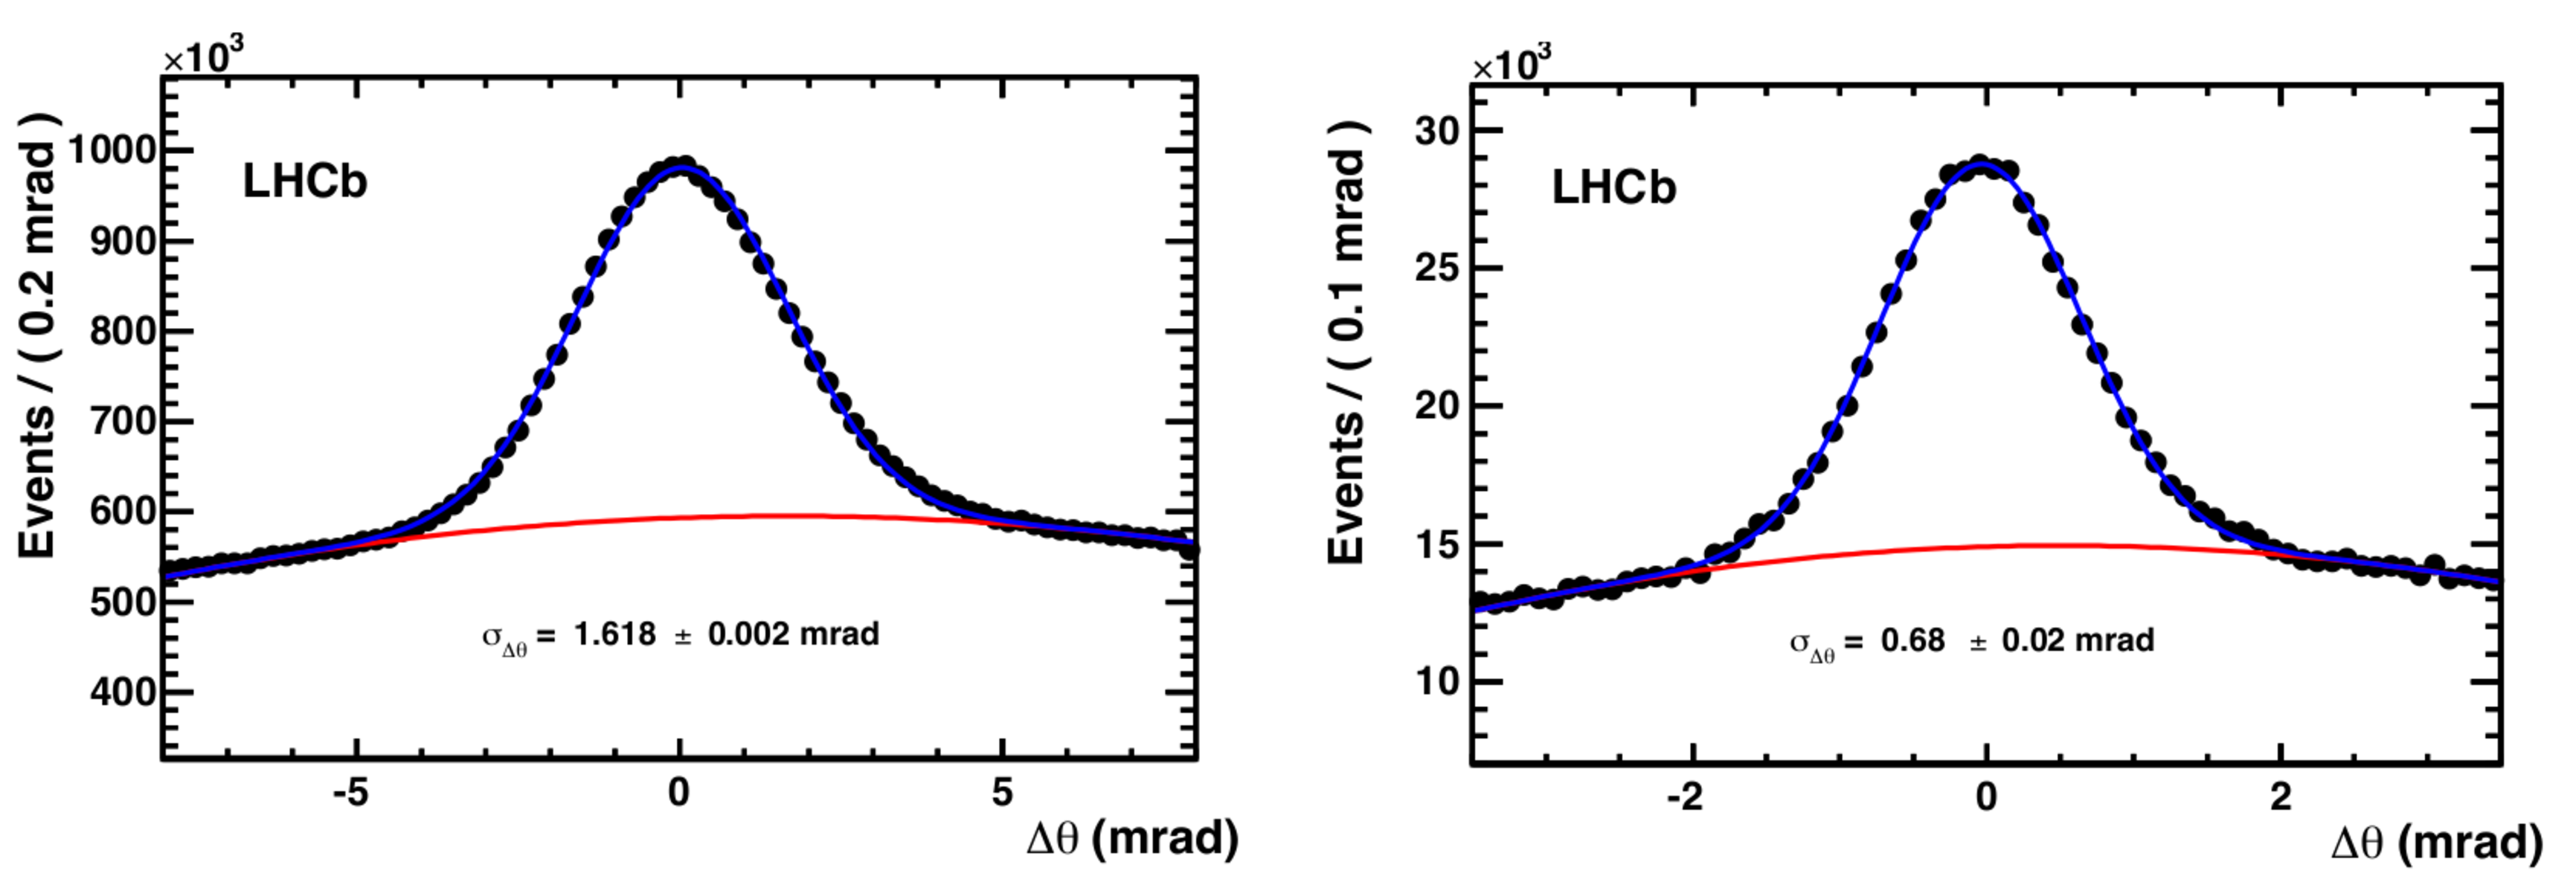
\includegraphics[width=\linewidth]{figures/detector/cherenkov.pdf}
\caption{Cherenkov angle resolution using 2011 data for the RICH 1 gas (left) and RICH 2 gas (right). Reproduced from Ref \cite{LHCb-DP-2012-003}.}
\label{cherenkov}
\end{figure}

Although the RICH system is designed primarily to provide separation between charged hadrons (\pion, $K$ and $p$), it can also provide some information on leptons. Similarly, the calorimeters and muon systems, described below, can provide some hadron identification. A global likelihood hypothesis for each particle type (\pion, $K$, $p$, $e$, $\mu$) is formed by combining the particle likelihood hypotheses as determined by each sub-detector, $\mathcal{L}_X$, for particle hypothesis $X$. Since the most abundant particles from a $pp$ interaction are pions, the pion hypothesis is initially assumed. For each track the differences between a particle hypothesis, $X$, log-likelihood compared to the pion hypothesis is computed:
\begin{equation}
DLLX = \log{\mathcal{L}_X} - \log{\mathcal{L}_{\pi}} \text{ .}
\end{equation}

The PID performance of hadrons can be directly determined from background-free calibration samples of protons, kaons and pions, for example, those produced in \Lz, \Dstarm and \KS decays respectively. The typical kaon PID performance of the \lhcb detector for both \runone and \runtwo is shown in \fig\ref{richperformance}. It can be seen that the overall performance of the \rich system has improved in \runtwo. These improvements from \runone to \runtwo are both due to changes in the running conditions, for example the increase in beam energy and the change in trigger conditions, and the intrinsic performance of the \rich system, mainly from the removal of the aerogel radiator.

\begin{figure}
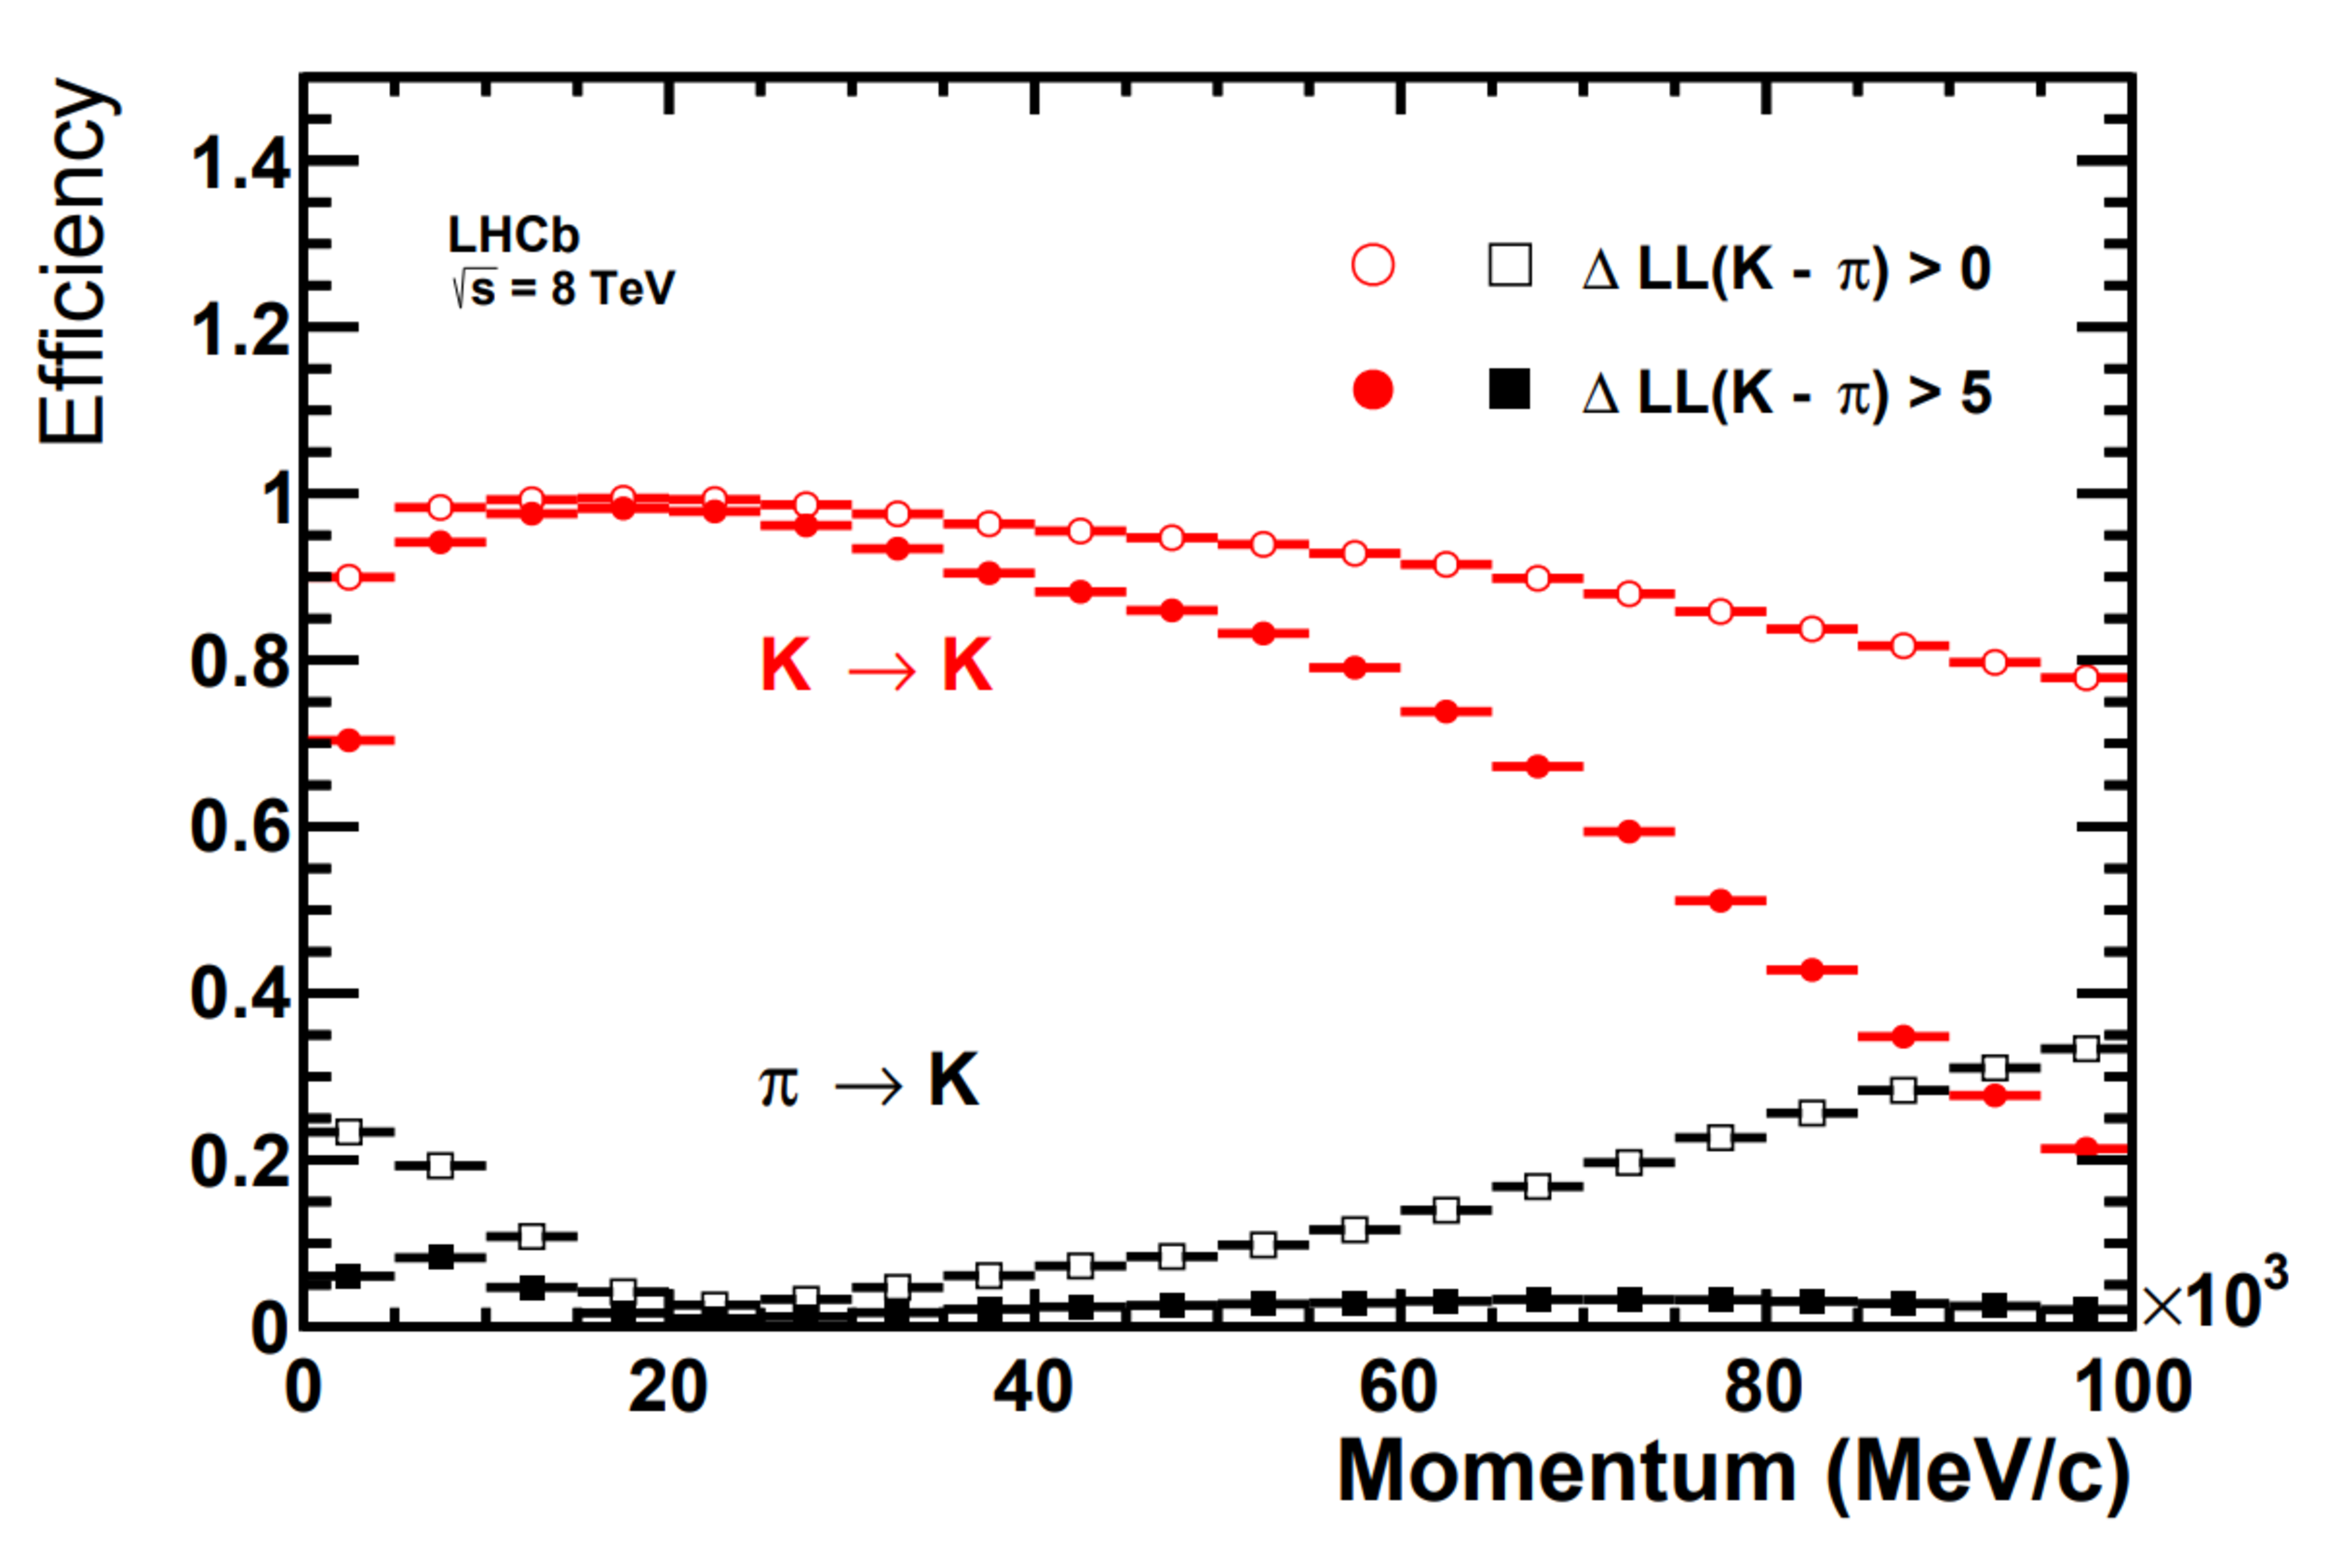
\includegraphics[width=0.5\linewidth]{figures/detector/richperformance_run1.pdf}
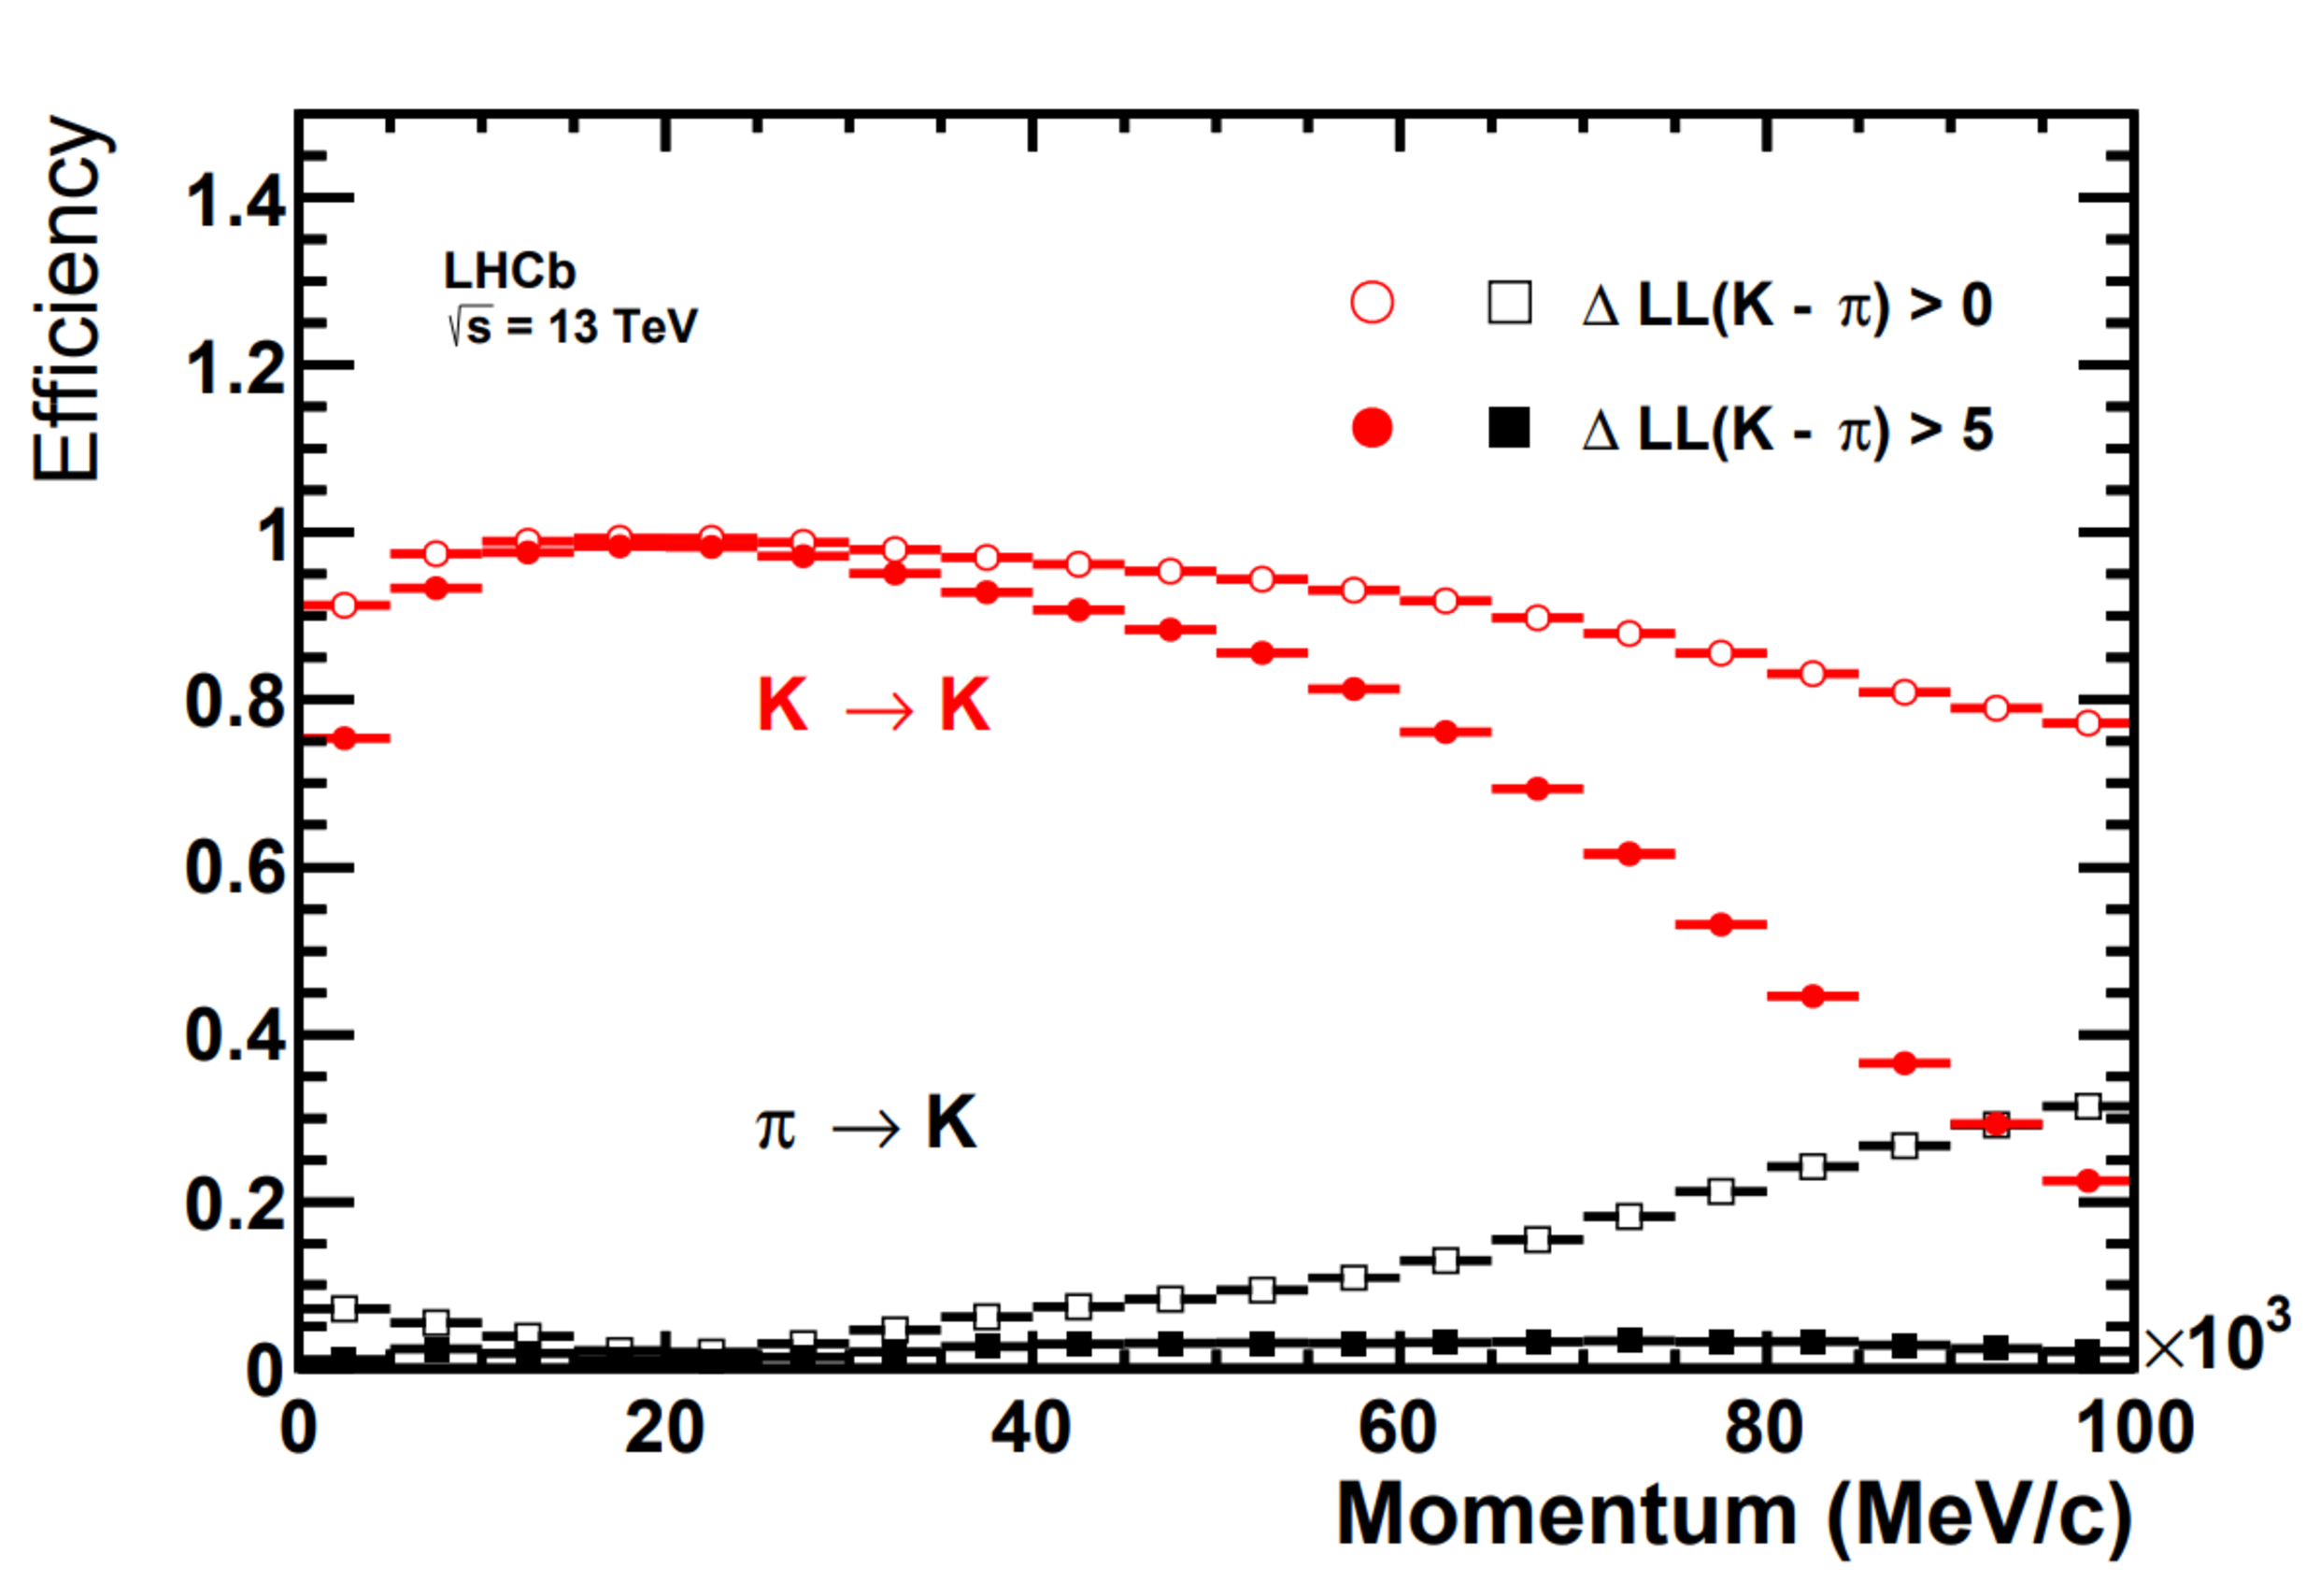
\includegraphics[width=0.5\linewidth]{figures/detector/richperformance_run2.pdf}
\caption{Kaon PID performance of the \rich system as a function of momentum in both \runone (left) and \runtwo (right), showing the efficiency to correctly identify kaons (red points) and the corresponding pion misidentification probability (black points). The expression $\Delta \text{LL}(K - \pi)$ is equivalent to $\log{\mathcal{L}_K} - \log{\mathcal{L}_{\pi}}$, described in the text. Reproduced from Ref \cite{richrun2}.}
\label{richperformance}
\end{figure}

\section{Calorimeters}

The \lhcb calorimeter system provides energy measurements and is essential for the first level of the trigger to select particles with high transverse energy. It consists of four sub-systems: the scintillating-pad (SPD) and pre-shower (PS) detectors, the electromagnetic calorimeter (ECAL) and the hadronic calorimeter (HCAL)~\cite{LHCb-DP-2013-004}. All subsystem components provide energy measurements using the mechanism of detecting scintillation light using photomultiplier tubes (PMTs). The calorimeter system is located downstream of RICH 2, between the first two muon stations, as shown in \fig\ref{lhcbdetector}. The ECAL is required to measure electrons and photons and the HCAL to measure charged and neutral hadrons.  The SPD/PS detectors are nearest the interaction point and designed to help the ECAL with electron identification. Between the SPD and PS is a 15~\mm lead converter, 2.5 radiation lengths thick, to initiate showering before the PS. 

The ECAL is composed of 4~\mm thick alternating lead absorber and polystyrene scintillator layers with an acceptance of 300~mrad horizontally and 250~mrad vertically. The thickness of the ECAL corresponds to 25 radiation lengths, chosen to fully contain high energy photon showers for optimum energy resolution. The energy resolution of the ECAL is parameterised by $\sigma E/E = (8.5-9.5\%)/\sqrt{E} \oplus 0.8\%$, for energy, $E$, in \gev~\cite{calo_latest}.

The HCAL has its scintillating tiles mounted parallel to the beam axis to increase the contact area between the scintillator tiles and optical fibres, maximising the amount of scintillation light collected. The tiles are separated by 100~m thick iron absorber plates. Due to space limitations, the HCAL has a thickness limited to 5.6 nuclear interaction lengths. The measured energy resolution is $\sigma_E/E = (69 \pm 5)\%/\sqrt{E} \oplus (9 \pm 2)\%$ for energy, $E$, in \gev~\cite{calo_latest}.

All four components of the calorimeter system are composed of scintillator pads with a cell granularity that decreases when moving outwards from the beam pipe, as shown in \fig\ref{calorimeter}. The SPD/PS and ECAL have variable segmentation split into three sections, whereas the HCAL is split into two zones with larger cell sizes due to the larger size of hadronic showers.

\begin{figure}
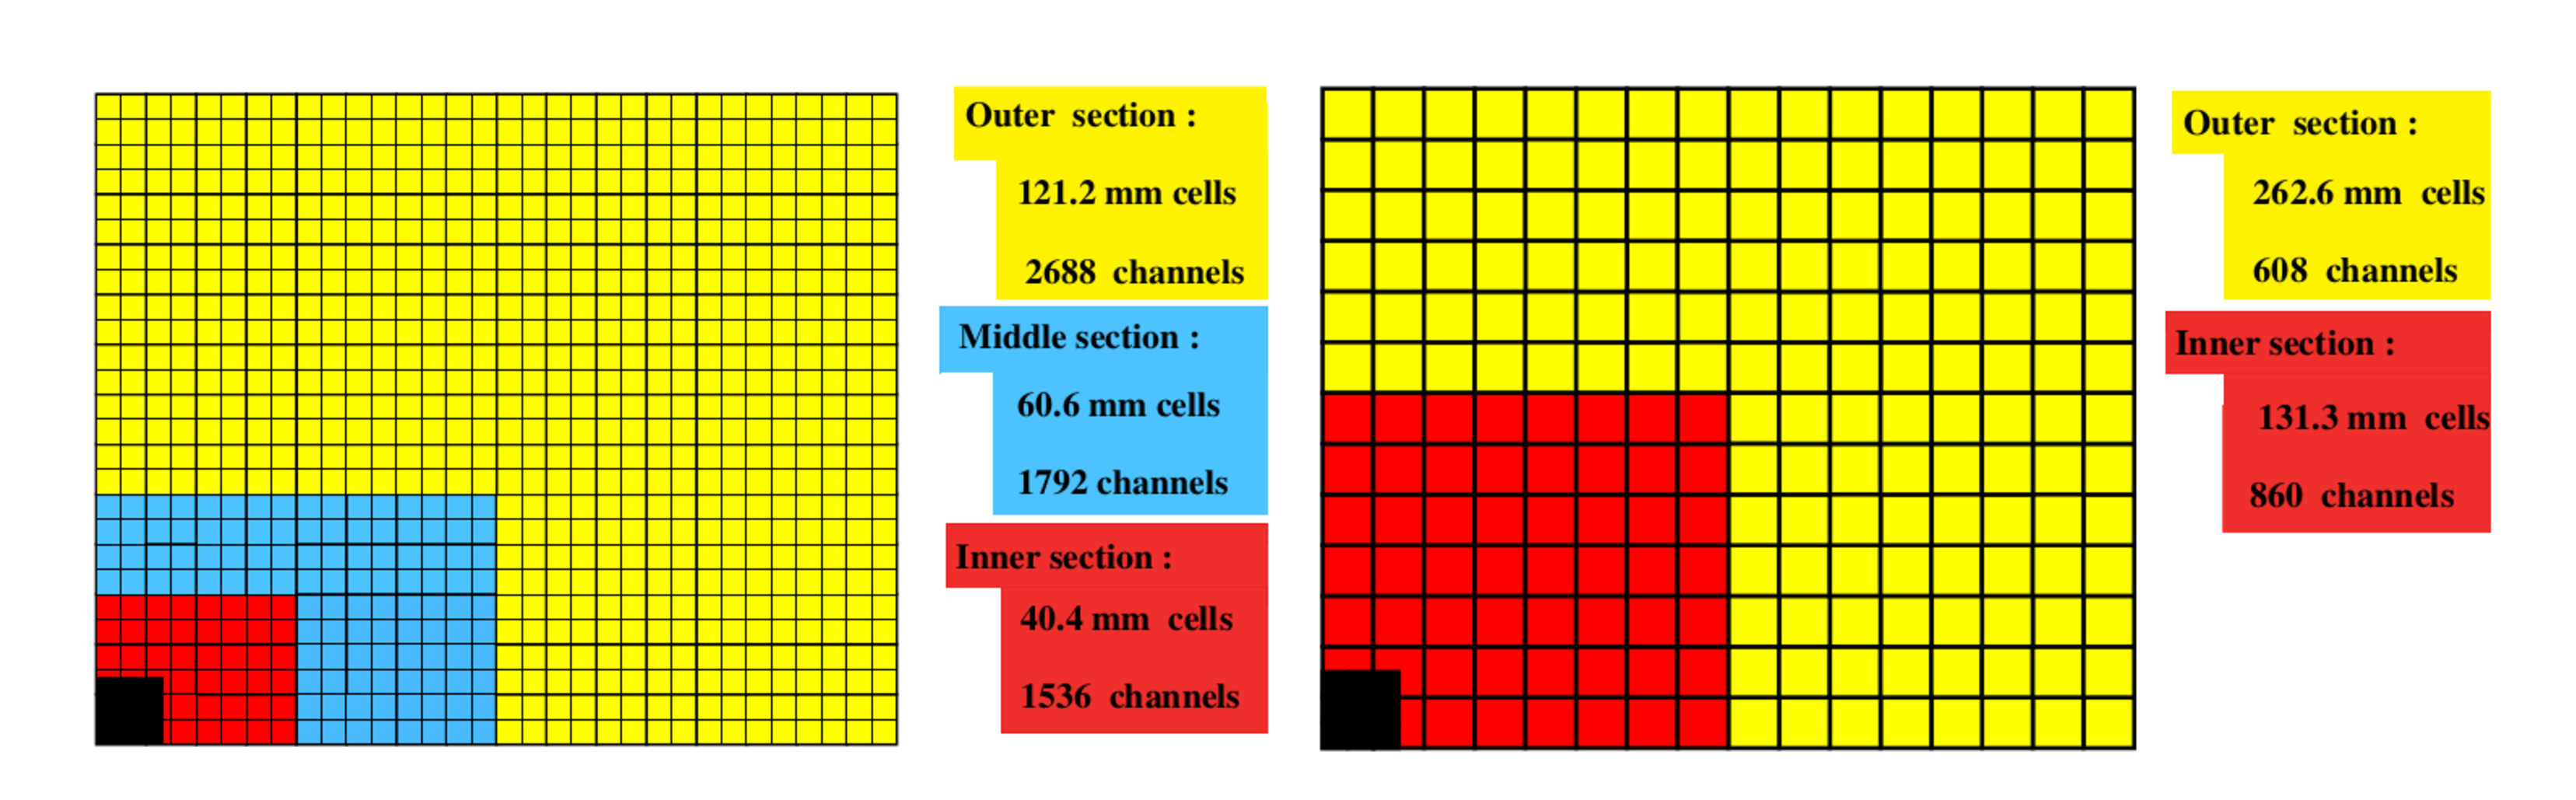
\includegraphics[width=\linewidth]{figures/detector/calorimeters.pdf}
\caption{Segmentation of the SPD/PS and ECAL (left) and the HCAL (right). One quarter of the detector face is shown. Reproduced from Ref.~\cite{lhcbdetector2008}.}
\label{calorimeter}
\end{figure}

\section{Muon system}
\label{sec:detector:muon}

The muon system~\cite{LHCb-DP-2013-001,LHCb-DP-2012-002} is designed, together with the calorimeter system, to provide initial information on whether to accept or reject the event to the first level of hardware trigger, described in \sect\ref{sec:detector:trigger}. The muon system is composed of five stations, labelled M1 through to M5, each containing 276 multi-wire proportional chambers (MWPCs), except the inner-most region of M1, subject to the highest level of radiation, contains 12 gas electron multiplier (GEM) detectors. Station M1 is located upstream from the calorimeters and is only used in the first level of trigger. Stations M2 - M5, located downstream from the calorimeters, are interleaved with 80~\cm thick iron absorbers and are designed to identify and trace penetrating muons. For each muon station the segmentation size increases moving outwards from the beam pipe in four distinct regions, such that each region is subject to the same particle flux. The total active area of the muon system is 435~\ma. Muons with momenta greater than 6~\gevc will typically traverse all five stations. The five stations together have a depth corresponding to 20 interaction lengths. 

Part of the first level of trigger involves performing a stand-alone muon track reconstruction, which requires hits in all 5 muon stations and a calculation of the transverse momentum, \pt, of the tracks. Stations M1 to M3 have the best spatial resolution, which is used to find a rough, fast measurement of the muon \pt for use in the first level of the trigger. Stations M1 to M3 measure muon transverse momentum with a resolution of $\sim$20\%. The muon system provides muon identification for trigger and offline reconstruction with an efficiency larger than 95\%~\cite{LHCb-DP-2014-002}.

\section{Trigger system}
\label{sec:detector:trigger}

The \lhc bunch crossing rate is nominally 40MHz, however there is insufficient processing power to read out the full detector and write every event to storage at this frequency. A dedicated trigger system~\cite{LHCb-DP-2012-004} is therefore implemented to retain interesting events while discarding background events. Triggering occurs in two stages: the low-level hardware trigger using momentum and transverse momentum discrimination, called the Level-0 (L0) trigger, and the high-level software trigger reconstructing the full event, including tracks, called the High Level trigger (HLT). The L0 trigger operates at the bunch crossing rate of 40MHz, reducing the event rate to 1MHz. The HLT only processes events that have passed L0, accepting events at a rate of 5kHz in 2012 (3kHz in 2011). The increase in computing resources in \runtwo meant that events pass HLT and are read out to storage at a rate of 12.5kHz.

A sequence of reconstruction algorithms and thresholds defined in the trigger to select a specific decay is called a trigger line, which returns an accept or reject decision. An event is retained only if it passes at least one trigger line in both L0 and HLT.

\subsection{Level-0 trigger}

The L0 trigger only uses information that can be quickly read out from the calorimeter or muon systems, reducing the event rate from 40MHz to 1MHz, and on an L0 accept the full detector is read out. The L0 trigger relies on the fact that the decay products of \B mesons typically have high transverse momenta due to the large \B mass. The L0 trigger selects high transverse energy clusters in the calorimeters resulting from hadrons, photons and electrons, and high transverse momentum muons in the muon system. The trigger also requires a maximum number of SPD hits to reject high multiplicity events which would use excessive processing time in the HLT. 

The trigger creates {\tt L0Hadron}, {\tt L0Photon} or {\tt L0Electron} candidates depending on which calorimeter subsystem the energy has been deposited in. Events containing at least one candidate above a fixed threshold in transverse energy ({\tt L0Global} candidates) are accepted by the L0 trigger. The hadron trigger selects events with transverse energy, \et $>$ 3.68\gev deposited in the hadronic calorimeter, whereas the electron and photon trigger selects events with \et $>$ 3\gev deposited in the electromagnetic calorimeter. Candidates for {\tt L0Muon} or {\tt L0DiMuon} are created based on the hits in the muon systems and the transverse momentum of the candidate. For a single muon, the muon candidate must have \pt $>$ 1.76\gev, and for a pair of muons, the product of their transverse momentum must be above 1.6$\gev^2$~\cite{trigger_tim}.

\subsection{High Level Trigger}

Events accepted by the L0 trigger are held in a buffer to be processed by the HLT, which has two stages: HLT1, performing partial event reconstruction, and HLT2, performing full event reconstruction. 

For HLT1, the event rate has been reduced by the L0 trigger to 1MHz, allowing latency for the full detector then to be read out. Tracks in the \velo are reconstructed and are then used to form primary vertices using at least five tracks. \velo tracks are identified that either have a large IP, or tracks that match to hits in the muon chamber. Poor quality \velo tracks are rejected. The muon candidates have the additional requirements of high momentum (above 6\gevc) and reasonable track quality (\chisqndf below 25). \velo tracks that are selected by their IP or as a muon candidate are reconstructed using information from the OT and IT-stations in order to determine their momentum. This process is known as forward tracking. Minimum momentum and transverse momentum constraints are applied to reduce processing time when fitting each reconstructed track using a Kalman-filter-based track fit. Successfully extended \velo tracks selected by their large IP are required to have a track \chisq less than three~\cite{trigger_tim}.

In HLT2, the further reduction in event rate by HLT1 allows forward tracking to be performed on all \velo tracks with $p > 5\gevc$ and $\pt > 0.5\gevc$. The HLT2 trigger includes lines for selecting \bquark-hadron decays, prompt charm decays and muonic decays. A large proportion of the HLT2 bandwidth goes to topological trigger lines, which are specifically designed to target partially reconstructed \bquark-hadron decays. Tracks are combined one-by-one requiring the distance of closest approach (DOCA) to be less than 2mm, reaching a total of two, three or four tracks, resulting in the {\tt HLT2Topo(N)BodyBDTDecision} trigger lines, with $N = 2,3,4$ particles forming the vertex. Selection requirements are imposed on these lines based on a multivariate Boosted Decision Tree (BDT) classifier, which uses the sum of transverse momenta, minimum transverse momenta, invariant mass, corrected mass, DOCA, impact parameter significance and flight distance \chisq. Here corrected mass, $m_{corr}$, is defined as

\begin{equation}
m_{corr} \equiv \sqrt{m^2 + {| \pt^{miss} |}^2} + \pt^{miss} \text{ ,}
\end{equation}
where $\pt^{miss}$ represents the missing momentum in the transverse direction. This quantity allows for the case where not all final state particles are reconstructed. This multivariate selection is where most of the rejection power is achieved.

Events that pass HLT2 are written to storage at an event rate of 3kHz (2011), 5kHz (2012) or 12.5kHz (2015 and 2016). These events subsequently undergo the full alignment, calibration and reconstruction processing.

\section{Reconstruction}

\subsection{Track reconstruction}
\label{sec:detector:tracks}

Track reconstruction algorithms combine information from all hits from different sub-detectors, e.g. \velo, TT, IT and OT, to form tracks. There are five categories for track classification, shown in \fig\ref{tracktypes}:

\begin{figure}[h]
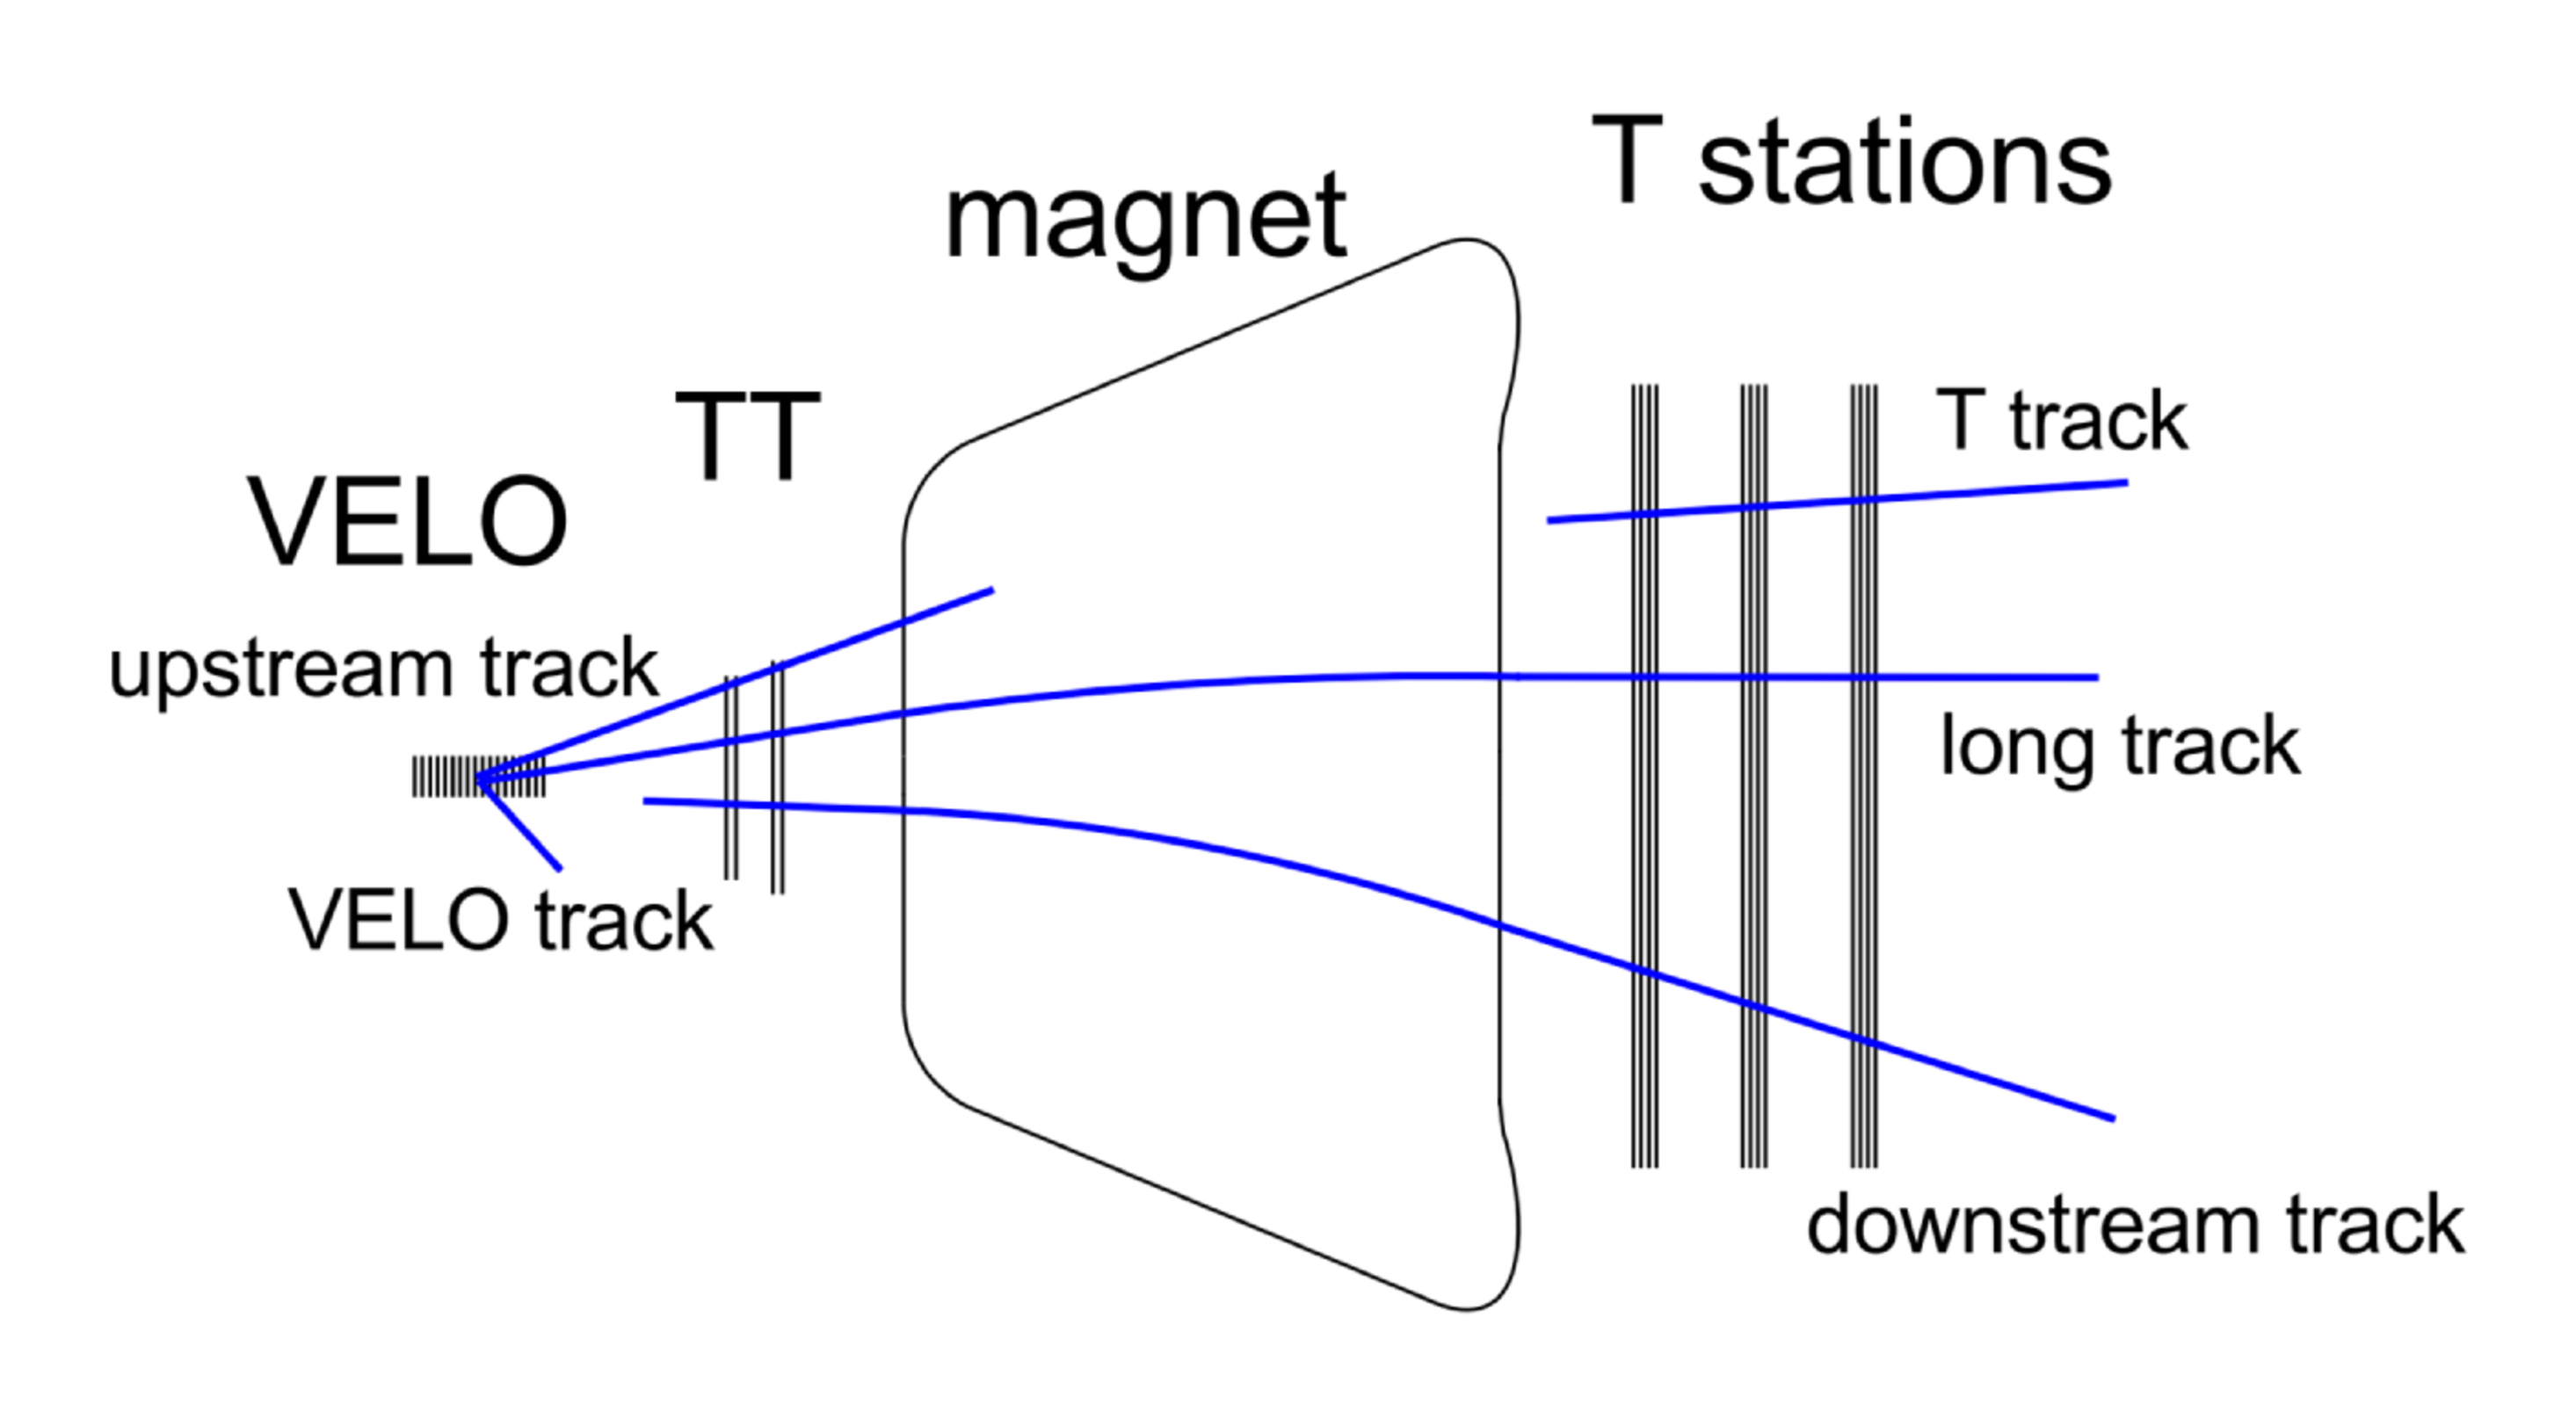
\includegraphics[width=\linewidth]{figures/detector/tracktypes.pdf}
\caption{Schematic diagram of the different tracking sub-detectors (\velo, TT, T-stations) and the different categories of reconstructed tracks (long, downstream, upstream, \velo, T tracks). Reproduced from Ref.~\cite{LHCb-DP-2013-002}.}
\label{tracktypes}
\end{figure}
%1412.6352 figure 14

\begin{itemize}
\item \textbf{Long tracks} traverse the entire tracking system from the \velo to the T-stations. These tracks have the most precise momentum measurement as they have traversed all detector planes and the full magnetic field.
\item \textbf{Downstream tracks} only traverse the TT and T-stations. These tracks are usually a result of long-lived particles, such as \KS mesons, decaying after the \velo.
\item \textbf{Upstream tracks} traverse the \velo and TT stations before being bent out of the detector by the magnetic field due to their lower momentum.
\item \textbf{\velo tracks} leave the \lhcb acceptance after traversing part of the \velo. No momentum information can be obtained from these tracks due to the absence of a magnetic field in this region.
\item \textbf{T tracks} are ones that only have hits in the T-stations. These are typically produced in secondary interactions.
\end{itemize}

Track reconstruction starts with the reconstruction of \velo tracks, which are then propagated through to the TT to determine the particle trajectory. To define a long track, additional hits are searched for in the T-stations that match the particle trajectory. This process finds combinations of clusters in different sub-detectors that are likely to have been formed by a single charged particle travelling though the detector. The sequence of clusters are then fit using a \chisq minimisation procedure with a third order polynomial. Downstream tracks are reconstructed by first searching for T tracks and then finding corresponding hits upstream in the TT by extrapolating the track trajectory back through the magnetic field.

Once the tracks have been identified they are fitted to obtain a best estimate of the track parameters accounting for multiple scattering and energy lost through ionisation. The \chisq of this fit and a neural network classifier are used to reduce the number of fake tracks that are formed by wrongly matching clusters in different sub-detectors, and therefore do not correspond to the passage of a real charged particle.

\subsection{Stripping}
\label{sec:detector:stripping}

The events accepted by the HLT are written to storage. All processing that occurs after this point is known as ``offline'' processing. The events written to storage are processed with more accurate alignment and calibration of the sub-detectors and more sophisticated reconstruction software than HLT. This offline processing stage is referred to in this thesis as ``stripping''. Each family of decays has its own stripping line, which refers to the reconstruction and selection of specified particles in the decay chain of interest. Various loose selection requirements are applied to remove background events to later reduce the processing time and storage requirements. An analysis initially involves taking events returned by the relevant stripping line and developing a more sophisticated selection procedure to further remove background events.

\section{Simulation}

Various simulated samples used in this thesis were generated for signal and background studies. The simulated samples are generated using the \lhcb application \gauss and \boole, which are written using the \gaudi framework~\cite{LHCb-PROC-2011-006,simulation}. \gauss generates particles and their decays as well as simulating the transport of charged and neutral tracks through the detector. \boole is then used to simulate the detector response~\cite{simulation}. 

In the production of simulation samples used for analysis, the first step is the production of \bquark\bquarkbar pairs from $pp$ collisions using \pythia 8~\cite{Sjostrand:2007gs}. One quark in the \bquark\bquarkbar pair is chosen at random to decay via user-specified process and its decay is simulated using \evtgen~\cite{Lange:2001uf}, with \photos~\cite{Golonka:2005pn} modelling any final state radiation. The transport of the decay through the detector is modelled using \geant. \boole then returns the output in the format of real data coming from the front-end electronics. The simulated data are then processed by the trigger, reconstruction and stripping as for real data.

Both magnet polarities, and 2011, 2012, 2015 and 2016 samples are generated with \pythia 8, with all daughter products inside the \lhcb acceptance. Signal samples are simulated \btodkst decays to various \D final states, and with the \Kstarm forced to decay to \KS$\pim$. For the four-body \D final states, the simulated samples are produced assuming the \D decay is uniform over the whole phase space. Various other samples are generated to investigate possible background decays, described in \sect\ref{sec:backgrounds}.

\clearpage
%\begin{savequote}[8cm]
%\textlatin{Neque porro quisquam est qui dolorem ipsum quia dolor sit amet, consectetur, adipisci velit...}
%
%There is no one who loves pain itself, who seeks after it and wants to have it, simply because it is pain...
%  \qauthor{--- Cicero's \textit{de Finibus Bonorum et Malorum}}
%\end{savequote}

\chapter{\label{ch:4-selection}Selection and mass parameterisation of \btodkst decays} 

\minitoc

\section{Selection of \btodkst candidates}
\label{sec:selection}

In this section, the reconstruction and selection procedure for the signal mode, \decay{\Bm}{\D\Kstarm}(\KS\pim) is described, where the particles in brackets refers to the decay products of the proceeding particle. The symbol \D refers to a superposition of \Dz and \Dzb mesons. In this thesis the \Dz meson decays to \Km\pip, \Kp\Km, \pip\pim, \Kp\pim, \Km\pip\pim\pip, \pip\pim\pip\pim and \Kp\pim\pip\pim final states are investigated. The \pim from the \Kstarm decay is referred to as the bachelor particle. The selection is developed for the favoured \kpi mode and then applied with minor alterations to the other \D decay modes. The data analysed in this thesis corresponds to 1\invfb and 2\invfb of $pp$ collisions at $\sqrt{s} = 7\tev \text{ and } 8\tev$ collected in 2011 and 2012 (referred to in this thesis as Run 1), and 1.8\invfb at $\sqrt{s} = 13\tev$ collected in 2015 and 2016 (referred to in this thesis as Run 2).

\subsection{Reconstruction and trigger requirements}
\label{sec:selection:strippingandtrigger}

\decay{\Bm}{\D\Kstarm}(\KS\pim) decays are reconstructed offline and stored in a centrally produced dataset in a stage known as stripping, described in Section \ref{sec:detector:stripping}. At this point of the data-processing chain some loose requirements have been made in order to reduce to the \dataset to a reasonable size for storage. However, the amount of combinatorial background, which is background originating from reconstructing random pion and kaon tracks to form fake \Bm, \Dz, \KS or \Kstarm candidates, is still very high. Therefore further offline selection is applied to candidates passing the stripping and trigger requirements in order to reduce the level of combinatorial background as well as to target specific peaking backgrounds.

The decay is reconstructed starting from the final state particles, and proceeding up the decay chain. In this case, the reconstruction proceeds with \decay{\KS}{\pim\pim}, \decay{\Kstarm}{\KS\pim}, \decay{\Dz}{h^+h'^-} and finally \decay{\Bm}{\D\Kstarm}; at each stage a fit is performing to the parent candidate.

The \KS meson is reconstructed through its decay to two charged pions. Reconstructed tracks can be classified in to different types as described in Section \ref{sec:detector:tracks}. If the pions from the \KS decay leave sufficient hits in the \velo to be included in the track reconstruction they are called long tracks and the reconstructed \KS meson is referred to as LL. Due to the high boost from the $pp$ collision many \KS particles decay outside the \velo. If the pions from the \KS decay do not leave sufficient hits in the \velo, they are called downstream tracks and the reconstructed \KS meson is referred to as DD, with the first hits being recorded in the TT, which typically results in poorer mass resolution. The LL \KS mesons tend to have higher combinatorial background levels as there are many more tracks in the \velo to be misreconstructed compared to further downstream. Due to these difference, the \KS reconstruction types, LL and DD, are treated as separate data samples and a slightly different selection is applied to each.

The \KS candidates are required to have a reconstructed mass within 15 \mevcc of the known mass for LL \KS candidates and within 20\mevcc for DD \KS candidates. The \KS candidate is also required to have a good quality vertex that is well separated from the primary vertex. The \Kstarm candidate is formed from a reconstructed \KS candidate and a \pim candidate, and is required to have a reconstructed mass within 75\mev of the known \Kstarm mass. Similarly the \Dz candidate is reconstructed from the relevant kaon and pion candidates, \eg~in the case of \kpi, a \Km and \pip are reconstructed to form a \Dz candidate, which is required to form a good quality vertex, with a reconstructed mass within 25\mevcc of the known \Dz mass. The \Bm candidate is reconstructed from a \Dz and a \KS candidate forming a good quality vertex. The resulting reconstructed \Bm candidate is required to have a mass in the range 4750 - 5800 \mevcc and an \chisqip $<$ 25, where \chisqip is the difference in the vertex fit \chisq of the PV with and without the particle under consideration. Additionally,there are loose $p$ and \pt threshold requirements on all charged tracks.

The trigger decision for each candidate is categorised as {\tt TOS} (Trigger On Signal) if the particles associated with the signal candidate triggered the event or {\tt TIS} (Trigger Independent of Signal) if other particle produced in the $pp$ interaction, that are not associated with the signal candidate, triggered the event. At the hardware trigger, the \Bm candidates are required to satisfy {\tt L0Hadron TOS} or {\tt L0Global TIS}. At the software trigger level, \Bm candidates are required to satisfy {\tt Hlt1TrackAllL0 TOS} and {\tt Hlt2TopoNBodyBBDT TOS}, where $N = 2,3 \text{ or } 4$. These trigger classifications are described in Section \ref{sec:detector:trigger}.

This analysis uses variables constructed after the entire decay chain has been refitted for all the reconstructed tracks in the decay for each \Bm candidate passing the stripping requirements, with one or more constraints imposed~\cite{Hulsbergen:2005pu}. This procedure improves the resolution of the \Bm mass peak. During this refit, the best fit value of the four-momenta for each particle is found under the given constraints. The \Dz mass and \KS mass are constrained to their known values and the \Bm momentum vector direction is constrained to be parallel to the vector joining the primary vertex (PV) to the \Bm decay vertex. The \Bm mass used in this analysis is constructed for each \Bm candidate by fitting the tracks in the decay with requirements that the \Dz and \KS mass are constrained to their known values and the \Bm momentum vector direction is constrained to be parallel to the vector joining the primary vertex (PV) to the \Bm decay vertex. This results in an improved the \Bm mass resolution.

The offline selection involves imposing requirements on individual variables, such as the reconstructed masses of the intermediate meson states, as well as using a multivariate classifier, and particle identification requirements. The requirements on the masses of the intermediate states reduce the probability of the sample containing \Dz, \KS or \Kstar candidates that do not correspond to a true \Dz, \KS or \Kstar meson state. However, the requirements cannot be too close to the true meson mass as this would result in the removal of a significant proportion of the signal candidates. The signal efficiencies of the \Dz, \KS and \Kstar mass requirements, shown graphically in Figure \ref{masscuts}, are 96\%, 98\% and 82\% respectively. 

\begin{figure}
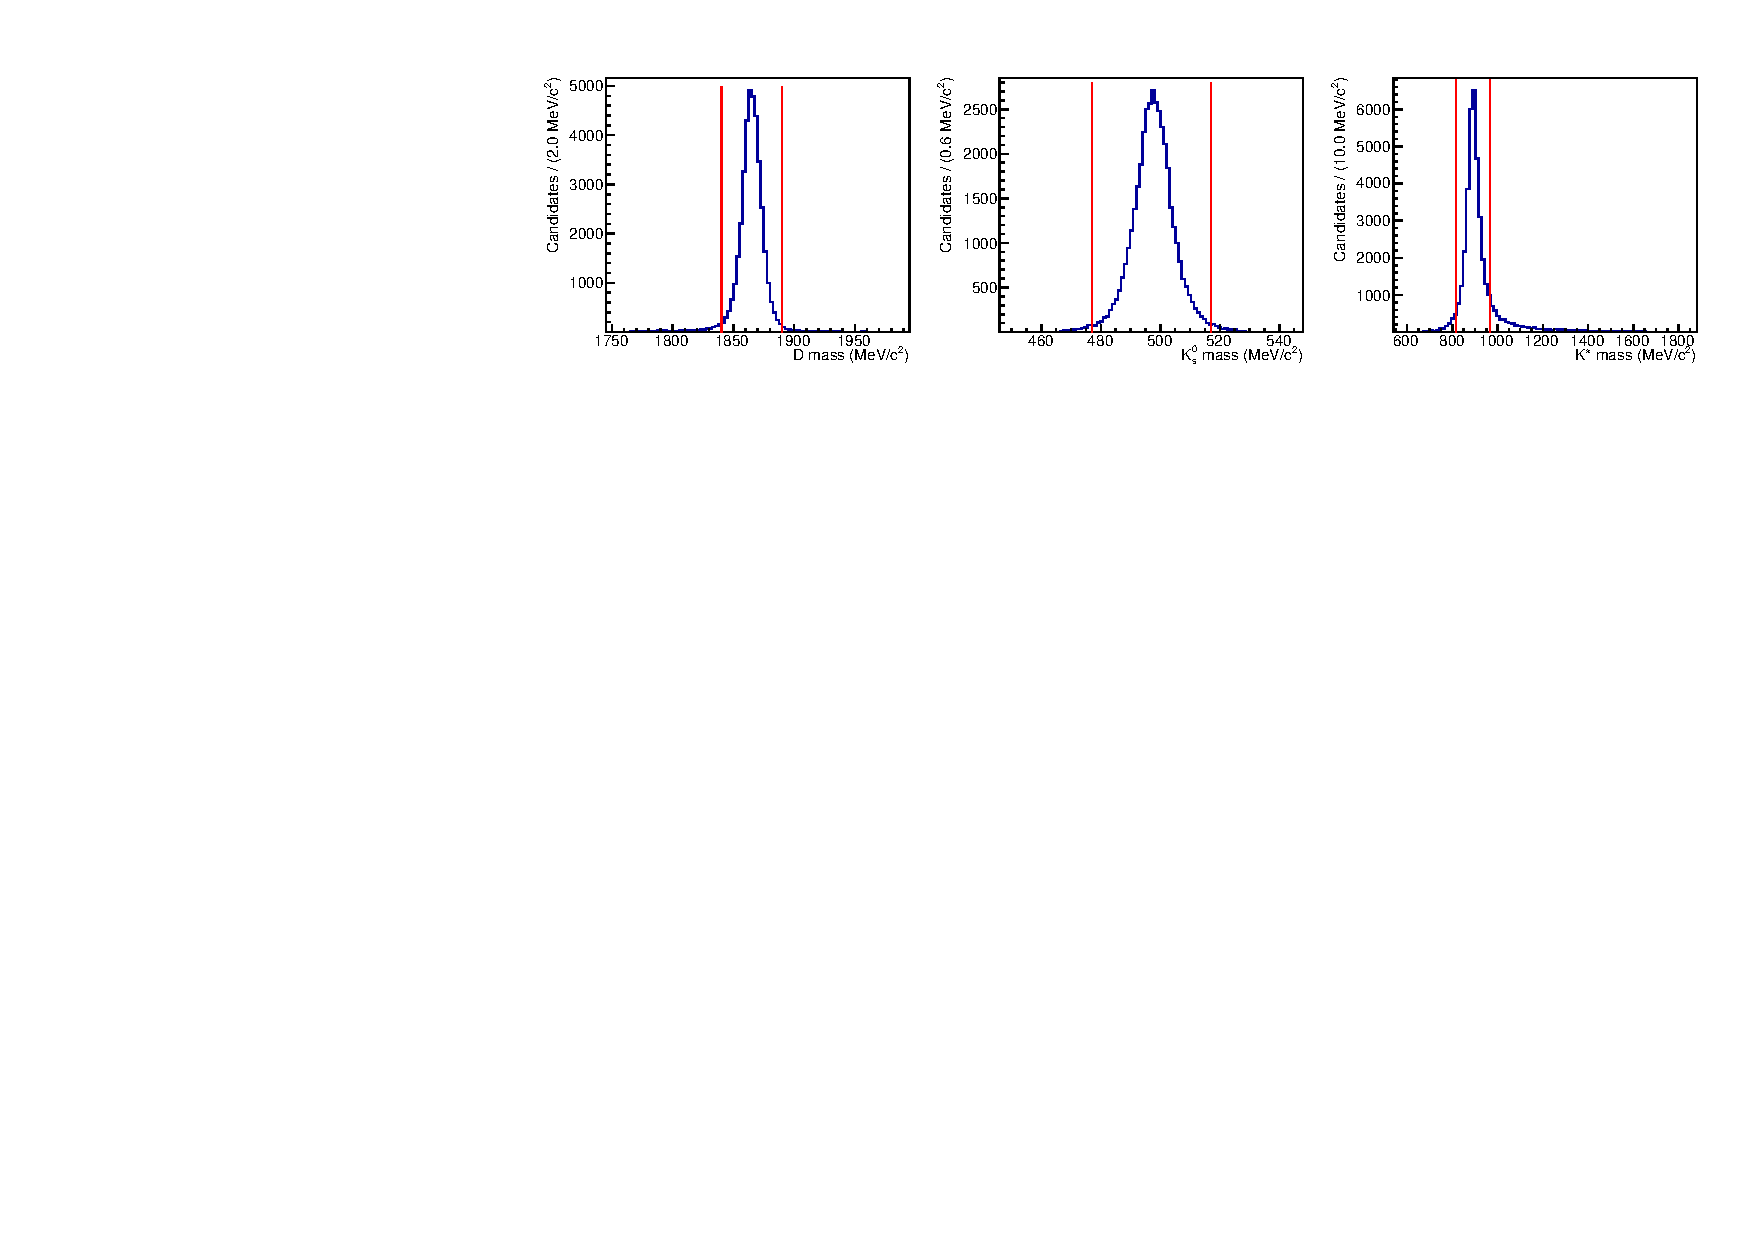
\includegraphics[width=\linewidth]{figures/selection/massDistDD_MC.pdf}
\put(-380,80) {(a)}
\put(-245,80) {(b)}
\put(-110,80) {(c)}
\caption{Distributions from a simulated sample of \kpi DD events of the reconstructed masses for the (a) \Dz, (b) \KS, and (c) \Kstar candidates. The red lines represent the region in recosntructed mass that is accepted as signal in the selection.}
\label{masscuts}
\end{figure}

After the selection described in this section has been applied, the resulting refitted \Bm mass distribution is given in Figure \ref{fig:BmassbeforeBDT}. The signal \Bm mass peak can clearly be observed, however, in order to make accurate measurements of the signal yield in each of the \Dz modes, it is necessary to significantly reduce the combinatorial background. To achieve a much lower combinatorial background, while retaining signal events, requires more sophisticated classification techniques. Additionally, specfic backgrounds must be reduced, and particle identification requirements must be made to reduce the rate of misidentified particles.

\begin{figure}
\centering
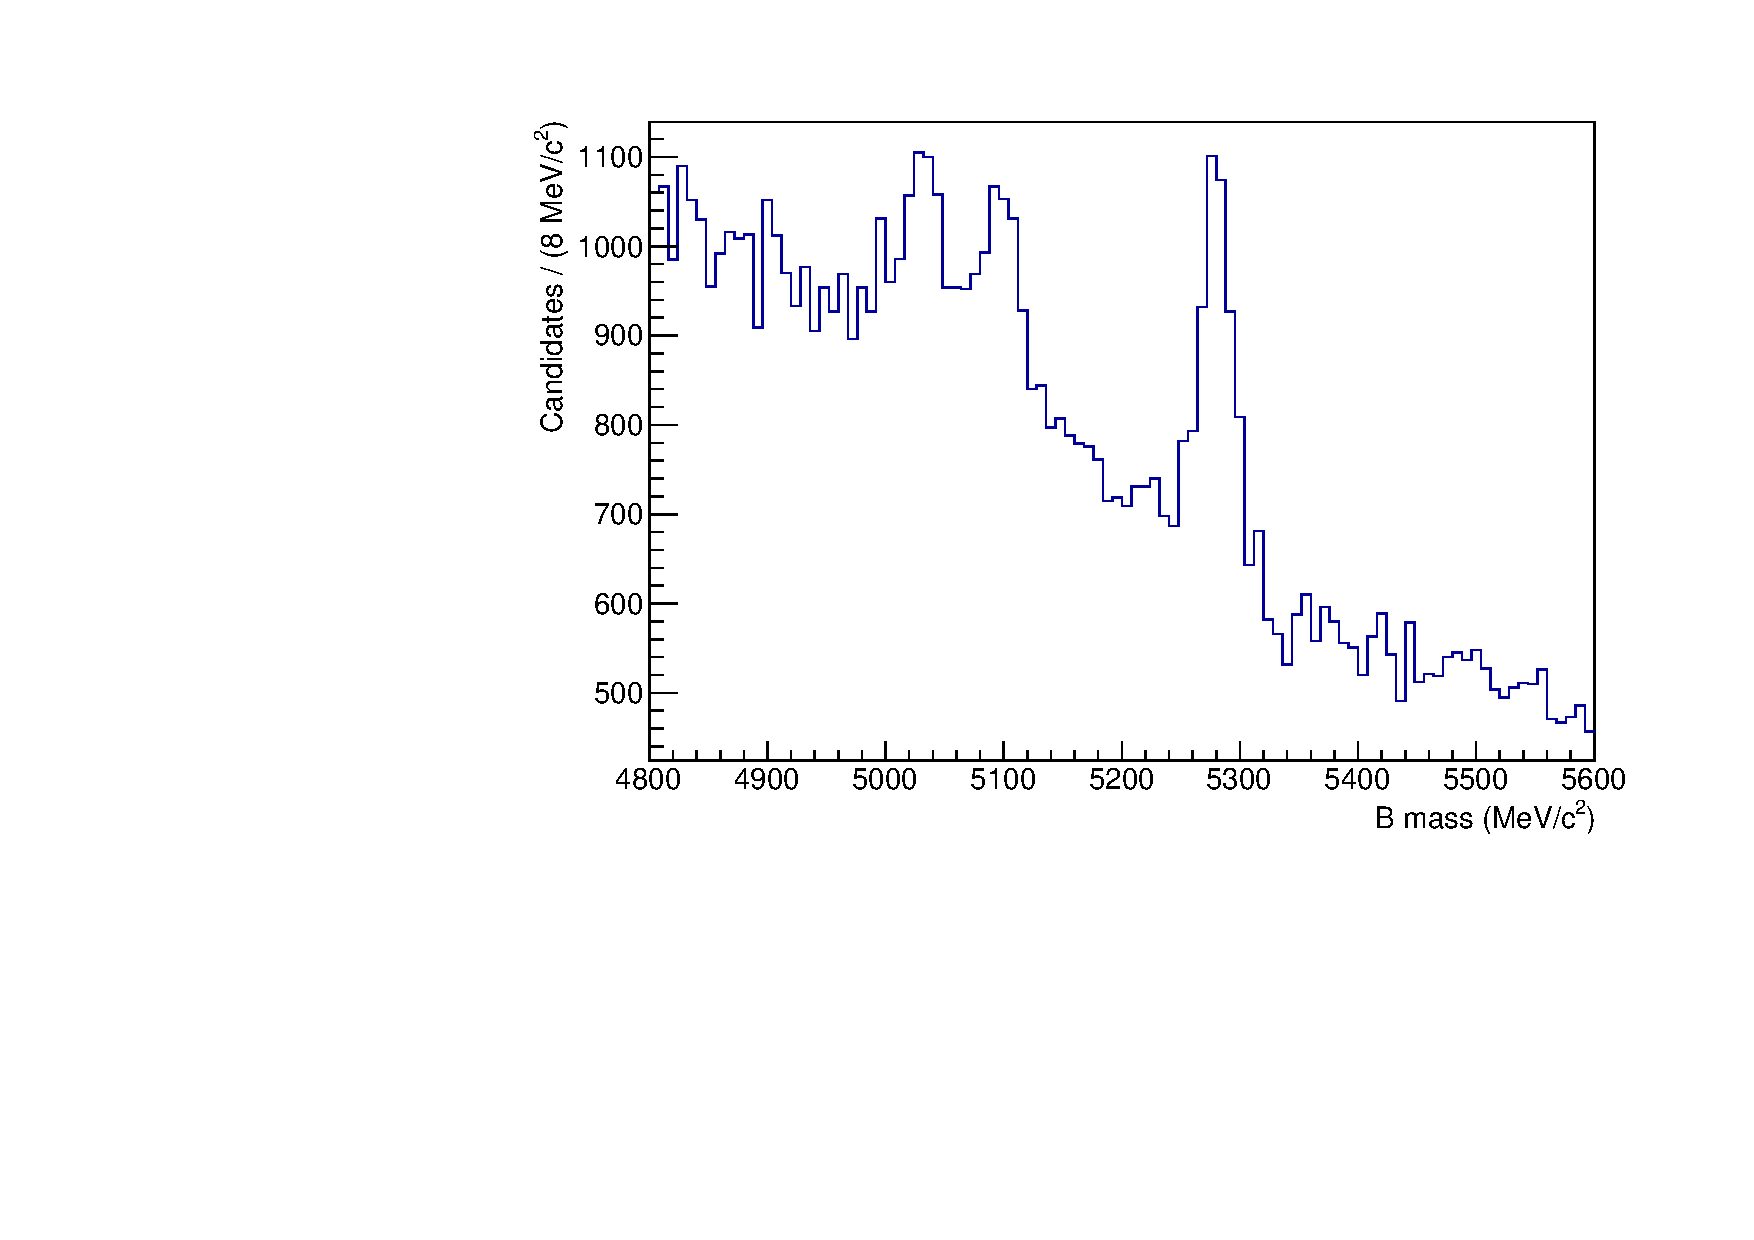
\includegraphics[width=0.6\linewidth]{figures/selection/DataDD_KPi_beforeBDT.pdf}
\caption{The refitted \Bm mass distribution for \kpi DD candidates in \runtwo after the stripping and mass requirements on intermediate states. The \Bm signal peak can be seen at the known \Bm mass (5279 \mevcc) and the peaks at lower reconstructed \Bm mass are discussed later in Section \ref{sec:backgrounds:partreco}.}
\label{fig:BmassbeforeBDT}
\end{figure}


\subsection{Particle identification requirements}
\label{sec:selection:pid}

The selection requirements are almost identical for each of the different \Dz modes, therefore, it is essential to apply PID selection that efficiently distinguishes between pions and kaons. For both the two- and four-body \Dz decays, the supressed \Dz decay modes may have contamination from the most favoured mode, with one or more of the \Dz daughter particles  incorrectly identified. These backgrounds are called crossfeed backgrounds. The ratio of branching fractions for different \Dz decay modes is given in Table \ref{BFdmodes}. The contamination of the most favoured mode is considered as it has the largest branching fraction and therefore would have the largest crossfeed contribution in the other \Dz modes.

\begin{table}[h]
\centering
\begin{tabular}{c|c}
Mode & Branching fraction ratio \\
\hline
\kpi & 1 \\
\kk & 0.10 \\
\pipi & 0.036 \\
\pik & 0.0036 \\
\hline
\hline
\kpipipi & 1 \\
\pipipipi & 0.092 \\
\pikpipi & $-$ 
\end{tabular}
\caption{Branching fractions of the different \Dz decay modes relative to the favoured \kpi mode~\cite{PDG2016}.}
\label{BFdmodes}
\end{table} 

Consider the two-body \Dz decay modes. The suppressed \Dz decay modes may all contain a background from the favoured \kpi mode, where one or more of the \Dz daughters has been incorrectly identified. For example, the \kk mass spectrum may contain background \kpi events, where the \pim is misidentified as a \Km meson. Without PID requirements, these crossfeed backgrounds contribute significantly to the signal. This can be seen in Figure \ref{fig:crossfeed}, which shows the \Dz mass spectrum for the \kk and \pipi data samples both without and with PID requirements applied. Figure \ref{crossfeedkk} (left) contains a \Dz mass peak, but to the right of this there is a second, larger peak, which corresponds to the crossfeed from \kpi events. This peak occurs at higher reconstructed \Dz mass due to the misidentification of the pion as a kaon, which is then added to the invariant mass sum. However, the low mass tail of this large distribution enters into the selected region in \Dz mass, with the selected region illustrated by the red lines. By applying PID requirements on the two \Dz daughter kaons, this crossfeed background can be reduced such that there is negligible contribution within the \Dz mass region selected in this analysis, as shown in Figure \ref{crossfeedkk} (right). 

The same effect is seen in the \pipi mode, illustrated in Figure \ref{crossfeedpipi}. In this case, the crossfeed peak is lower in invariant mass, as a pion is misidentified as a kaon. Also, the crossfeed peak in Figure \ref{crossfeedpipi} (left) is significantly higher than in Figure \ref{crossfeedkk} (left), due to a much lower \decay{\Dz}{\pip\pim} branching fraction, as seen in Table \ref{BFdmodes}.

\begin{figure}
\subfloat[\kk]{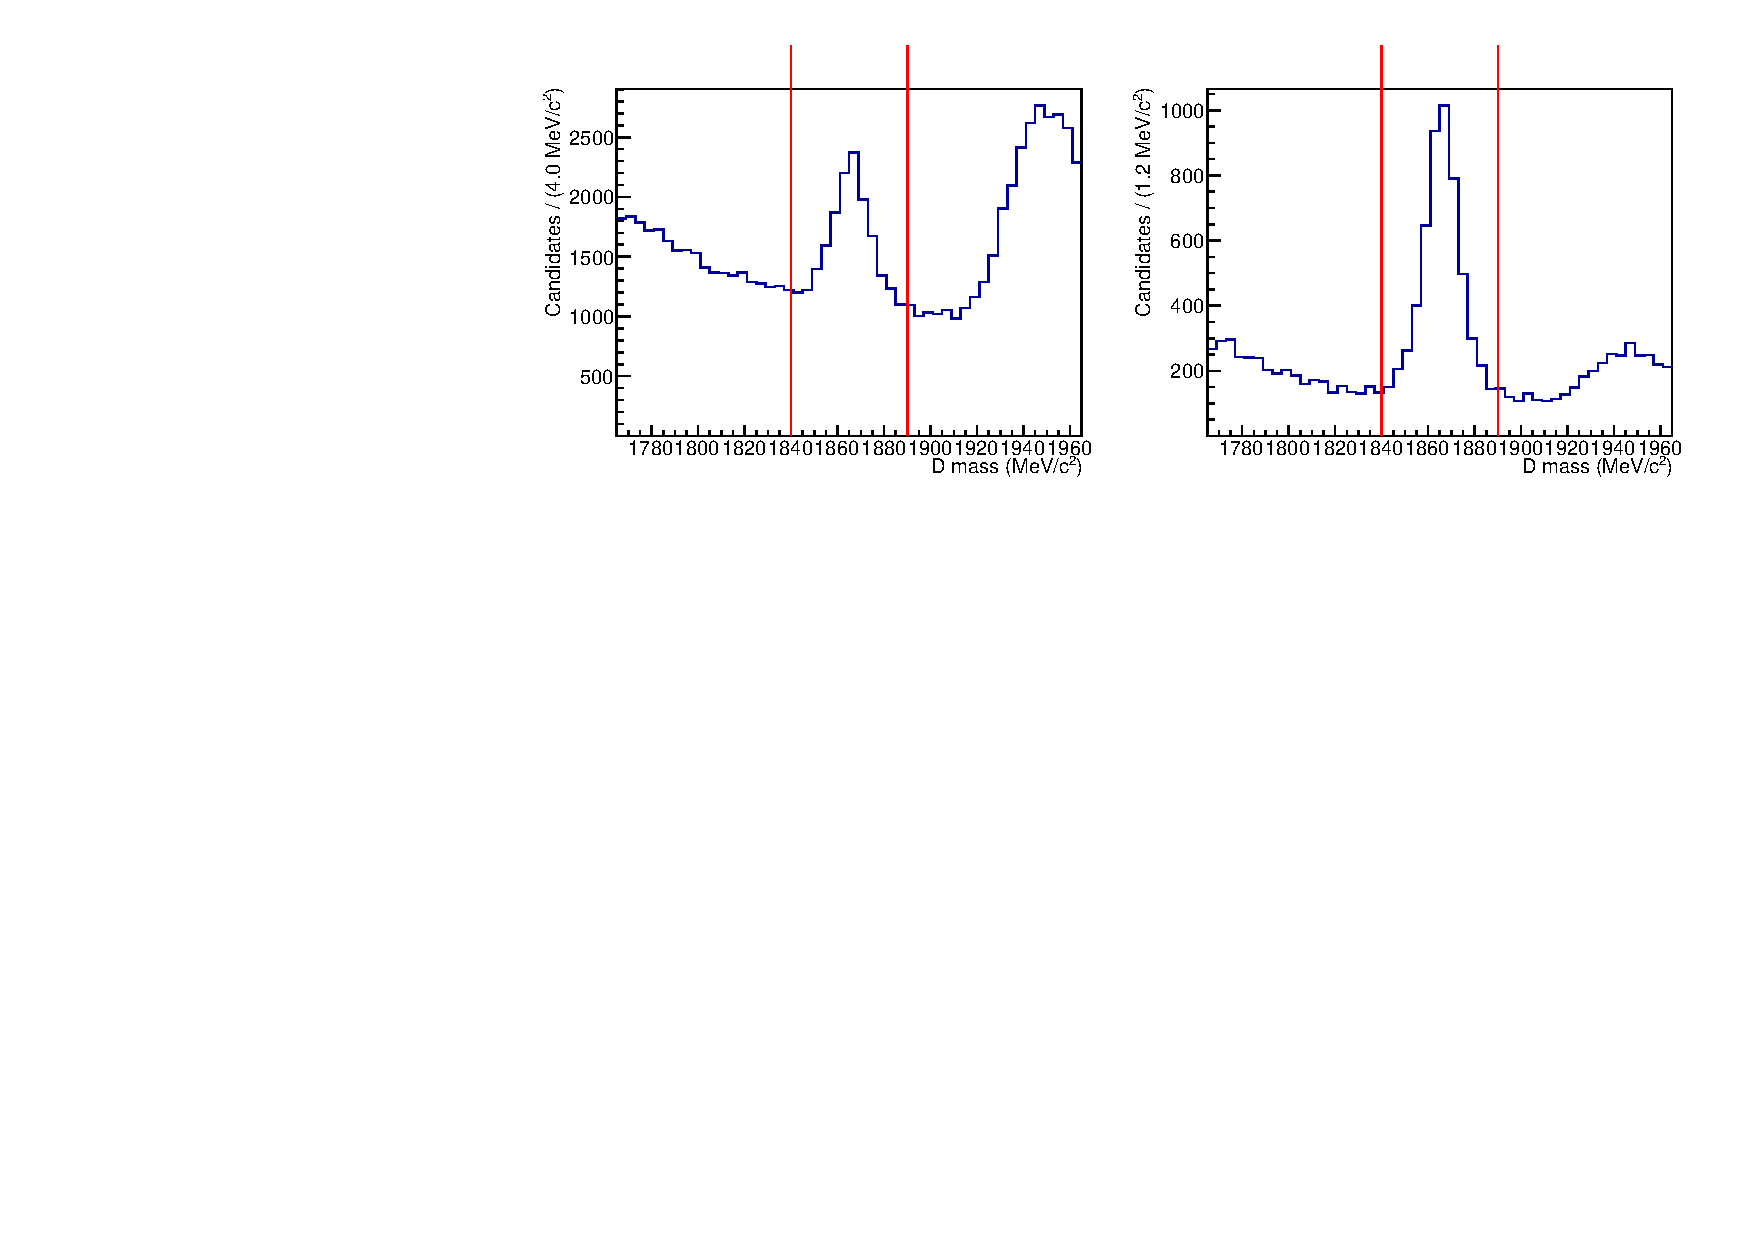
\includegraphics[width=\linewidth]{figures/selection/Dmass_pidcrossfeed_KK.pdf} \label{crossfeedkk}}
\hfill
\subfloat[\pipi]{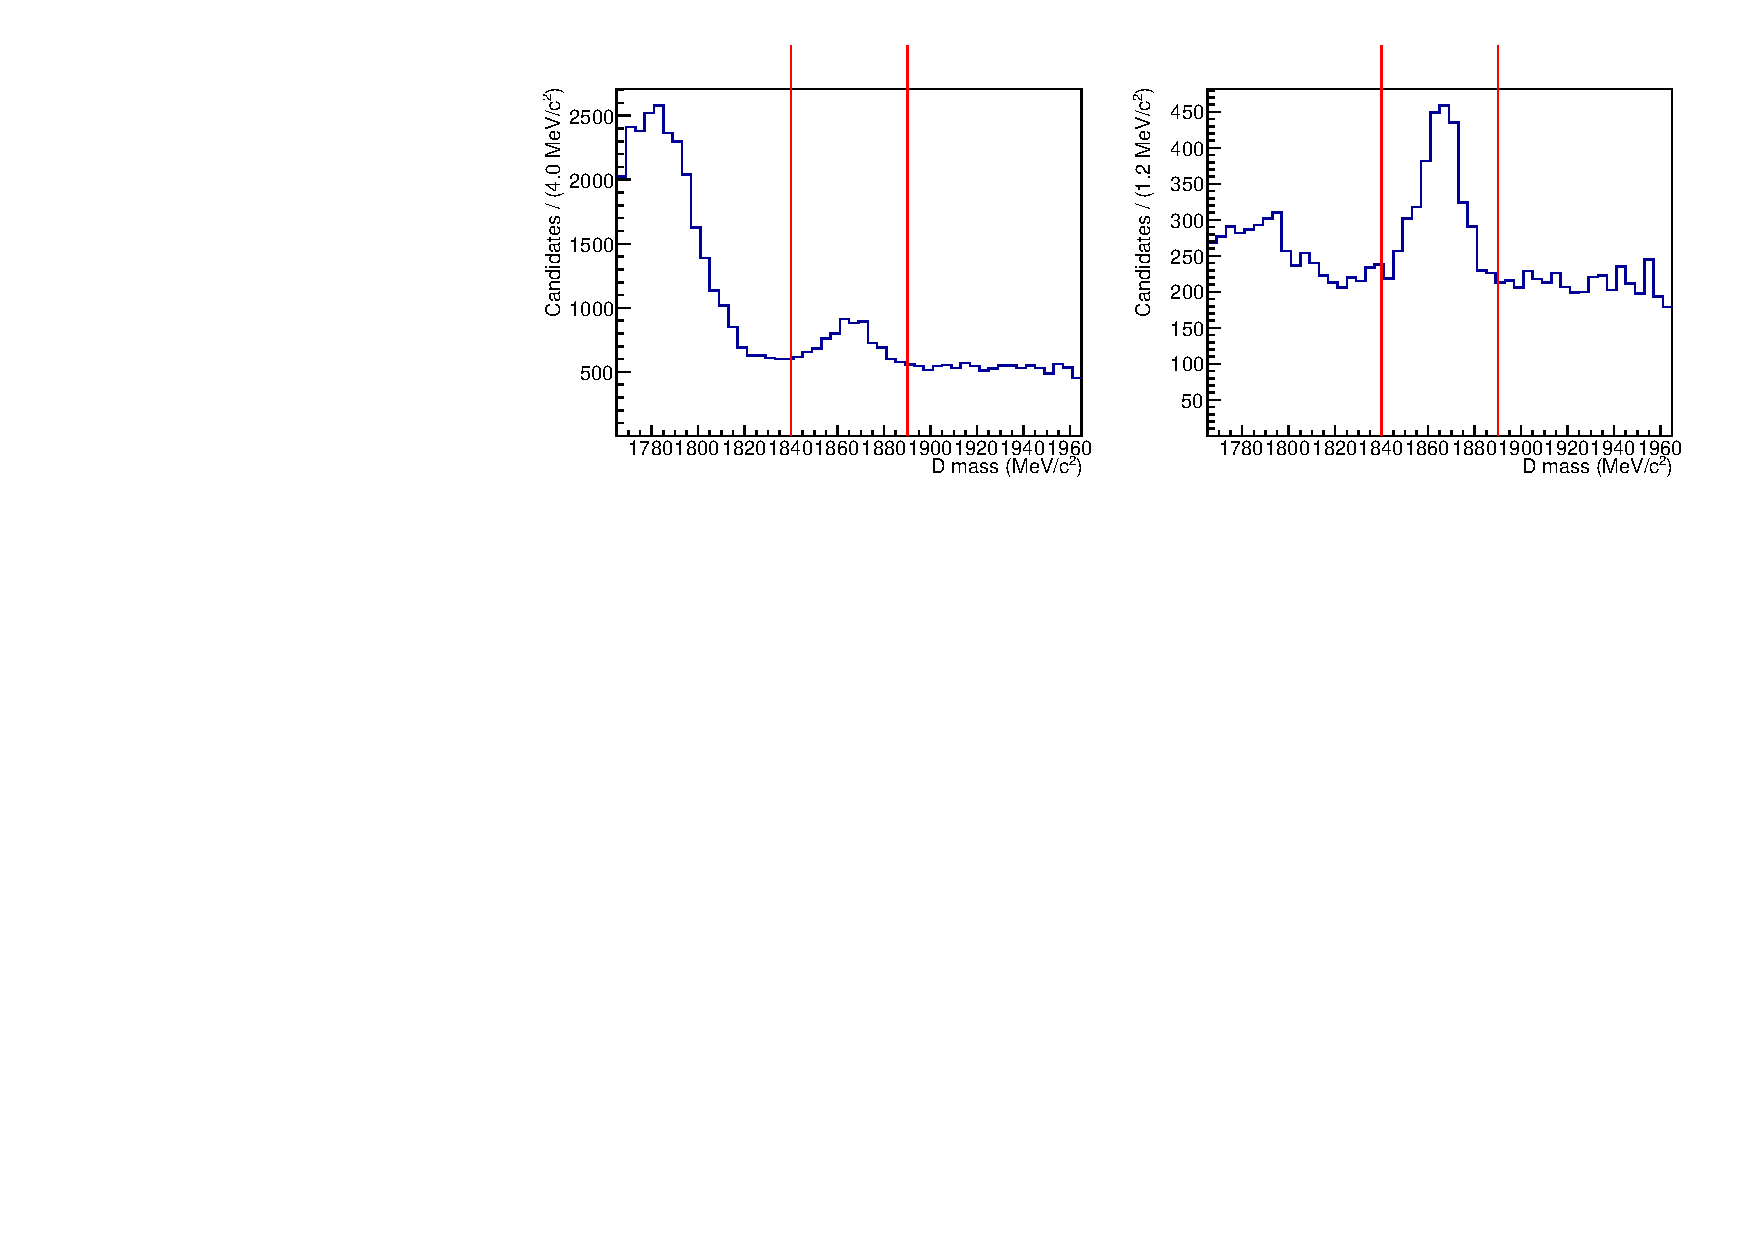
\includegraphics[width=\linewidth]{figures/selection/Dmass_pidcrossfeed_PiPi.pdf} \label{crossfeedpipi}}
\caption{Reconstructed \Dz mass distributions after a prelimiary selection with no PID selection applied (left) and PID selection on the \Dz daughters applied (right), for (a) \kk and (b) \pipi. The red lines indicate the position of the \Dz mass requirement in the selection; events that fall between the red lines are kept as signal events.}
\label{fig:crossfeed}
\end{figure}

The PID requirements on the daughters of the \Dz meson are designed so that no \decay{\Dz}{hh'} candidate can appear in more than one category with a change in mass hypothesis. For the two-body \Dz modes the requirements on the \Dz daughters are: kaons must satisfy DLLK $>$ 2 and pions must satifsfy DLLK $<$ -2, where DLLK is defined in Section \ref{sec:detector:rich}. These requirements have a signal efficiency of 80\% on the \kpi mode, and the probability of incorrect identification of both the kaon and the pion is 0.13\%. This ensures that the probability of misidentification of the \Dz daughters is sufficiently small, such that any crossfeed background is negligible. Crossfeed from \kpi events entering the \pik mass spectrum, would require both \Dz daughters to be misidentified, therefore the resulting reconstructed \Dz mass would not be shifted overall, so fall under the signal \Dz mass peak. This is called the doubly misidentified crossfeed background. In order to reduce this background to negligible levels, the PID requirement cannot be tightened further as this would result in an unacceptable loss of signal. Therefore, a further requirement must be applied to the \pik mode, in addition to the PID requirements discussed. This doubly misidentified crossfeed background, and the steps taken to deal with it, are discussed in detail in Section \ref{sec:backgrounds:crossfeed}.

The same arguments for the two-body \Dz decays modes also apply to the four-body modes. Crossfeed backgrounds may occur in the supressed \Dz modes from misidentified \kpipipi events. Tight PID requirements must be placed on the \Dz daughters in order to reduce these crossfeed backgrounds to negligible levels. For the \decay{\Dz}{\Kmp\pipm\pimp\pipm} modes, e.g. \decay{\Dz}{\Km\pip\pim\pip}, the \Km must satisfy DLLK $>$ 2 and both \pip must satisfy DLLK $<$ -2; no PID requirement is applied for the \pim. These requirements have a signal efficiency of 74\% on the \kpipipi mode, and the probability of incorrect identification of both the \Km and the a \pip is 0.10\%. For the \decay{\Dz}{\pip\pim\pip\pim}, the two \pip mesons must satisfy DLLK $<$ -2 and no PID requirements are placed on the \pim mesons. The doubly misidentified crossfeed background from \kpipipi events in the \pikpipi mode must be investigated further in order to reduce it to negligible levels, as detailed in Section \ref{sec:backgrounds:crossfeed}.

In addition to the correct identification of the \Dz daughters, it is also necessary to consider possible misidentification of the bachelor pion (the pion originating directly from the \Kstarm decay). A PID requirement must be made on this bachelor pion to lower the combinatorial background and reduce the \decay{\Bm}{\D\KS\Km} background to negligible levels. The \decay{\Bm}{\D\KS\Km} background is discussed in more detail in Section \ref{sec:backgrounds:b2dkks}. For all \Dz decay modes, the bachelor pion is required to satisfy DLLK $<$ 4. This requirements has a signal efficiency of 96.4\% when applied to the \kpi mode, and the probability of misidentification of the bachelor pion is 7.9\%. No PID requirements are placed on the \KS daughters as it is not necessary due to the high purity of the \KS meson, described in Section \ref{sec:backgrounds:contamination}. 

The combined efficiency of this PID selection for the \kpi favoured mode is 78\%. The probability of \pik events passing the PID selection for the favoured mode is 0.13\%, i.e. the probability of both \Dz daughters being misidentified. The PID efficiencies are discussed in more detail in Section \ref{sec:cpfit:efficiencies:pid}. 

\subsection{Peaking backgrounds and selection used to supress them}
\label{sec:backgrounds}

There are many backgrounds to be considered where certain particles in the decay chain are missed in the reconstruction process, or incorrectly identified. These effects can result in backgrounds that form peaking structures in the \Bm mass spectrum, which are dangerous if they significantly affect the \Bm mass spectrum. These backgrounds must either be reduced to negligible levels using targeted selection choices, or correctly modelled and included in the fit to the invariant \Bm mass spectrum. This section discusses each of the peaking backgrounds individually and the strategy employed to deal with them.

\subsubsection{Partially reconstructed \boldmath$B \to D^*K^*$ decays}
\label{sec:backgrounds:partreco}

The main class of backgrounds in this analysis is the partially reconstructed \decay{\B}{\Dstar\Kstar} decays, including \decay{\Bm}{(\decay{\Dstarz}{\Dz[\piz]})\Kstarm}, \decay{\Bm}{(\decay{\Dstarz}{\Dz[\gamma]})\Kstarm} and \decay{\Bd}{(\decay{\Dstarp}{\Dz[\pip]})\Kstarm}, where the particle in square brackets in not reconstructed. As each of these backgrounds involves a pion or photon being missed in the reconstruction, the reconstructed \Bm mass for these backgrounds appears below the signal peak. This background is irreducible as it is very similar to the signal, therefore these partially reconstructed backgrounds are modelled and included as components in the fit to the \Bm mass spectrum, which is discussed in detail in Section \ref{sec:massfit:partreco}.

\subsubsection{Backgrounds of type to \boldmath$B \to K^*hh'$ decays}
\label{sec:backgrounds:charmless}

Backgrounds that involve the same final state particles, but do not proceed via one of the intermediate state particles are very important, as they peak in the same region of \Bm mass as the signal. These backgrounds need to be properly understood and reduced to negligible levels such that they do not incorrectly contribute to the estimate of the signal yield. 

Charmless backgrounds are classified as \Bm meson decays that do not proceed via a \Dz meson. This is a peaking background under the signal region which is expected to be uniform in \Dz mass. The variable used to investigate this background is the flight distance significance (FD) of the \Dz in the $z$ direction. The FD significance a particle $X$ is defined as, 
\begin{equation}
\text{FD significance} = \frac{z_X - z_B}{\sqrt{\sigma_X^2 + \sigma_B^2}}
\label{FDdefinition}
\end{equation}
where $z_{X,B}$ is the $z$ position of the decay vertex of the $X,B$ particle and $\sigma_{X,B}$ is the uncertainty in the $z$ position of the $X,B$ decay vertex.

By requiring the \Dz to have a larger FD significance, it increases the probability that the events in the sample contain a true \Dz meson. The charmless background is estimated by investigating the \Bm mass distribution of the candidates in the data sample that have a reconstructed \Dz mass greater than 50 \mevcc away from the nominal \Dz mass, and is therefore very unlikely to contain a true \Dz meson. This region of \Dz mass referred to here as the \Dz mass sidebands, which are illustrated in Figure \ref{Dsidebands}.

\begin{figure}
\centering
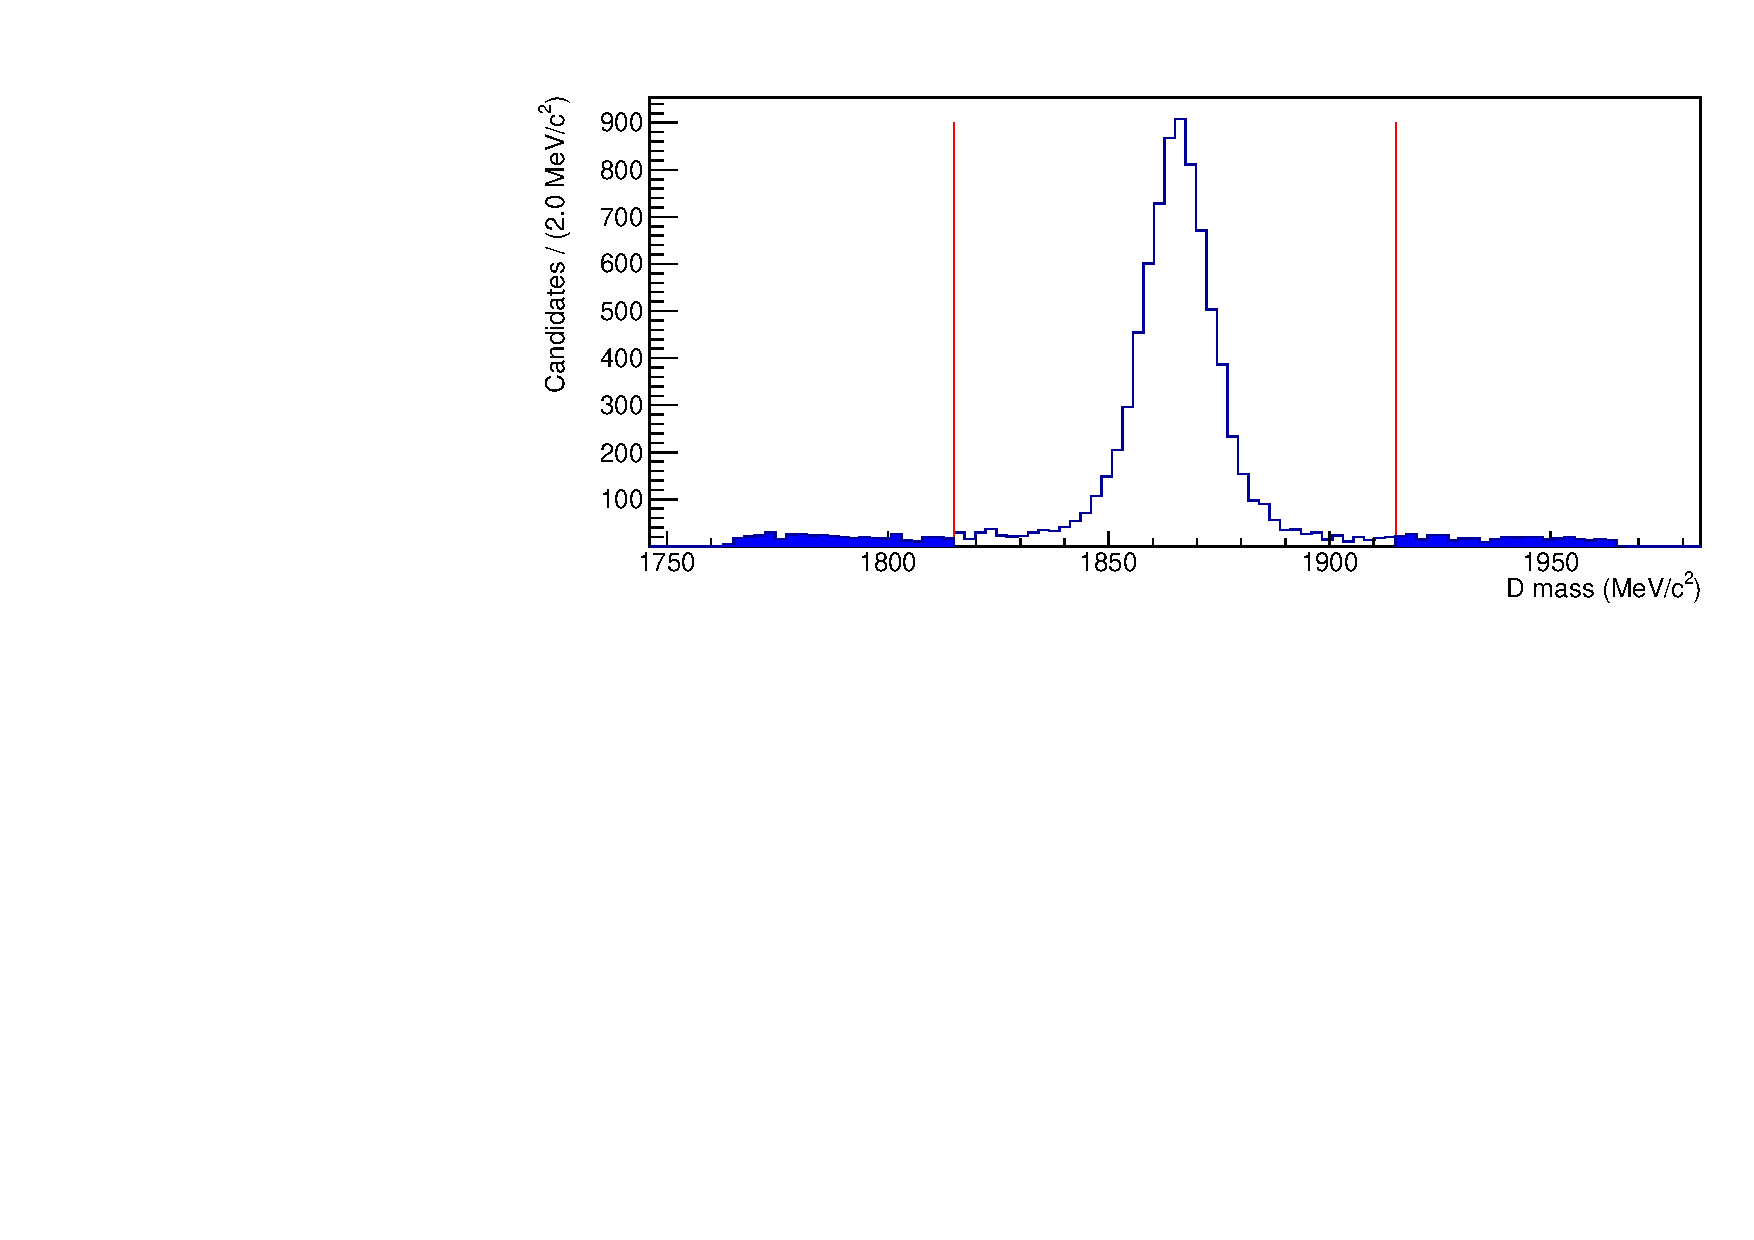
\includegraphics[width=0.8\linewidth]{figures/backgrounds/Dsidebands.pdf}
\caption{Reconstructed \Dz mass for \kpi DD candidates with \runone and \runtwo samples combined. The red lines indicate the values 50 \mevcc away from the nominal \Dz mass, and the bins shaded in blue represent the events that contribute to the \Dz mass sidebands, These events are expected to be dominated by charmless decays, and so are subsequently plotted in \Bm mass to investigate the charmless contribution.}
\label{Dsidebands}
\end{figure}

A simple fit is performed to the invariant \B mass distribution, formed from the data in the \Dz mass sidebands, using a Gaussian to model the signal and an exponential shape to model the background. Variables that have been refitted with constraints, including the constraint that the \Dz is fixed to its known mass, are used in the selection, which favours events towards the true \Dz mass. This effectively removes the \Dz sidebands and therefore the charmless background cannot be estimated. In order to correctly estimate the background contribution in the \Dz mass sidebands, a modified selection is applied with the refitted vertex \chisq replaced with the vertex \chisq with no refit applied. For each \Dz decay mode, two fits are performed on data, one requiring the \Dz FD significance to be greater than zero and the other requiring it to be greater than 2$\sigma$, as shown in Figure \ref{charmlesspipi} for \pipi.

\begin{figure}
\centering
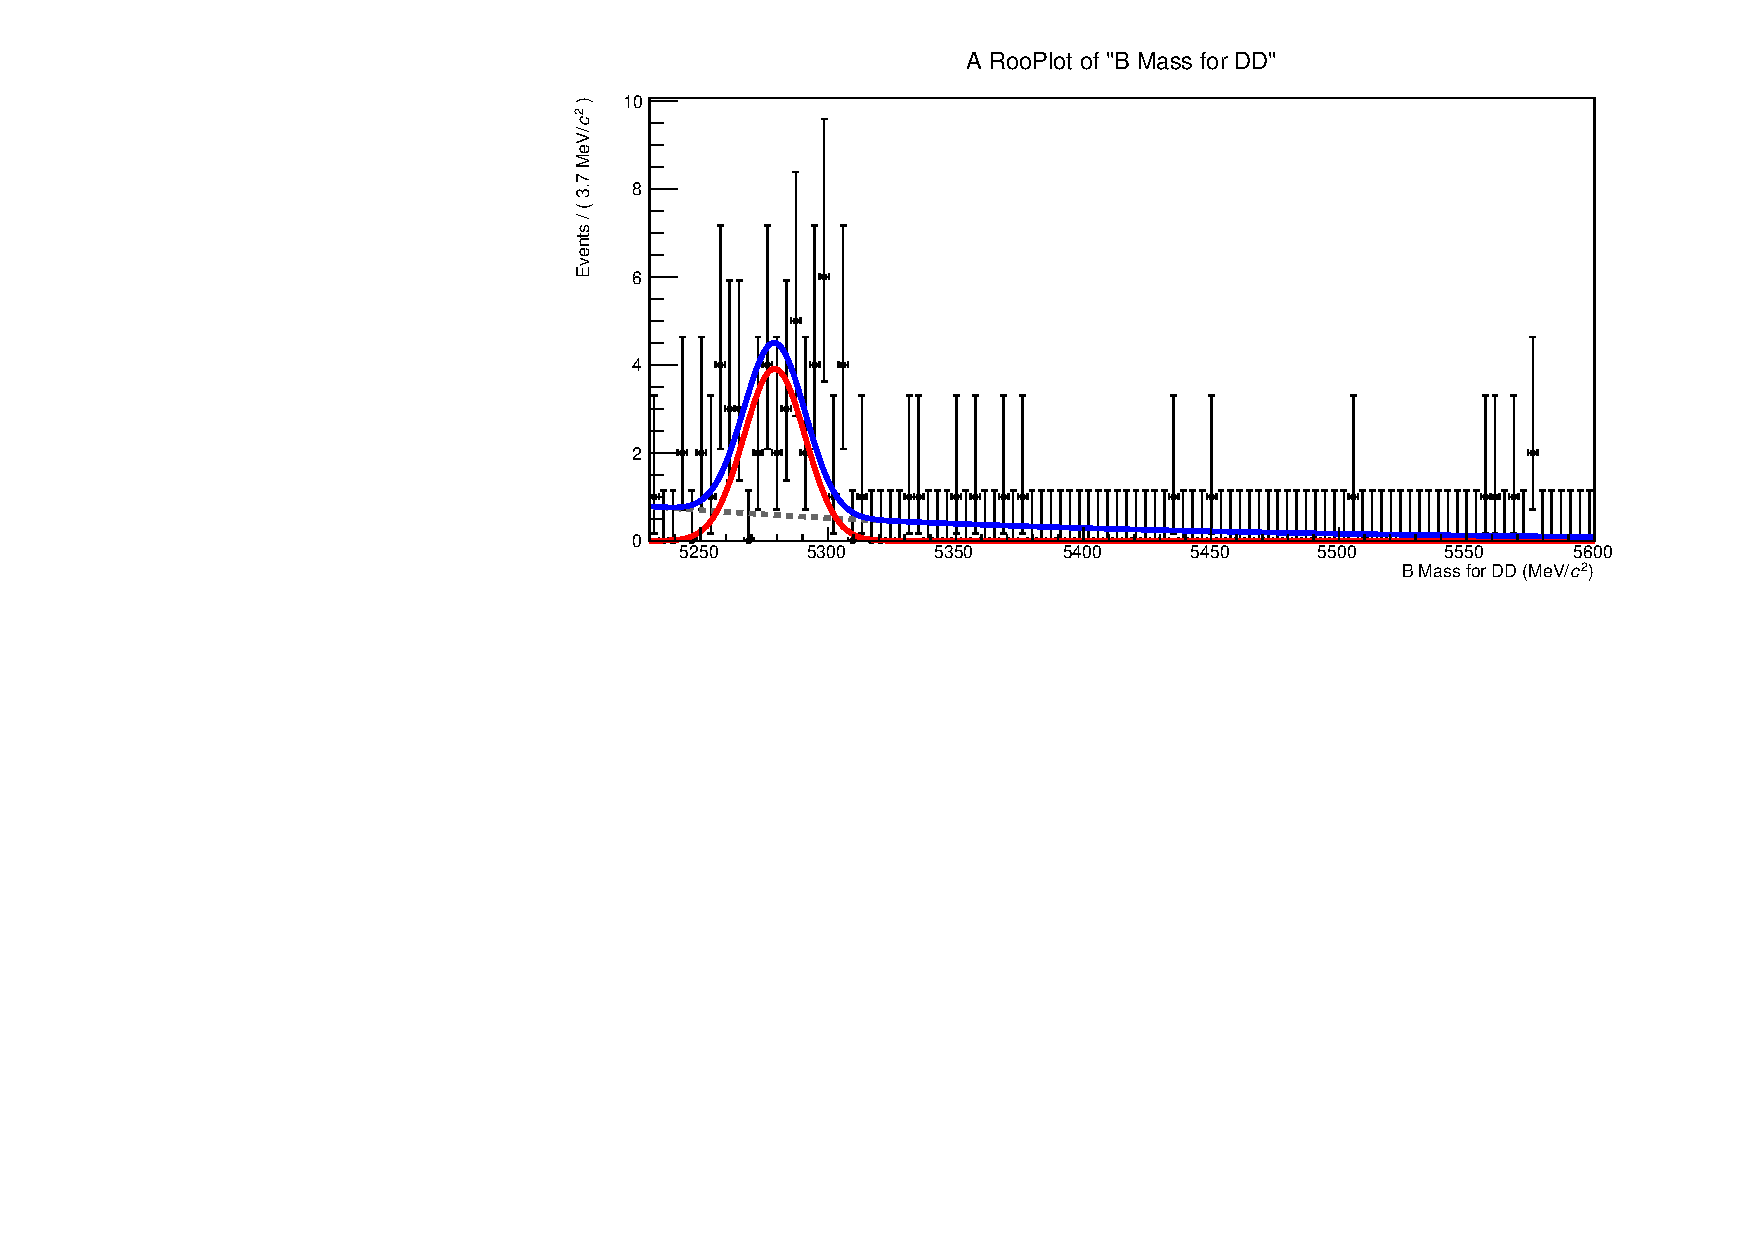
\includegraphics[width=0.7\linewidth]{figures/backgrounds/charmlessFit_PiPi_DD_FD0.pdf}
\put(-100,100) {(a)}
\hfill
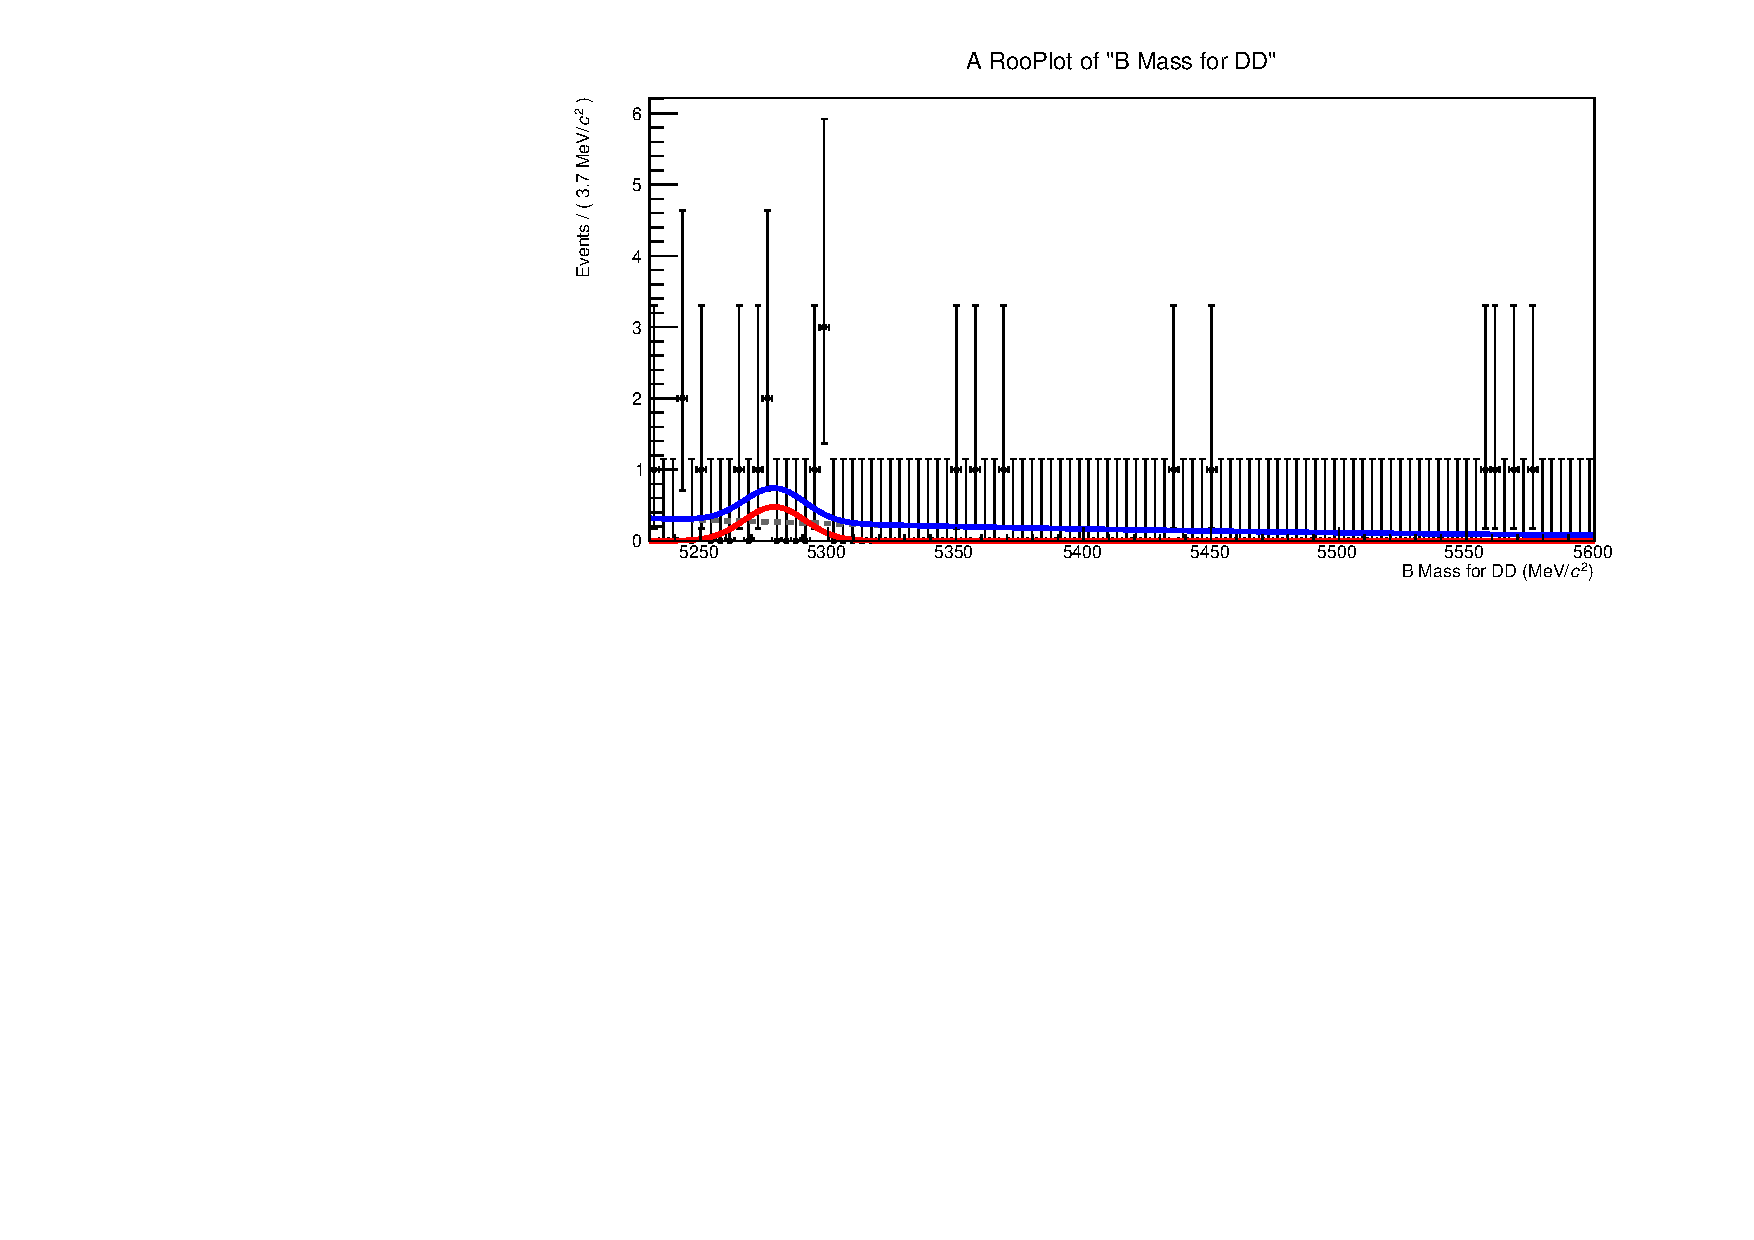
\includegraphics[width=0.7\linewidth]{figures/backgrounds/charmlessFit_PiPi_DD_FD2.pdf}
\put(-100,100) {(b)}
\caption{Fits, using the Run 1 data, to the refitted B mass taking \pipi candidates from the \Dz mass sidebands after requiring the FD significance to be (a) greater than 0 and (b) greater than 2$\sigma$. A Gaussian is used to model the signal and an exponential for the combinatorial background.}
\label{charmlesspipi}
\end{figure}

These fits give the yield of the \Bm mass peak in the \Dz mass sidebands, which are subsequently scaled to provide an estimate for this background within the \Dz mass window. By being able to quantify the number of charmless events expected in the \Bm mass spectrum after a given selection, it is possible to determine if the charmless background has been reduced to negligible levels. 

In the final selection, the \Dz FD significance is required to exceed 2$\sigma$, as all charmless contributions are consistent with zero under this requirement, while retaining 72\% of the signal events. The expected yields in most of the two- and four-body \Dz decay modes are significantly less than 1\% of the signal yield and are therefore considered negligible. However, the estimated charmless contribution in the \pipi mode is greater than 1\% and so could affect the results. The \Dz FD significance requirement is not tightened further for the \pipi mode, as this would results in an extra 10\% loss in signal events, which is deemed unacceptable. Instead the possible charmless contribution in the \pipi mode is considered as a source of systematic uncertainty, details are given in Section \ref{sec:systematics}. 

\subsubsection{\boldmath \decay{\Bm}{\D\pim\pip\pim}}
\label{sec:backgrounds:b2dpipipi}

Having considered backgrounds without the \Dz meson present, we now consider backgrounds that do not occur via a \KS meson. These \decay{\Bm}{\D\pim\pip\pim} decays, with a branching fraction of $5.7 \times 10^{-3}$~\cite{PDG2014} (about 50 times the signal \decay{\Bm}{\D\Kstarm(\KS(\pip\pim)\pim)} branching fraction), are expected to occur as a peaking background underneath the signal. In order to remove this background, events are selected with the requirement that the \KS has travelled within the detector. For DD candidates this requirement is already satisfied, however for LL candidates a minimum requirement on the flight distance significance of the \KS in the z direction, defined in Equation \ref{FDdefinition}, is used to remove this background. 

The \decay{\Bm}{\D\pim\pip\pim} background is estimated by taking the \KS mass sidebands ($>$ 20 MeV from nominal \KS mass) in data and performing a fit to the invariant \Bm mass distribution, as described in Section \ref{sec:backgrounds:charmless}. A Gaussian is used to model the signal and an exponential for the combinatorial background. A modified selection is applied that does not use any DTF variables, as described in Section \ref{sec:backgrounds:charmless}. This fit is performed on \kpi data requiring the \KS FD significance to be greater than zero and 5$\sigma$, as shown in Figure \ref{strangelessfits}. Using these fits the estimated \decay{\Bm}{\D\pim\pip\pim} yield in the signal region with \KS FD significance $>$ 0 is $77 \pm 11$ and with \KS FD significance $>$ 5 is $1.0 \pm 1.0$. For the final selection, the \KS FD significance is required to be greater than 5$\sigma$ as it supresses the \decay{\Bm}{\D\pim\pip\pim} background to a negligible level.


\begin{figure}
\centering
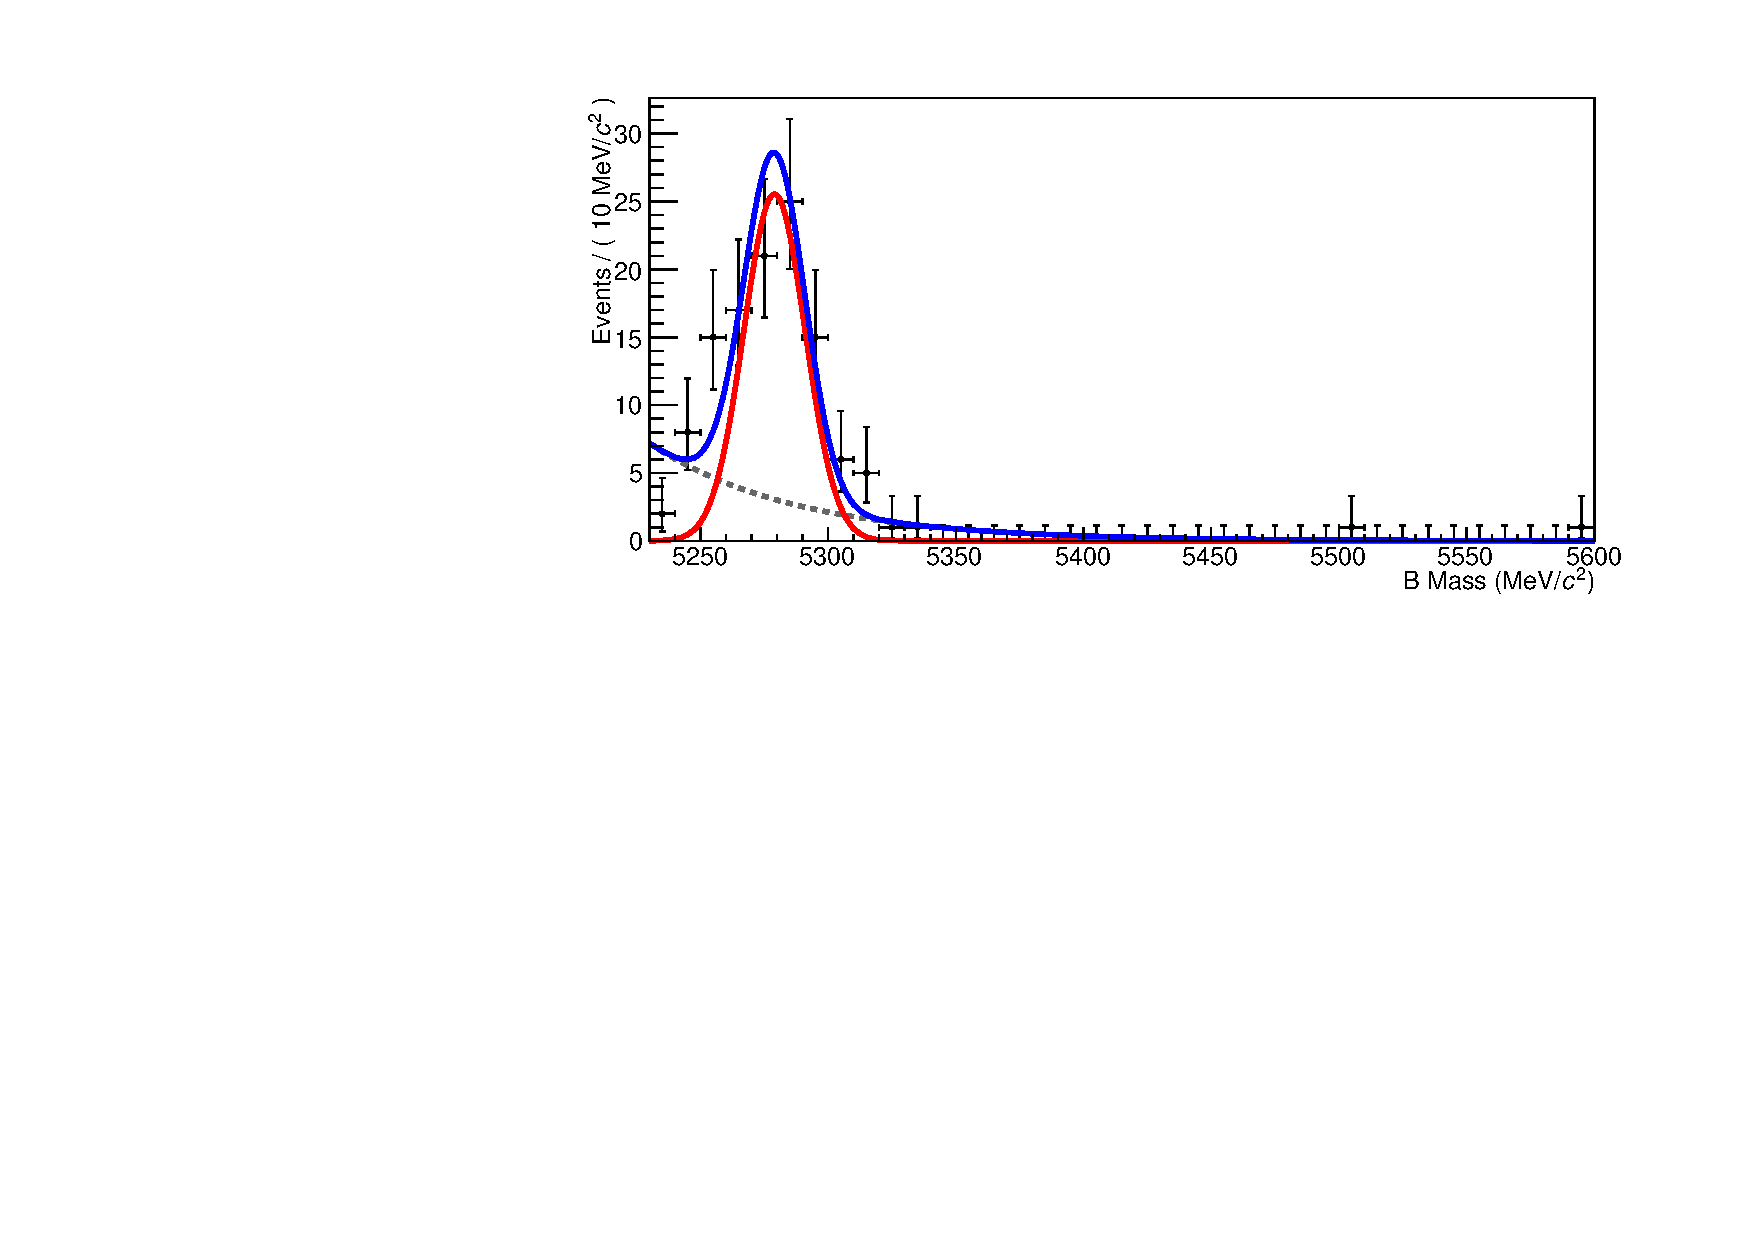
\includegraphics[width=0.7\linewidth]{figures/backgrounds/B2DpipipiFit_KPi_LL_FD0_run2.pdf}
\put(-100,100) {(a)}
\hfill
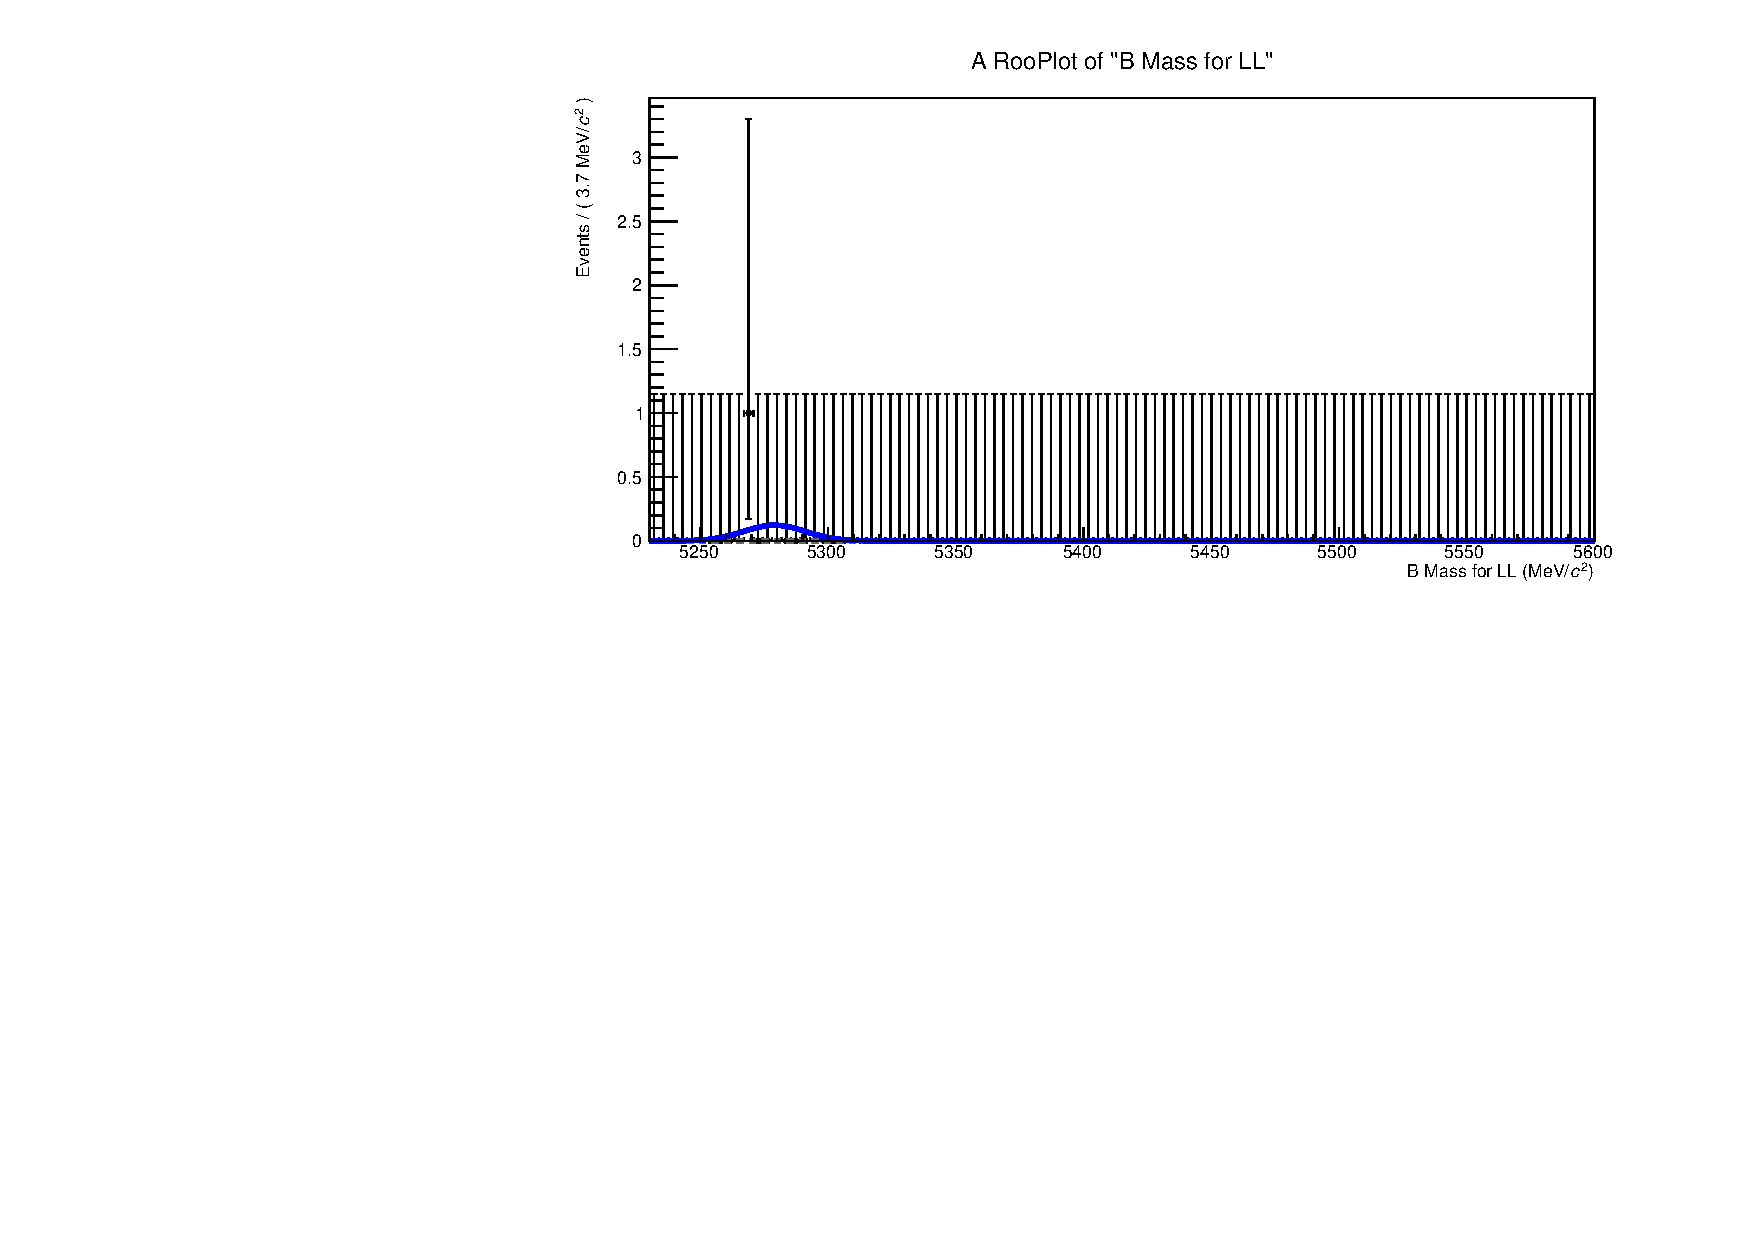
\includegraphics[width=0.7\linewidth]{figures/backgrounds/B2DpipipiFit_KPi_LL_FD5_run2.pdf}
\put(-100,100) {(b)}
\caption{Fits to the Run 2 refitted B mass taking \decay{\Dz}{\Km\pip} candidates from the \KS mass sidebands after requiring the FD significance to be (a) greater than 0 and (b) greater than 5$\sigma$.}
\label{strangelessfits}
\end{figure}

\subsubsection{Non-resonant \boldmath$B \to DK_s\pi$}
\label{sec:backgrounds:non-resonant}

The \Kstarm meson has a large natural width (about 50\mevcc~\cite{PDG2016}) therefore \decay{\Bm}{\D\KS\pim} may be non-negligible in this region, which would affect the measurement of \Pgamma. The purity of the \Kstarm in the sample can be increased by, firstly by only accepting \Kstarm candidates that have a reconstructed mass within 75\mevcc of the known mass and secondly by exploiting the vector properties of the signal decay. 

As the \Kstarm meson is a vector meson, the \decay{\Bm}{\D\Kstarm} decay is a Scalar $\to$ Scalar Vector decay, forcing the \Kstarm to be longitudinally polarised due to the conservation of angular momentum. This structure of the decay can be observed using the \KS helicity angle, $\theta_{\KS}$, which is defined as the angle between the \KS and the \Bm meson pion in the \Kstarm rest frame, as illustrated in Figure \ref{helicityangle}. This angle, $\cos(\theta_{\KS})$, follows a parabolic distribution for pure \decay{\Bm}{\D\Kstarm}, as shown in Figure \ref{helicitycut}~\footnote{The \KS helicity angle distribution is not symmetric. The asymmetry in this variable, manifest in both data and simulation, is due to the momentum and transverse momentum selections placed on the bachelor pion in the stripping stage of the selection.}. 

\begin{figure}
\centering
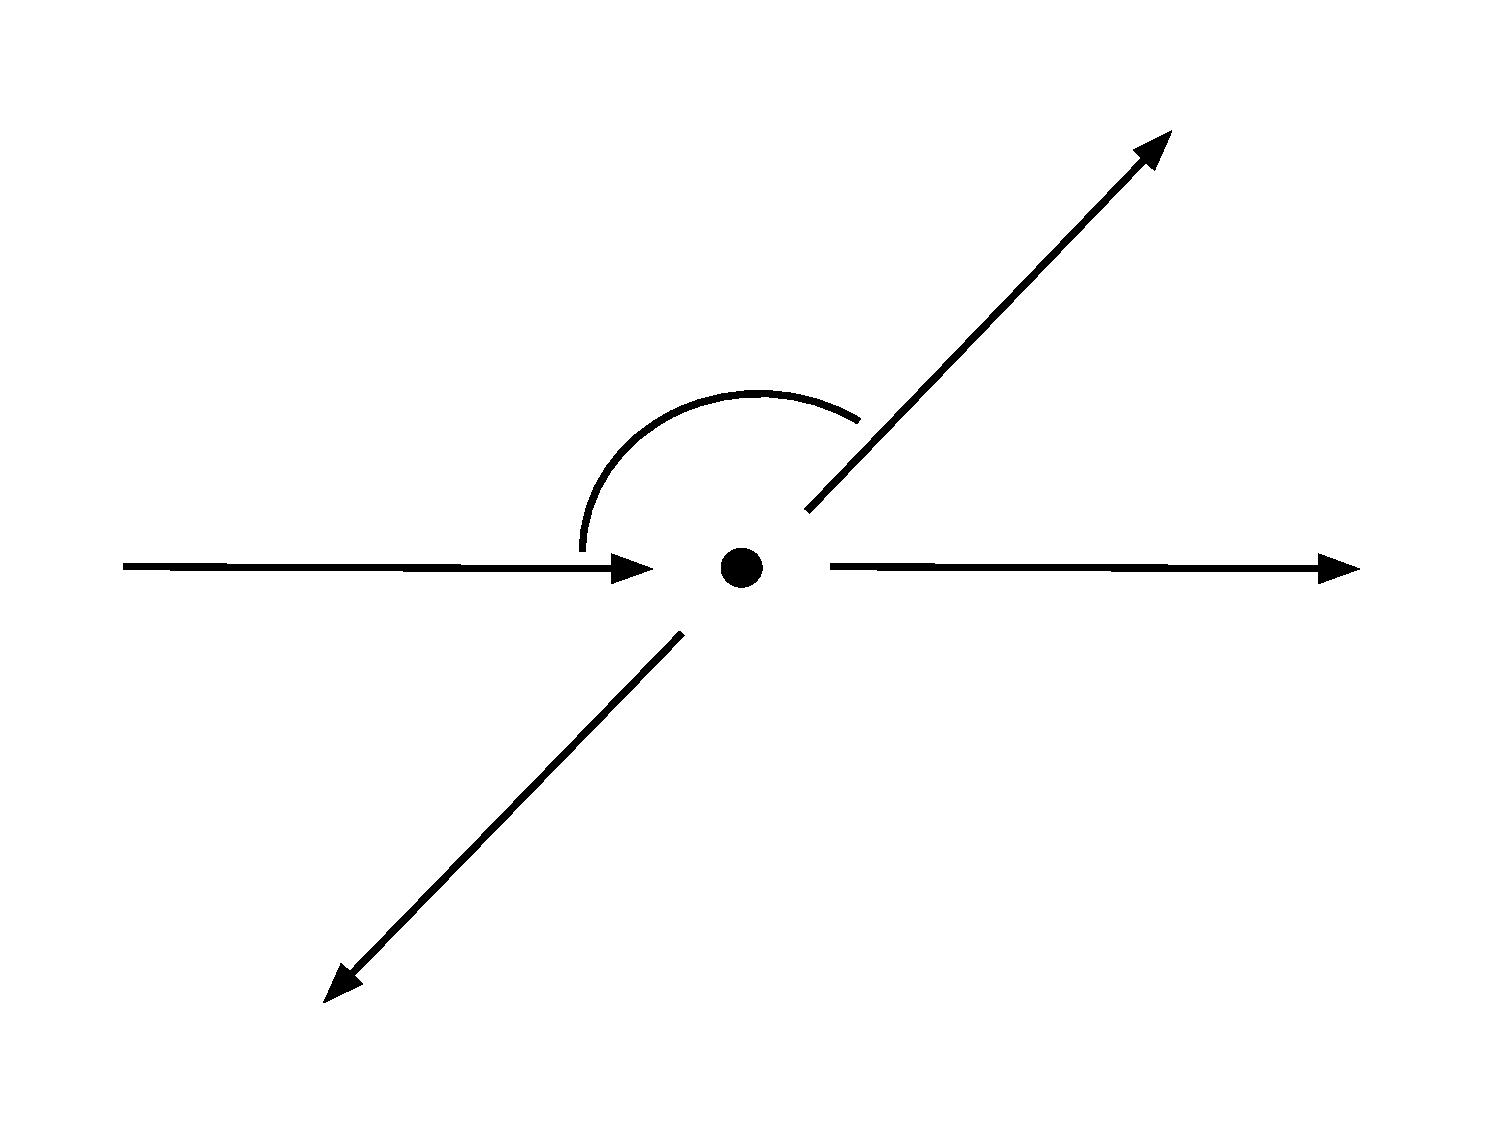
\includegraphics[width=0.5\linewidth]{figures/backgrounds/helicityangle.pdf}
\put(-200,85) {\Bm}
\put(-125,115) {$\theta_{\KS}$}
\put(-30,85) {\Dz}
\put(-75,140) {\KS}
\put(-165,40) {\pim}
\put(-100,60) {\Kstarm}
\caption{Diagram of particles in the \Kstarm rest frame, illustrating the definition of the \KS helicity angle, $\theta_{\KS}$.}
\label{helicityangle}
\end{figure}

\begin{figure}[h]
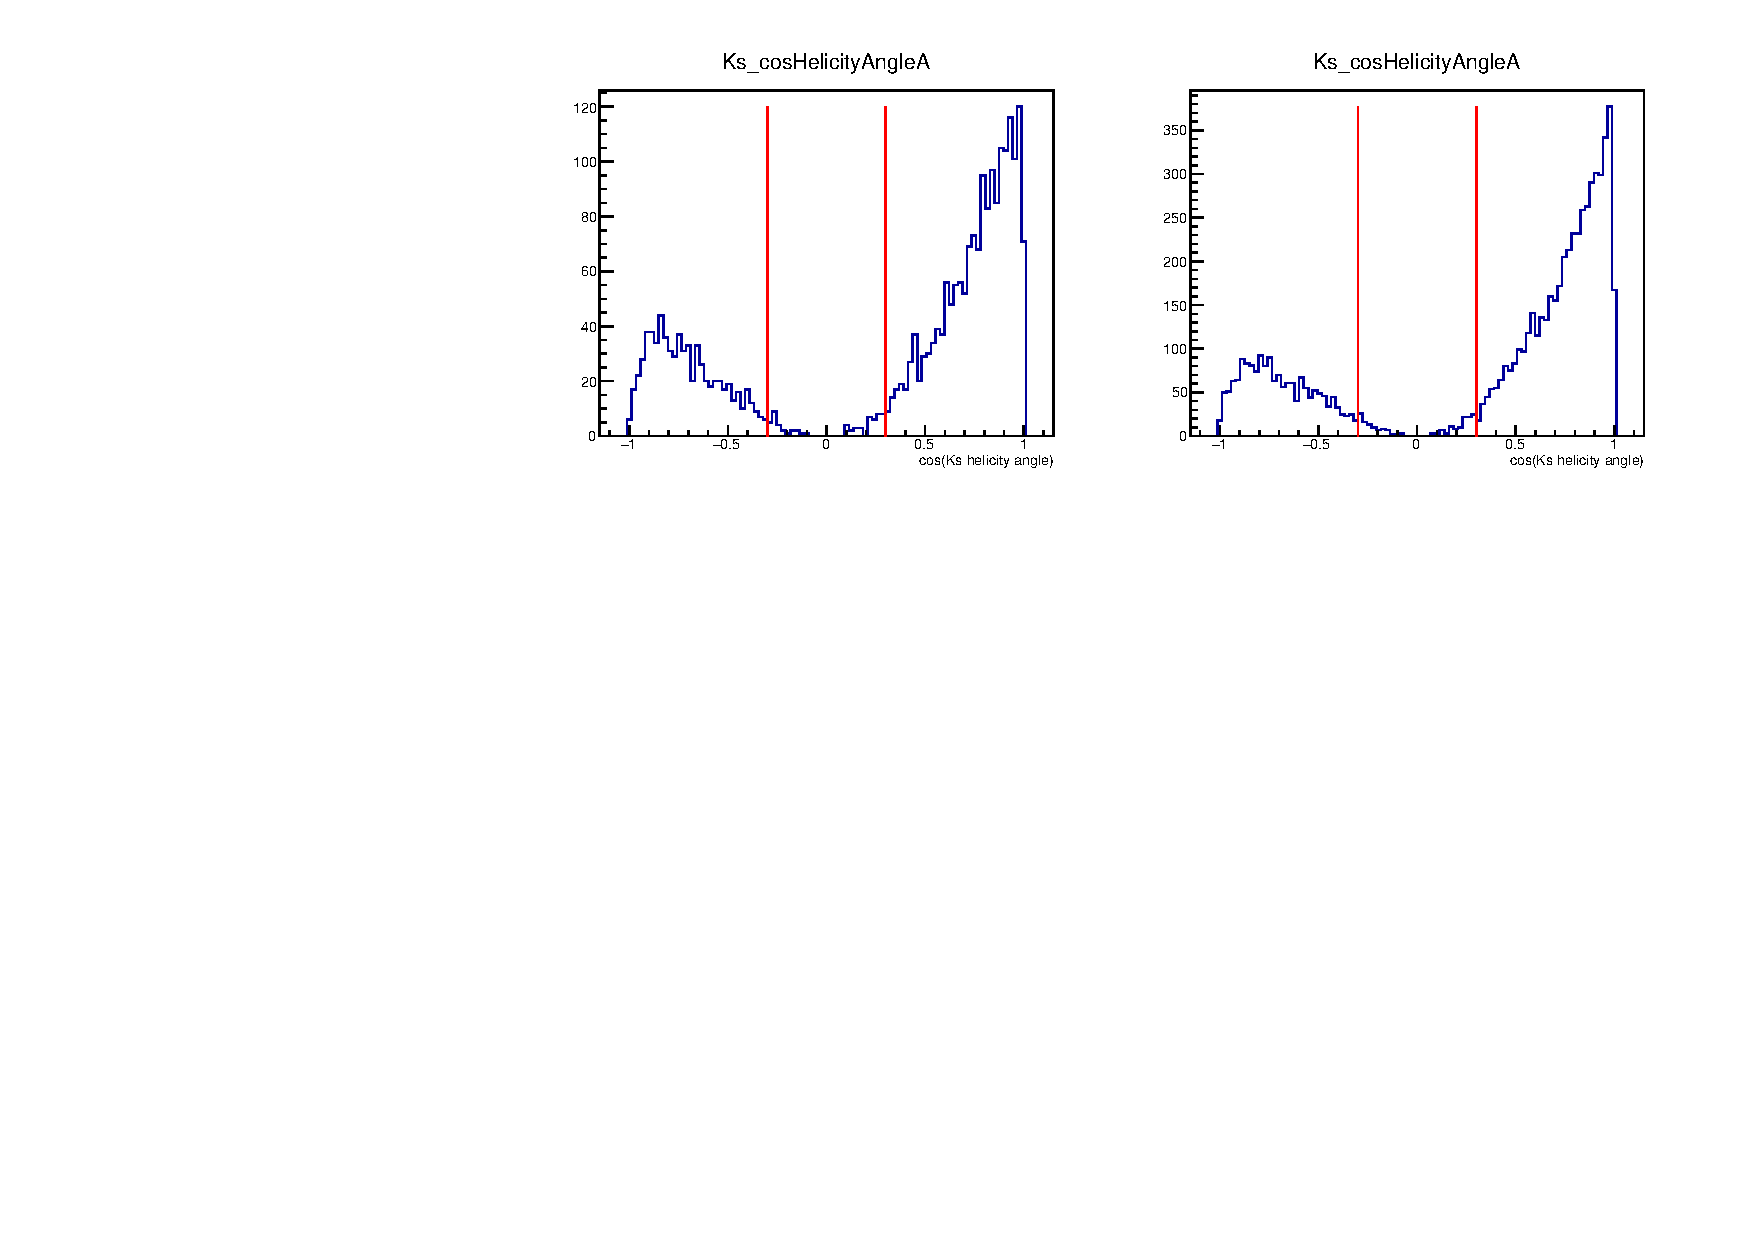
\includegraphics[width=\linewidth]{figures/backgrounds/KsHelicityCut.pdf}
\put(-380,100) {(a)}
\put(-170,100) {(b)}
\caption{Distribution of $\cos(\theta_{\KS})$ from a simulated sample of \kpi events for (a) LL candidates and (b) DD candidates. The red lines represent the region $\cos(\theta_{\KS})$ that is rejected in the selection.}
\label{helicitycut}
\end{figure}

By removing candidates that have a small absolute value of $\cos(\theta_{\KS})$ a large amount of non-resonant \decay{\Bm}{\D\KS\pim} and combinatorial background can be removed while retaining almost all of the pure \decay{\Bm}{\D\Kstarm} signa. The combinatoric background is roughly uniform in $\cos(\theta_{\KS})$, as shown in Figure \ref{Kshelicitybkg}. Removing events with an absolute value of $\cos(\theta_{\KS})$ less than 0.3 retains 97\% of true \decay{\Bm}{\D\Kstarm} decays, while rejecting 30\% of the combinatoric background. The optimisation of the \Kstarm mass and \KS helicity angle selection is discussed in detail in Section \ref{sec:cpfit:optimisation}.

\begin{figure}
\centering
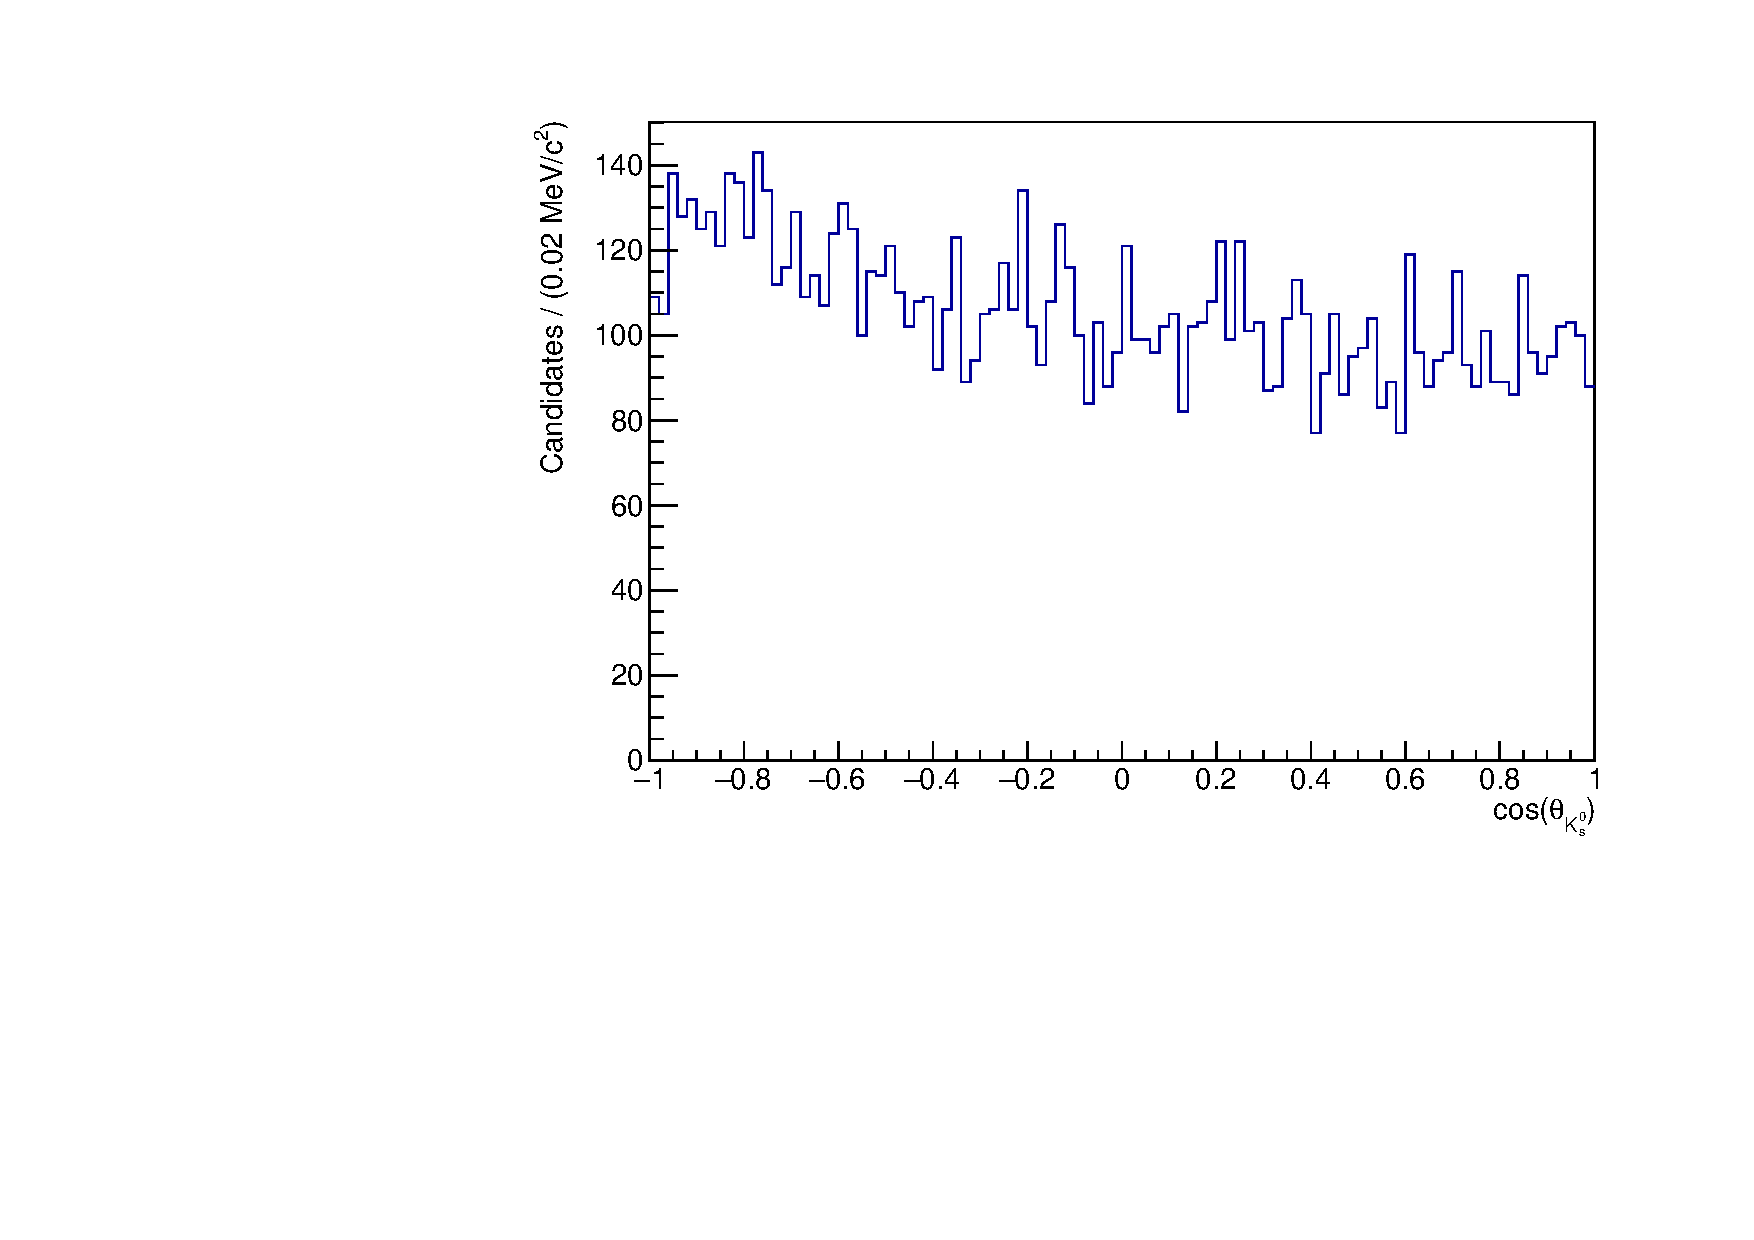
\includegraphics[width=0.5\linewidth]{figures/backgrounds/Kshelicity_background.pdf}
\caption{Distribution of the cosine of \KS helicity angle in \kpi combinatoric background.}
\label{Kshelicitybkg}
\end{figure}

\subsubsection{Crossfeed background}
\label{sec:backgrounds:crossfeed}

As discussed in Section \ref{sec:selection:pid}, the \Bm mass spectrum for the doubly Cabibo suppressed ADS mode, \pik, can contain background events coming from the favoured \kpi mode, where the \Dz daughter mass hypotheses are swapped, i.e. the kaon is misidentified as a pion and the pion is misidentified as a kaon. When considering the two-body \Dz decay modes, the favoured \kpi mode has a branching ratio 281 times higher than the \pik mode~\cite{PDG2016}. Particle identification requirements, detailed in Section \ref{sec:selection:pid}, on the \Dz daughters significantly reduce this background, however in order to bring it down to negligible levels a veto must be applied. An alternative \Dz mass, $m(D_{\text{swapped}})$, is calculated where the \Dz meson is reconstructed with both daughter mass hypotheses are swapped. The veto applied requires $m(D_{\text{swapped}})$ to be greater than 15 MeV away from the known \Dz mass. This veto is illustrated in Figure \ref{Dmassveto}, which shows the distributions from simulated samples for DD candidates in Run 1. Figure \ref{Dmassveto} (a) is the \Dz mass distribution with the correct daughter mass hypothesis, therefore this is what the $m(D_{\text{swapped}})$ distribution would look like for the doubly misidentified background. Similarly, Figure \ref{Dmassveto} (b) is the \Dz mass distribution with the swapped daughter mass hypothesis, therefore this is what the $m(D_{\text{swapped}})$ distribution would look like for the signal. The veto is only applied to the \pik mode in this analysis. It removes 91.2\% of doubly misidentificated background, corresponding to events that lie within the red lines in Figure \ref{Dmassveto} (a), while maintaining a 92.5\% signal efficiency, corresponding to events that lie outside the red lines in Figure \ref{Dmassveto} (b).

\begin{figure}[h]
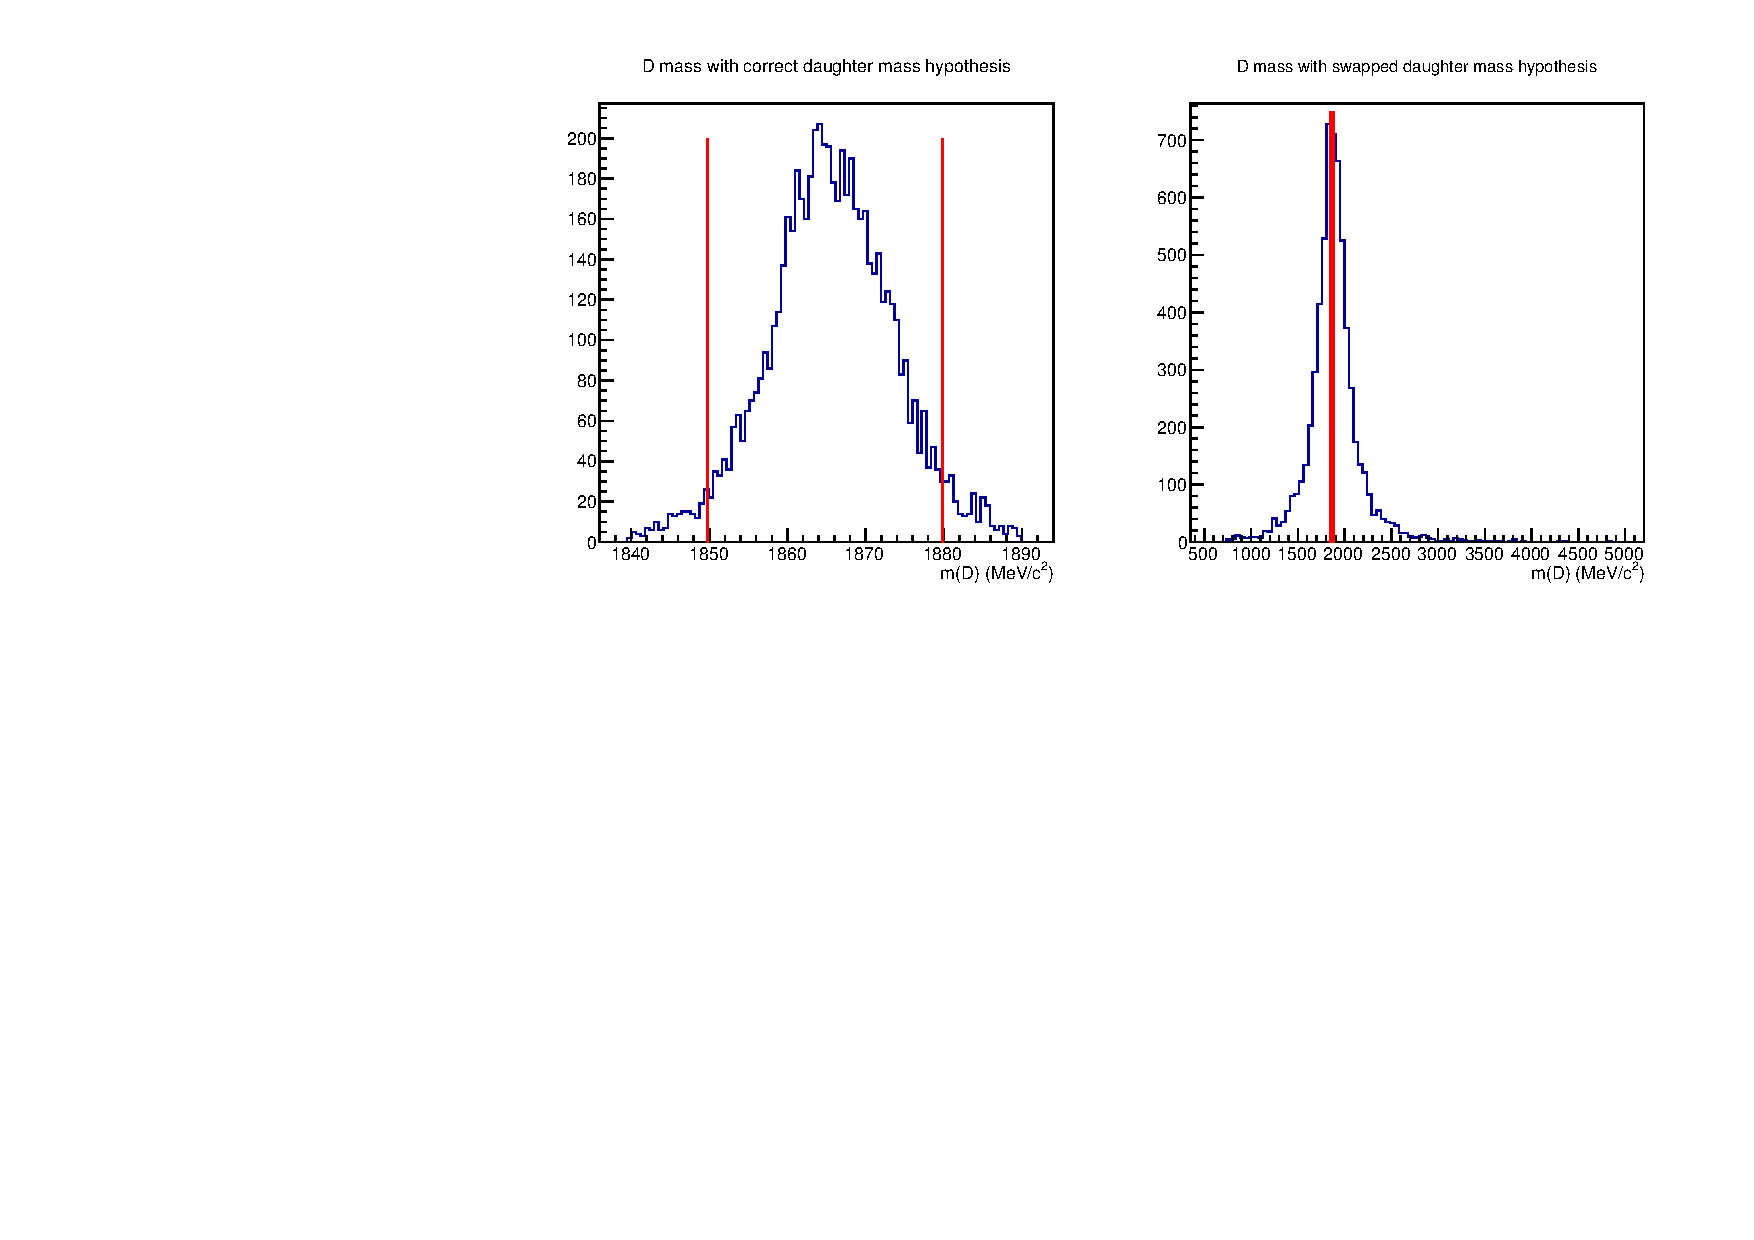
\includegraphics[width=\linewidth]{figures/backgrounds/Dmassveto.pdf}
\put(-380,150) {(a)}
\put(-170,150) {(b)}
\caption{Distributions from simulated samples for DD candidates in Run 1 showing \Dz mass with (a) the correct \Dz daughter mass hypothesis and (b) the swapped \Dz daughter mass hypothesis. Events within the red lines correspond to those removed by the double misidentification veto applied to the \pik mode.}
\label{Dmassveto}
\end{figure}

For the four-body modes, the equivalent background can appear in the suppressed \pikpipi mode due to contamination from the favoured \kpipipi. In this case, there are two \pip mesons that could be misidentified as a \Kp meson, therefore two vetos are be applied. The two possible alternative \Dz masses are reconstructed as a swapped mass hypothesis, one where the kaon is swapped with the lower momentum pion, $m(D_{\text{swapped}}^{\text{low p}})$, and the other where the kaon is swapped with the higher momentum pion, $m(D_{\text{swapped}}^{\text{high p}})$. The veto is applied to both these reconstructed masses as shown in Figure \ref{Dmassveto4body}.

\begin{figure}[h]
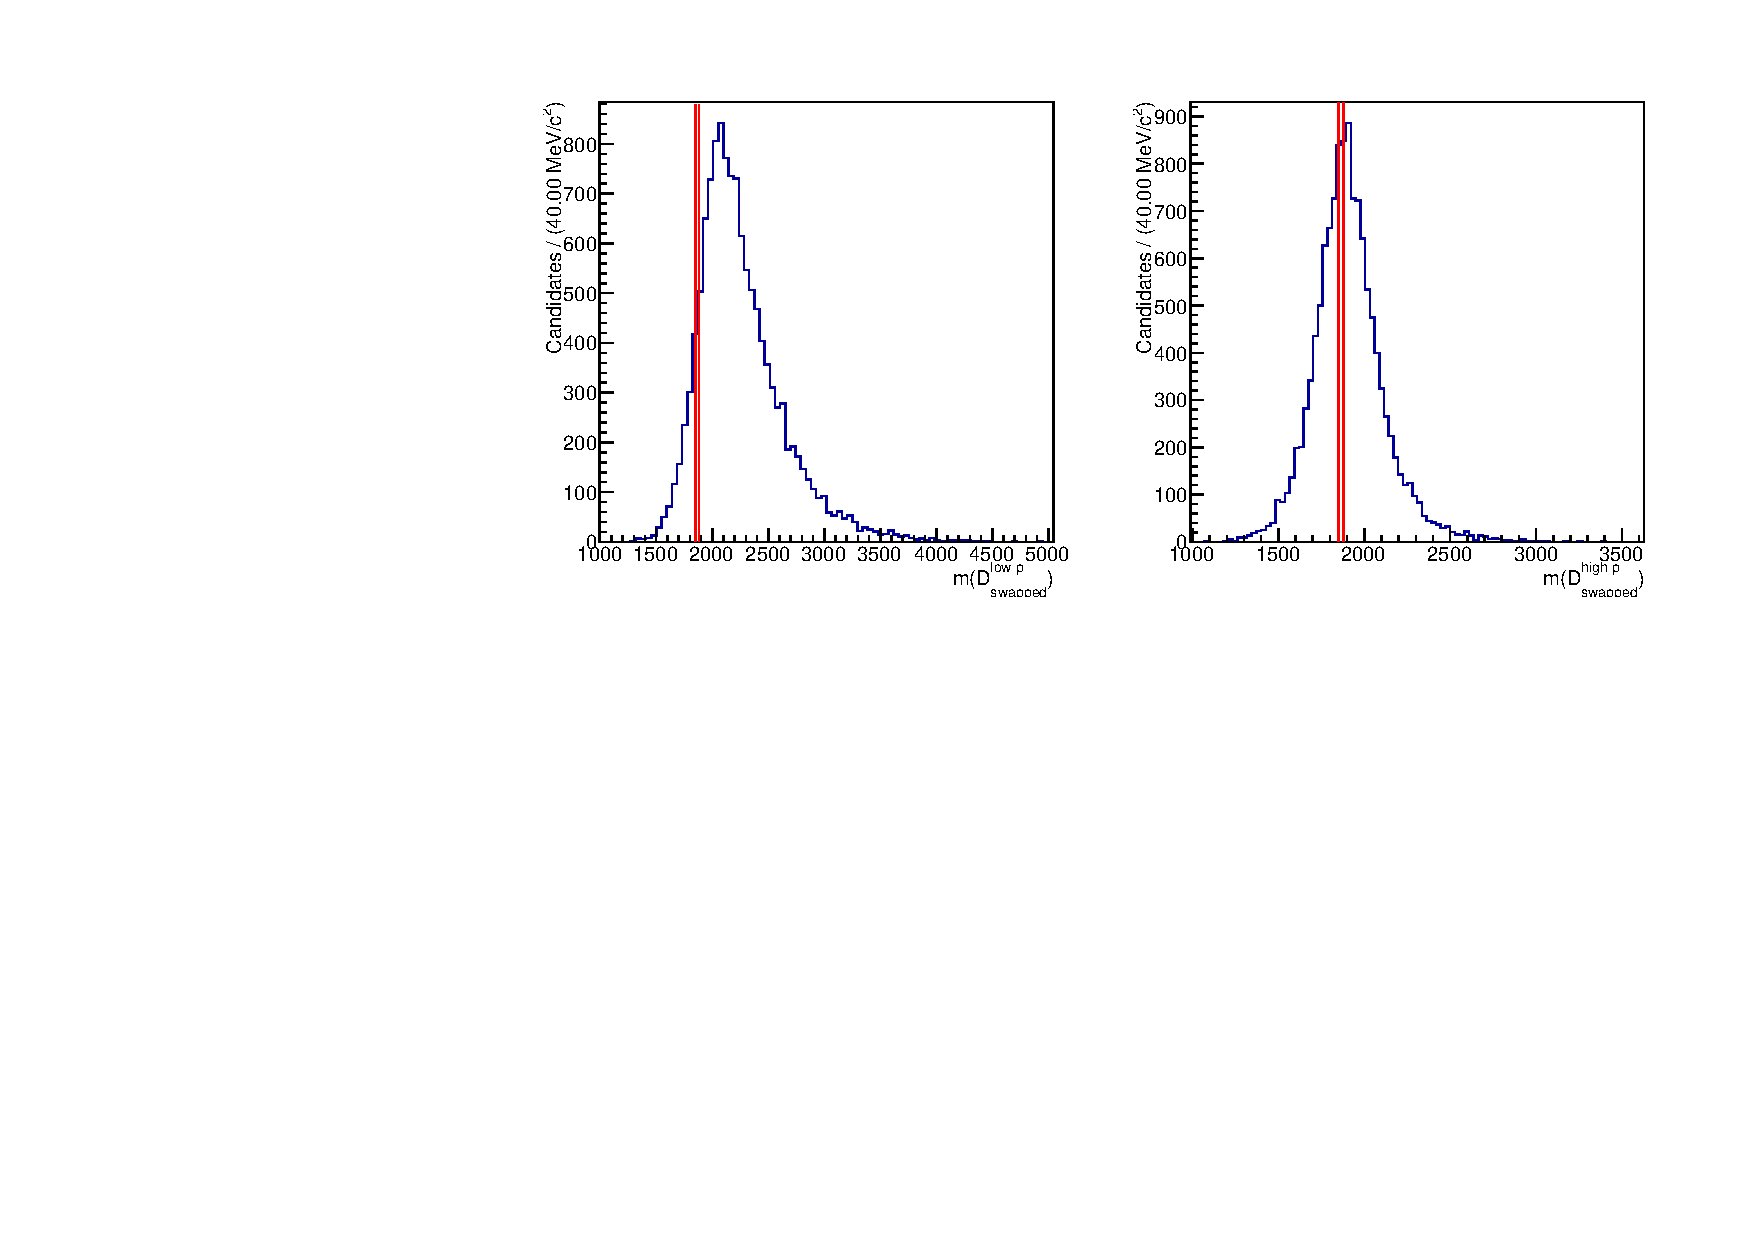
\includegraphics[width=\linewidth]{figures/backgrounds/Dmassveto_4body.pdf}
\put(-380,150) {(a)}
\put(-170,150) {(b)}
\caption{Distributions from simulated samples for DD candidates in Run 2 showing the swapped \Dz daughter mass hypothesis where (a) the kaon is swapped with the lower momentum pion and (b) the kaon is swapped with the higher momentum pion. The red lines correspond to the double misID veto selection window applied to the suppressed mode.}
\label{Dmassveto4body}
\end{figure}

In addition to the double misidentification veto, the selection requirement on the reconstructed \Dz mass and the PID requirements, discussed in Sections \ref{sec:selection:strippingandtrigger} and \ref{sec:selection:pid}, both help to reduce this crossfeed background. In order to determine the overall crossfeed contamination in the suppressed \pik mode the efficiency of the \Dz mass window, double misidentification veto and PID requirements are taken into account for both the normal and swapped \Dz mass hypothesis. Tables \ref{crossfeedtwobody} and \ref{crossfeedfourbody} show the expected proportion of crossfeed events in both the two- and four-body ADS modes, relative to the signal. These results show that this crossfeed background is negligible at less than 0.1\% of the signal.

\begin{table}
\centering
\begin{tabular}{c|cc}
& \runone & \runtwo \\
\hline
LL & $9.5 \times 10^{-3}$ & $5.6 \times 10^{-3}$ \\
DD & $6.5 \times 10^{-3}$ & $5.3 \times 10^{-3}$ \\
\end{tabular}
\caption{The proportion \kpi events expected in the \Bm mass spectrum of the suppressed \pik mode relative to the total \pik signal yield.}
\label{crossfeedtwobody}
\end{table}

\begin{table}
\centering
\begin{tabular}{c|cc}
& \runone & \runtwo \\
\hline
LL & $2.7 \times 10^{-3}$ & $1.4 \times 10^{-3}$ \\
DD & $1.0 \times 10^{-3}$ & $6.3 \times 10^{-4}$ \\
\end{tabular}
\caption{The proportion \kpipipi events expected in the \Bm mass spectrum of the suppressed \pik mode relative to the total \pikpipi signal yield.}
\label{crossfeedfourbody}
\end{table}


\subsubsection{\boldmath \decay{\Lb}{\Lc\Kstar} background in the \kk mass spectrum}
\label{sec:backgrounds:Lb2LcKst}

An additional source of background in the \kk \Bm mass spectrum comes from the decay \decay{\Lb}{\Lc(p\Km\pip)\Kstarm}, where the proton is misidentified as \Kp and the \pip is missed in the reconstruction. The decay mode \decay{\Lc}{p\Km\pip} accounts for over 6\% of the \Lc branching fraction~\cite{PDG2016}, whereas \Lc decays that may contribute as background to the other \Dz decay modes, e.g. \decay{\Lc}{p\pim\pip}, are suppressed by an order of magnitude. Therefore, this background is only considered for the \kk decay model.

The branching fraction of \decay{\Lb}{\Lc(p\kaon\pi)\Kstarm} is roughly five times larger than the \kk branching fraction. As these decays have similar topologies, the selection efficienies are expected to be similar, with the exception of the requirement on the reconstructed \Dz mass, which significantly reduces this background. Additionally, this background is significantly reduced by the PID requirements on the \Dz daughters, as the background requires the proton to be incorrectly identified as a \Kp meson. Taking these considerations into account, this background is expected to contribute O(1) event to the \kk mass spectrum. The PID requirements on the \Dz daughters cannot be increased, to ensure this background is reduced to negligible levels, due to the effect on the signal efficiency. Therefore, in order to account for this background, it is modelled and included as a component to the fit, discussed in more detail in Section \ref{sec:cpfit:Lb2LcKst}. 

\subsubsection{\boldmath \decay{\Bs}{\Dzb\bar{K}^{*}(1410)^0} background}
\label{sec:backgrounds:bs}

The decay \decay{\Bs}{\Dzb\bar{K}^{*}(1410)^0} or $\Dzb K_1(1400)^0$, \decay{(K_1,K^*)}{K^{*}(892)^-\pip}, where the \pip is missed in reconstruction is considered as a possible background contribution. The branching fraction of this mode is similar to that of the signal and the same particles are present in this background as are in the signal decay, therefore this background could be dangerous. Due to this background having the favoured mode corresponding to the combination of \Dzb and \Kstarm, it is considered as a contribution in the ADS mode. As the reconstruction of this background in the ADS mode requires the \pip meson to be missed, the reconstructed \Bm would fall in a region just below the signal peak. The fit used to extract the \CP observables has a lower mass limit of 5230\mevcc, therefore this background will be almost entirely removed. However, it is possible that a small contribution still remains and contributes to the signal region. 

The \Bs background contribution can be estimated from the branching fraction and the efficiency of this background through the \btodkst selection. The \decay{\Bs}{\Dzb\bar{K}^{*}(1410)^0} branching fraction of $\left(3.9 \pm 3.5\right) \times 10^{-4}$~\cite{PDG2016}. Due to the similar topologies of the signal and background decays, the selection efficiency of the \decay{\Bs}{\Dzb\bar{K}^{*}(1410)^0} is considered the same as for \btodkst, except for the efficiency of the requirement that the \Bm mass must be above 5230\mevcc, given by $\epsilon_{\Bs}(B\ mass\ > 5230\mevcc)$. This assumption allows an estimate for the upper limit of the background contribution, as shown in \eqn\ref{Bscalc}. 

\begin{multline}
N(\decay{\Bs}{\Dzb\bar{K}^{*}(1410)^0}) = N(\btodkst) \times \frac{\BF(\decay{\Bs}{\Dzb\bar{K}^{*}(1410)^0})}{\BF(\btodkst)} \\ \times \frac{\epsilon_{\Bs}(B\ mass\ > 5230\mevcc)}{\epsilon_{\Bm}(B\ mass\ > 5230\mevcc)}
\label{Bscalc}
\end{multline}
In order to calcualte the efficiency, $\epsilon_{\Bs}(B\ mass\ > 5230\mevcc)$, a simulated sample of \decay{\Bs}{\Dzb\bar{K}^{*}(1410)^0}, \decay{\bar{K}^{*}(1410)^0}{K^{*}(892)^-\pip} events is generated, where the \pip is missed in reconstruction. The efficiency of the \Bm mass requirement being greater than 5230\mev is found to be $6.4 \times 10^{-4}$. 

This calculation gives an upper limit estimate of $2.6 \pm 2.6$ \decay{\Bs}{\Dzb\bar{K}^{*}(1410)^0} events in \pik mode above 5230\mev. This estimated \Bs background is used to assign a systematic uncertainty to the \CP observables, discussed in more detail in Section \ref{sec:systematics}.


\subsubsection{Lambda contamination}
\label{sec:backgrounds:contamination}

The \decay{\KS}{\pip\pim} decay could have contamination coming from \decay{\Lz}{\proton\pim}, where the proton is reconstructed as a pion. It is not possible to determine possible \Lz contamination from the \KS invariant mass spectrum, where one of the \KS daughters is assigned the proton mass, because a peak at the \Lz mass cannot be distinguished from the variation near the low mass threshold. In order to distinguish between \KS decays and \Lz contamination the Armenteros-Podolanski (AP) plot is used~\cite{APplot}. The transverse momentum of the daughters with respect to the mother particle, $p_T$, is plotted against the longitudinal momentum asymmetry, which is defined as,

\begin{equation}
\frac{p_L^+ - p_L^-}{p_L^+ + p_L^-}
\label{longitudinalpasy}
\end{equation}

where $p_L^{\pm}$ is the longitudinal momentum of the daughter particles with respect to the direction of the mother. The decay products of the \decay{\KS}{\pip\pim} decay have the same mass and therefore on average their momenta is symmetrically distributed. Whereas for the \decay{\Lz}{\proton\pim}, the proton would, on average, take a larger proportion of the momentum resulting in an asymmetric distribution. Contamination from \Lz baryons would be clearly seen as a distinct structure on the AP plot, as illustrated in Figure \ref{apexample}. 

\begin{figure}
\centering
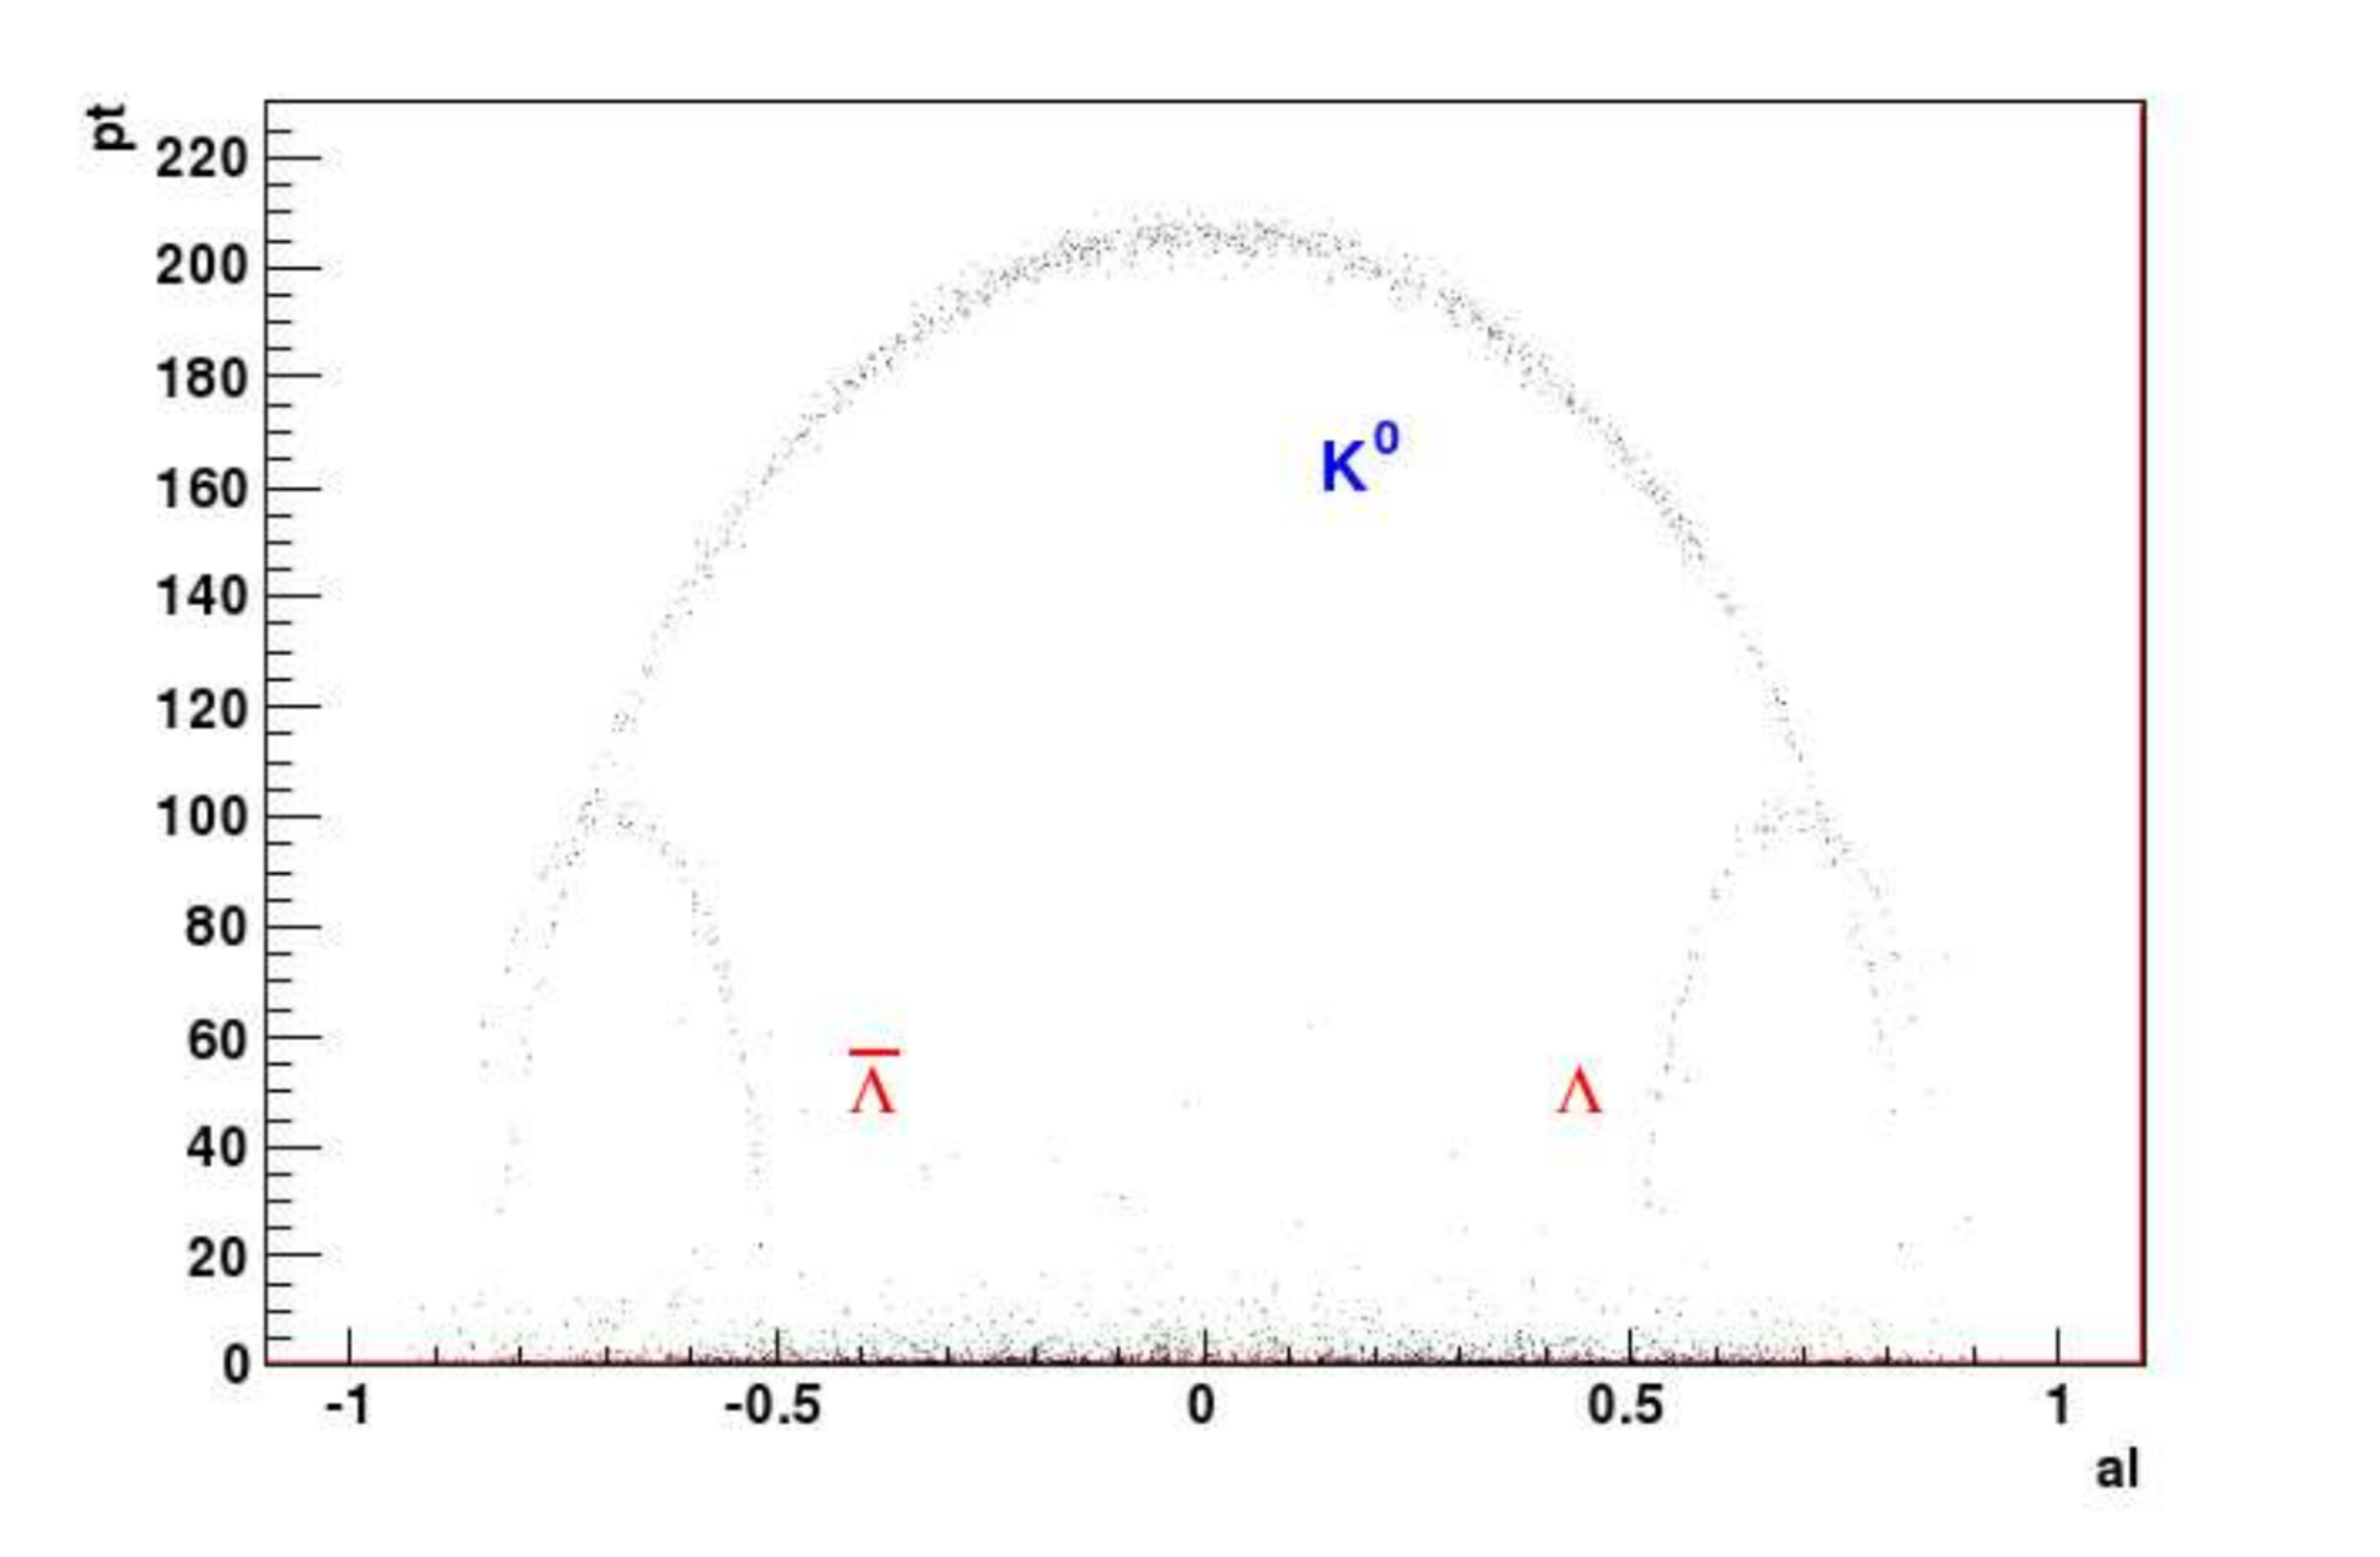
\includegraphics[width=0.5\linewidth]{figures/backgrounds/APfromPaper.pdf}
\caption{An example Armenteros-Podolanski plot showing where the signal regions for \KS, \Lz and \Lbar are located in the AP plane. Reproduced from Ref.~\cite{APplot}.}
\label{apexample}
\end{figure}

The resulting AP plots from this analysis for both data and simulation are shown in Figure \ref{applots}, these curves are the same shape as the expected distribution for a sample of pure \KS mesons. Therefore, there is no contamination from \decay{\Lz}{\proton\pim} decays in the data.

\begin{figure}[h]
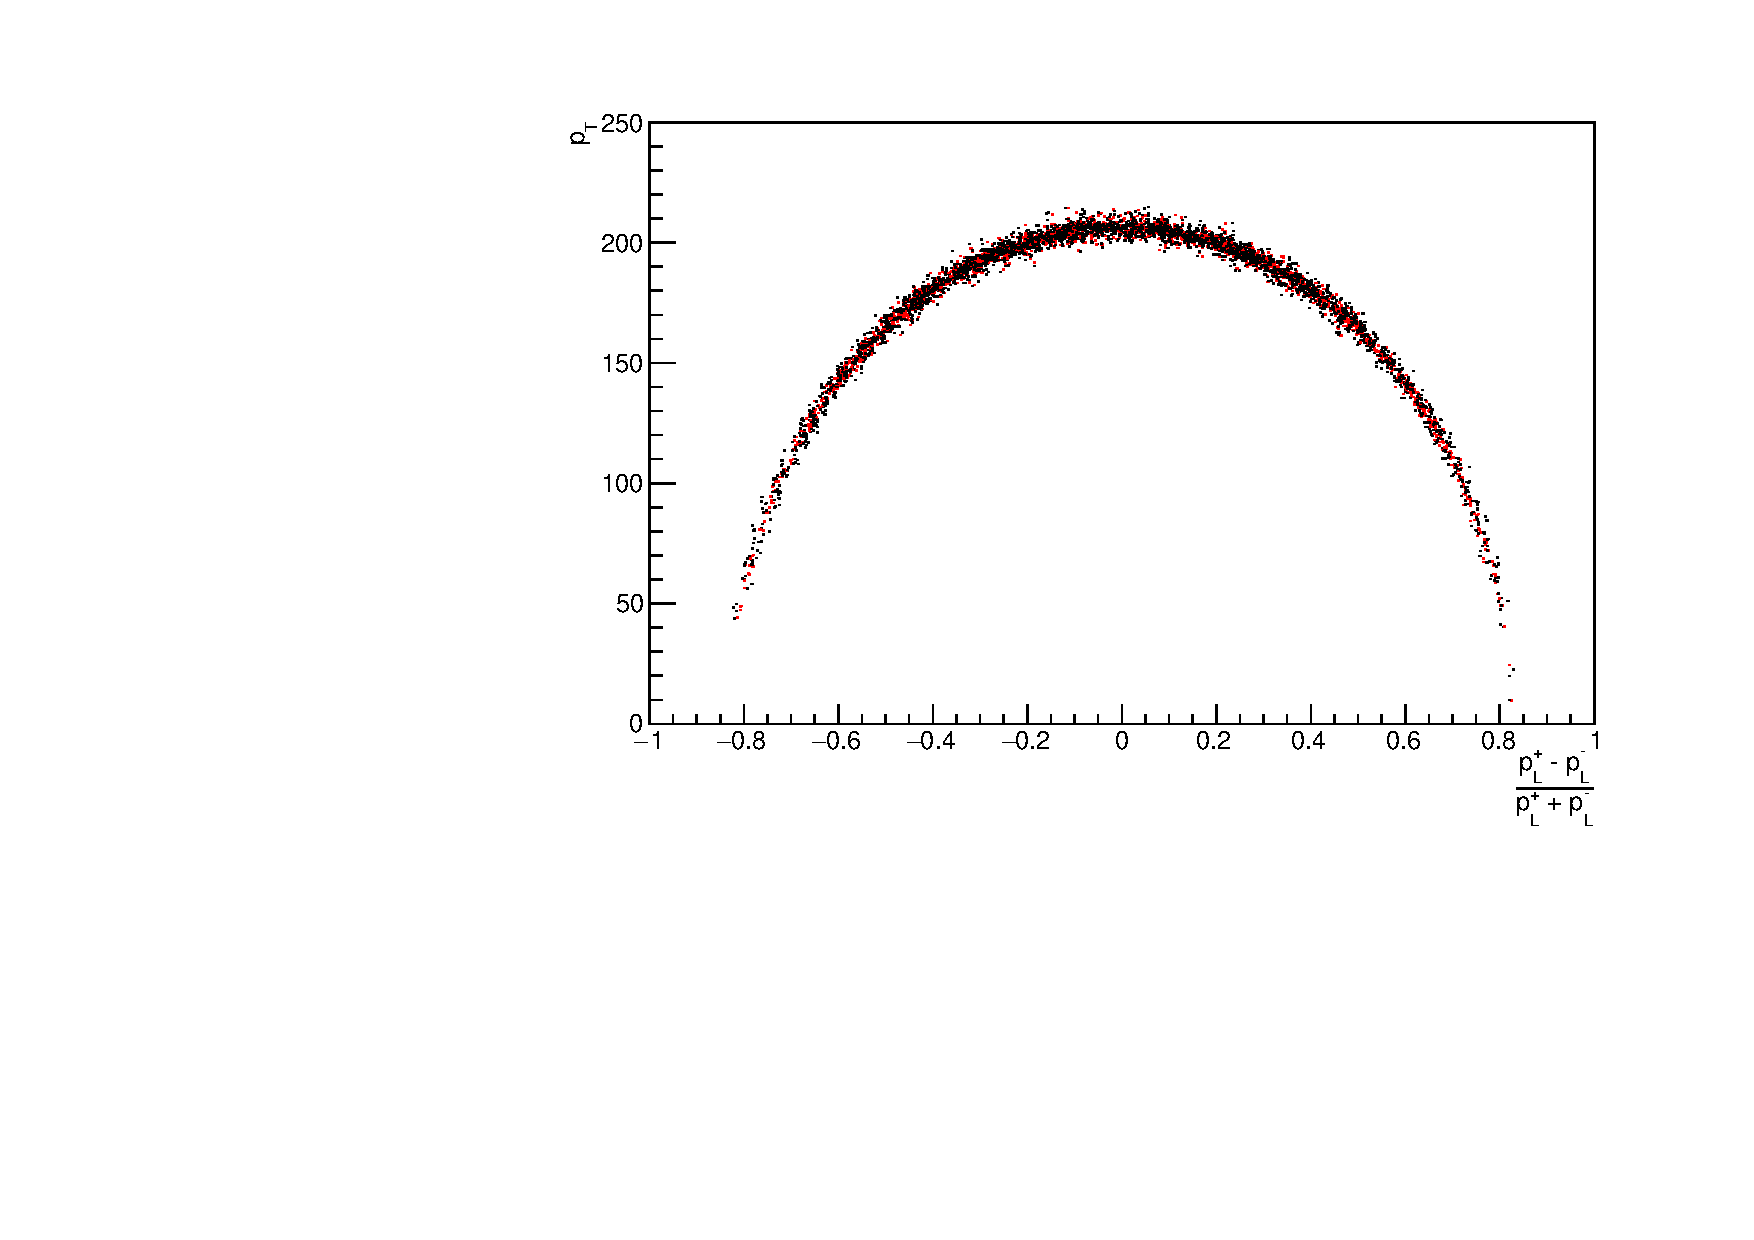
\includegraphics[width=0.5\linewidth]{figures/backgrounds/APplot_LL.pdf}
\put(-180,100) {(a)}
\hfill
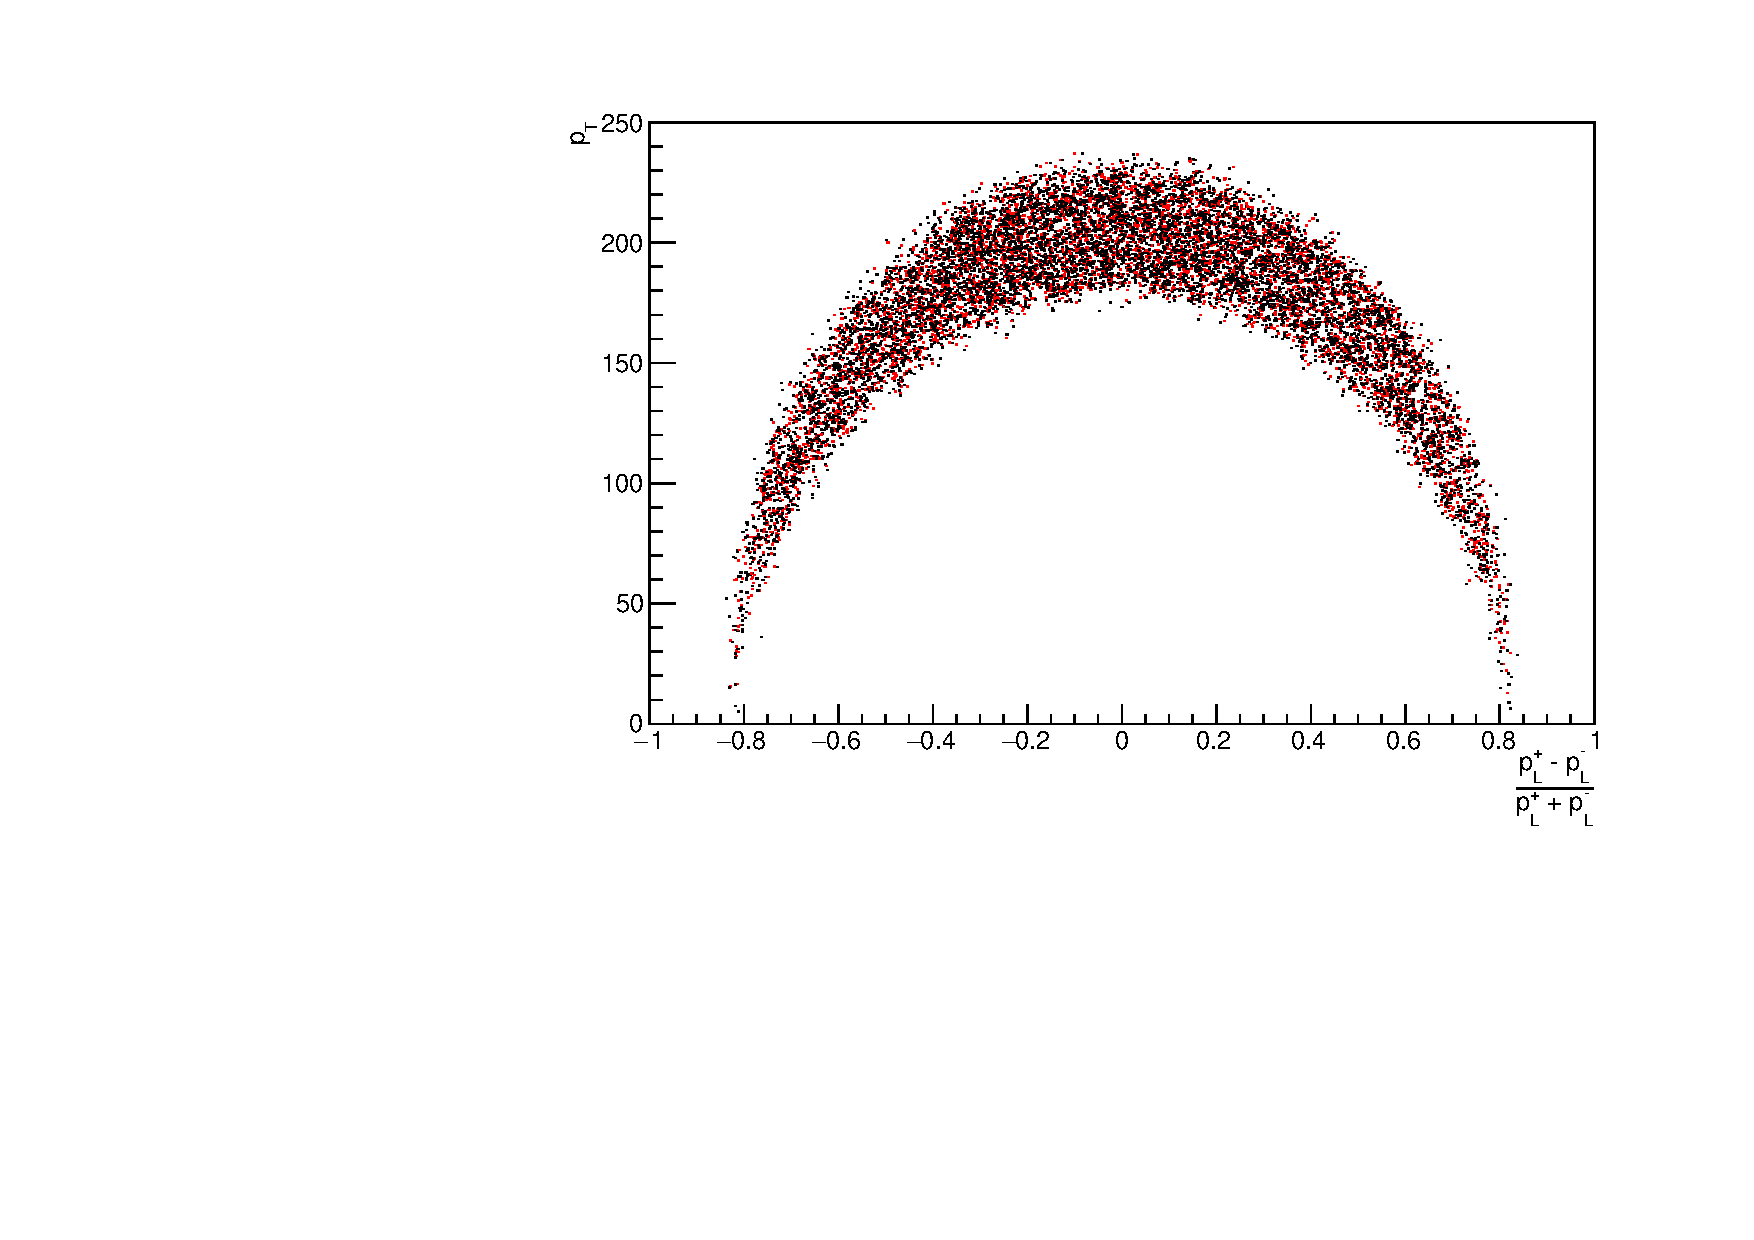
\includegraphics[width=0.5\linewidth]{figures/backgrounds/APplot_DD.pdf}
\put(-180,100) {(b)}
\caption{Armenteros-Podolanski plots for both data (black) and simulation (red) for (a) LL, and (b) DD candidates. The $p_T$ values on the y axis are the transverse momentum of the daughters with respect to the mother particle and the x axis contains the longitudinal momentum asymmetry, defined in Equation \ref{longitudinalpasy}.}
\label{applots}
\end{figure}


\subsubsection{\boldmath \decay{\B}{\D\KS\kaon} background}
\label{sec:backgrounds:b2dkks}

The decay \decay{\Bm}{\D\KS\Km} has a branching fraction of $5.5 \times 10^{-4}$~\cite{PDG2014}, which is similar to the signal \decay{\Bm}{\D\Kstarm(\KS\pim)} branching fraction. However, nearly all of this background is removed by the requirements that the reconstructed \Kstarm mass must be within 75 \mevcc of the known \Kstar mass and the DLLK of the bachelor pion must be less than four. This PID requirement on the bachelor pion reduces the rate of misidentification of the bachelor pion, i.e. the efficiency of a \Km passing the bachelor PID requirement, which suppresses the background by about 8\%. The efficiency of the \Kstarm mass selection when applied to the simulated \decay{\Bm}{\D\KS\Km} samples is 3\% for both LL and DD. After accounting for the misidentification rate and selection efficiencies, the expected contribution of \decay{\Bm}{\D\KS\Km} background in the \kpi mass spectrum is less than 1\% of the signal, therefore the decay is considered negligible. Any residual amount is investigated alongside the systematics for the residual low mass background in this region.

\subsection{Multivariate analysis with a Boosted Decision Tree}
\label{sec:selection:bdt}

Various selection requirements are placed on individual variables relating to particles in the decay chain in order to reduce specific background contributions. However, in order to achieve a much lower combinatorial background, while retaining signal events, requires more sophisticated classification techniques. As many variables are correlated with each other, the ability to separate signal from combinatoric background can be improved by using a multivariate analysis (MVA) method, which exploits these correlations between the variables. The MVA implemented in this analysis is a Boosted Decision Tree (BDT)~\cite{Breiman}. Decision trees take a given set of variables from signal and background training samples and construct an algorithm to decide whether a given event corresponds to signal or background. Firstly, the best variable and value is found to split events into two subsets in order to separate signal and background, the process is then repeated for each of the two subsets. This is continuously repeated in order to build a tree, where the nodes at the end are called leaves. If more than half of the weight of a leaf corresponds to signal, it is a signal leaf, where each event is given a value of +1, otherwise it is a background leaf, where each event is given a value of -1. Signal events on a background leaf and background events on a signal leaf are misclassified. In order to stabilise this process many trees are built to construct a weighted average over all the trees. After each tree is built, the misclassified events are reweighted (boosted) and a new tree is build with the rewighted events. The boosting makes misclassified events more likely to be correctly classified in future trees; a particular type of boosting, called gradient boost, is used in this analysis. The result of the process assigns each event a weight from -1 (most background-like) to +1 (most signal-like). 

\subsubsection{Training samples}

A Boosted Decision Tree (BDT) with the gradient boost (BDTG) method using the Toolkit for Multivariate Analysis (TMVA) framework~\cite{TMVA} is employed in order to reduce the combinatorial background level. A separate BDT is trained for LL and DD candidates, named BDTG\_LL and BDTG\_DD respectively. The BDTs are mainly based on topological variables, so are insensitive as to whether the \Dz daughters are kaons or pions. Therefore, the same BDT is used for all of the two-body \Dz decay modes, trained using \kpi decays, and another BDT is used for all of the four-body \Dz decay modes, trained using \kpipipi decays. 

For the two body modes, simulated samples for the decay \kpi were used to provide a signal sample. Events from data in the favoured \kpi mode in the region of \Bm mass above 5600 MeV were used as a sample of background combinatorial events. Generation of simulated events is computationally expensive. A small simulated sample is produced from full \lhcb simulation in order to determine efficiencies. The sample is small due to many generated events failing the reconstruction, however, BDT training requires a significantly larger sample. The available resources are insufficient to simply generate more events. A workaround is employed to remove events at generator level, which are less likely to pass the selection. This reduces the number of events required to be simulated in the \lhcb detector, which is the most computationally expensive part of the reconstruction process. Events are removed on the basis of low momentum or transverse momentum of signal tracks or intermediate particles. The advantage of this approach is that 89\% of generated events are removed, significantly reducing the resource requirement. However, the disadvantage is that the selection has to be more stringent than the final selection and 20\% of events that would have passed are removed. Therefore, the BDT may not be as optimal as it may have been with unlimited resources. This trade-off is deemed acceptable.

For \kpipipi, signal samples of simulated events for the decay \kpipipi, without any selection requirements at generator level, were used. This was possible due to an artefact of the time that each stage of the analysis was performed; at this later time the resource availability improved. Events from data in the favoured \kpipipi mode in the region of \Bm mass above 5600 MeV were used as a sample of background combinatorial events. All samples used in training the BDTs are split into a training and testing sample before being used as an input to the multivariate algorithm.

\subsubsection{Setup and implementation of the multivariate algorithm}

Initial selection requirements are applied to both the signal and background training samples to remove candidates that would not pass the final selection. This allows a more accurate discrimination between signal and background in data. The selection criteria on the training samples are:

\begin{itemize}
\item The \chisq of the decay chain refit per degree of freedom, $\chisq_\text{refit}$, with {\tt D0const}, {\tt KS0const} and {\tt PVconst} constraints, must lie between 0 and 100
\item The \chisqip of the \Bm candidate, with respect to the \Bm vertex, must lie between 0 and 25
\item The reconstructed \Kstarm mass must lie within 500\mevcc of the known \Kstarm mass
\item The reconstructed \KS mass must lie with 15\mevcc of the known \KS mass for LL candidates and 20\mevcc for DD candidates
\end{itemize}
These selection requirements are looser than those applied to the full selection, discussed in Section \ref{sec:selection:strippingandtrigger}. For example, here no requirement is imposed on the reconstructed \Dz mass and the \Kstarm requirement is as wide as 500\mevcc rather than the 75\mevcc used in the full selection. This is because the training samples required for the BDT must be large enough for the multivariate algorithm to distinguish between important differences in the signal and background samples rather than statistical fluctuations in the distributions. Imposing tighter selection is found to reduce the size of the samples to a point where the BDTs would be suboptimal.

Various input variables are used to exploit the topology of the decay; of particular importance are the \chisq per degree of freedom of the decay chain refit, with constraints, $\chisq_\text{refit}$, and the $p_T$ asymmetry between the \Bm candidate and other tracks from the same PV, defined as
\begin{equation}
A_{p_T} = \frac{p_T^B - p_T^{\text{cone}}}{p_T^B + p_T^{\text{cone}}}
\label{ptasy}
\end{equation}
where $p_T^B$ is the $p_T$ of the reconstructed \Bm signal candidate and $p_T^{\text{cone}}$ is the sum of the $p_T$ of all other tracks in a cone of radius 1.50 surrounding the \Bm candidate. This is a quantitative measure of the isolation of the \Bm candidate. Some of the variables are transformed using a logarithm function to increase their separation power. Other input variables used include the logarithm of the \chisqip for the \Bm, bachelor, \Dz and all the \Dz decay products, the logarithm of the \chisqip for the \KS and both its decay products (for LL only) and the $p_T$ of the \KS candidate (for DD candidates only). The variables used in the BDT are slightly different for LL and DD candidates, as the separation power of the \KS variables significantly differs between LL and DD candidates. 

Tables \ref{BDTinputvariables2body} and \ref{BDTinputvariables4body} show the list of input variables, in the two and four-body BDTs respectively, ranked by separation power. The distributions of the two-body BDT input variables in the training signal and background samples are shown in Figures \ref{BDTinputdist2bodyLL} and \ref{BDTinputdist2bodyDD}. The equivalent distributions of the input variables for the four-body BDT are similar. Other variables and other setup of test and training samples were investigated but found to have negligible improvement.

\begin{table}
\centering
\subfloat[Input variables for the two-body BDTs.][Input variables for the two-body BDTs.]{
\begin{tabular}{lll}
Rank & Variable in BDT\_LL & Variable in BDT\_DD \\
\hline
1 & log($\chisq_\text{refit}$) & log($\chisq_\text{refit}$) \\
2 & log(\KS \chisqip) & log(\D daughter kaon \chisqip) \\
3 & log(max \KS daughter \chisqip) & log(Bachelor \chisqip) \\
4 & \B ptasy 1.50 & \B ptasy 1.50 \\
5 & log(\D daug kaon \chisqip) & log(\D daughter pion \chisqip) \\
6 & log(Bachelor \chisqip) & log(\D \chisqip) \\
7 & log(\D \chisqip) & log(\B \chisqip) \\
8 & log(min \KS daughter \chisqip) & \KS $p_T$ \\
9 & log(\D daug pion \chisqip) & - \\
10 & log(\B \chisqip) & - \\
\end{tabular}
\label{BDTinputvariables2body}}
%\caption{Ranking for variables for BDTG\_LL and BDTG\_DD for the two-body BDTs.}
%\label{BDTinputvariables2body}
\qquad
\subfloat[Input variables for the four-body BDTs.][Input variables for the four-body BDTs.]{
\begin{tabular}{lll}
Rank & Variable in BDT\_LL & Variable in BDT\_DD \\
\hline
1 & log($\chisq_\text{refit}$) & log($\chisq_\text{refit}$) \\
2 & log(\KS \chisqip) & $A_{\pt}$ \\
3 & $A_{\pt}$ & log(\B \chisqip) \\
4 & log(\B \chisqip) & log(Bachelor \chisqip) \\
5 & log(\D \chisqip) & \KS $p_T$ \\
6 & log(\D daughter kaon \chisqip) & log(\D \chisqip) \\
7 & log(Bachelor \chisqip) & log(max \D daughter \chisqip) \\
8 & log(min \D daughter \chisqip) & log(\D daughter ss \chisqip) \\
9 & log(max \KS daughter \chisqip) & log(\D daughter kaon \chisqip) \\
10 & log(\D daughter ss \chisqip) & log(min \D daughter \chisqip) \\
11 & log(min \KS daughter \chisqip) & - \\
12 & log(max \D daughter \chisqip) & - \\
\end{tabular}
\label{BDTinputvariables4body}}
%\caption{Ranking for variables for BDTG\_LL and BDTG\_DD for the four-body BDTs. The particle name "D daughter ss'' refers to the pion from the \D which has the same sign of the kaon.}
%\label{BDTinputvariables4body}
\caption{List of input variables for the (a) two-body, and (b) four-body, BDTs, ranked by separation power. For the four-body BDTs, the particle name "D daughter ss'' refers to the pion from the \D which has the same sign of the kaon.}
\end{table}

\begin{figure}
\centering
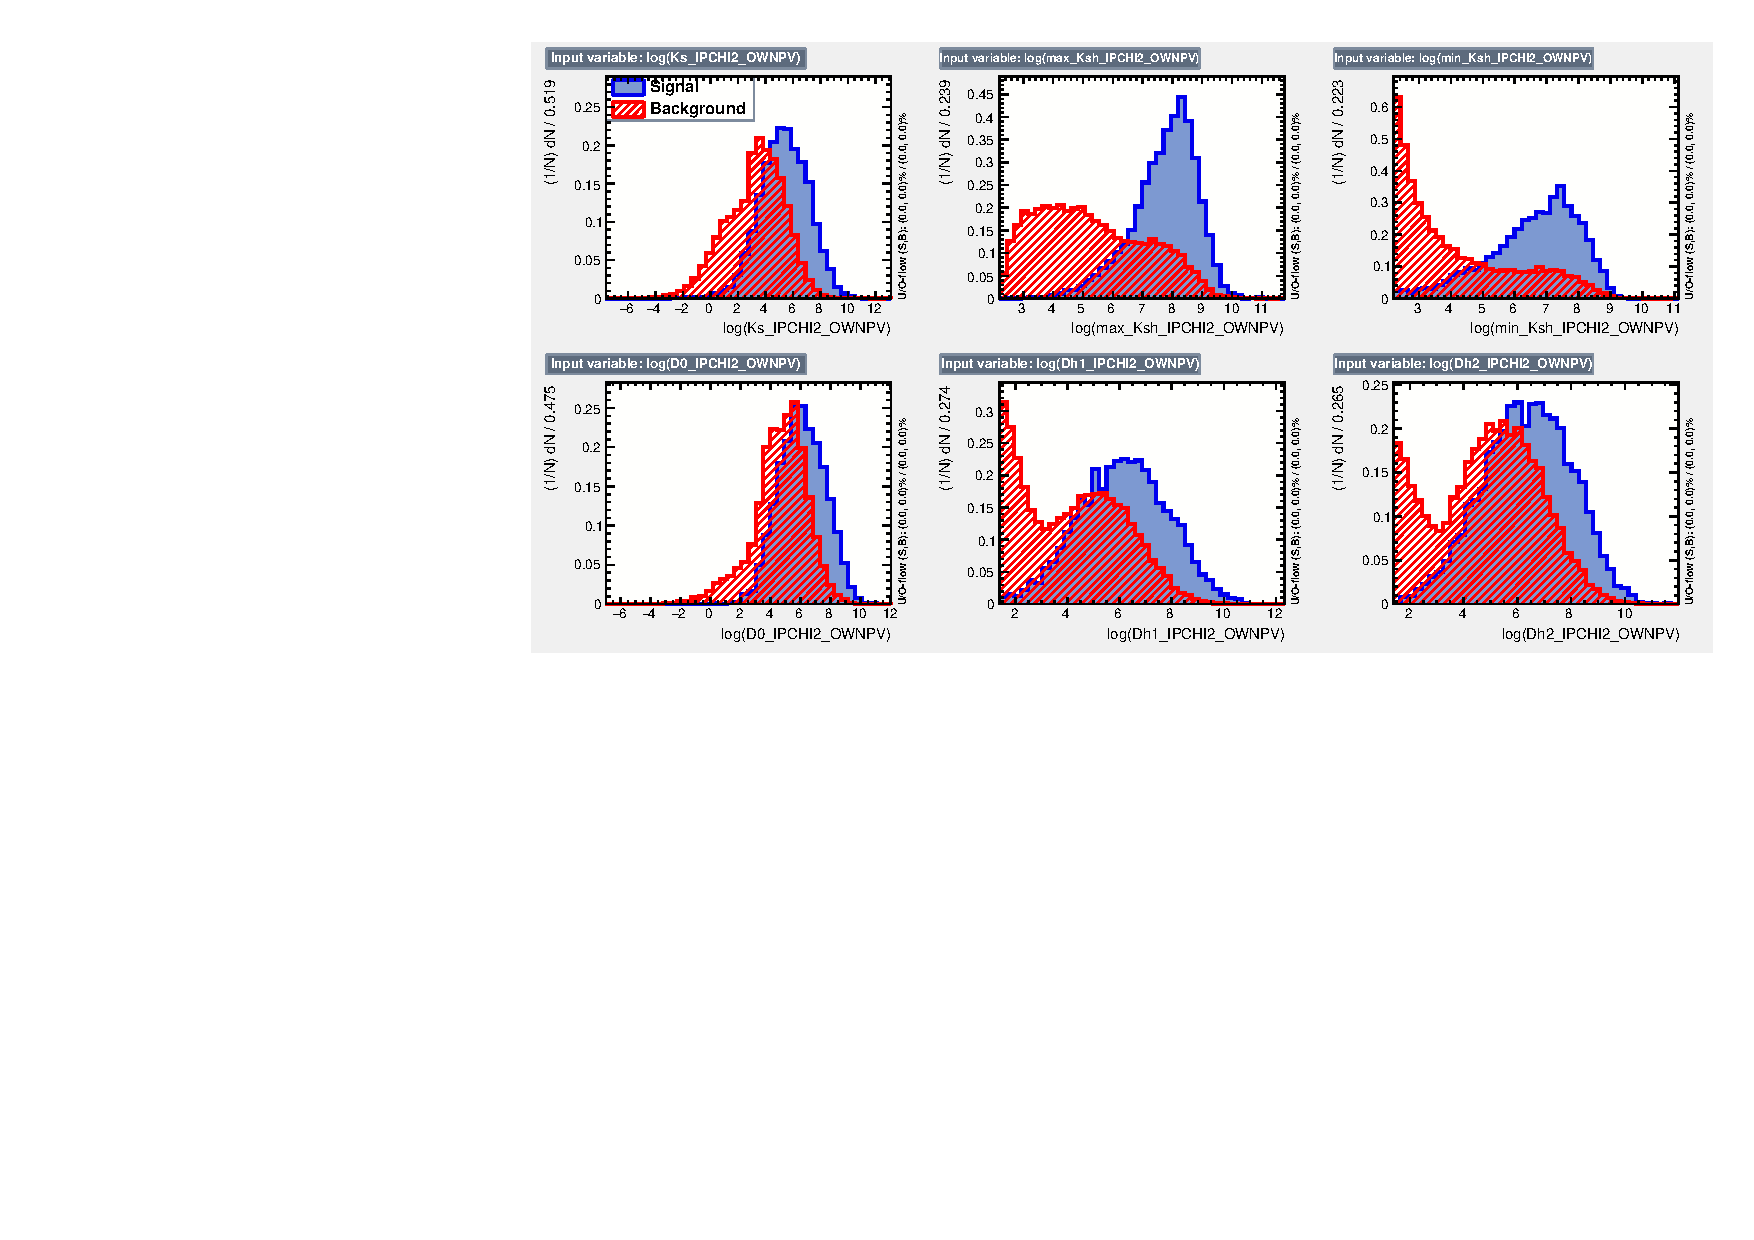
\includegraphics[width=\linewidth]{figures/selection/inputvariables_KPi_LL_run1_1.pdf}
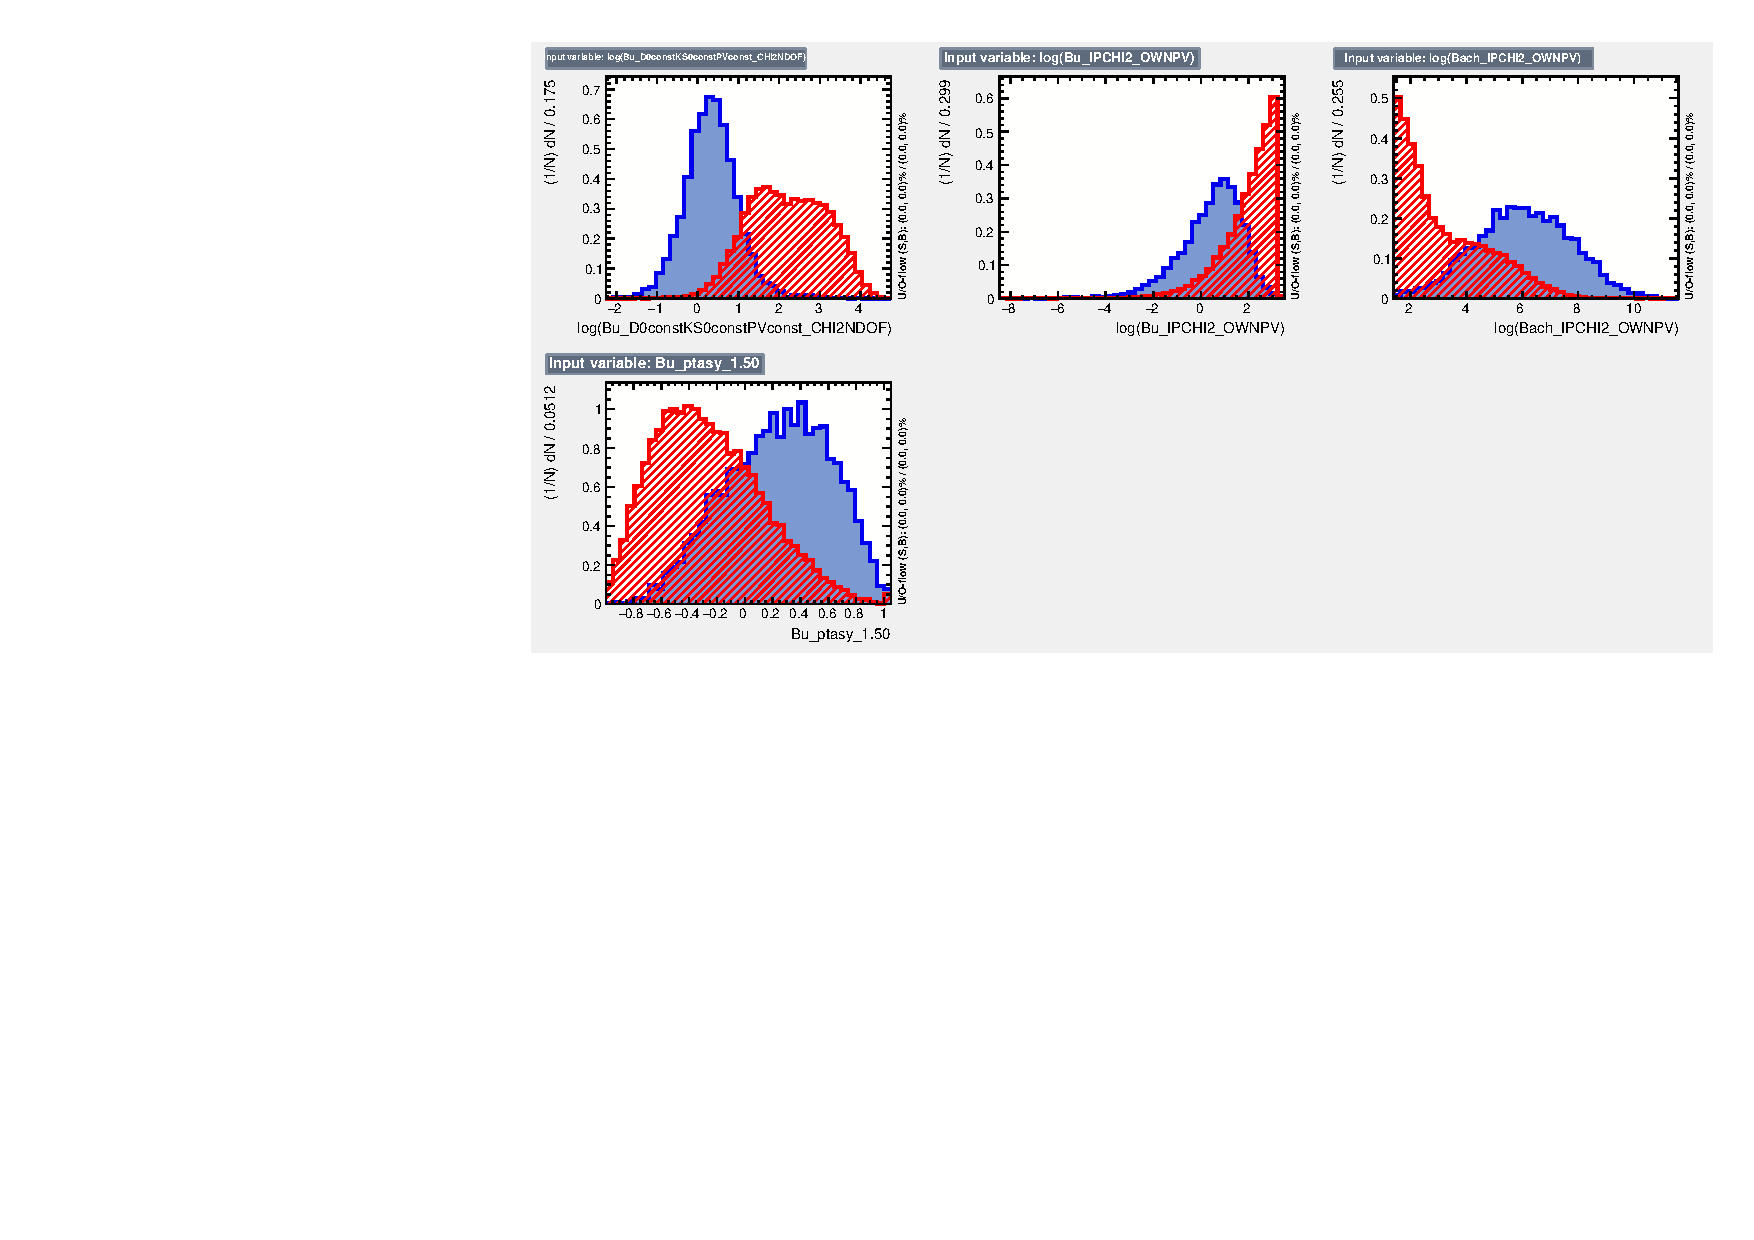
\includegraphics[width=\linewidth]{figures/selection/inputvariables_KPi_LL_run1_2.pdf}
\caption{Distributions of the input variables using the training signal and background samples for two-body LL BDT.}
\label{BDTinputdist2bodyLL}
\end{figure}

\begin{figure}
\centering
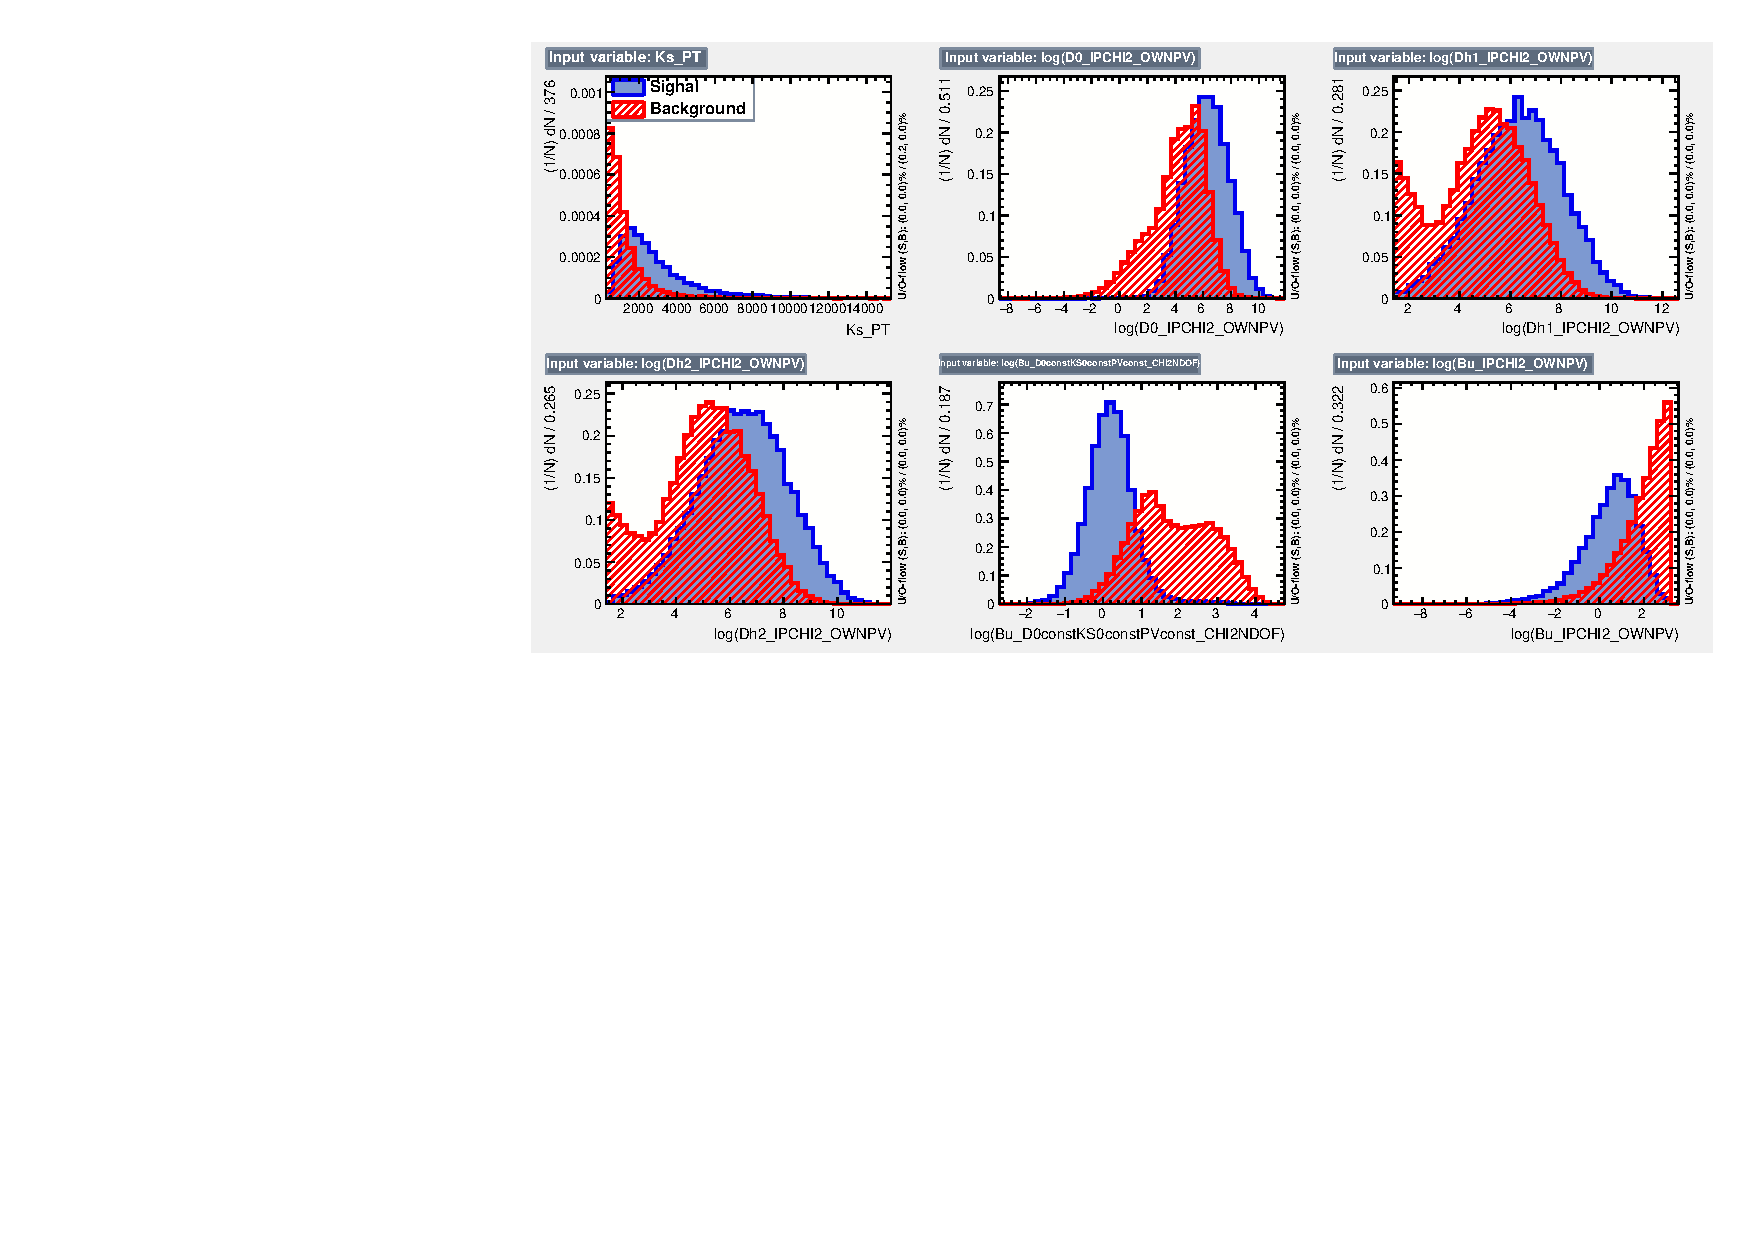
\includegraphics[width=\linewidth]{figures/selection/inputvariables_KPi_DD_run1_1.pdf}
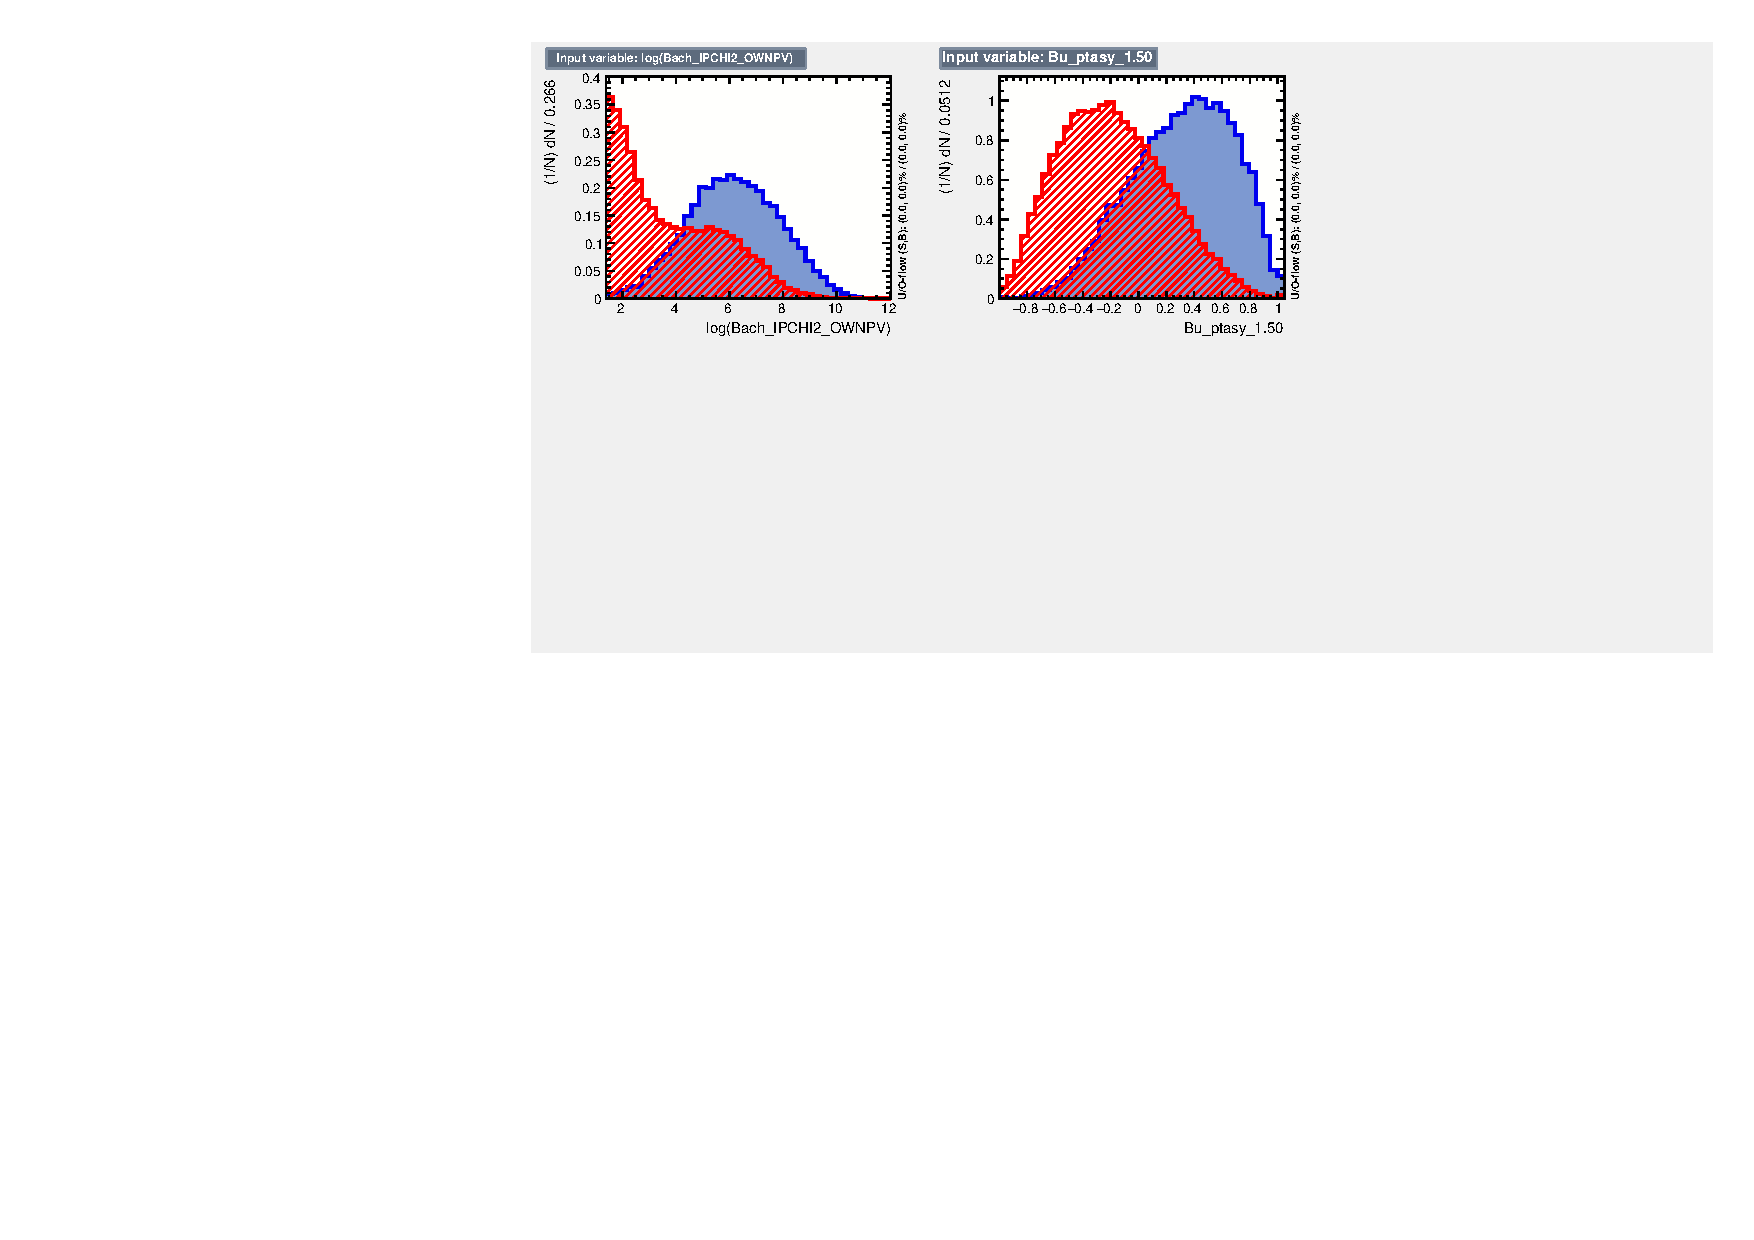
\includegraphics[trim = 0mm 50mm 0mm 0mm, clip,width=\linewidth]{figures/selection/inputvariables_KPi_DD_run1_2.pdf}
\caption{Distributions of the input variables using the training signal and background samples for two-body DD BDT.}
\label{BDTinputdist2bodyDD}
\end{figure}

\subsubsection{Performance of the multivariate algorithm and choice of working point}

Selections are optimised for minimising the uncertainty in the \CP observables. This method required the full fit and is described in Section \ref{sec:cpfit:optimisation}. The final BDT requirements chosen based on this optimisation are given in Table \ref{bdtrequirements}, and the signal and background efficiencies in the two- and four-body \Dz decay modes, for the chosen BDT requirements, are given in Tables \ref{BDTresults}. The performance of the two- and four-body BDTs, as well as LL and DD categories, are very similar. In all catergories the BDT has a signal efficiency above 90\% and a background efficiency of less than 6\%. 

\begin{table}
\centering
\begin{tabular}{c|cc}
 & LL & DD \\
\hline
All \Dz modes except the ADS modes & 0.6 & 0.7 \\
ADS modes & 0.6 & 0.9 \\
\end{tabular}
\caption{BDT requirements on each of the \Dz decay modes for both LL and DD candidates.}
\label{bdtrequirements}
\end{table}

\begin{table}
\centering
\begin{tabular}{c|cc}
& LL & DD \\
\hline
\kpi & 0.95 (0.06) & 0.90 (0.05) \\
\kpipipi & 0.95 (0.04) & 0.93 (0.03) \\
\end{tabular}
\caption{Signal and background efficiencies averaged across the whole dataset for the chosen BDT requirements in both \kpi and \kpipipi modes.}
\label{BDTresults}
\end{table}


\subsection{Summary of the selection requirements}

Table \ref{selectionsummary} lists a summary of the selection requirements applied in this analysis to select \btodkst decays and remove combinatorial background events as well as various peaking backgrounds. 

\begin{table}[h]
\centering
\resizebox{\textwidth}{!}{
\begin{tabular}{c|c}
\hline
\textbf{Variable} & \textbf{Selection requirement} \\
\hline \hline
\multicolumn{1}{l}{\textbf{Mass variables}} & \\
\hline \hline
$\textbar$ \Dz mass - 1864.86 \mevcc $\textbar$ & $<$ 25 \mevcc \\
$\textbar$ \KS mass - 497.614 \mevcc $\textbar$ & $<$ 15 \mevcc for LL, $<$ 20 \mevcc for DD \\
$\textbar$ \Kstarm mass - 892 \mevcc $\textbar$ & $<$ 75 \mevcc \\
\hline \hline
\multicolumn{1}{l}{\textbf{PID and veto}} & \\
\hline \hline
DLLK of bachelor & $<$ 4 \\
DLLK of D daughters (two-body) & $>$ 2 for all kaons, $<$ -2 for all pions \\
DLLK of D daughters (\decay{\Dz}{\Km\pip\pim\pip}) & $>$ 2 for \Km, $<$ -2 for both \pip mesons \\
DLLK of D daughters (\decay{\Dz}{\pim\pip\pim\pip}) & $<$ -2 for both \pip mesons \\
$\textbar \Dz_{swapped} - 1864.86 \mevcc \textbar$ for ADS modes & $>$ 15 \mevcc \\
\hline \hline
\multicolumn{1}{l}{\textbf{Other backgrounds}} & \\
\hline \hline
$\textbar \cos(\theta_{\KS}) \textbar$ & $>$ 0.3 \\
\Dz FD significance & $>$ 2 \\
\KS FD significance & $>$ 5 for LL, no requirement for DD \\
\Bm \chisqip & 0 - 25 \\
\Bm \chisq/dof & 0 - 100 \\
\hline \hline
\multicolumn{1}{l}{\textbf{BDT}} & \\
\hline \hline
BDT classifier for CF and GLW modes & $>$ 0.6 for LL, $>$ 0.7 for DD \\
BDT classifier for ADS modes & $>$ 0.6 for LL, $>$ 0.9 for DD \\
\hline
\end{tabular}}
\caption{Summary of the selection requirements applied in this analysis}
\label{selectionsummary}
\end{table}

\subsection{Final refitted \Bm mass distributions}

The reconstructed \Bm mass distributions, with constraints applied, for each of the samples passing the full selection requirements, detailed in this chapter, are given in Figure \ref{fig:finalBmass}.

\begin{figure}[h]
\centering
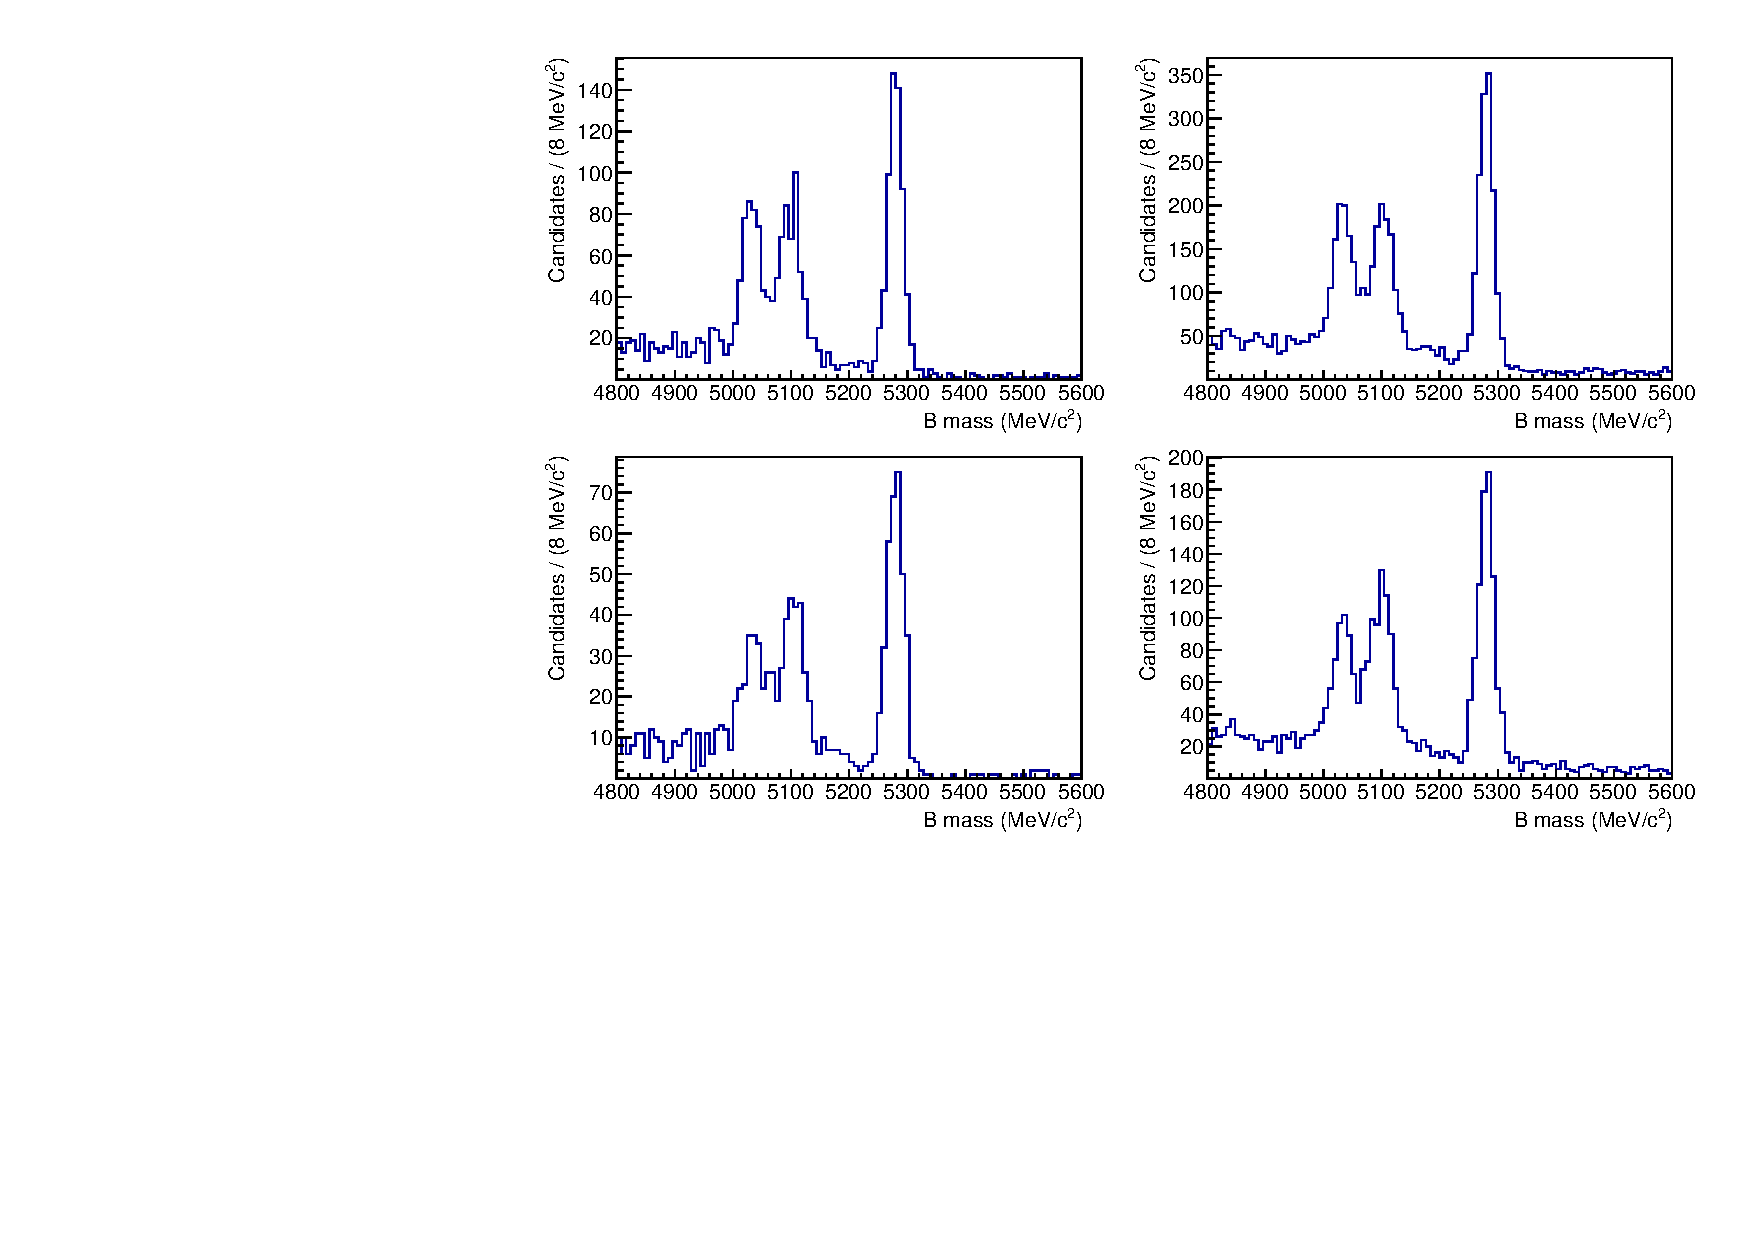
\includegraphics[width=0.8\linewidth]{figures/selection/finalBmass.pdf}
\put(-300,190) {(a)}
\put(-130,190) {(b)}
\put(-300,80) {(c)}
\put(-130,80) {(d)}
\caption{Refitted \Bm mass distributions after the full selection has been applied for (a) \kpi LL, (b) \kpi DD, (c) \kpipipi LL, and (d) \kpipipi DD candidates with \runone and \runtwo samples combined.}
\label{fig:finalBmass}
\end{figure}

\clearpage

\section{Mass parameterisation of the favoured modes}
\label{sec:massfit}

This section describes the \Bm mass parameterisation developed for the two- and four-body favoured \Dz modes, namely \kpi and \kpipipi. The aim is to first develop a model that parameterises the invariant \Bm mass, and then perform fits to the \kpi and \kpipipi data from which various parameters can be extracted. The model developed for the favoured \kpi and \kpipipi modes is applied to the suppressed \Dz decay modes when performing the simultaneous fit to measure the \CP observables, as described in Section \ref{ch:5-cpfit}. There are three components considered in the model to parameterise the \kpi and \kpipipi \Bm mass distributions:
\begin{enumerate}
\item Signal, \decay{\Bm}{\D\Kstarm} decays,
\item Combinatorial background, where random tracks are combined in the reconstruction ,
\item Partially reconstructed background, where one particle has been missed in the reconstruction, for example \decay{\Bm}{(\decay{\Dstarz}{\Dz[\piz]})\Kstarm}, where the \piz is not reconstructed.
\end{enumerate}

The shape of each component of the model, and any constraints in background yields imposed, are discussed in the following sections. Data samples are considered separately for LL and DD \KS reconstruction types as well as \runone and \runtwo data-taking periods. When developing the mass parameterisation of the \kpi and \kpipipi modes, these samples are considered separately unless the distributions were found not to be significantly different. It is expected that shapes for the LL and DD \KS reconstruction categories will be different due to their different reconstructed \Bm mass resolutions.

\subsection{Signal shape}
\label{sec:massfit:signal}

The signal shape is described as the sum of two Gaussians each with a tail extending towards lower invariant mass to account for radiative effects. These modified Gaussians are known as Crystal Ball (CB) functions~\cite{Skwarnicki:1986xj}. This Double Crystal Ball shape used is defined by,
\begin{equation}
\mathrm{DCB}(m| \mu,\sigma,\alpha,n,f_{cb}) = f_{cb} \cdot \mathrm{CB}(m| \mu,\sigma,\alpha,n) + (1-f_{cb}) \cdot \mathrm{CB}(m|\mu,f_{\sigma}\sigma,\alpha,n),
\label{DCBshape}
\end{equation}
where
\begin{equation*}
  \mathrm{CB}(m| \mu,\sigma,\alpha,n)=
\begin{cases}
    e^{-((m-\mu)/ \sigma)^2/2},                                   & \text{if } \frac{m-\mu}{\sigma} \geq - \alpha, \\
   \left ( \frac{n}{|\alpha|} \right ) ^n e^{-|\alpha|^2/2} \left ( \frac{n}{|\alpha|} - |\alpha| - \left ( \frac{m-\mu}{\sigma} \right ) \right ) ^{-n} ,    & \text{otherwise.}
\end{cases}
\end{equation*}
where $\mu$ is the peak position, $\sigma$ is the width of the Gaussian, $n$ parameterises the power-law tail, which starts $\alpha\sigma$ away from the peak position. The parameters $f_{cb}$ and $(1-f_{cb})$ are the fraction of the yield given to each CB and $f_{\sigma}$ is the ratio of the widths between the two CBs.

%The fitted signal shape for the \runone and \runtwo data-taking samples, as well as the \kpi and \kpipipi modes were investigated to compare the shapes across different categories. Figure \ref{signalfitcomparison2body} shows comparisons of the resulting signal PDFs after fits to the \Bm mass distributions of simulated samples between \runone and \runtwo data-taking periods. These shapes are consistent between \runone and \runtwo, therefore signal shapes in different data-taking periods are shared in the simultaneous fit. Further comparisons are made between two- and four-body modes. Figure \ref{signalfitcomparisonRun1} compares the signal PDFs obtained from simulated samples between \kpi and \kpipipi for \runone samples. These are found to be significantly different and so \kpi and \kpipipi are associated with different signal shapes in the simultaneous fit.
The \Bm mass distributions from simulated signal events were found to be consistent between \runone and \runtwo data samples, but significantly different for \kpi and \kpipipi modes. Therefore the signal shape for different data-taking periods is the same, but different between \kpi and \kpipipi modes. 

%\begin{figure}[h]
%\centering
%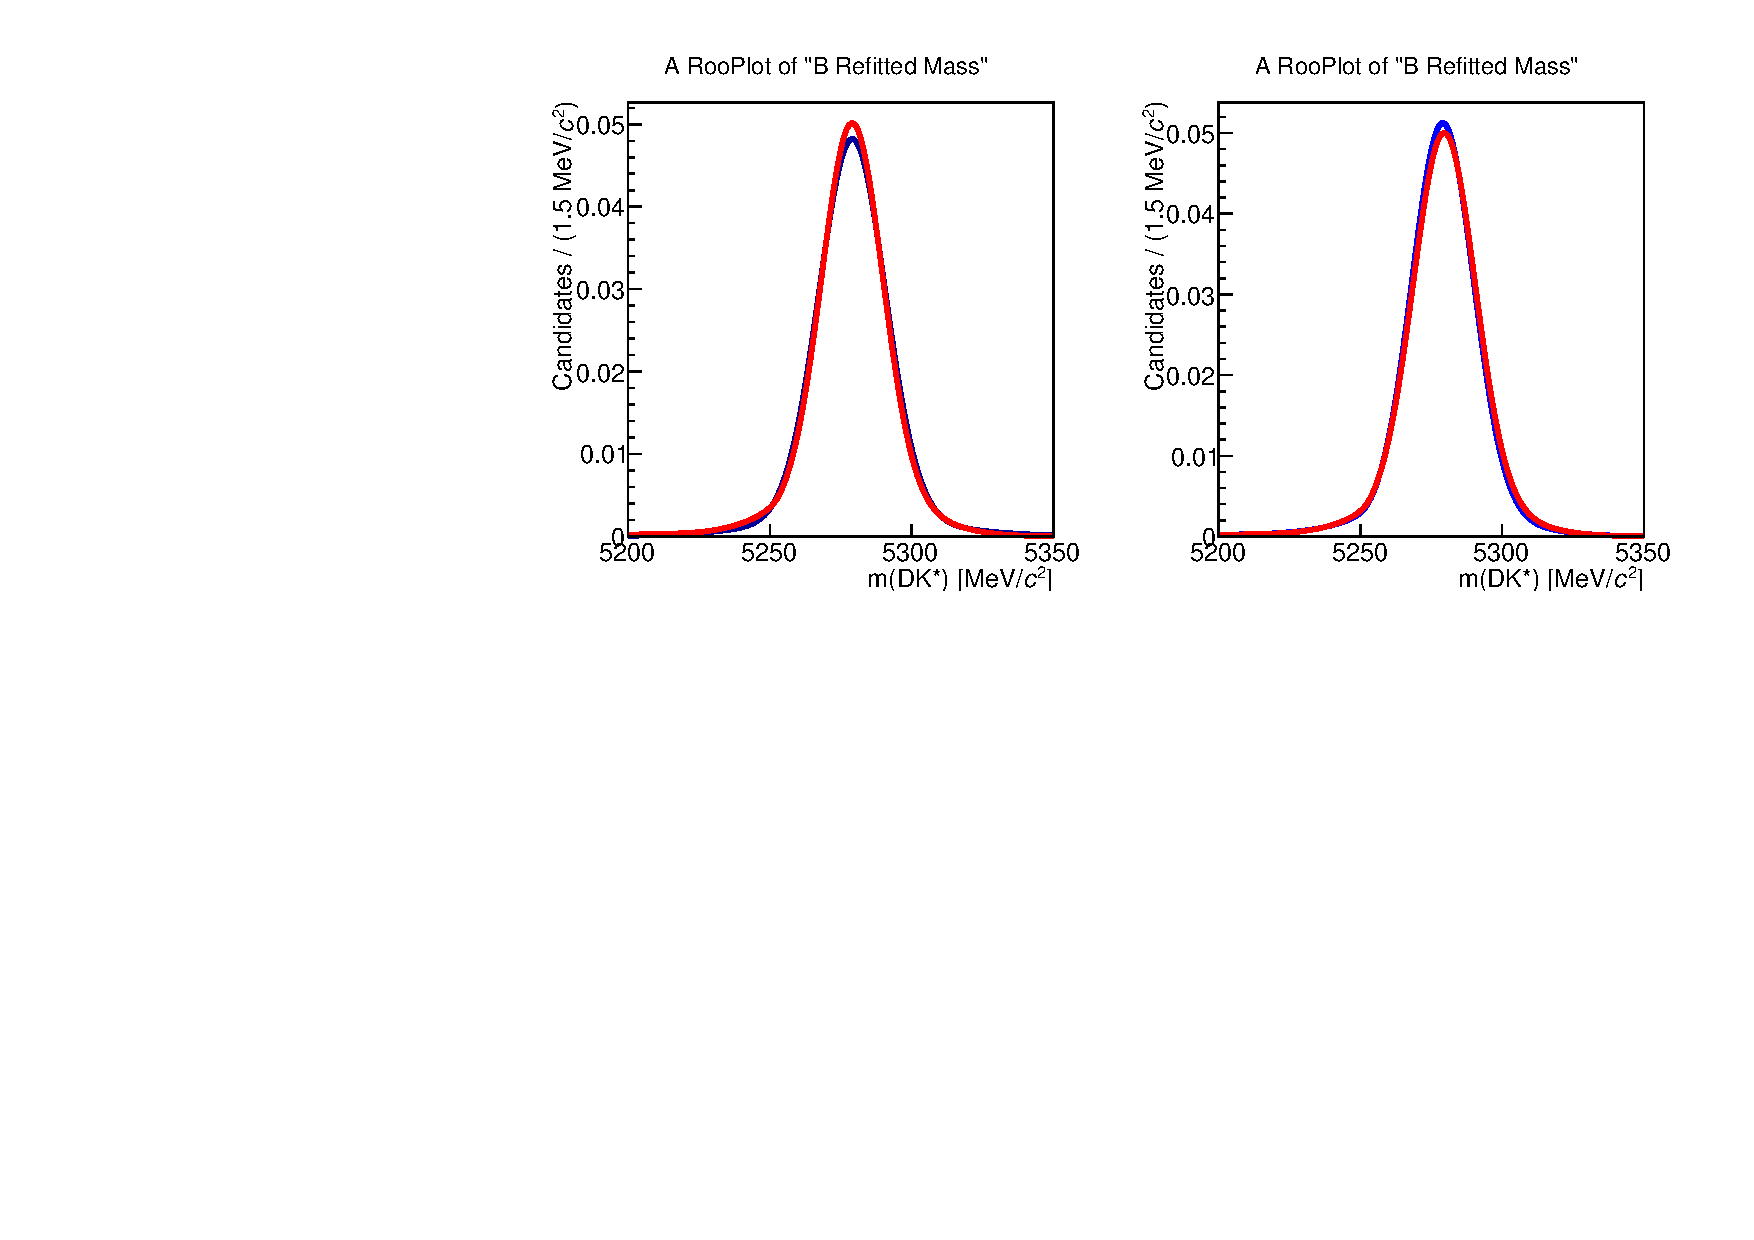
\includegraphics[width=0.7\linewidth]{figures/fitComponents/signalMC_KPi_run1vsrun2.pdf}
%\put(-260,100) {(a)}
%\put(-110,100) {(b)}
%\caption{Comparison of \kpi signal fit functions for \runone (blue) and \runtwo simulated samples (red) for (a) LL candidates and (b) DD candidates.}
%\label{signalfitcomparison2body}
%\end{figure}
%
%\begin{figure}[h]
%\centering
%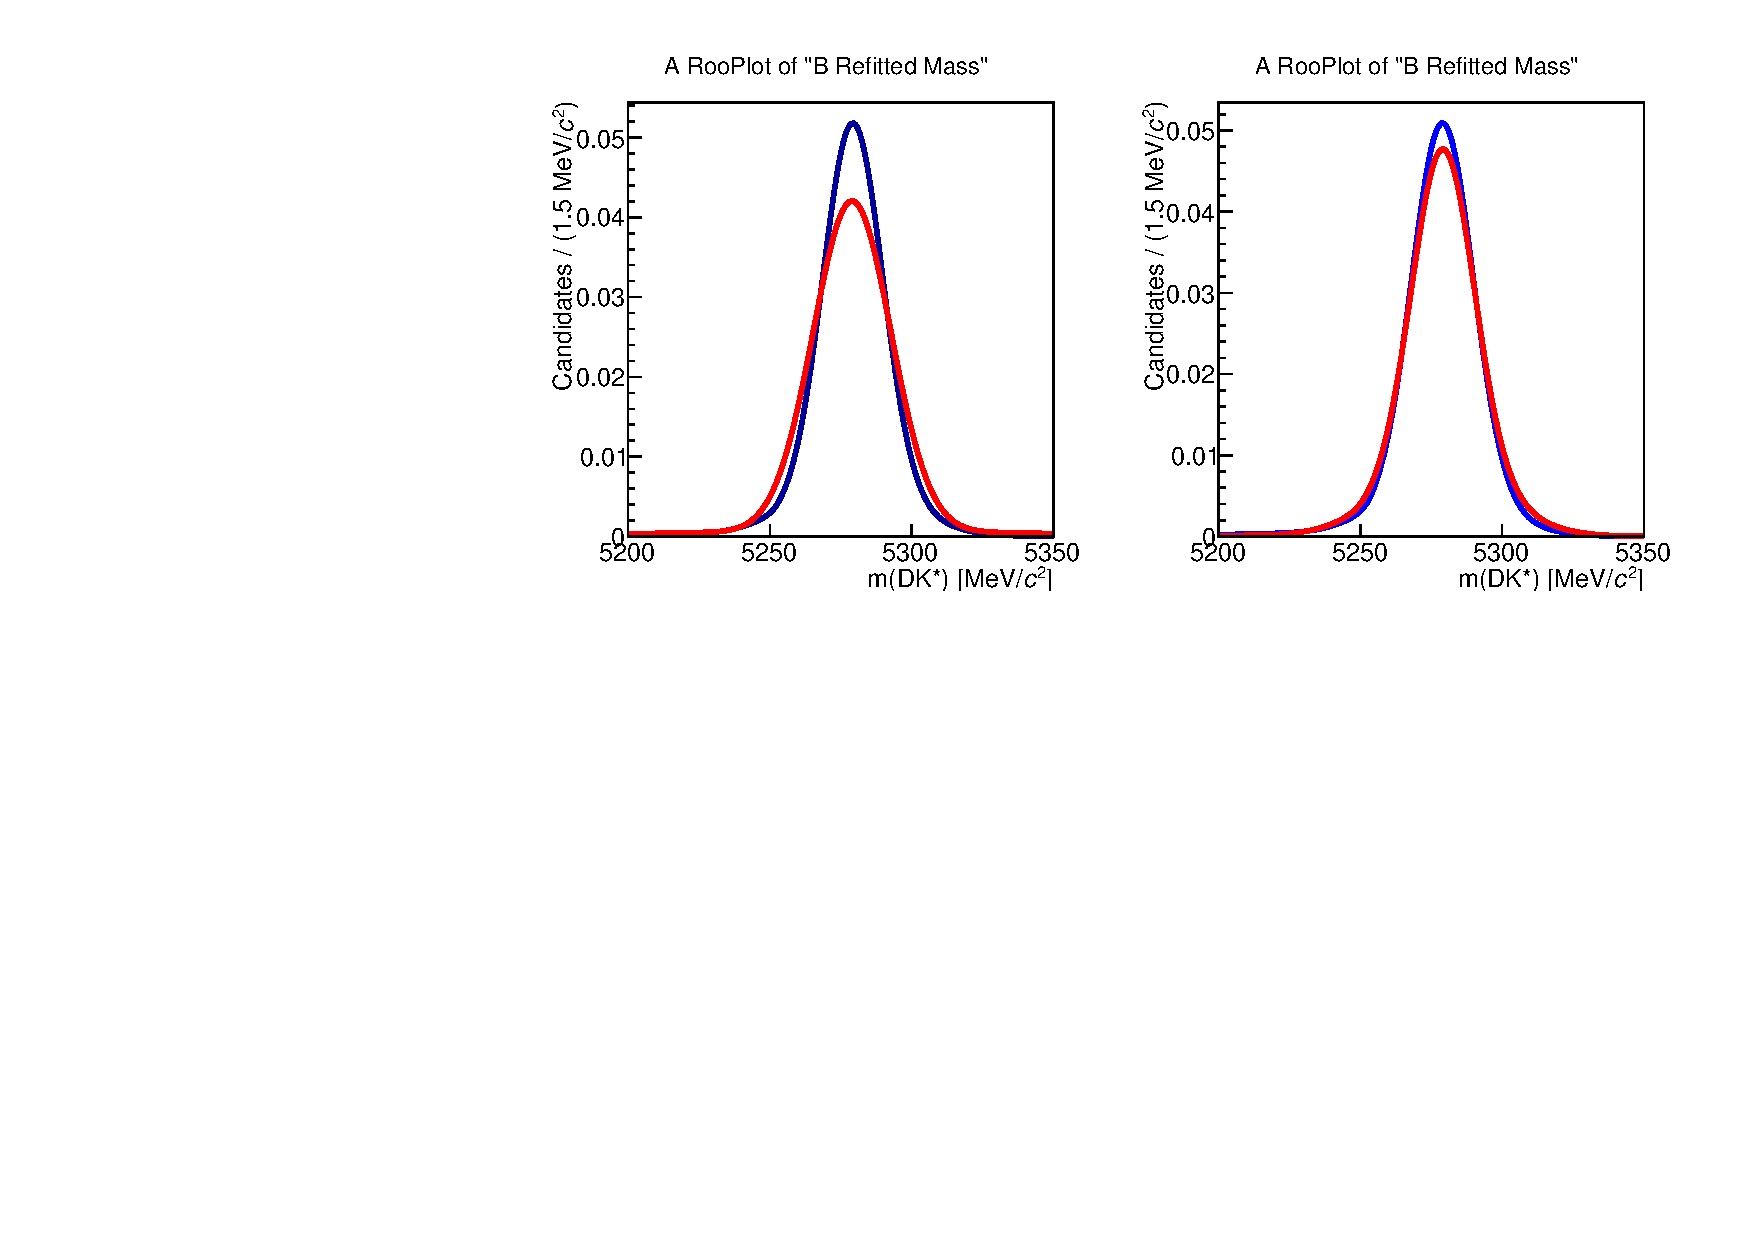
\includegraphics[width=0.7\linewidth]{figures/fitComponents/signalMC_run1_KPivsKPiPiPi.pdf}
%\put(-260,100) {(a)}
%\put(-110,100) {(b)}
%\caption{Comparison of \runone signal fit functions for \kpi (blue) and \kpipipi (red) simulated samples for (a) LL candidates and (b) DD candidates.}
%\label{signalfitcomparisonRun1}
%\end{figure}

The fits to simulated signal samples are shown in Figure \ref{signalfits} and the shape parameters obtained from these fits are detailed in Table \ref{signalparameters}. For the signal shape in the mass fit to the \kpi and \kpipipi modes, the tail parameters, $\alpha$ and $n$, are fixed from simulation and both CBs share the same peak position and tail parameters. The ratio of the widths between the CBs, $f_{\sigma}$, is fixed from simulation, but the peak position and width, $\mu$ and $\sigma$, are allowed to vary.

\begin{figure}[h]
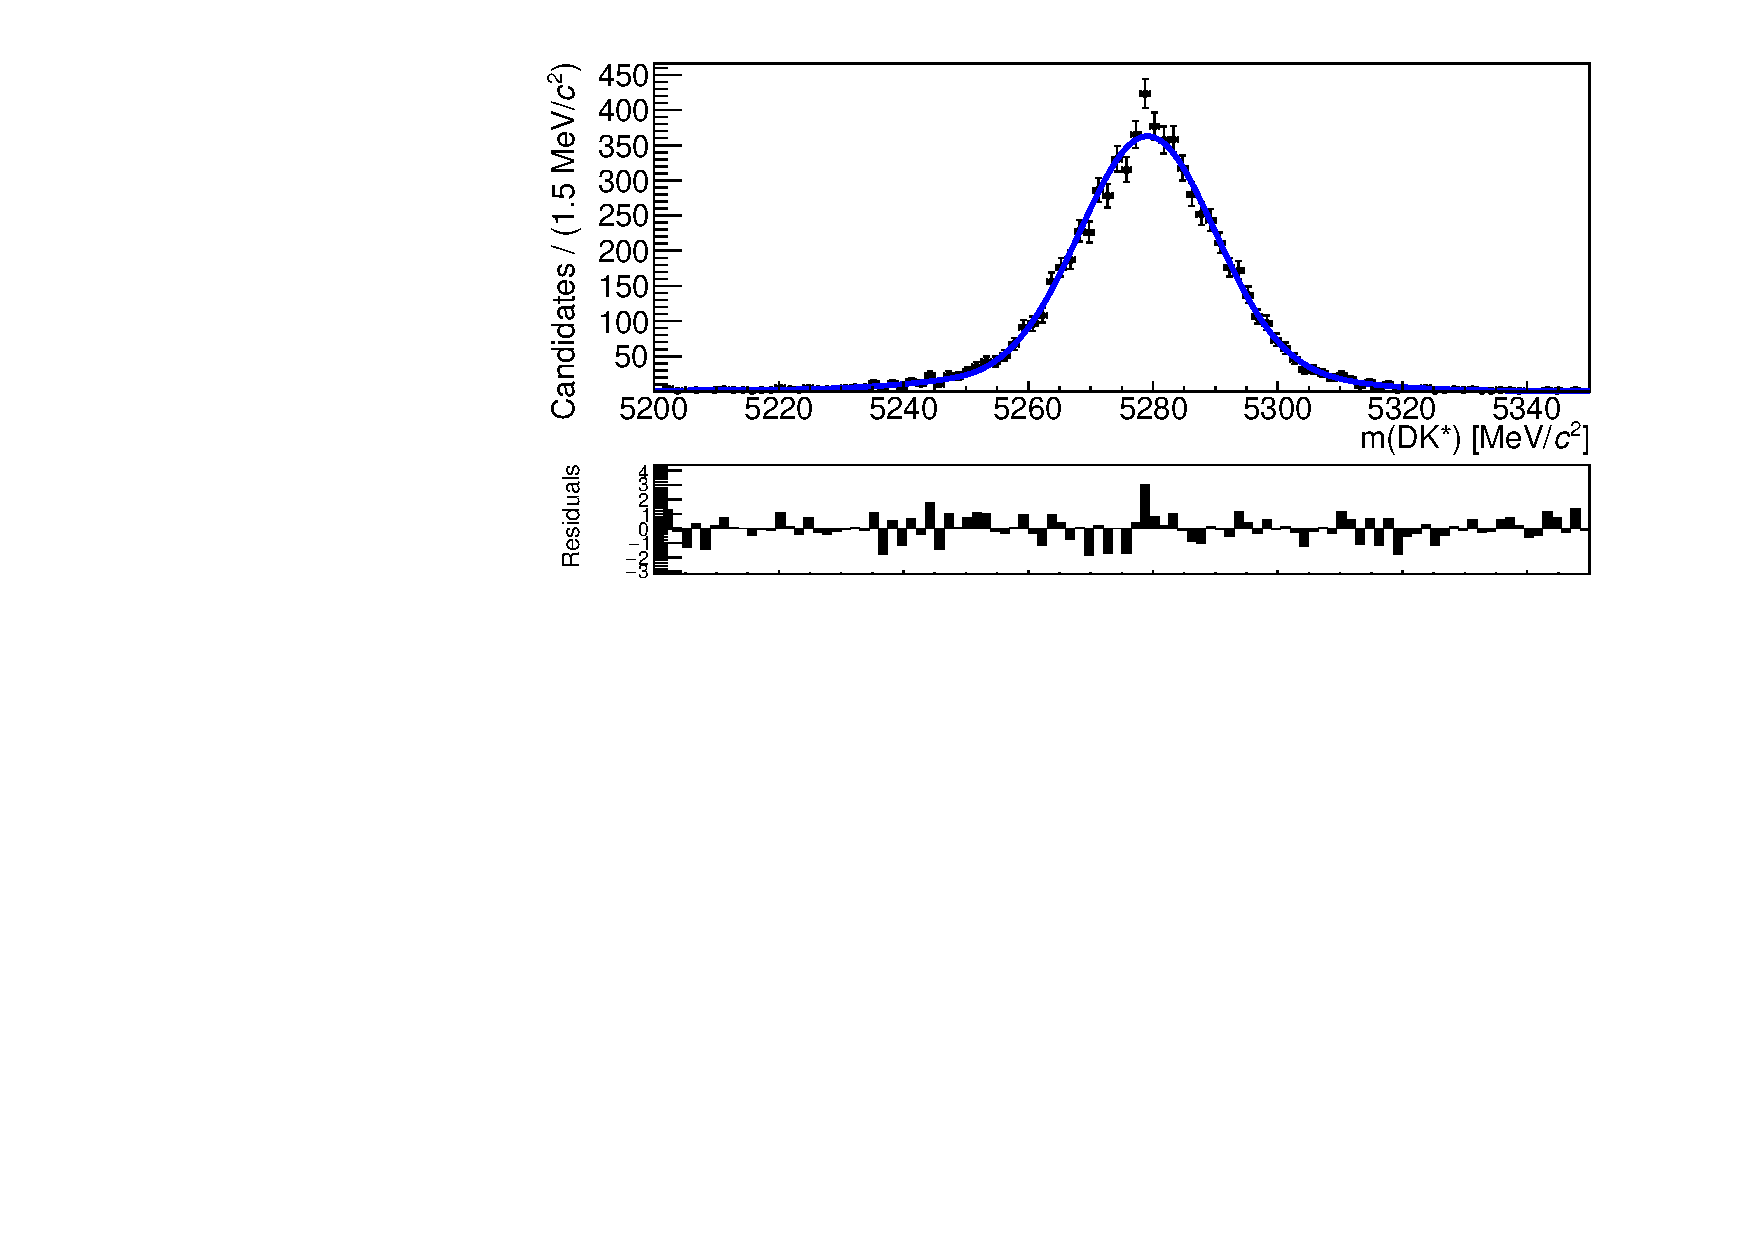
\includegraphics[width=0.5\linewidth]{figures/fitComponents/signalShape_LL_KPi.pdf}
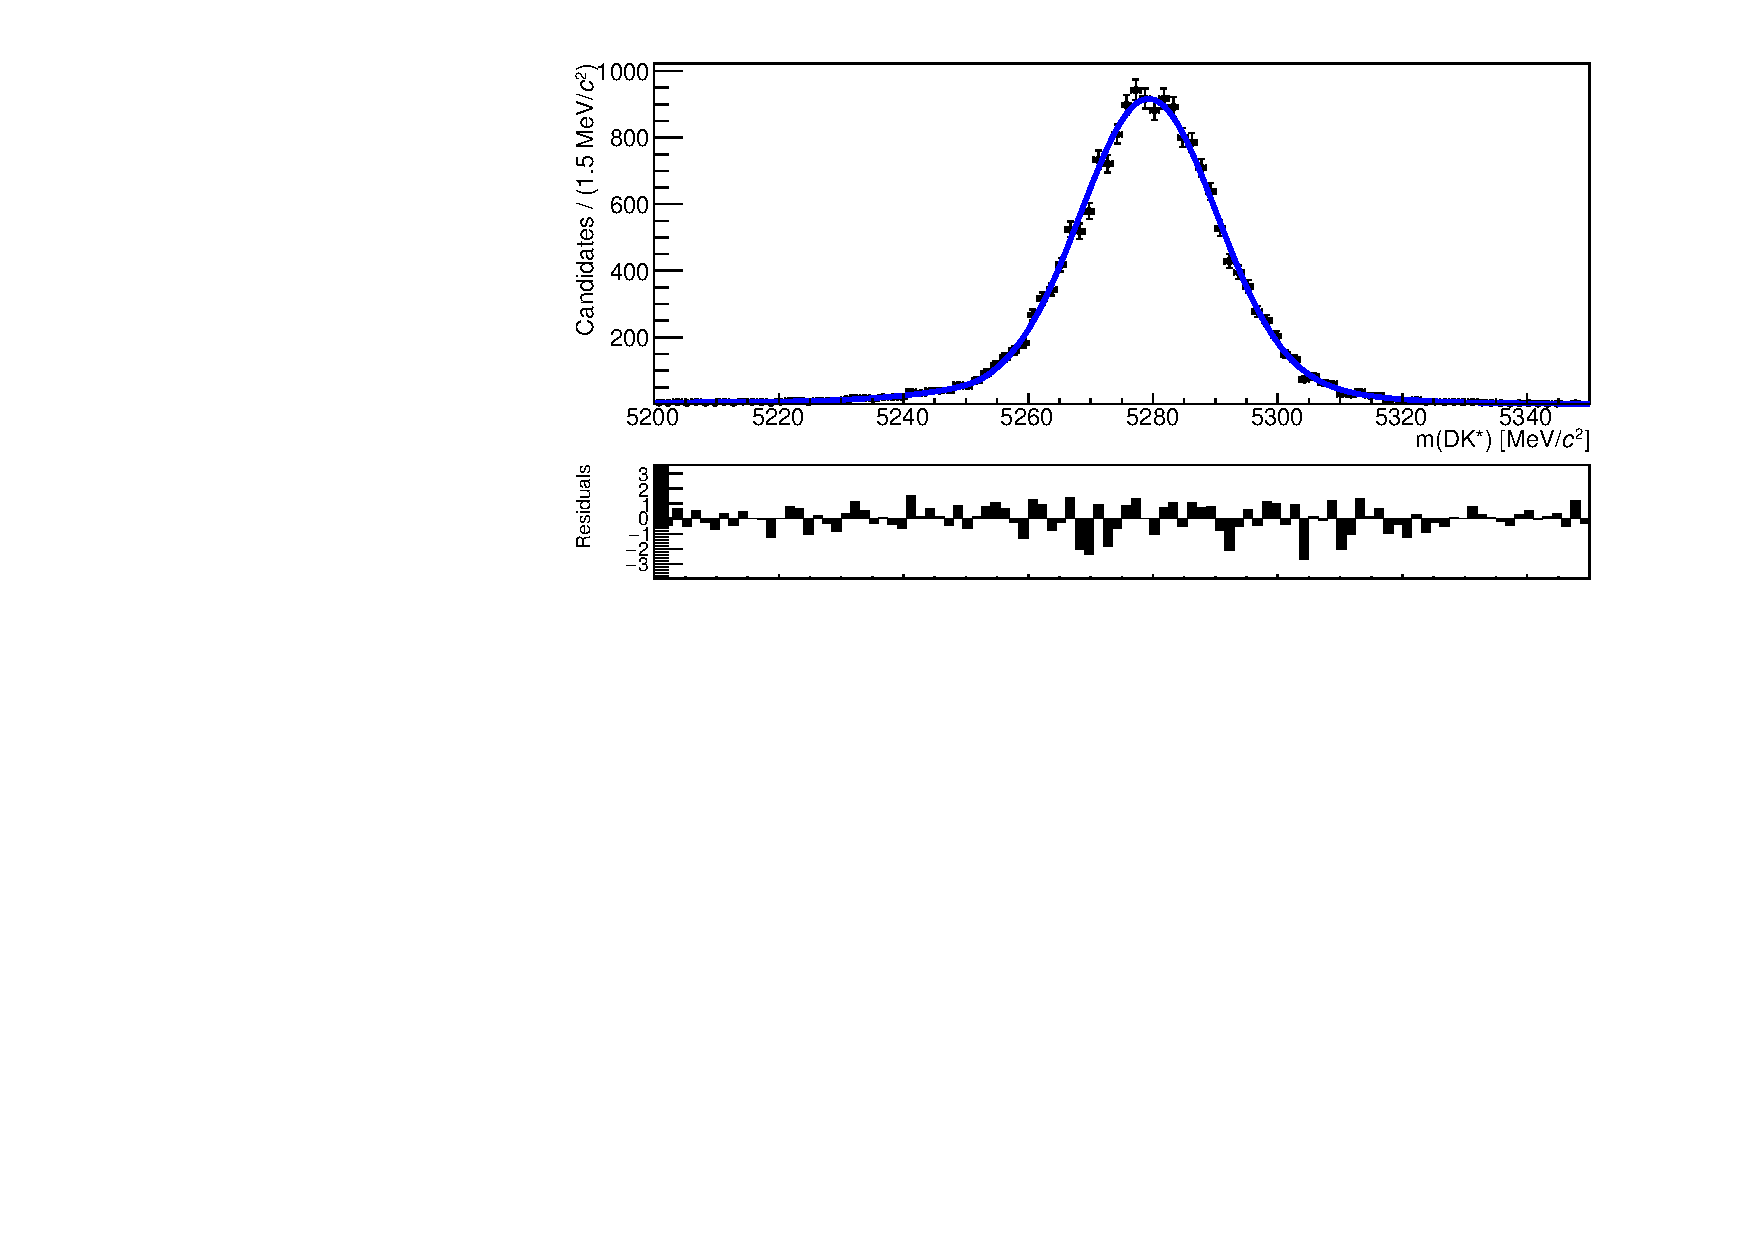
\includegraphics[width=0.5\linewidth]{figures/fitComponents/signalShape_DD_KPi.pdf}
\put(-390,70) {(a)}
\put(-180,70) {(b)}
\hfill
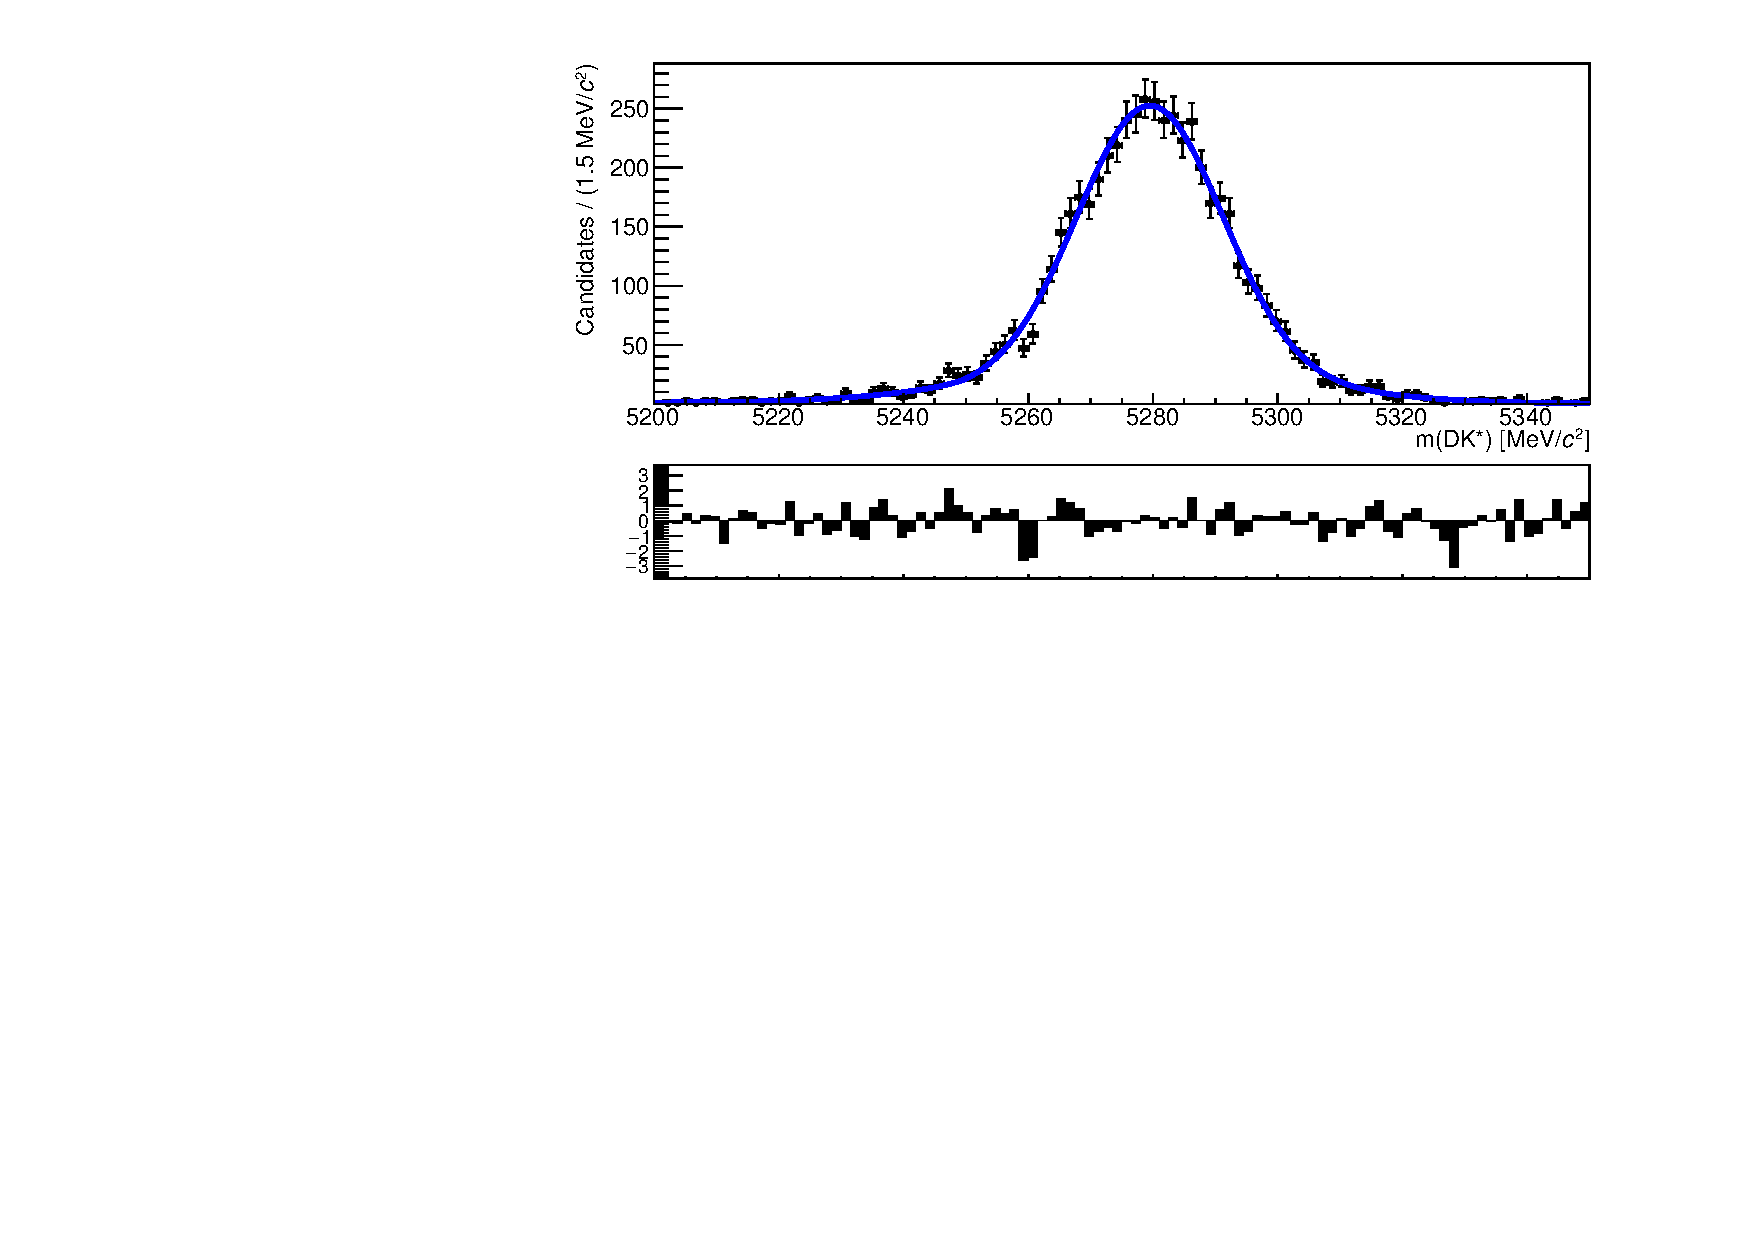
\includegraphics[width=0.5\linewidth]{figures/fitComponents/signalShape_LL_KPiPiPi.pdf}
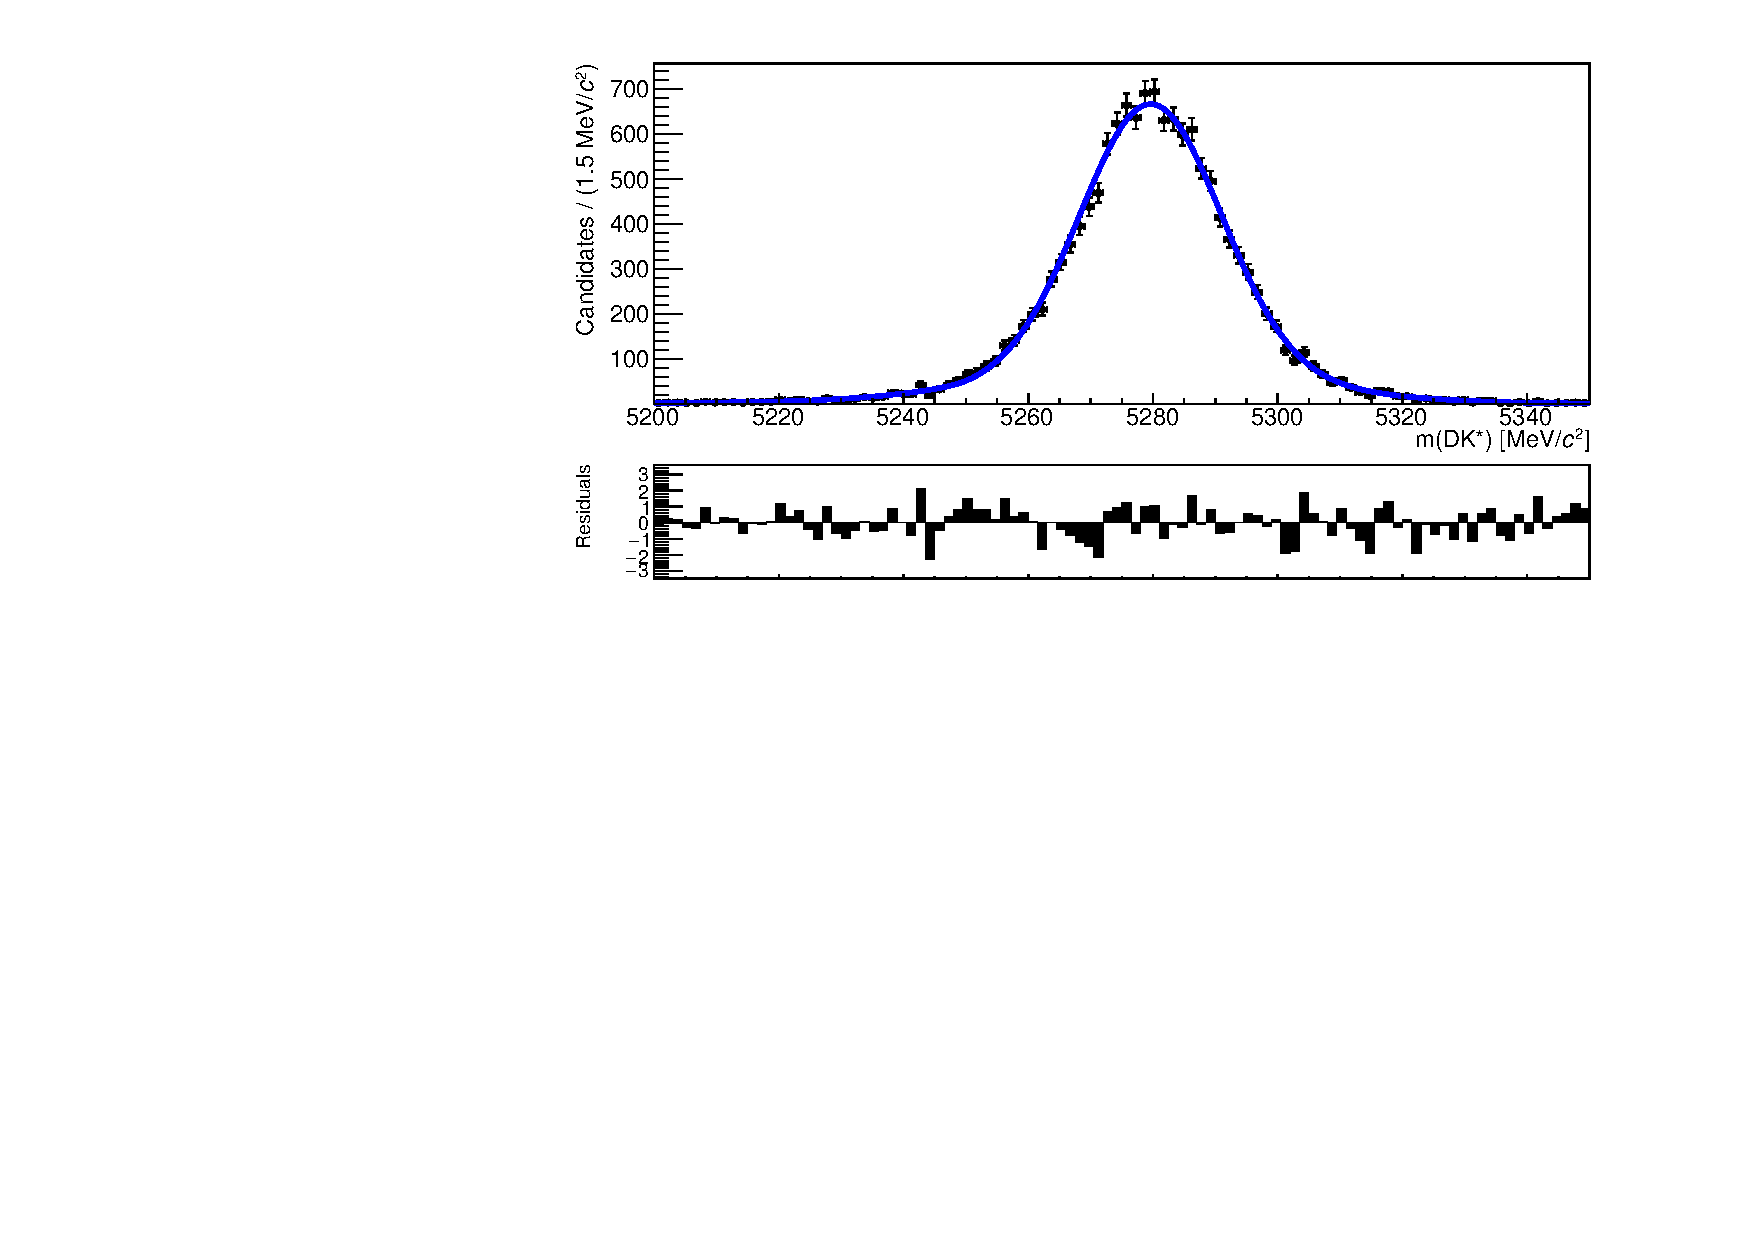
\includegraphics[width=0.5\linewidth]{figures/fitComponents/signalShape_DD_KPiPiPi.pdf}
\put(-390,70) {(c)}
\put(-180,70) {(d)}
\caption{Fits to the \Bm mass distribution from simulated signal samples with \runone and \runtwo data combined for (a) \kpi LL, (b) \kpi DD, (c) \kpipipi LL, and (d) \kpipipi DD.}
\label{signalfits}
\end{figure}

\begin{table}[h]
\centering
\begin{tabular}{c|cc|cc}
\hline
& \multicolumn{2}{c}{\kpi} & \multicolumn{2}{c}{\kpipipi} \\
& LL & DD & LL & DD\\
\hline
$\mu$ & $5279.12 \pm 0.15$ & $5279.30 \pm 0.09$ & $5279.62 \pm 0.12$ & $5279.50 \pm 0.19$ \\
$\sigma$ & $10.7 \pm 0.3$ & $10.8 \pm 0.2$ & $11.2 \pm 0.2$ & $11.6 \pm 0.3$ \\
$f_{\sigma}$ & $2.04 \pm 0.10$ & $1.97 \pm 0.06$ & $2.08 \pm 0.07$ & $2.10 \pm 0.11$ \\
$\alpha$ & $2.53 \pm 0.07$ & $2.46 \pm 0.04$ & $2.60 \pm 0.07$ & $2.50 \pm 0.10$ \\
$n$ & 1.0 (fixed) & 1.0 (fixed) & 1.0 (fixed) & 1.0 (fixed) \\
$f_{cb}$ & $0.82 \pm 0.03$ & $0.84 \pm 0.02$ & $0.80 \pm 0.03$ & $0.81 \pm 0.04	$ \\
\hline
\end{tabular}
\caption{Signal shape parameters obtained by a fit to simulated signal samples of the \kpi and \kpipipi modes with \runone and \runtwo samples combined. Parameter names are defined in Equation \ref{DCBshape}. All parameters except for the peak position and width are fixed to these values in the mass fit.}
\label{signalparameters}
\end{table}


\subsection{Combinatorial background}
\label{sec:massfit:combinatorial}

The combinatorial background is formed of random tracks that do not correspond to the signal decay, being combined in the reconstruction, for example, random kaon and pion tracks in the detector incorrectly reconstructed to form a \Dz meson. The combinatorial background is modelled using an exponential function, given by $e^{\beta m}$, with a slope parameter, $\beta$, and yield that are allowed to vary. 
%The slope parameter is allowed to vary independently in the LL and DD categories and between two and four-body \Dz final states. Each \Dz final state can have a different combinatoric rate.


%%%%%%%%%%%%%%%%%%%%%%
\subsection{Partially reconstructed backgrounds}
\label{sec:massfit:partreco}

Partially reconstructed decays refer to those in which one or more particle has failed to be reconstructed, resulting in peaking structures in the \B mass spectrum at a reconstructed mass below the signal peak. 
%These decays are parameterised by analytic functions based on a previous studies of \decay{\Bm}{\D\Km}, \decay{\D}{h^+h^-} decays~\cite{LHCb-PAPER-2016-003} and \decay{\Bz}{\D\Kstarz}, \decay{\D}{h^+h^-} decays~\cite{LHCb-PAPER-2016-006}, which have many similar aspects to this analysis.

The partially reconstructed decays in this analysis are of the form \decay{\B}{\Dstar\Kstar}, where the \Dstar decays to a \Dz meson and a pion or photon that is missed when reconstructing the decay. These backgrounds are observed at a reconstructed invariant mass below the signal peak due to the single particle missed from the invariant mass sum. Three partially reconstructed decays contribute to the invariant mass fit:

\begin{itemize}
\item{\decay{\Bm}{(\decay{\Dstarz}{\Dz[\piz]})\Kstarm}}
\item{\decay{\Bm}{(\decay{\Dstarz}{\Dz[\gamma]})\Kstarm}}
\item{\decay{\Bd}{(\decay{\Dstarp}{\Dz[\pip]})\Kstarm}}
\end{itemize}

where the particle in square brackets corresponds to the missed particle. Each \decay{\B}{\Dstar\Kstar} decay is a Scalar $\to$ Vector Vector decay, therefore due to the conservation of angular momentum there are three different helicity amplitudes to consider. Each of these helicity amplitudes produces a \Dstar particle in a different helicity state, labelled +1, 0, -1. The helicity state of the \Dstar and the spin of the missing particle in the subsequent \Dstar decay determines the distribution of the reconstructed \B mass. The helicity states +1 and -1 produce the same distribution in \Bm mass, therefore for the mass parameterisation these states are combined and collectively referred to as $\pm$1. There are the 0 and $\pm$1 \Dstar helicity states for each of the three partially reconstructed decay modes, which results in six different shapes to be modelled in the mass fit:
\begin{itemize}
\item{\decay{\Bm}{(\decay{\Dstarz}{\Dz[\piz]})\Kstarm}, \Dstarz helicity: 0} 
\item{\decay{\Bm}{(\decay{\Dstarz}{\Dz[\piz]})\Kstarm}, \Dstarz helicity: $\pm$1} 
\item{\decay{\Bm}{(\decay{\Dstarz}{\Dz[\gamma]})\Kstarm}, \Dstarz helicity: 0}
\item{\decay{\Bm}{(\decay{\Dstarz}{\Dz[\gamma]})\Kstarm}, \Dstarz helicity: $\pm$1}
\item{\decay{\Bd}{(\decay{\Dstarp}{\Dz[\pip]})\Kstarm}, \Dstarp helicity: 0}
\item{\decay{\Bd}{(\decay{\Dstarp}{\Dz[\pip]})\Kstarm}, \Dstarp helicity: $\pm$1}
\end{itemize}
All of these shapes are modelled using three analytic probability density functions; Horns, Hill and Little Horns, developed by Paolo Gandini and Shu-Faye Cheung. These shapes, described in the following sections, are physically motivated, exploiting the decay kinematics of these partially reconstructed decays.

\subsubsection{Horns function}

Consider the \decay{\Bm}{\Dstarz\Kstarm}, \decay{\Dstarz}{\Dz\piz}, where the \Dstarz is in helicity state 0. The helicity of the \Dstarz, the fact that the missing \piz meson is spin-0 and the requirement that angular momentum must be conserved mean that the \piz meson will decay predominantly along $\theta = 0^{\circ}$ or $\theta = 180^{\circ}$. When $\theta = 0^{\circ}$, the fraction of momentum carried by the \piz in the \Bm rest frame is at its smallest, resulting in a larger reconstructed \Bm mass. Conversely, if $\theta = 180^{\circ}$, the fraction of momentum carried by the \piz is greatest, leading to a lower reconstructed \Bm mass. The distribution of the helicity angle of the missing particle, $\theta$, has a one-to-one correspondence with its momentum and therefore the reconstructed \Bm mass. This gives rise to a double peak structure, as shown in Figure \ref{fig:horns}.

\begin{figure}[h]
\centering
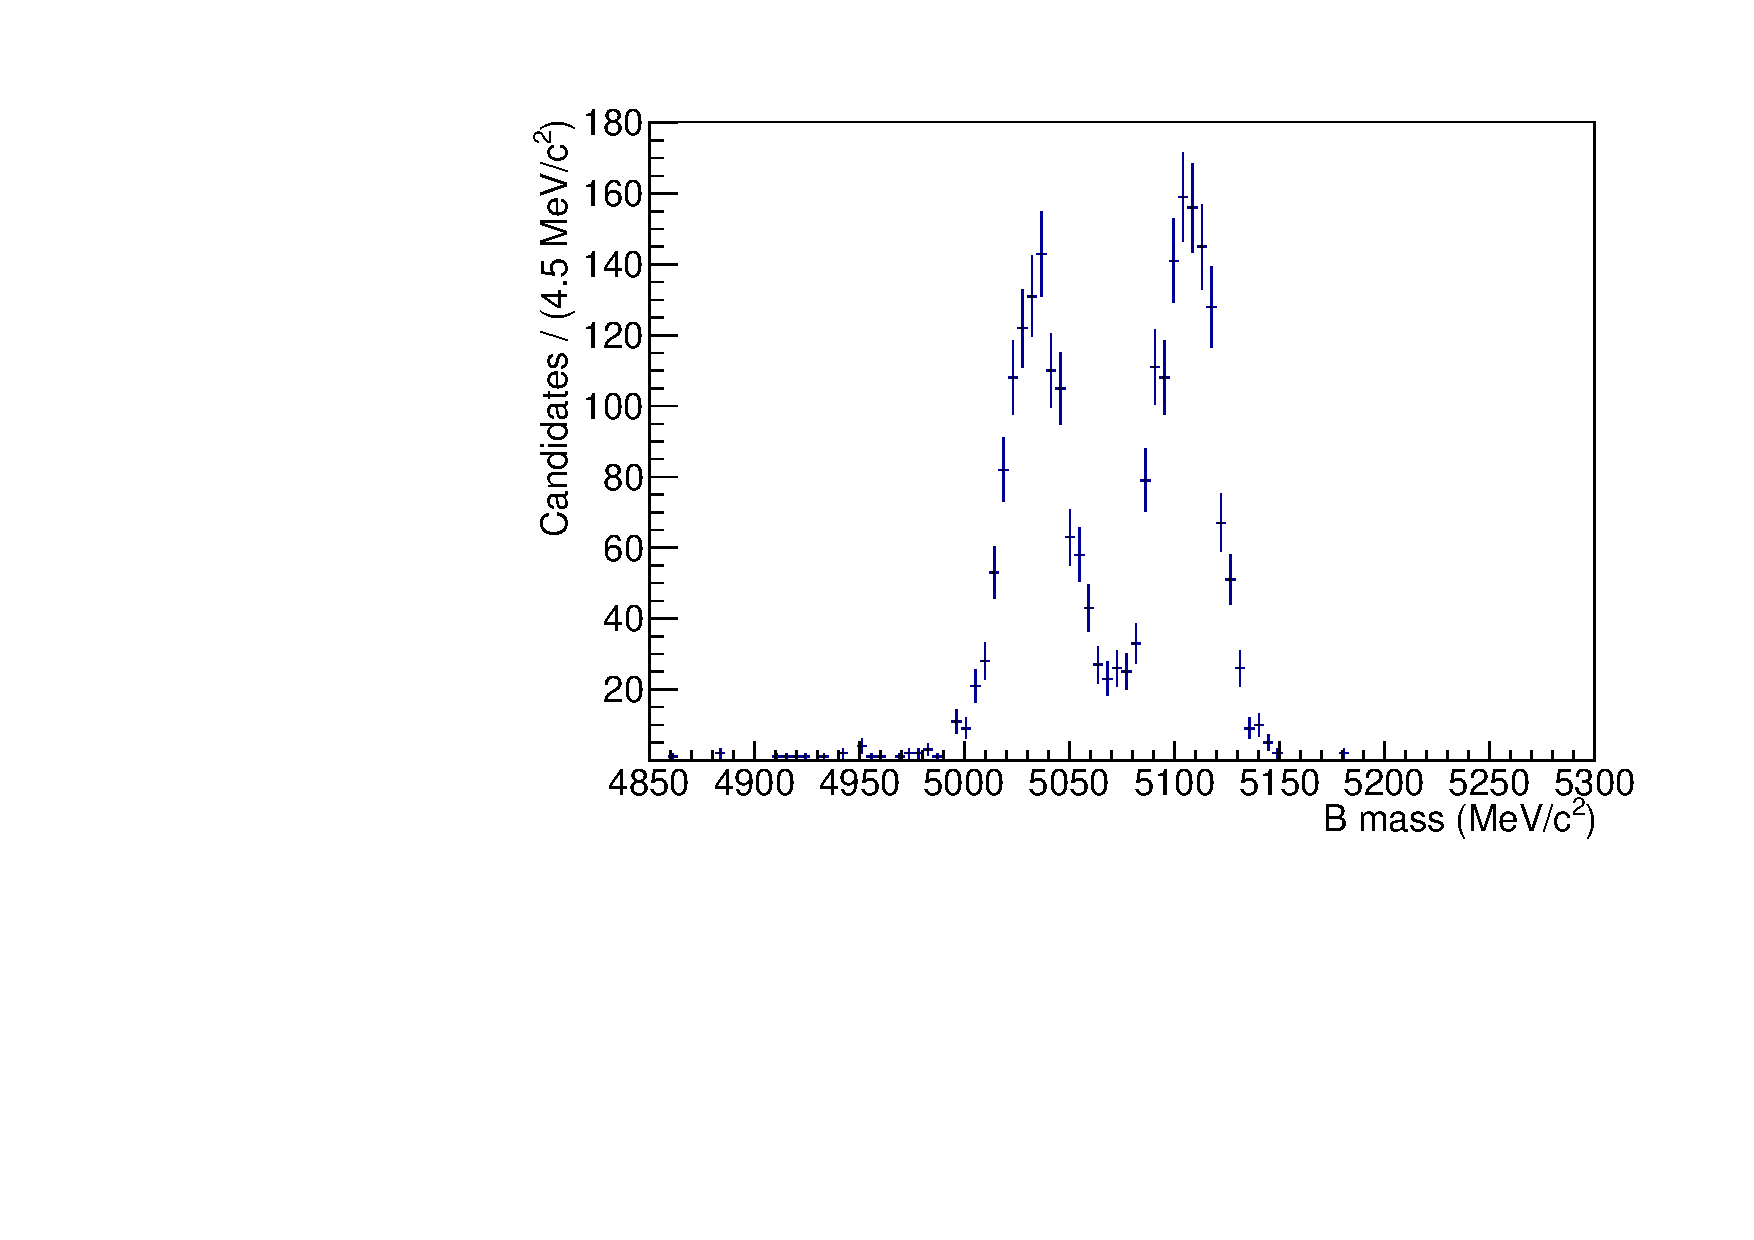
\includegraphics[width=0.5\linewidth]{figures/fitComponents/horns.pdf}
\caption{Distribution of simulated \decay{\Bm}{(\decay{\Dstarz}{\Dz\piz})\Kstarm} events, where the \piz is missed in reconstruction and the \Dstarz is in helicity state 0.}
\label{fig:horns}
\end{figure}

This distribution is modelled using the Horns function, described below. The underlying kinematic distribution is a parabola, $p_{HORNS}(x)$, with kinematics endpoints $a$ and $b$ where

\begin{align}
p_{HORNS}(x) &= \begin{cases}
\left(x - \frac{a+b}{2}\right)^2, & \text{ if $a \leq x \leq b$}\\ 	
0, & \text{ otherwise.}
\end{cases} 
\end{align}

The parabola is convolved with two Gaussians in order to account for resolution effects. Given a Gaussian function of mean $\mu$ and width $\sigma$, $G(\mu,\sigma)$, a Double Gaussian can be constructed as,

\begin{equation}
DG(x) = f_G G(x|\mu,\sigma) + \left(1-f_G\right) G(x|\mu,R_{\sigma}\sigma) \text{ , }
\end{equation}

where $\sigma$ is the width of the first Gaussian, $f_G$ is the fraction contained by the first Gaussian and $R_{\sigma}$ is the relative width between the two. Additionally, selection effects can affect the shape such that one peak is higher than the other. This is taken into account by introducing a linear polynomial with a slope of $1 - \xi$, where $0 \leq \xi \leq 1$. As $\xi \rightarrow 0$, the left hand peak decreases in size relative to the right hand peak. The resulting Horns function is,

\begin{equation}
\text{Horns}(m) = \int_a^b dx \left(x - \frac{a+b}{2}\right)^2 DG(x|m,\sigma,f_G,R_{\sigma}) \left( \frac{1 - \xi_{HORNS}}{b - a}x + \frac{b\xi_{HORNS} - a}{b - a}\right),
\label{eqn:horns}
\end{equation}

where $m$ is the mass variable to be fitted and $x$ is the integration variable in the convolution.

\subsubsection{Hill function}

Consider the \decay{\Bm}{\Dstarz\Kstarm}, \decay{\Dstarz}{\Dz\gamma}, where the \Dstarz is in helicity state 0. The helicity of the \Dstarz, the fact that the \Pgamma is spin-1 and the requirement that angular momentum is conserved mean that the \Pgamma will decay predominantly along $\theta = 90^{\circ}$ or $\theta = 270^{\circ}$. The fraction of momentum carried by the photon is the same in both of these cases, so no double peak structure is seen, giving a distribution shown in Figure \ref{fig:hill}.

\begin{figure}[h]
\centering
\includegraphics[width=0.5\linewidth]{figures/fitComponents/hill.pdf}
\caption{Distribution of simulated \decay{\Bm}{(\decay{\Dstarz}{\Dz\gamma})\Kstarm} events, where the \Pgamma is missed in reconstruction and the \Dstarz is in helicity state 0.}
\label{fig:hill}
\end{figure}

This distribution is modelled using the Hill function, described below. The underlying kinematic distribution is a parabola with negative curvature, $p_{HILL}(x)$, and kinematic endpoints $a$ and $b$ where

\begin{align}
p_{HILL}(x) &= \begin{cases}
-(x - a)(x - b), & \text{ if $a \leq x \leq b$}\\ 	
0, & \text{ otherwise.}
\end{cases} 
\end{align}

As with the Horns function, this parabola is convolved with a Double Gaussian and a linear polynomial to account for resolution and selection effects respectively. The resulting Hill function is,

\begin{equation}
\text{Hill}(m) = \int_a^b dx \left[-(x - a)(x - b)\right] DG(x|m,\sigma,f_G,R_{\sigma}) \left( \frac{1 - \xi_{HILL}}{b - a}x + \frac{b\xi_{HILL} - a}{b - a}\right),
\label{eqn:hill}
\end{equation}

where $m$ is the mass variable to be fitted and $x$ is the integration variable in the convolution.

%As the distribution of $\theta$ has a one-to-one correspondence with the reconstructed \Bm mass, a \Dstar of +1 or -1 would be indistiguishable in \Bm mass therefore these values are grouped together. 
This Hill function also applies to the \decay{\Bm}{\Dstarz\Kstarm}, \decay{\Dstarz}{\Dz\piz}, where the \Dstarz is in helicity state $\pm$1.

\subsubsection{Little Horns function}

For the configuration \decay{\Bm}{\Dstarz\Kstarm}, \decay{\Dstarz}{\Dz\gamma}, where the \Dstarz is in helicity state $\pm$1, the \Bm mass distribution is slightly different, as shown in Figure \ref{fig:littlehorns}.

\begin{figure}[h]
\centering
\includegraphics[width=0.5\linewidth]{figures/fitComponents/littlehorns.pdf}
\caption{Distribution of simulated \decay{\Bm}{(\decay{\Dstarz}{\Dz\gamma})\Kstarm} events, where the \Pgamma is missed in reconstruction and the \Dstarz is in helicity state $\pm$1.}
\label{fig:littlehorns}
\end{figure}

This is modelled using the Little Horns shape, described below. The underlying kinematic distribution is described by a parabola, $p_{LITTLEHORNS}(x)$, and kinematic endpoints $a$ and $b$ where

\begin{align}
p_{LITTLEHORNS}(x) &= \begin{cases}
\left(x - \frac{a+b}{2}\right)^2 + \left(\frac{a-b}{2}\right)^2, & \text{ if $a \leq x \leq b$}\\ 	
0, & \text{ otherwise.}
\end{cases} 
\end{align}

Again, this distribution is convolved with a Double Gaussian and linear polynomial to describe the resolution and selection effects respectively. This results in a Little Horns function

\begin{multline}
\text{LittleHorns}(m) = \int_a^b dx \biggl\{ \left[ \left( x - \frac{a+b}{2} \right) ^2 + \left( \frac{a-b}{2} \right) ^2 \right] DG(x|m,\sigma,f_G,R_{\sigma}) \\
\left( \frac{1 - \xi_{LITTLEHORNS}}{b - a}x + \frac{b\xi_{LITTLEHORNS} - a}{b - a} \right) \biggr\}
\label{eqn:littlehorns}
\end{multline}

\subsubsection{Total partially reconstructed function}

Each of these partially reconstructed shapes contribute to the mass fit in the \Bm mass region below the signal peak. Table \ref{helicityamplitudes} summarises the use of the different analytic shapes described: Horns, Hill and Little Horns functions. 

\begin{table}[h]
\centering
\resizebox{\textwidth}{!}{
\begin{tabular}{cccc}
Decay mode & Helicity of \Dstar & $\theta$ dependence & Function \\
\hline
\decay{\Bm}{(\decay{\Dstarz}{\Dz[\piz]})\Kstarm} & 0 & $\left(x - \frac{a+b}{2}\right)^2$ & Horns, from Eq.~\ref{eqn:horns} \\
\decay{\Bm}{(\decay{\Dstarz}{\Dz[\piz]})\Kstarm} & $\pm$1 & $-(x - a)(x - b)$ & Hill, from Eq.~\ref{eqn:hill} \\
\decay{\Bm}{(\decay{\Dstarz}{\Dz[\gamma]})\Kstarm} & 0 & $-(x - a)(x - b)$ & Hill, from Eq.~\ref{eqn:hill} \\
\decay{\Bm}{(\decay{\Dstarz}{\Dz[\gamma]})\Kstarm} & $\pm$1 & $\left(x - \frac{a+b}{2}\right)^2 + \left(\frac{a-b}{2}\right)^2$ & Little Horns, from Eq.~\ref{eqn:littlehorns} \\
\decay{\Bz}{(\decay{\Dstarp}{\Dz[\pip]})\Kstarm} & 0 & $\left(x - \frac{a+b}{2}\right)^2$ & Horns, from Eq.~\ref{eqn:horns} \\
\decay{\Bz}{(\decay{\Dstarp}{\Dz[\pip]})\Kstarm} & $\pm$1 & $-(x - a)(x - b)$ & Hill, from Eq.~\ref{eqn:hill} \\
\end{tabular}}
\caption{Different partially reconstructed shapes and \Dstar helicity states and how this relates to the dependence on the helicity angle and the \B mass parameterisation}
\label{helicityamplitudes}
\end{table}

In order to obtain values for the various parameters in these shapes simulated samples were generated and the full reconstruction and selection was applied. The parameters for the partially reconstructed shapes are obtained from performing individual fits to the simulated samples using the functions given by equations \ref{eqn:horns}, \ref{eqn:hill} and \ref{eqn:littlehorns}, the fits are shown in Figures \ref{partrecofitsLL} and \ref{partrecofitsDD}. All the parameters for these shapes are fixed in the mass fit from these fits to simulated distributions. Distributions in \Bm mass of \runone and \runtwo simulated events for partially reconstructed decays are considered sufficiently similar to use the same shapes for both data-taking periods.

%\begin{figure}[!h]
%\includegraphics[width=\linewidth]{figures/compareMC/run1vsrun2MC_partreco_LL.pdf}
%\includegraphics[width=\linewidth]{figures/compareMC/run1vsrun2MC_partreco_DD.pdf}
%\caption{Comparison of partially reconstructed MC between Run 1 (blue) and 2015 (red). The different shapes correspond to different \Dstar\Kstar modes, descibed in Section \ref{sec:massfit:partreco}}
%\label{parterecofits}
%\end{figure}


\begin{figure}[h]
\includegraphics[width=0.5\linewidth]{figures/fitComponents/Bupi010_LL.pdf}
\put(-170,70) {(a)}
\includegraphics[width=0.5\linewidth]{figures/fitComponents/Bupi101_LL.pdf}
\put(-170,70) {(b)}
\hfill
\includegraphics[width=0.5\linewidth]{figures/fitComponents/Bugamma010_LL.pdf}
\put(-170,70) {(c)}
\includegraphics[width=0.5\linewidth]{figures/fitComponents/Bugamma101_LL.pdf}
\put(-170,70) {(d)}
\hfill
\includegraphics[width=0.5\linewidth]{figures/fitComponents/Bdpi010_LL.pdf}
\put(-170,70) {(e)}
\includegraphics[width=0.5\linewidth]{figures/fitComponents/Bdpi101_LL.pdf}
\put(-170,70) {(f)}
\caption{Fit to $B \to D^*K^*$ \runone simulated samples in all the different modes for LL candidates (a) \decay{\Bm}{(\decay{\Dstarz}{\Dz[\piz]})\Kstarm} 0, (b) \decay{\Bm}{(\decay{\Dstarz}{\Dz[\piz]})\Kstarm} $\pm$1, (c) \decay{\Bm}{(\decay{\Dstarz}{\Dz[\gamma]})\Kstarm} 0, (d) \decay{\Bm}{(\decay{\Dstarz}{\Dz[\gamma]})\Kstarm} $\pm$1, (e) \decay{\Bd}{(\decay{\Dstarp}{\Dz[\pip]})\Kstarm} 0, and (f) \decay{\Bd}{(\decay{\Dstarp}{\Dz[\pip]})\Kstarm} $\pm$1}
\label{partrecofitsLL}
\end{figure}

\begin{figure}[h]
\includegraphics[width=0.5\linewidth]{figures/fitComponents/Bupi010_DD.pdf}
\put(-170,70) {(a)}
\includegraphics[width=0.5\linewidth]{figures/fitComponents/Bupi101_DD.pdf}
\put(-170,70) {(b)}
\hfill
\includegraphics[width=0.5\linewidth]{figures/fitComponents/Bugamma010_DD.pdf}
\put(-170,70) {(c)}
\includegraphics[width=0.5\linewidth]{figures/fitComponents/Bugamma101_DD.pdf}
\put(-170,70) {(d)}
\hfill
\includegraphics[width=0.5\linewidth]{figures/fitComponents/Bdpi010_DD.pdf}
\put(-170,70) {(e)}
\includegraphics[width=0.5\linewidth]{figures/fitComponents/Bdpi101_DD.pdf}
\put(-170,70) {(f)}
\caption{Fit to $B \to D^*K^*$ \runone simulated samples in all the different modes for DD candidates (a) \decay{\Bm}{(\decay{\Dstarz}{\Dz[\piz]})\Kstarm} 0, (b) \decay{\Bm}{(\decay{\Dstarz}{\Dz[\piz]})\Kstarm} $\pm$1, (c) \decay{\Bm}{(\decay{\Dstarz}{\Dz[\gamma]})\Kstarm} 0, (d) \decay{\Bm}{(\decay{\Dstarz}{\Dz[\gamma]})\Kstarm} $\pm$1, (e) \decay{\Bd}{(\decay{\Dstarp}{\Dz[\pip]})\Kstarm} 0, and (f) \decay{\Bd}{(\decay{\Dstarp}{\Dz[\pip]})\Kstarm} $\pm$1}
\label{partrecofitsDD}
\end{figure}

These partially reconstructed decays contribute six shapes in the same region of the \Bm mass fit at a lower invariant mass compared to the signal, from 4900 - 5230 MeV. The shape parameters are all fixed in the mass fit, however, each of the shapes also has an associated yield. As the shapes all occur in the same region of \Bm mass, allowing the six individual yields to vary leads to an unstable fit. Therefore, it is necessary to apply additional constraints, in the form of fixing ratios of different yields in order to have a stable fit. 

The total partially reconstructed PDF is given by,
\begin{equation}
P_{partreco} = f_0P_0 + (1 - f_0)P_{\pm 1}
\label{partrecofunction}
\end{equation}
where $P_0$ and $P_{\pm 1}$, which represent the total PDF for the \Dstar helicity states 0 and $\pm$1 respectively, are given by
\begin{align*}
P_0 &= P^{Bu,\pi}_0 + c^{Bu,\gamma}_0P^{Bu,\gamma}_0 + c^{Bd,\pi}_0P^{Bd,\pi}_0 \\
P_{\pm 1} &= P^{Bu,\pi}_{\pm 1} + c^{Bu,\gamma}_{\pm 1}P^{Bu,\gamma}_{\pm 1} + c^{Bd,\pi}_{\pm 1}P^{Bd,\pi}_{\pm 1} \text{ .}
\end{align*}
The yield ratios between \decay{\Bm}{(\decay{\Dstarz}{\Dz[\piz]})\Kstarm}, \decay{\Bm}{(\decay{\Dstarz}{\Dz[\gamma]})\Kstarm} and \decay{\Bd}{(\decay{\Dstarp}{\Dz[\pip]})\Kstarm} are fixed separately for the 0 and $\pm$1 helicity states of the \Dstar. The expected yield ratios, $c^{Bu,\gamma}_0$, $c^{Bd,\pi}_0$, $c^{Bu,\gamma}_{\pm 1}$ and $c^{Bd,\pi}_{\pm 1}$, can be individually calculated from knowledge of the ratio of production of the relevant decays and the ratio of the efficiencies of the relevant decays passing the selection, detailed in Section \ref{sec:selection}, for example, 

\begin{align}
c^{Bu,\gamma}_0 &= \frac{N(\decay{\Bm}{(\decay{\Dstarz}{\Dz\gamma})\Kstarm}\ 0)}{N(\decay{\Bm}{(\decay{\Dstarz}{\Dz\piz})\Kstarm}\ 0)} \nonumber \\ 
&= \frac{\mathcal{B}(\decay{\Bm}{(\decay{\Dstarz}{\Dz\gamma})\Kstarm}\ 0)}{\mathcal{B}(\decay{\Bm}{(\decay{\Dstarz}{\Dz\piz})\Kstarm}\ 0)} \times \frac{\epsilon_{sel}(\decay{\Bm}{(\decay{\Dstarz}{\Dz\gamma})\Kstarm}\ 0)}{\epsilon_{sel}(\decay{\Bm}{(\decay{\Dstarz}{\Dz\piz})\Kstarm}\ 0)}
\label{partrecoexample}
\end{align}

where $N$ represents the yield, $\mathcal{B}$ represents the branching fraction and $\epsilon_{sel}$ represents the selection efficiency of the partially reconstructed decay. The ratio of branching fractions is used to estimate the expected ratio of production in the collision of the two partially reconstructed decays being considered, these branching fractions are given in Table \ref{partrecoBRs}. The selection efficiency, $\epsilon_{sel}$, calculated using simulated partially reconstructed samples, is defined as the number of simulated events passing the selection compared to the number of simulated events generated. This gives ratio of the probability of the two partially reconstructed decays under consideration passing the selection. Using Equation \ref{partrecoexample} and equivalent calculations for the other yield ratios, the estimated yield ratios given in Table \ref{fixedyieldratios}; these values are fixed in the mass fit. 

\begin{table}[h]
\centering
\begin{tabular}{c|c}
Mode & Branching ratio \\
\hline
\decay{\Bm}{(\decay{\Dstarz}{\Dz\piz})\Kstarm} & $(5.0 \pm 0.9) \times 10^{-4}$ \\
\decay{\Bm}{(\decay{\Dstarz}{\Dz\gamma})\Kstarm} & $(3.1 \pm 0.6) \times 10^{-4}$ \\
\decay{\Bd}{(\decay{\Dstarp}{\Dz\pip})\Kstarm} & $(2.2 \pm 0.4) \times 10^{-4}$ \\
\end{tabular}
\caption{Branching ratios for the different partially reconstructed decay modes~\cite{PDG2014}}
\label{partrecoBRs}
\end{table}

\begin{table}[h]
\centering
\begin{tabular}{ccc}
\hline
& LL & DD \\
\hline
$c^{Bu,\gamma}_0$ & $0.53 \pm 0.14$ & $0.51 \pm 0.14$ \\[3mm]
$c^{Bd,\pi}_0$ & $0.38 \pm 0.14$ & $0.37 \pm 0.14$ \\[3mm]
$c^{Bu,\gamma}_{\pm 1}$ & $0.53 \pm 0.14$ & $0.51 \pm 0.14$ \\[3mm]
$c^{Bd,\pi}_{\pm 1}$ & $0.38 \pm 0.14$ & $0.38 \pm 0.14$ \\[3mm]
\hline
\end{tabular}
\caption{Yield ratios fixed in the mass fit for the partially reconstructed backgrounds}
\label{fixedyieldratios}
\end{table}

Other backgrounds investigated in this analysis, but not included in the mass fit are discussed in Section \ref{sec:backgrounds}.


\subsection{Mass fit to the data in the favoured modes}
\label{sec:massfit:fit}

A fit to the invariant B mass in the \kpi and \kpipipi favoured mode is performed using the shapes discussed in Sections \ref{sec:massfit:signal}, \ref{sec:massfit:combinatorial} and \ref{sec:massfit:partreco}. The total PDF is given by
\begin{equation}
P_{tot} = N_{sig}P_{sig} + N_{comb}P_{comb} + N_{dstkst}P_{dstkst} \text{ ,}
\end{equation}
where $N_{sig}$, $N_{comb}$ and $N_{dstkst}$ are the yields of the signal, combinatorial and partially reconstructed yields respectively. The signal PDF, $P_{sig}$, is given by Equation~\ref{DCBshape}, the partially reconstructed PDF, $P_{dstkst}$, is given by Equation~\ref{partrecofunction} and the combinatorial PDF is an exponential, $P_{comb} = e^{\beta m}$, where the slope parameter $\beta$ is able to vary in the fit. The yield of the signal and combinatorial shape, $N_{sig}$ and $N_{comb}$, are left to vary without constraint, as well as the peak position, $\mu$, and width, $\sigma$, of the signal PDF. The only parameters able to vary in the partially reconstructed background are the yield ratio between the 0 and $\pm$1 amplitudes, $f_0$, and the overall yield, $N_{dstkst}$.

Figures \ref{massfitskpi} and \ref{massfitsk3pi} show the fits to the invariant B mass distribution in the \kpi and \kpipipi favoured mode respectively for LL and DD candidates in both Run 1 and Run 2. The estimated signal yields extracted from these fits are given in Table \ref{signalyields}. The full fit results for the \kpi and \kpipipi fits are shown in Tables \ref{fitresultskpi} and \ref{fitresultsk3pi} respectively.

\begin{table}
\centering
\begin{tabular}{l|cc|cc}
\hline
& \multicolumn{2}{c}{\kpi} & \multicolumn{2}{c}{\kpipipi} \\
& \runone & \runtwo & \runone & \runtwo \\
\hline
LL & $220 \pm 16$ & $388 \pm 21$ & $87 \pm 10$ & $215 \pm 15$ \\
DD & $505 \pm 24$ & $901 \pm 33$ & $205 \pm 16$ & $516 \pm 25$ \\
\hline
\end{tabular}
\caption{Signal yields from the \kpi and \kpipipi mass fits for both \KS reconstruction types and data-taking periods separately.}
\label{signalyields}
\end{table}

\begin{figure}
\centering
\includegraphics[width=0.8\linewidth]{figures/fitComponents/massFit_LL_KPi_run1.pdf}
\put(-280,120) {(a)}
\hfill
\includegraphics[width=0.8\linewidth]{figures/fitComponents/massFit_DD_KPi_run1.pdf}
\put(-280,120) {(b)}
\hfill
\includegraphics[width=0.8\linewidth]{figures/fitComponents/massFit_LL_KPi_run2.pdf}
\put(-280,120) {(c)}
\hfill
\includegraphics[width=0.8\linewidth]{figures/fitComponents/massFit_DD_KPi_run2.pdf}
\put(-280,120) {(d)}
\caption{Fits to the \kpi invariant B mass distribution for (a) \runone LL, (b) \runone DD, (c) \runtwo LL, and (d) \runtwo DD.}
\label{massfitskpi}
\end{figure}

\begin{figure}
\centering
\includegraphics[width=0.8\linewidth]{figures/fitComponents/massFit_LL_KPiPiPi_run1.pdf}
\put(-280,120) {(a)}
\hfill
\includegraphics[width=0.8\linewidth]{figures/fitComponents/massFit_DD_KPiPiPi_run1.pdf}
\put(-280,120) {(b)}
\hfill
\includegraphics[width=0.8\linewidth]{figures/fitComponents/massFit_LL_KPiPiPi_run2.pdf}
\put(-280,120) {(c)}
\hfill
\includegraphics[width=0.8\linewidth]{figures/fitComponents/massFit_DD_KPiPiPi_run2.pdf}
\put(-280,120) {(d)}
\caption{Fits to the \kpipipi invariant B mass distribution for (a) \runone LL, (b) \runone DD, (c) \runtwo LL, and (d) \runtwo DD.}
\label{massfitsk3pi}
\end{figure}

\begin{table}[h]
\centering
\resizebox{\textwidth}{!}{
\begin{tabular}{l|cc|cc}
\hline
& \multicolumn{2}{c}{Run 1} & \multicolumn{2}{c}{Run 2} \\
& LL & DD & LL & DD \\
\hline
$\beta$ & $(-4.8 \pm 0.5) \times 10^{-3}$ & $(-2.8 \pm 0.3) \times 10^{-3}$ & $(-4.4 \pm 0.5) \times 10^{-3}$ & $(-2.5 \pm 0.2) \times 10^{-3}$ \\
$f_0$ & $0.15 \pm 0.08$ & $0.12 \pm 0.05$ & $0.18 \pm 0.05$ & $0.06 \pm 0.04$ \\
$\mu$ & $5280.7 \pm 0.8$ & $5280.7 \pm 0.6$ & $5278.5 \pm 0.8$ & $5278.6 \pm 0.5$ \\
$N_{comb}$ & $167 \pm 20$ & $472 \pm 34$ & $223 \pm 24$ & $1100 \pm 50$ \\
$N_{dstkst}$ & $338 \pm 23$ & $810 \pm 36$ & $654 \pm 31$ & $1397 \pm 49$ \\
$N_{sig}$ & $220 \pm 16$ & $505 \pm 24$ & $388 \pm 21$ & $901 \pm 33$ \\
$\sigma$ & $10.2 \pm 0.7$ & $11.5 \pm 0.5$ & $12.2 \pm 0.6$ & $11.5 \pm 0.4$ \\
\hline
\end{tabular}}
\caption{Fit results from the \kpi favoured mode for LL and DD candidates, corresponding to the fits in Figure \ref{massfitskpi}. The parameter $\beta$ is the combinatorial background slope, $f_0$ is the yield ratio between 0 and $\pm$1 helicity amplitudes, $\sigma$ is the floating width of the signal shape, and $N_{sig}$, $N_{comb}$ and $N_{dstkst}$ are the yields of signal, combinatorial background and partially reconstructed decays respectively}
\label{fitresultskpi}
\end{table}

\begin{table}[h]
\centering
\resizebox{\textwidth}{!}{
\begin{tabular}{l|cc|cc}
\hline
& \multicolumn{2}{c}{Run 1} & \multicolumn{2}{c}{Run 2} \\
& LL & DD & LL & DD \\
\hline
$\beta$ & $(-5.2 \pm 1.1) \times 10^{-3}$ & $(-2.3 \pm 0.4) \times 10^{-3}$ & $(-4.4 \pm 0.5) \times 10^{-3}$ & $(-2.1 \pm 0.2) \times 10^{-3}$ \\
$f_0$ & $0.26 \pm 0.11$ & $0.20 \pm 0.08$ & $0.15 \pm 0.07$ & $0.16 \pm 0.05$ \\
$\mu$ & $5281.3 \pm 1.3$ & $5283.9 \pm 0.9$ & $5278.7 \pm 1.0$ & $5277.7 \pm 0.7$ \\
$N_{comb}$ & $50 \pm 12$ & $252 \pm 24$ & $168 \pm 20$ & $707 \pm 40$ \\
$N_{dstkst}$ & $154 \pm 15$ & $317 \pm 24$ & $342 \pm 23$ & $914 \pm 40$ \\
$N_{sig}$ & $102 \pm 10$ & $226 \pm 16$ & $244 \pm 16$ & $578 \pm 27$ \\
$\sigma$ & $11.4 \pm 1.0$ & $11.3 \pm 0.8$ & $12.9 \pm 0.8$ & $13.1 \pm 0.6$ \\
\hline
\end{tabular}}
\caption{Fit results from the \kpipipi favoured mode for LL and DD candidates, corresponding to the fits in Figure \ref{massfitsk3pi}. The parameter $\beta$ is the combinatorial background slope, $f_0$ is the yield ratio between 0 and $\pm$1 helicity amplitudes, $\sigma$ is the floating width of the signal shape, and $N_{sig}$, $N_{comb}$ and $N_{dstkst}$ are the yields of signal, combinatorial background and partially reconstructed decays respectively}
\label{fitresultsk3pi}
\end{table}


\clearpage

\clearpage
\begin{savequote}[8cm]
\textlatin{Neque porro quisquam est qui dolorem ipsum quia dolor sit amet, consectetur, adipisci velit...}

There is no one who loves pain itself, who seeks after it and wants to have it, simply because it is pain...
  \qauthor{--- Cicero's \textit{de Finibus Bonorum et Malorum}}
\end{savequote}

\chapter{\label{ch:5-cpfit}Fits for \CP observables in two- and four-body decays} 

\minitoc

In this section the \CP observables are measured using the yields of \btodkst in each \D decay mode for both \Bp and \Bm decays.

The setup of the \CP fit is outlined in Section \ref{sec:cpfit:setup}, followed by the fit results in Section \ref{sec:cpfit:results}. Section \ref{sec:systematics} outlines the systematic uncertainties and the results of the \CP observables are summarised in Section \ref{sec:cpfit:summary}.

\section{Setup of \CP fit}
\label{sec:cpfit:setup}

The fit to data is performed on the invariant mass of B candidates. A simultaneous fit stategy is employed to fit each of the D decay modes as well as two bins of B charge ($B^+$ and $B^-$), two bins of $K_s$ track type (LL and DD) and two bins of data type (Run 1 and Run 2), resulting in 56 bins in total.

As discussed in Section \ref{sec:massfit:range} the \CP fit is performed from 5230 MeV. The components and shapes of the \CP fit are the same as those described in Section \ref{sec:massfit}. The mean and width of the signal shape are shared across the different run periods and across modes of the same number of final state particles, but the mean and width are allowed to be different for the 2 and 4-body modes. The shape and yield of the partially reconstructed background is completely fixed, with separate values for LL and DD candidates. The shape is fixed as described in Section \ref{sec:massfit:partreco}, using the yield ratios given in Table \ref{fixedyieldratios}. The total yield is fixed from the fits in Figures \ref{massfitskpi} and \ref{massfitsk3pi}, the values for the total partially reconstructed yield in each of the simultaneous fit categories is given in Appendix \ref{sec:app:partrecoyields}. The shape of the combinatoric background is shared across all modes of the same number of final state particles, but has different values for LL and DD candidates, as well as two and four-body D modes.

The \CP fit parameters are the \CP observables \Akpi, \Akk, \Apipi, \Rkk, \Rpipi, \Rptwo, \Rmtwo, \Akpipipi, \Apipipipi, \Rpipipipi, \Rpfour and \Rmfour, which relate to the physics parameters of interest as shown in Equations \ref{exp_Acp} - \ref{exp_R4pi}.

\subsection{Corrections to yield ratios}
\label{sec:cpfit:efficiencies}

The \CP fit measures seven \CP observables, \Rkk, \Rpipi, \Rptwo, \Rmtwo, \Rpipipipi, \Rpfour and \Rmfour, which relate to the yield ratios with respect to \decay{\Bm}{\D(\Km\pip)\Kstarm} and \decay{\Bm}{\D(\Km\pip\pim\pip)\Kstarm} for two- and four-bosy observables respectively. In order to extract these \CP observables from the raw yield ratios, various efficiency corrections, taken from simulated signal samples, must be applied.

For the GLW modes, the fit takes the raw value of the yield ratio and applies efficiency corrections to extract \Rkk, \Rpipi and \Rpipipipi as shown in Equation \ref{effcorrectionglw2body} and \ref{effcorrectionglw4body}, where $\epsilon_{sel}$ and $\epsilon_{pid}$ are the selection and PID efficiencies respectively. The values for these selection and PID efficiency corrections are given in Tables \ref{seleff} and \ref{pideff} respectively.

{\footnotesize
\begin{equation}
R_{hh} = \frac{N(\decay{\Bm}{\D(h^+h^-)\Kstarm})}{N(\decay{\Bm}{\D(\Km\pip)\Kstarm})} \times \frac{\BR(\decay{\Dz}{\Km\pip})}{\BR(\decay{\Dz}{hh})} \times \frac{\epsilon_{\text{sel}}(K\pi)}{\epsilon_{\text{sel}}(hh)} \times \frac{\epsilon_{\text{pid}}(K\pi)}{\epsilon_{\text{pid}}(hh)}
\label{effcorrectionglw2body}
\end{equation}

\begin{equation}
R_{\pi\pi\pi\pi} = \frac{N(\decay{\Bm}{\D(\pip\pim\pip\pim)\Kstarm})}{N(\decay{\Bm}{\D(\Km\pip\pim\pip)\Kstarm})} \times \frac{\BR(\decay{\Dz}{\Km\pip\pim\pip})}{\BR(\decay{\Dz}{\pi\pi\pi\pi})} \times \frac{\epsilon_{\text{sel}}(K\pi\pi\pi)}{\epsilon_{\text{sel}}(\pi\pi\pi\pi)} \times \frac{\epsilon_{\text{pid}}(K\pi\pi\pi)}{\epsilon_{\text{pid}}(\pi\pi\pi\pi)} 
\label{effcorrectionglw4body}
\end{equation}}

As the final state in the ADS mode is almost identical to the charge favoured, the selection efficiencies that are common to both are assumed to cancel. There are only two differences between the selection for the ADS mode and the charge favoured mode; the tighter BDT selection for DD candidates and the double misID veto, which is only applied to the ADS mode. Equations \ref{effcorrectionads2body} and \ref{effcorrectionads4body} describe the effciency corrections required to extract \Rptwo, \Rmtwo, \Rpfour and \Rmfour from the raw yield ratios, where $\epsilon_{bdt}$ and $\epsilon_{veto}$ are the BDT and veto efficiencies respectively. The values for these BDT and veto efficiency corrections are given in Tables \ref{bdteff} and \ref{vetoeff} respectively.

{\footnotesize
\begin{equation}
R^{\pm}_{K\pi} = \frac{N(\decay{\Bpm}{\D(\Kmp\pipm)\Kstarpm})}{N(\decay{\Bpm}{\D(\Kpm\pimp)\Kstarpm})} \times \frac{\epsilon_{\text{bdt}}(K\pi)}{\epsilon_{\text{bdt}}(\pi K)} \times \frac{1}{\epsilon_{\text{veto}}(\pi K)}
\label{effcorrectionads2body}
\end{equation}

\begin{equation}
R^{\pm}_{K\pi\pi\pi} = \frac{N(\decay{\Bpm}{\D(\Kmp\pipm\pimp\pipm)\Kstarpm})}{N(\decay{\Bpm}{\D(\Kpm\pimp\pipm\pimp)\Kstarpm})} \times \frac{\epsilon_{\text{bdt}}(K\pi\pi\pi)}{\epsilon_{\text{bdt}}(\pi K\pi\pi)} \times \frac{1}{\epsilon_{\text{veto}}(\pi K\pi\pi)}
\label{effcorrectionads4body}
\end{equation}}

All the efficiency corrections that are used as inputs to the fit are summarised in Table \ref{fitinputs}. The final fit to the data measures $A_{K\pi}$, $A_{KK}$, $A_{\pi\pi}$, $R_{KK}$, $R_{\pi\pi}$, $R^+$,  $R^-$, $A_{K\pi\pi\pi}$, $A_{\pi\pi\pi\pi}$, $R_{\pi\pi\pi\pi}$, $R^+_{K3\pi}$ and  $R^-_{K3\pi}$, which all have the relevant efficiency corrections applied.


\subsubsection{Signal efficiencies from simulation}
\label{sec:cpfit:efficiencies:signal}

The signal efficiency of the stripping, trigger and offline selection, $\epsilon_{sel}$, is extracted from samples of simulated signal events in order to be used in Equations \ref{effcorrectionglw2body} and \ref{effcorrectionglw4body}. These values have been calculated separately for \runone and \runtwo samples as well as LL and DD categories, as shown in Table \ref{seleff}. It can be seen that the LL selection efficiency drops in \runtwo, this is thought to be due to the \KS momentum being slightly higher in \runtwo giving fewer \KS mesons decay within the \velo. PID efficiencies have not been included in these calculations; they are extracted from the {\tt PIDCalib} package~\cite{PIDCalib} and are detailed in Section \ref{sec:cpfit:efficiencies:pid}.

\begin{table}[h]
\centering
\begin{tabular}{c|cc|cc}
\hline
& \multicolumn{2}{c}{Run 1} & \multicolumn{2}{c}{Run 2} \\
& LL & DD & LL & DD \\
\hline
$\epsilon_{sel}(K\pi)$ & $0.0939 \pm 0.0011$ & $0.2519 \pm 0.0018$ & $0.1266 \pm 0.0011$ & $0.3155 \pm 0.0017$ \\
$\epsilon_{sel}(KK)$ & $0.0919 \pm 0.0011$ & $0.2450 \pm 0.0018$ & $0.1189 \pm 0.0010$ & $0.2923 \pm 0.0016$ \\
$\epsilon_{sel}(\pi\pi)$ & $0.1015 \pm 0.0012$ & $0.2584 \pm 0.0018$ & $0.1292 \pm 0.0011$ & $0.3309 \pm 0.0017$ \\
$\epsilon_{sel}(K\pi\pi\pi)$ & $0.0288 \pm 0.0006$ & $0.0816 \pm 0.0020$ & $0.0484 \pm 0.0004$ & $0.1229 \pm 0.0007$ \\
$\epsilon_{sel}(\pi\pi\pi\pi)$ & $0.0272 \pm 0.0013$ & $0.0825 \pm 0.0022$ & $0.0436 \pm 0.0011$ & $0.1185 \pm 0.0017$ \\
\hline
\end{tabular}
\caption{Summary of the selection efficiencies used in the \CP fit}
\label{seleff}
\end{table}

The BDT efficiency for the two- and four-body ADS modes is required for Equations \ref{effcorrectionads2body} and \ref{effcorrectionads4body}, which is obtained from samples of simulated signal events. The results are given in Table \ref{bdteff}.

\begin{table}[h]
\centering
\begin{tabular}{c|cc|cc}
\hline
& \multicolumn{2}{c}{Run 1} & \multicolumn{2}{c}{Run 2} \\
& LL & DD & LL & DD \\
\hline
$\epsilon_{bdt}(K\pi)$ & $0.947 \pm 0.005$ & $0.896 \pm 0.004$ & $0.949 \pm 0.003$ & $0.907 \pm 0.002$ \\
$\epsilon_{bdt}(\pi K)$ & $0.947 \pm 0.005$ & $0.802 \pm 0.005$ & $0.949 \pm 0.003$ & $0.826 \pm 0.003$ \\
$\epsilon_{bdt}(K\pi\pi\pi)$ & $0.938 \pm 0.010$ & $0.903 \pm 0.007$ & $0.952 \pm 0.003$ & $0.928 \pm 0.002$ \\
$\epsilon_{bdt}(\pi K\pi\pi)$ & $0.938 \pm 0.010$ & $0.838 \pm 0.009$ & $0.952 \pm 0.003$ & $0.870 \pm 0.003$ \\
\hline
\end{tabular}
\caption{Summary of the BDT efficiencies used in the \CP fit}
\label{bdteff}
\end{table}


\subsubsection{PID efficiencies}
\label{sec:cpfit:efficiencies:pid}

In this analysis the selection for the various D decays modes \decay{\D}{\kaon\pi, \kaon\kaon, \pi\pi, \pi\kaon} is almost identical apart for the particle identification requirements. Therefore it is very important to apply an efficient PID selection.

As described in Section \ref{sec:selection:pid}, the PID requirements are $DLLK < 4$ for the pion from the \Kstarm and $DLLK > 2$ and $DLLK < -2$ for the \D daughters when applied to kaons and pions respectively. The efficiencies for the various selection are determined using the {\tt PIDCalib} package~\cite{PIDCalib}. The uncertainties in the PID efficiencies are systematic and come from:

%LHCb-PROC-2011-008 ; CERN-LHCb-PROC-2011-008

\begin{itemize}
\item The use of finite samples of \Dstar calibration tracks
\item The use of finite signal track samples
\item The {\tt PIDCalib} procedure
\end{itemize}

The PID efficiencies are calculated individually for each year of data-taking and each magnet polarity. They are combined separately for \runone and \runtwo according to the efficiency corrected yields in each of the samples, to be used in the \CP fit as described in Equations \ref{effcorrectionglw2body} and \ref{effcorrectionglw4body}. The results of the PID efficienies are given in Table \ref{pideff}.

\begin{table}[h]
\centering
\begin{tabular}{c|cc|cc}
\hline
& \multicolumn{2}{c}{Run 1} & \multicolumn{2}{c}{Run 2} \\
& LL & DD & LL & DD \\
\hline
$\epsilon_{pid}(K\pi)$ & $0.734 \pm 0.002$ & $0.747 \pm 0.002$ & $0.811 \pm 0.002$ & $0.821 \pm 0.002$ \\
$\epsilon_{pid}(KK)$ & $0.812 \pm 0.002$ & $0.825 \pm 0.002$ & $0.844 \pm 0.002$ & $0.853 \pm 0.002$ \\
$\epsilon_{pid}(\pi\pi)$ & $0.670 \pm 0.002$ & $0.676 \pm 0.002$ & $0.779 \pm 0.002$ & $0.790 \pm 0.002$ \\
$\epsilon_{pid}(K\pi\pi\pi)$ & $0.630 \pm 0.002$ & $0.636 \pm 0.002$ & $0.784 \pm 0.002$ & $0.798 \pm 0.002$ \\
$\epsilon_{pid}(\pi\pi\pi\pi)$ & $0.675 \pm 0.002$ & $0.687 \pm 0.002$ & $0.822 \pm 0.002$ & $0.835 \pm 0.002$ \\
\hline
\end{tabular}
\caption{Summary of the PID efficiencies used in the \CP fit}
\label{pideff}
\end{table}

Another input to the fit is the efficiency of the double misID veto, which is required as a correction to the ADS observables, as in Equations \ref{effcorrectionads2body} and \ref{effcorrectionads4body}. Veto efficiencies calculated from data are used in the \CP fit for both two- and four-body modes, given in Table \ref{vetoeff}.

\begin{table}[h]
\centering
\begin{tabular}{c|cc|cc}
\hline
& \multicolumn{2}{c}{Run 1} & \multicolumn{2}{c}{Run 2} \\
& LL & DD & LL & DD \\
\hline
$\epsilon_{veto}(\pi K)$ & $0.905 \pm 0.009$ & $0.919 \pm 0.005$ & $0.915 \pm 0.007$ & $0.917 \pm 0.004$ \\
$\epsilon_{veto}(\pi K \pi\pi)$ & $0.895 \pm 0.005$ & $0.882 \pm 0.003$ & $0.916 \pm 0.003$ & $0.906 \pm 0.002$ \\
\hline
\end{tabular}
\caption{Summary of the veto efficiencies used in the \CP fit}
\label{vetoeff}
\end{table}

It can be seen from Table \ref{pideff} that the PID efficiency in \runtwo is higher than \runone for the PID selection used in this analysis. In order to check that the PID selection for \runone is suitable to be applied to \runtwo the misID efficiency (efficiency of a $K\pi$ candidate passing the $\pi K$ PID selection) was investigated. For the two-body mode, both the PID efficiency and misID efficiency is improved in \runtwo compared to \runone so the same PID selection can be applied to both datasets. For the four-body mode the misID efficiency is slightly worse in \runtwo compared to \runone. A low misID rate is required to reduce the crossfeed background discussed in Section \ref{sec:backgrounds:crossfeed}, which reports a negligible level of this crossfeed background in both \runone and \runtwo, therefore the misID rate is already sufficiently low and so the PID selection does not need to be tightened for \runtwo.

\subsubsection{Summary of efficiency corrections}
\label{sec:cpfit:efficiencies:summary}

The \CP fit uses signal efficiencies, BDT efficiencies, PID efficiencies and double misID veto efficiencies from simulation, as well as branching ratios from Ref~\cite{PDG2016}. Table \ref{fitinputs} summarises the values used in the \CP fit. 

\begin{table}[h]
\centering
\begin{tabular}{c|cc|cc}
\hline
& \multicolumn{2}{c}{Run 1} & \multicolumn{2}{c}{Run 2} \\
& LL & DD & LL & DD \\
\hline
$BF(\decay{\Dz}{\Km\pip})$ & \multicolumn{4}{c}{$0.0393 \pm 0.0004$} \\
$BF(\decay{\Dz}{\Kp\Km})$ & \multicolumn{4}{c}{$0.00401 \pm 0.00007$} \\
$BF(\decay{\Dz}{\pip\pim})$ & \multicolumn{4}{c}{$0.001421 \pm 0.000025$} \\
$\epsilon_{sel}(K\pi)$ & $0.0939 \pm 0.0011$ & $0.2519 \pm 0.0018$ & $0.1266 \pm 0.0011$ & $0.3155 \pm 0.0017$ \\
$\epsilon_{sel}(KK)$ & $0.0919 \pm 0.0011$ & $0.2450 \pm 0.0018$ & $0.1189 \pm 0.0010$ & $0.2923 \pm 0.0016$ \\
$\epsilon_{sel}(\pi\pi)$ & $0.1015 \pm 0.0012$ & $0.2584 \pm 0.0018$ & $0.1292 \pm 0.0011$ & $0.3309 \pm 0.0017$ \\
$\epsilon_{pid}(K\pi)$ & $0.734 \pm 0.002$ & $0.747 \pm 0.002$ & $0.811 \pm 0.002$ & $0.821 \pm 0.002$ \\
$\epsilon_{pid}(KK)$ & $0.812 \pm 0.002$ & $0.825 \pm 0.002$ & $0.844 \pm 0.002$ & $0.853 \pm 0.002$ \\
$\epsilon_{pid}(\pi\pi)$ & $0.670 \pm 0.002$ & $0.676 \pm 0.002$ & $0.779 \pm 0.002$ & $0.790 \pm 0.002$ \\
$\epsilon_{bdt}(K\pi)$ & $0.947 \pm 0.005$ & $0.896 \pm 0.004$ & $0.949 \pm 0.003$ & $0.907 \pm 0.002$ \\
$\epsilon_{bdt}(\pi K)$ & $0.947 \pm 0.005$ & $0.802 \pm 0.005$ & $0.949 \pm 0.003$ & $0.826 \pm 0.003$ \\
$\epsilon_{veto}(\pi K)$ & $0.905 \pm 0.009$ & $0.919 \pm 0.005$ & $0.915 \pm 0.007$ & $0.917 \pm 0.004$ \\
$\epsilon_{sel}(K\pi\pi\pi)$ & $0.0288 \pm 0.0006$ & $0.0816 \pm 0.0020$ & $0.0484 \pm 0.0004$ & $0.1229 \pm 0.0007$ \\
$\epsilon_{sel}(\pi\pi\pi\pi)$ & $0.0272 \pm 0.0013$ & $0.0825 \pm 0.0022$ & $0.0436 \pm 0.0011$ & $0.1185 \pm 0.0017$ \\
$\epsilon_{pid}(K\pi\pi\pi)$ & $0.630 \pm 0.002$ & $0.636 \pm 0.002$ & $0.784 \pm 0.002$ & $0.798 \pm 0.002$ \\
$\epsilon_{pid}(\pi\pi\pi\pi)$ & $0.675 \pm 0.002$ & $0.687 \pm 0.002$ & $0.822 \pm 0.002$ & $0.835 \pm 0.002$ \\
$\epsilon_{bdt}(K\pi\pi\pi)$ & $0.938 \pm 0.010$ & $0.903 \pm 0.007$ & $0.952 \pm 0.003$ & $0.928 \pm 0.002$ \\
$\epsilon_{bdt}(\pi K\pi\pi)$ & $0.938 \pm 0.010$ & $0.838 \pm 0.009$ & $0.952 \pm 0.003$ & $0.870 \pm 0.003$ \\
$\epsilon_{veto}(\pi K \pi\pi)$ & $0.895 \pm 0.005$ & $0.882 \pm 0.003$ & $0.916 \pm 0.003$ & $0.906 \pm 0.002$ \\
\hline
\end{tabular}
\caption{Table of branching fractions and efficiencies used in the \CP fit. Branching ratios are taken from the PDG~\cite{PDG2016}. All these values are fixed inputs and systematics are assigned based on the uncertainties, as detailed in Section \ref{sec:systematics}.}
\label{fitinputs}
\end{table}




\subsection{Corrections to asymmetries}
\label{sec:cpfit:asymmetries}

For the \CP fit, the data is split by charge in order to measure various asymmetries, namely $A_{K\pi}$, $A_{KK}$, $A_{\pi\pi}$ and $A_{\pi\pi\pi\pi}$. Each observed asymmetry in the data fit is composed of \Bpm production asymmetry and detector asymmetry as well as the physics asymmetry due to \CP violation effects, which is the value to be measured. There is also a contribution from the PID asymmetry, where the PID efficiencies will be slightly different for \Bp and \Bm tracks. These asymmetries are combined as in Equation \ref{asymmetries}.

\begin{equation}
A_{raw} = A_{phys} + A_{prod} + A_{det} + A_{pid}
\label{asymmetries}
\end{equation} 

where $A_{phys}$ is the physics \CP asymmetry, $A_{prod}$ is the production asymmetry, $A_{det}$ is the detection asymmetry, $A_{pid}$ is the PID asymmetry and $A_{raw}$ is the raw measured asymmetry from the data.

The production asymmetry, detector asymmetry and PID asymmetry are corrected such that the observed asymmetry in the data fit provides a direct measurement of the physics asymmetry of interest.

\subsubsection{Production asymmetry}

The \Bpm production asymmetry is estimated using the measurements of production asymmetries in Run 1, binned in $p$ and $\eta$~\cite{LHCb-PAPER-2016-054}. The production asymmetry is calculated performing a weighted average based on the $p$ and $\eta$ distribution in the signal MC for this analysis. The value obtained is $(-0.61 \pm 0.97) \times 10^{-2}$ for 2011 data and $(-0.52 \pm 0.64) \times 10^{-2}$ for 2012 data. This gives a combined Run 1 value of $(-0.54 \pm 0.54) \times 10^{-2}$, the error will be applied as a systematic. The equivalent results for Run 2 data are not available, as such the production asymmetry for Run 2 is taken to have the same central value with twice the error being applied for the systematic, $(-0.54 \pm 1.08) \times 10^{-2}$.

\subsubsection{Detection asymmetry}

The detection asymmetry arises from differences of matter and antimatter particles as they travel through the detector. The pion detection asymmetry has been measured at LHCb at $(0.08 \pm 0.30)\%$~\cite{pi_det_asym}. However, for the kaon asymmetry the best measured value at LHCb is not $A_K$, but $A_{K\pi}$, where $A_{K\pi} = A_K - A_{\pi}$. The $K\pi$ asymmetry is calculated performing a weighted average based on the kaon momentum distribution in the signal MC. The value of $A_{K\pi}$ obtained is $(-1.06 \pm 0.16)\%$~\cite{k_det_asym}. The overall detection asymmetry in the different decay modes depends on the number of charged kaons and pions in the final state, as well as the \CP observable being measured. Table \ref{detectionasymmetry} summarises the different detection asymmetry factors that apply to each observable in the fit. The uncertainties will be applied as a systematic.

{\footnotesize
\begin{table}[h]
\begin{tabular}{cccc}
\hline
Observable & Mode & Detection asymmetry & In terms of $A_{K\pi}$ \\
\hline
$A_{K\pi}$ & $B^{\pm} \to [K^{\pm}\pi^{\mp}]_D[K_s^0\pi^{\pm}]_{K^*}$ & $A_K - A_{\pi} + A_{\pi}$ & $A_{K\pi} + A_{\pi}$ \\
$A_{KK}$ & $B^{\pm} \to [K^{\pm}K^{\mp}]_D[K_s^0\pi^{\pm}]_{K^*}$ & $A_K - A_K + A_{\pi}$ & $A_{\pi}$ \\
$A_{\pi\pi}$ & $B^{\pm} \to [\pi^{\pm}\pi^{\mp}]_D[K_s^0\pi^{\pm}]_{K^*}$ & $A_{\pi} - A_{\pi} + A_{\pi}$ & $A_{\pi}$ \\
$R_{K\pi}^+$ & $B^+ \to [K^-\pi^+]_D[K_s^0\pi^+]_{K^*}$ & $\epsilon_{K^+\pi^-}/\epsilon_{K^-\pi^+}$ & $2A_{K\pi} + 1$ \\
$R_{K\pi}^-$ & $B^- \to [K^+\pi^-]_D[K_s^0\pi^-]_{K^*}$ & $\epsilon_{K^-\pi^+}/\epsilon_{K^+\pi^-}$ & $1/(2A_{K\pi} - 1)$ \\
$A_{K\pi\pi\pi}$ & $B^{\pm} \to [K^{\pm}\pi^{\mp}\pi^{\pm}\pi^{\mp}]_D[K_s^0\pi^{\pm}]_{K^*}$ & $A_K - A_{\pi} + A_{\pi} - A_{\pi} + A_{\pi}$  & $A_{K\pi} + A_{\pi}$ \\
$A_{\pi\pi\pi\pi}$ & $B^{\pm} \to [\pi^{\pm}\pi^{\mp}\pi^{\pm}\pi^{\mp}]_D[K_s^0\pi^{\pm}]_{K^*}$ & $A_{\pi} - A_{\pi} + A_{\pi} - A_{\pi} + A_{\pi}$ & $A_{\pi}$ \\
$R_{K\pi\pi\pi}^+$ & $B^+ \to [K^-\pi^+\pi^-\pi^+]_D[K_s^0\pi^+]_{K^*}$ & $\epsilon_{K^+\pi^-}/\epsilon_{K^-\pi^+}$ & $2A_{K\pi} + 1$ \\
$R_{K\pi\pi\pi}^-$ & $B^- \to [K^+\pi^-\pi^+\pi^-]_D[K_s^0\pi^-]_{K^*}$ & $\epsilon_{K^-\pi^+}/\epsilon_{K^+\pi^-}$ & $1/(2A_{K\pi} - 1)$ \\
\hline
\end{tabular}
\caption{Detection asymmetry factors for each of the observables in the \CP fit}
\label{detectionasymmetry}
\end{table}}

\subsubsection{PID asymmetry}

The PID asymmetry arises from the asymmetry of the detector. It manifests itself in a difference between PID efficiency for positvely and negatively charged particles. Tables \ref{bachpidBminus} and \ref{bachpidBplus} show the bachelor PID efficiency in the $K\pi$ mode for each year, \KS track type and magnet polarity. The values are combined for Run 1 and Run 2, weighted by the efficiency corrected yields in each sample. The PID asymmetry $A_{pid}$, defined as,

\begin{equation*}
A_{pid} = \frac{\epsilon_{\pi^-}^{pid} - \epsilon_{\pi^+}^{pid}}{\epsilon_{\pi^-}^{pid} + \epsilon_{\pi^+}^{pid}}
\end{equation*}

is caluclated to be $(-9.56 \pm 0.19) \times 10^{-4}$ for Run 1 and $(-1.40 \pm 0.05) \times 10^{-4}$ for Run 2. These values are included in the fit as a correction to the raw asymmetry. The uncertainties will be applied as a systematic.

{\footnotesize
\begin{table}[h]
\centering
\begin{tabular}{c|cc|cc}
\hline
& \multicolumn{2}{c}{MagDown} & \multicolumn{2}{c}{MagUp} \\
& LL & DD & LL & DD \\
\hline
2011 & $94.1781 \pm 0.007$ & $95.1257 \pm 0.0034$ & $94.3937 \pm 0.0083$ & $94.8994 \pm 0.004$ \\
2012 & $95.086 \pm 0.0048$ & $95.6587 \pm 0.0065$ & $94.704 \pm 0.014$ & $95.2391 \pm 0.0016$ \\
2015 & $97.8299 \pm 0.0029$ & $97.7307 \pm 0.0017$ & $98.0431 \pm 0.0039$ & $97.8097 \pm 0.002$ \\
2016 & $97.7678 \pm 0.0031$ & $97.6973 \pm 0.0018$ & $98.1126 \pm 0.0018$ & $97.91574 \pm 0.00093$ \\
\hline
Run 1 combined & \multicolumn{4}{c}{$95.004 \pm 0.003$} \\
Run 2 combined & \multicolumn{4}{c}{$97.9145 \pm 0.0008$} \\
\hline
\end{tabular}
\caption{PID efficiency of the bachelor pion for $B^-$ tracks}
\label{bachpidBminus}
\end{table}

\begin{table}[h]
\centering
\begin{tabular}{c|cc|cc}
\hline
& \multicolumn{2}{c}{MagDown} & \multicolumn{2}{c}{MagUp} \\
& LL & DD & LL & DD \\
\hline
2011 & $94.9503 \pm 0.0056$ & $94.893 \pm 0.003$ & $94.3573 \pm 0.0072$ & $95.0011 \pm 0.003$ \\
2012 & $95.2161 \pm 0.0033$ & $95.888 \pm 0.0023$ & $95.0666 \pm 0.004$ & $95.2721 \pm 0.0017$ \\
2015 & $98.0043 \pm 0.0024$ & $97.8299 \pm 0.0015$ & $97.9034 \pm 0.0031$ & $97.8799 \pm 0.002$ \\
2016 & $97.9242 \pm 0.0027$ & $97.7934 \pm 0.0016$ & $97.9803 \pm 0.0014$ & $97.98793 \pm 0.00091$ \\
\hline
Run 1 combined & \multicolumn{4}{c}{$95.1860 \pm 0.0013$} \\
Run 2 combined & \multicolumn{4}{c}{$97.9420 \pm 0.0007$} \\
\hline
\end{tabular}
\caption{PID efficiency of the bachelor pion for $B^+$ tracks}
\label{bachpidBplus}
\end{table}}

\subsection{Likelihood function}
\label{sec:cpfit:likelihood}

The fit is performed by constructing a likelihoood function that is to be minimised. A likelihood is assigned to each candidate in a given category by constructing the signal and background PDFs. The total log-likelihood is the sum of the log-likelihoods for each of the different categories.

\begin{equation}
\log\mathcal{L} = \sum_{\Bp,\Bm}\sum_{\text{LL,DD}}\mathop{\sum_{\text{Run 1,}}}_{\text{Run 2}} \left( \log\mathcal{L}_{\D\Kstar}^{\text{2-body}} + \log\mathcal{L}_{\D\Kstar}^{\text{4-body}} \right)
\end{equation}

The expression $\log\mathcal{L}_{\D\Kstar}^{\text{2-body}}$ consists of the sum of the log likelihoods for each of the two-body modes, and equivalently for $\log\mathcal{L}_{\D\Kstar}^{\text{4-body}}$. The likelihood for each mode is constructed from the signal, combinatorial and partially reconstructed PDFs, namely $P_{\text{sig}}$, $P_{\text{comb}}$ and $P_{\text{\Dstar\Kstar}}$, respectively, with coresponding yields $N_{\text{sig}}$, $N_{\text{comb}}$ and $N_{\text{\Dstar\Kstar}}$. This likelihood is given by,

\begin{equation}
\log\mathcal{L}_{\D\Kstar}^{\text{(2/4)-body}} = \mathop{\sum_{\text{(2/4)-body}}}_{\text{modes}} \log\left(N_{\text{sig}}P_{\text{sig}}^{\text{(2/4)-body}} + N_{\text{comb}}P_{\text{comb}}^{\text{(2/4)-body}} + N_{\text{\Dstar\Kstar}}P_{\text{\Dstar\Kstar}}\right) \text{ .}
\label{likelihood}
\end{equation}

The two- and four-body log-likelihoods are slightly different due to the different shapes of the signal and combinatorial PDFs. Also, the likelihood for  the \decay{\Dz}{\Kp\Km} mode has an additional $N_{\Lambda}P_{\Lambda}$ term from the $\decay{\Lb}{\Lc\Kstar}$ background, discussed in Section \ref{sec:backgrounds:Lb2LcKst}.

The signal yield $N_{\text{sig}}$ in each category is not calculated directly, but from the total signal yield for all categories in the \decay{\Dz}{\Km\pip} mode and the \CP observables.

\subsection{Fitter bias in \CP fit}
\label{sec:cpfit:fitterbias}

Data was generated according to the model described in Section \ref{sec:massfit}, using the yields taken from the single data fits to the favoured two- and four-body modes and \CP parameters were estimated assuming values of $r_B = 0.1$, $\delta_B = 111^o$ and $\gamma = 70^o$. The generated data was then fitted back using the same model and the fit parameters were extracted. This process was repeated 1000 times. The quality of the fit is tested by observing the pull distribution of each fit parameter $x$, which is given by,

\begin{equation*}
P_x = \begin{cases}
	\frac{x_{fit} - x_{gen}}{\sigma_x^-}, & \text{if $x_{fit} - x_{gen} >$ 0}. \\
	\frac{x_{gen} - x_{fit}}{\sigma_x^+}, & \text{if $x_{fit} - x_{gen} <$ 0}.
	\end{cases}
\end{equation*}

where $x_{fit}$ is the value of the parameter returned by the fit, $x_{gen}$ is the generated value of the parameter, and $\sigma_x^+$ and $\sigma_x^-$ are the upper and lower asymmetric errors respectively. The results of the pull distributions for the \CP observables are shown in Figures \ref{pulls1} and \ref{pulls2}. All pull distributions are consistent with a mean of zero and width of 1, therefore, the fit is considered stable and unbiased.
 
\begin{figure}[!h]
\centering
\includegraphics[page=1,trim = 0mm 24mm 0mm 0mm,clip,width=0.85\linewidth]{figures/results/toys.pdf}
\includegraphics[page=2,trim = 0mm 165mm 0mm 15mm,clip,width=0.85\linewidth]{figures/results/toys.pdf}
\caption{Pulls of the physics observables in the fit. The left hand column shows the fitted parameter distribution, the middle shows the fit error distribution and the right most plots are the pull distributions fitted with a Gaussian.}
\label{pulls1}
\end{figure}

\begin{figure}[!h]
\centering
\includegraphics[page=2,trim = 0mm 24mm 0mm 113mm,clip,width=0.85\linewidth]{figures/results/toys.pdf}
\includegraphics[page=3,trim = 0mm 165mm 0mm 15mm,clip,width=0.85\linewidth]{figures/results/toys.pdf}
\caption{Pulls of the physics observables in the fit. The left hand column shows the fitted parameter distribution, the middle shows the fit error distribution and the right most plots are the pull distributions fitted with a Gaussian.}
\label{pulls2}
\end{figure}

\subsection{Optimisation of BDT and \Kstar selection using toys}
\label{sec:cpfit:optimisation}

The BDT selection, \Kstar mass window and \KS helicity selection were optimised simultaneously with the aim of minimising the uncertainty on the \CP parameters, \Akpi, \Akk, \Apipi, \Rkk, \Rpipi, \Rptwo, \Rmtwo, \Akpipipi, \Apipipipi, \Rpipipipi, \Rpfour and \Rmfour. The selection was applied to data with no \Kstar selection and a loose ($>-0.8$) BDT selection. A single fit was performed to the two- and four-body favoured modes, as in Section \ref{sec:massfit:fit}, to give the expected signal, combinatoric and partially reconstructed yields. The signal and background efficiencies were calculated, from simulations and data, for the various selctions explored:

\begin{itemize}
\item{\Kstar mass window: 100, 75 and 50 MeV}
\item{\textbar cos(\KS helicity angle) \textbar : 0, 0.1, 0.2, 0.3 and 0.4}
\item{BDT selection: -0.8, -0.6, -0.4, -0.2, 0, 0.2, 0.4, 0.6, 0.7, 0.8, 0.9, 0.95}
\end{itemize}

Using the initial yields and efficiencies from simulation, the estimated yields for the various selections were calculated. Pseudoexperiments were generated with the expected yields and efficiencies. For the signal yield, the favoured mode was estimated from the data fit and the yield ratios and asymmetries were inferred from physics parameters using Equations \ref{exp_Acp}, \ref{exp_Rcp} and \ref{exp_Rpm}. For this optimisation process values of $r_B = 0.1$, $\delta_B = 150^{\circ}$ and $\gamma = 70^{\circ}$ were assumed. The value for \Pgamma is taken from the central value of the current \lhcb combination and $r_B$ is assumed to be the same as for \decay{\B}{\D\kaon}. A value of $\delta_B$ is chosen to be similar to values from previous analysis, although the value is completely unknown. The optimisation was repeated for various values of $\delta_B$ and it was found that the choice of selection is not sensitive to $\delta_B$.

Pseudoexperiments were performed for different selections to calculate the fit uncertainty for each selection. The fit uncertainty was taken to be the mean of the uncertainty distribution. For optimising the selection for the GLW modes, the fit error was minimised for $A_{KK}$, $R_{KK}$, $A_{\pi\pi}$ and $R_{\pi\pi}$. Figure \ref{optimisation} shows an example of the optimisation studies performed. The BDT selection for the ADS modes was optimised to minimise the fit errors in $R^+$ and $R^-$. Studies were performed to investigate a tighter BDT cut for the ADS mode as illustrated in Figure \ref{adsoptimisation}. The tighter BDT cut for DD candidates was chosen as it resulted in a lower uncertainty on $R^+$ and $R^-$ due to a reduction in the background rejection from 7\% to 2\% while retaining 80\% of the signal. In cases when the figure of merits in these optimisation studies were not especially sensitive to changes in the selection, the selection giving the highest coherence was chosen. For the BDT selection the signal and background efficiencies were taken into account.

\begin{figure}
\centering
\includegraphics[width=0.8\linewidth]{figures/selection/optimisation.pdf}
\caption{Value of the uncertainty on $R_{KK}$ as a function of \KS helicity angle selection for different \Kstar mass selections. The black curve is using a \Kstar mass window of 100 MeV, the red curve is using a \Kstar mass window of 75 MeV and the blue curve is using a \Kstar mass window of 50 MeV. The minimum uncertainty is given for a \Kstar mass window of 75 MeV and \KS helicity angle of 0.3. This was the \Kstar selection chosen after investigating uncertainties in other variables}
\label{optimisation}
\end{figure}

\begin{figure}
\centering
\includegraphics[width=0.8\linewidth]{figures/selection/ADSoptimisation.pdf}
\caption{Value of the uncertainty on $R^+$ and $R^-$ as a function of BDT\_DD cut in the ADS mode. These toys were run with a BDT LL cut of 0.6 on all modes and BDT DD cut of 0.7 on all modes other than the ADS. The black curve is the uncertainty of $R^+$ and the red curve is the uncertainty of $R^-$. Although the uncertainty continues to decrease for a BDT cut of 0.95, this resulted in a significant drop in signal efficiency, therefore a cut of 0.9 was chosen for the ADS}
\label{adsoptimisation}
\end{figure}

The final selection chosen was:

\begin{itemize}
\item{75 MeV \Kstar mass window}
\item{\textbar cos(\KS helicity angle) \textbar $>$ 0.3}
\item{BDT $>$ 0.6 for LL and 0.7 for DD, except in the ADS mode where BDT $>$ 0.6 for LL and 0.9 for DD}
\end{itemize}

The choice of BDT selection in ADS mode remains optimal when tested against a scenario of low combinatoric in the ADS mode. 

%%%%%%%%%%%%%%%%%%%%%%%%
\section{Fit results}
\label{sec:cpfit:results}

The fits to data are shown in Figures \ref{datafit2bodyRun1}, \ref{datafit4bodyRun1}, \ref{datafit2bodyRun2} and \ref{datafit4bodyRun2}. Table \ref{cpfitresultsphysics} shows the fit results of the physics parameters of interest and Table \ref{cpfitresultsshapes} shows the fit results for $K\pi$ and $K\pi\pi\pi$ signal yields and shape parameters. All the combinatoric yields are left floating in the fit and these results are tabulated in Appendix \ref{sec:app:cpfit}.

The fitted yields obtained for running the fit with \Bp and \Bm samples combined are given in Table \ref{fittedyields}. 

\begin{sidewaysfigure}[h]
\centering
\subfloat[$K\pi$, LL]{\includegraphics[width=0.25\linewidth]{figures/results/canvas_d2kpi_LL_run1.pdf}}
\hfill
\subfloat[$KK$, LL]{\includegraphics[width=0.25\linewidth]{figures/results/canvas_d2kk_LL_run1.pdf}}
\hfill
\subfloat[$\pi\pi$, LL]{\includegraphics[width=0.25\linewidth]{figures/results/canvas_d2pipi_LL_run1.pdf}}
\hfill
\subfloat[$\pi K$, LL]{\includegraphics[width=0.25\linewidth]{figures/results/canvas_d2pik_LL_run1.pdf}}
\hfill
\subfloat[$K\pi$, DD]{\includegraphics[width=0.25\linewidth]{figures/results/canvas_d2kpi_DD_run1.pdf}}
\hfill
\subfloat[$KK$, DD]{\includegraphics[width=0.25\linewidth]{figures/results/canvas_d2kk_DD_run1.pdf}}
\hfill
\subfloat[$\pi\pi$, DD]{\includegraphics[width=0.25\linewidth]{figures/results/canvas_d2pipi_DD_run1.pdf}}
\hfill
\subfloat[$\pi K$, DD]{\includegraphics[width=0.25\linewidth]{figures/results/canvas_d2pik_DD_run1.pdf}}
\caption{Results of the simultaneous fit for Run 1 data for 2-body modes. In each pair the top plot is for \Bp decays and the bottom plot is for \Bm decays.}
\label{datafit2bodyRun1}
\end{sidewaysfigure}

\begin{sidewaysfigure}[h]
\centering
\subfloat[$K\pi\pi\pi$, LL]{\includegraphics[width=0.3\linewidth]{figures/results/canvas_d2kpipipi_LL_run1.pdf}}
\hfill
\subfloat[$\pi\pi\pi\pi$, LL]{\includegraphics[width=0.3\linewidth]{figures/results/canvas_d2pipipipi_LL_run1.pdf}}
\hfill
\subfloat[$\pi K\pi\pi$, LL]{\includegraphics[width=0.3\linewidth]{figures/results/canvas_d2pikpipi_LL_run1.pdf}}
\hfill
\subfloat[$K\pi\pi\pi$, DD]{\includegraphics[width=0.3\linewidth]{figures/results/canvas_d2kpipipi_DD_run1.pdf}}
\hfill
\subfloat[$\pi\pi\pi\pi$, DD]{\includegraphics[width=0.3\linewidth]{figures/results/canvas_d2pipipipi_DD_run1.pdf}}
\hfill
\subfloat[$\pi K\pi\pi$, DD]{\includegraphics[width=0.3\linewidth]{figures/results/canvas_d2pikpipi_DD_run1.pdf}}
\caption{Results of the simultaneous fit for Run 1 data for 4-body modes. In each pair the top plot is for \Bp decays and the bottom plot is for \Bm decays.}
\label{datafit4bodyRun1}
\end{sidewaysfigure}

\begin{sidewaysfigure}[h]
\centering
\subfloat[$K\pi$, LL]{\includegraphics[width=0.25\linewidth]{figures/results/canvas_d2kpi_LL_run2.pdf}}
\hfill
\subfloat[$KK$, LL]{\includegraphics[width=0.25\linewidth]{figures/results/canvas_d2kk_LL_run2.pdf}}
\hfill
\subfloat[$\pi\pi$, LL]{\includegraphics[width=0.25\linewidth]{figures/results/canvas_d2pipi_LL_run2.pdf}}
\hfill
\subfloat[$\pi K$, LL]{\includegraphics[width=0.25\linewidth]{figures/results/canvas_d2pik_LL_run2.pdf}}
\hfill
\subfloat[$K\pi$, DD]{\includegraphics[width=0.25\linewidth]{figures/results/canvas_d2kpi_DD_run2.pdf}}
\hfill
\subfloat[$KK$, DD]{\includegraphics[width=0.25\linewidth]{figures/results/canvas_d2kk_DD_run2.pdf}}
\hfill
\subfloat[$\pi\pi$, DD]{\includegraphics[width=0.25\linewidth]{figures/results/canvas_d2pipi_DD_run2.pdf}}
\hfill
\subfloat[$\pi K$, DD]{\includegraphics[width=0.25\linewidth]{figures/results/canvas_d2pik_DD_run2.pdf}}
\caption{Results of the simultaneous fit for Run 1 data for 2-body modes. In each pair the top plot is for \Bp decays and the bottom plot is for \Bm decays.}
\label{datafit2bodyRun2}
\end{sidewaysfigure}

\begin{sidewaysfigure}[h]
\centering
\subfloat[$K\pi\pi\pi$, LL]{\includegraphics[width=0.3\linewidth]{figures/results/canvas_d2kpipipi_LL_run2.pdf}}
\hfill
\subfloat[$\pi\pi\pi\pi$, LL]{\includegraphics[width=0.3\linewidth]{figures/results/canvas_d2pipipipi_LL_run2.pdf}}
\hfill
\subfloat[$\pi K\pi\pi$, LL]{\includegraphics[width=0.3\linewidth]{figures/results/canvas_d2pikpipi_LL_run2.pdf}}
\hfill
\subfloat[$K\pi\pi\pi$, DD]{\includegraphics[width=0.3\linewidth]{figures/results/canvas_d2kpipipi_DD_run2.pdf}}
\hfill
\subfloat[$\pi\pi\pi\pi$, DD]{\includegraphics[width=0.3\linewidth]{figures/results/canvas_d2pipipipi_DD_run2.pdf}}
\hfill
\subfloat[$\pi K\pi\pi$, DD]{\includegraphics[width=0.3\linewidth]{figures/results/canvas_d2pikpipi_DD_run2.pdf}}
\caption{Results of the simultaneous fit for Run 1 data for 4-body modes. In each pair the top plot is for \Bp decays and the bottom plot is for \Bm decays.}
\label{datafit4bodyRun2}
\end{sidewaysfigure}

\begin{table}[h]
\centering
{\footnotesize
\begin{tabular}{cccc}
Parameter & Fitted value & Negative error & Positive error \\
\hline
$A_{K\pi}$ & $-0.004$ & $-0.023$ & $0.023$ \\
$A_{KK}$ & $0.06$ & $-0.07$ & $0.07$ \\
$A_{\pi\pi}$ & $0.15$ & $-0.13$ & $0.13$ \\
$R_{KK}$ & $1.24$ & $-0.08$ & $0.09$ \\
$R_{\pi\pi}$ & $1.08$ & $-0.14$ & $0.15$ \\
$R^+_{K\pi}$ & $0.020$ & $-0.006$ & $0.006$ \\
$R^-_{K\pi}$ & $0.0018$ & $-0.0032$ & $0.0040$ \\
$A_{K\pi\pi\pi}$ & $-0.013$ & $-0.031$ & $0.031$ \\
$A_{\pi\pi\pi\pi}$ & $0.03$ & $-0.11$ & $0.11$ \\
$R_{\pi\pi\pi\pi}$ & $1.11$ & $-0.12$ & $0.13$ \\
$R^+_{K\pi\pi\pi}$ & $0.016$ & $-0.006$ & $0.008$ \\
$R^-_{K\pi\pi\pi}$ & $0.006$ & $-0.005$ & $0.006$ \\
\end{tabular}}
\caption{Fitted values of all the physics parameters from the \CP fit}
\label{cpfitresultsphysics}
\end{table}

\begin{table}[h]
\centering
{\footnotesize
\begin{tabular}{cccc}
Parameter & Fitted value & Negative error & Positive error \\
\hline
N\_d2kpi\_DD\_run1 & $503$ & $-22$ & $23$ \\
N\_d2kpi\_DD\_run2 & $911$ & $-32$ & $32$ \\
N\_d2kpi\_LL\_run1 & $228$ & $-14$ & $15$ \\
N\_d2kpi\_LL\_run2 & $388$ & $-19$ & $19$ \\
N\_d2kpipipi\_DD\_run1 & $233$ & $-15$ & $16$ \\
N\_d2kpipipi\_DD\_run2 & $560$ & $-26$ & $26$ \\
N\_d2kpipipi\_LL\_run1 & $101$ & $-9$ & $10$ \\
N\_d2kpipipi\_LL\_run2 & $251$ & $-16$ & $16$ \\
bu\_mean\_kpi & $5279.4$ & $-0.3$ & $0.3$ \\
bu\_mean\_kpipipi & $5279.5$ & $-0.5$ & $0.5$ \\
bu\_width\_kpi & $12.1$ & $-0.3$ & $0.3$ \\
bu\_width\_kpipipi & $12.6$ & $-0.4$ & $0.4$ \\
exp\_kpi\_DD\_combs\_slope & $-0.0008$ & $-0.0006$ & $0.0006$ \\
exp\_kpi\_LL\_combs\_slope & $0.0002$ & $-0.0011$ & $0.0012$ \\
exp\_kpipipi\_DD\_combs\_slope & $-0.0014$ & $-0.0006$ & $0.0006$ \\
exp\_kpipipi\_LL\_combs\_slope & $-0.0003$ & $-0.0014$ & $0.0015$ \\
\end{tabular}}
\caption{Fitted values of the signal yields and shape parameters from the \CP fit}
\label{cpfitresultsshapes}
\end{table}


\begin{table}
\centering
\begin{tabular}{c|c}
\hline
\D mode & Total yield \\
\hline
$K\pi$ & $2030 \pm 49$ \\
$KK$ & $257 \pm 18$ \\
$\pi\pi$ & $80 \pm 11$ \\
$\pi K$ & $20 \pm 7$ \\
$K\pi\pi\pi$ & $1144 \pm 37$ \\
$\pi\pi\pi\pi$ & $115 \pm 13$ \\
$\pi K\pi\pi$ & $13 \pm 7$ \\
\hline
\end{tabular}
\caption{Total fitted yields in each of the \D decay modes from the charge combined fit}
\label{fittedyields}
\end{table}


%%%%%%%%%%%%%%%%%%%%%%%%

\clearpage

\section{Systematics}
\label{sec:systematics}

In this section, various sources of systematic uncertainty that affect the measurement are investigated. Many fixed parameters are used in the fit model and each need to be assigned a systematic uncertainty. Systematics are computed either by multiple fits to data with certain parameters smeared or in a toy setup where the generation is different to the fit model. 

\subsection{Sources of systematic uncertainty}

The branching ratios, MC efficiencies, PID efficiencies, veto efficiencies, and production, detection and PID asymmetries all have associated systematic uncertainties. These are estimated by performing multiple fits to data where the relevant fixed parameter are varied according to a Gaussian whose width is the assigned uncertainty. For each fit observable a histogram is created containing the results for each data fit, the RMS of this histogram is taken to be the systematic uncertainty for this parameter.

Signal shape, partially reconstructed contribution, combinatoric shape and charmless contribution all all have associated systematic uncertainties. These are computed using a toy setup where the generated model is different to the fit model. The systematic is taken to be the difference between the mean of the fitted distribution and the generated value.

\subsubsection{Branching ratios}

The branching ratios for the different \D decays are used in the \CP fit as shown in Equations \ref{effcorrectionglw2body} and \ref{effcorrectionglw4body}. The values used for the branching ratios are given in Table \ref{fitinputs} along with their uncertainties~\cite{PDG2014}. A systematic is assigned by performing 1000 fits to data each time varying the branching ratio values by a Gaussian with a width corresponding to the uncertainty of each branching ratio.

\subsubsection{MC efficiencies}

Selection efficincies and BDT efficiencies are used in the \CP fit as shown in Equations \ref{effcorrectionglw2body}, \ref{effcorrectionglw4body}, \ref{effcorrectionads2body} and \ref{effcorrectionads4body}. The values used in the \CP fit are shown in Table \ref{fitinputs} along with their uncertainties. These values are fixed in the \CP fit. The Run 2 uncertainties are estimated assuming 2016 MC efficiencies have the same central value as 2015 but with twice the uncertainty.  A systematic is assigned by performing 1000 fits to data each time varying these fixed parameters according to a Gaussian whose width is the assigned unceratinty for that parameter.

\subsubsection{PID efficiencies}

PID efficiencies are used in the \CP fit as shown in Equations \ref{effcorrectionglw2body} and \ref{effcorrectionglw4body} and the values used are shown in Table \ref{fitinputs}. A systematic is assigned by performing 1000 fits to data each time varying the PID efficiencies according to a Gaussian whose width is the assigned unceratinty for that value.

\subsubsection{Veto efficiencies}

Veto efficiencies are required in the \CP fit to correct for the veto applied in the two- and four-body ADS modes, as shown in Equations \ref{effcorrectionads2body} and \ref{effcorrectionads4body}, with the actual values used shown in Tables \ref{fitinputs} as well as the uncertainties. The Run 2 uncertainties are estimated assuming 2016 MC efficiencies have the same central value as 2015 but with twice the uncertainty. A systematic is assigned by performing 1000 fits to data each time varying the veto efficiencies according to a Gaussian whose width is the assigned unceratinty for that value.

\subsubsection{Asymmetry corrections}

Corrections must be made in the \CP for various sources of asymmetry as detailed in Section \ref{sec:cpfit:asymmetries}, namely production asymmetry, detection asymmetry and PID asymmetry. For each source of asymmetry a correction is applied in the \CP fit and a systematic is assigned separately to each based on the uncertainty of each correction. Details of the values used with their corresponding uncertainties are given in Section \ref{sec:cpfit:asymmetries}. It is worth noting that for production asymmetry, the Run 2 value is taken to have the same central value as Run 1 with double the uncertainty. 

\subsubsection{Signal shape}
\label{sec:systematics:signal}

The signal shape, described in Section \ref{sec:massfit:signal}, is modelled as a Double Crystal Ball with all the parameters fixed from MC apart from the mean and width. From signal MC it can be seen that the signal shape has more than one characteristic width a low mass tail. There are two sources of unceratinty in the choice of signal shape: the tail parameters, $\alpha$ and $n$, and the width ratio and yield fraction, $f_{\sigma}$ and $f_{cb}$, between the two CBs. These two sources of uncertainty are treated separately and combined. The uncertainty in the tail parameters is quantified by generating 1000 toys with a Double Johnson signal shape, but fitting back with the original fit model. The Double Johnson is taken to have the same width ratio and yield fraction as the Double Crystal Ball used in the \CP fit. The results from this method are given in the first row of Table \ref{signalshapeSystematics}.

For the uncertainty in the width ratio and yield fraction, a systematic is assigned by performing 1000 fits to data each time varying the width ratio and yield fraction according to a Gaussian whose width is the assigned unceratinty for that value, which is taken from the fits to MC, as given in Table \ref{signalparameters}. The results from this method are given in the second row of Table \ref{signalshapeSystematics}.

The systematic from generating a Double Johnson distribution and that from varying the Doule Crystal Ball parameters are added in quadrature to give the total signal shape systematic.

\begin{table}[h]
\centering
{\footnotesize
\begin{tabular}{ccccccccc}
\hline
& $A_{K\pi}$ & $A_{KK}$ & $A_{\pi\pi}$ & $R_{KK}$ & $R_{\pi\pi}$ & $R^+_{K\pi}$ & $R^-_{K\pi}$ \\
\hline
Johnson & $1.1 \times 10^{-3}$ & $2.9 \times 10^{-3}$ & $1.1 \times 10^{-2}$ & $3.0 \times 10^{-3}$ & $2.6 \times 10^{-2}$ & $1.0 \times 10^{-3}$ & $1.3 \times 10^{-3}$ \\
Vary params & $2.3 \times 10^{-4}$ & $1.1 \times 10^{-3}$ & $1.4 \times 10^{-3}$ & $5.9 \times 10^{-4}$ & $4.4 \times 10^{-3}$ & $2.2 \times 10^{-4}$ & $1.1 \times 10^{-4}$ \\
\hline
Total & $1.1 \times 10^{-3}$ & $3.1 \times 10^{-3}$ & $1.1 \times 10^{-2}$ & $3.0 \times 10^{-2}$ & $2.7 \times 10^{-2}$ & $1.1 \times 10^{-3}$ & $1.3 \times 10^{-3}$ \\
\hline
\end{tabular}
\begin{tabular}{cccccc}
\hline
& $A_{K\pi\pi\pi}$ & $A_{\pi\pi\pi\pi}$ & $R_{\pi\pi\pi\pi}$ & $R^+_{K3\pi}$ & $R^-_{K3\pi}$ \\
\hline
Johnson & $1.6 \times 10^{-3}$ & $1.3 \times 10^{-3}$ & $9.8 \times 10^{-3}$ & $3.0 \times 10^{-3}$ & $3.8 \times 10^{-3}$ \\
Vary params & $4.7 \times 10^{-4}$ & $1.8 \times 10^{-3}$ & $2.5 \times 10^{-3}$ & $2.4 \times 10^{-4}$ & $1.2 \times 10^{-4}$ \\
\hline
Total & $1.7 \times 10^{-3}$ & $2.2 \times 10^{-3}$ & $1.0 \times 10^{-2}$ & $3.0 \times 10^{-3}$ & $3.8 \times 10^{-3}$ \\
\hline
\end{tabular}}
\caption{Summary of systematic uncertainties associated with the signal shape}
\label{signalshapeSystematics}
\end{table}

\subsubsection{Combinatoric}

The shape of the combinatoric is fixed across all \D modes, the statistics are not enough to have the shapes floating. In order to get an idea of the variation in combinatoric shape between different \D modes, fits are performed to the high B mass region (5400 - 5600 \mevcc) using an exponential as the fit model, as shown in Figures \ref{combinatoricLL} and \ref{combinatoricDD}. The data used for these fits is Run 1 data with stripping and pre-selection applied, except for \Kstar selection and \Dz and \KS FD significance cuts. PID selection on the \D daughters is also applied in order to be sure of accessing the difference between the different \D modes. The full selection was not applied as there is not enough statistics to perform a meaningful fit.

\begin{figure}[h]
\centering
\includegraphics[width=\linewidth]{figures/fitComponents/combinatoricFits_LL.pdf}
\caption{Fits to the combinatoric background in the high B mass region for LL candidates. The fitted values for the exponential slope parameter are given on each plot}
\label{combinatoricLL}
\end{figure}

\begin{figure}[h]
\centering
\includegraphics[width=\linewidth]{figures/fitComponents/combinatoricFits_DD.pdf}
\caption{Fits to the combinatoric background in the high B mass region for DD candidates. The fitted values for the exponential slope parameter are given on each plot}
\label{combinatoricDD}
\end{figure}

The systematic is assigned by generating 1000 toys with the combinatoric shape parameter for each mode fixed to those given in Figures \ref{combinatoricLL} and \ref{combinatoricDD}, but fitting back with the original fit model.

\subsubsection{Partially reconstructed}
\label{sec:systematics:partreco}

The partially reconstructed decays have a completely fixed shape and yield contributing to the \CP fit. The shape parameters are fixed from fits to MC, yield ratios are fixed from branching ratios and MC efficiencies and total yield is fixed from the fit to $K\pi$ invariant mass. The estimated yield is divided equally between \Bp and \Bm bins. In order to assign a systematic three different modifications are made to the partially reconstructed region:

\begin{itemize}
\item The yield is incrased by 20\%. The uncertainty in the yield from the fit to $K\pi$ invariant mass is about 5\%, but this is considered to be an underestimate, therefore a conservative systematic of 20\% is used
\item All partially reconstructed shape are smeared by the difference in signal width between MC and data. The width for all partially reconstructed shapes is increased by 4\% of LL bins and 5\% for DD bins
\item A 10\% asymmetry is introduced for the partially reconstructed shapes
\end{itemize}

These adjustments are applied simultaneously. The systematic is assigned by generating 1000 toys with the above modifications implemented, but fitting back with the original fit model.

\subsubsection{Charmless}

Section \ref{sec:backgrounds:charmless} shows that there is a possibility for residual charmless contribution in \decay{\D}{\pi\pi} mode. Charmless events in the $\pi\pi$ mode were generated according to a Gaussian whose mean is the expected number of charmless events and the width is the corresponding unceratinty, as given in Tables \ref{charmlessyields} and \ref{charmlessyieldsRun2}. This value is rounded to a whole number and randomly distributed between \Bp and \Bm as a component of the yield in the signal region. The systematic is assigned by generating 1000 toys with a charmless contrbution introduced, but fitting back with the original fit model.

\subsection{Results of systematic uncertainties}

Table \ref{systematics} summarises the systematics for various different sources. If the systematic unceratinty was found to be more than 2 orders of magntiude smaller than the statistical unceratinty then a value of zero is given. Systematics from MC efficiencies and branching ratios mainly affects $R_{KK}$ and $R_{\pi\pi}$. Production and detection asymmetry systematics contribute to $A_{K\pi}$, $A_{KK}$ and $A_{\pi\pi}$. PID efficiencies and PID asymmetry correction do not contribute much to the systematic uncertainty. The signal shape systematic have a non-negligible effect on the uncertainty for all the physics observables. All systematic uncertainties are smaller than the corresponding statistical uncertainty. 

\begin{sidewaystable}
\centering
{\footnotesize
\begin{tabular}{ccccccccccccc}
\hline
& $A_{K\pi}$ & $A_{KK}$ & $A_{\pi\pi}$ & $R_{KK}$ & $R_{\pi\pi}$ & $R^+_{K\pi}$ & $R^-_{K\pi}$ & $A_{K\pi\pi\pi}$ & $A_{\pi\pi\pi\pi}$ & $R_{\pi\pi\pi\pi}$ & $R^+_{K3\pi}$ & $R^-_{K3\pi}$ \\
\hline
Statistical & $0.023$ & $0.07$ & $0.13$ & $0.09$ & $0.15$ & $0.006$ & $0.004$ & $0.031$ & $0.11$ & $0.13$ & $0.008$ & $0.007$ \\
\hline
BRs  & $0.0$ & $0.0$ & $0.013$ & $0.001$ & $0.012$ & $0.0$ & $0.0$ & $0.0$ & $0.0008$ & $0.027$ & $0.0$ & $0.0$ \\
MC efficiencies  & $0.0$ & $0.0$ & $0.007$ & $0.0$ & $0.006$ & $0.0002$ & $0.0$ & $0.0$ & $0.0005$ & $0.010$ & $0.0$ & $0.0$ \\
PID efficiencies  & $0.0$ & $0.0$ & $0.002$ & $0.0$ & $0.002$ & $0.0$ & $0.0$ & $0.0$ & $0.0$ & $0.003$ & $0.0$ & $0.0$ \\
Veto efficiencies  & $0.0$ & $0.0$ & $0.0$ & $0.0$ & $0.0$ & $0.0001$ & $0.0$ & $0.0$ & $0.0$ & $0.0$ & $0.0$ & $0.0$ \\
$A_{prod}$  & $0.0073$ & $0.007$ & $0.0$ & $0.008$ & $0.0$ & $0.0$ & $0.0$ & $0.0079$ & $0.0077$ & $0.0$ & $0.0$ & $0.0$ \\
$A_{det}$  & $0.0034$ & $0.003$ & $0.0$ & $0.003$ & $0.0$ & $0.0001$ & $0.0$ & $0.0034$ & $0.0030$ & $0.0$ & $0.0001$ & $0.0$ \\
$A_{pid}$ & $0.0$ & $0.0$ & $0.0$ & $0.0$ & $0.0$ & $0.0$ & $0.0$ & $0.0$ & $0.0$ & $0.0$ & $0.0$ & $0.0$ \\
Signal shape & $0.0011$ & $0.003$ & $0.011$ & $0.030$ & $0.027$ & $0.0011$ & $0.0013$ & $0.0017$ & $0.0022$ & $0.010$ & $0.0030$ & $0.0038$ \\
Combinatoric shape  & $0.0012$ & $0.003$ & $0.004$ & $0.005$ & $0.009$ & $0.0002$ & $0.0003$ & $0.0001$ & $0.0018$ & $0.0$ & $0.0012$ & $0.0004$ \\
Partially reconstructed shape  & $0.0007$ & $0.001$ & $0.001$ & $0.003$ & $0.005$ & $0.0$ & $0.0003$ & $0.0003$ & $0.0005$ & $0.002$ & $0.0008$ & $0.0001$ \\
Charmless  & $0.0008$ & $0.0$ & $0.002$ & $0.003$ & $0.007$ & $0.0$ & $0.0003$ & $0.0009$ & $0.0030$ & $0.002$ & $0.0008$ & $0.0001$ \\
\hline
Total & $0.0083$ & $0.009$ & $0.019$ & $0.012$ & $0.032$ & $0.0011$ & $0.0014$ & $0.0088$ & $0.0093$ & $0.031$ & $0.0034$ & $0.0038$ \\
\hline
\end{tabular}}
\caption{Summary of systematic uncertainties}
\label{systematics}
\end{sidewaystable}

\section{Summary of results}
\label{sec:cpfit:summary}

The \CP oberservables measured from the fit are below, where the first errors are statistical and the second are systematic.

\begin{align*}
A_{K\pi} & = -0.004 \pm 0.023 \pm 0.008 \\
A_{KK} & = 0.06 \pm 0.07 \pm 0.01 \\
A_{\pi\pi} & = 0.15 \pm 0.13 \pm 0.02 \\
R_{KK} & = 1.24 \pm 0.09 \pm 0.01 \\
R_{\pi\pi} & = 1.08 \pm 0.15 \pm 0.03 \\
R^+_{K\pi} & = 0.020 \pm 0.006 \pm 0.001 \\
R^-_{K\pi} & = 0.002 \pm 0.004 \pm 0.001 \\
A_{K\pi\pi\pi} & = -0.013 \pm 0.031 \pm 0.009 \\
A_{\pi\pi\pi\pi} & = 0.03 \pm 0.11 \pm 0.01 \\
R_{\pi\pi\pi\pi} & = 1.11 \pm 0.13 \pm 0.03 \\
R^+_{K\pi\pi\pi} & = 0.016 \pm 0.008 \pm 0.003 \\
R^-_{K\pi\pi\pi} & = 0.006 \pm 0.007 \pm 0.004 \\
\end{align*}

The statistical and systematic correlation matrices for the seven physics observables in the fit are shown in Tables \ref{statisticalcorrelations} and \ref{systematiccorrelations} respectively. Combined results from the $KK$ and $\pi\pi$ modes, taking correlations into account are,
\begin{align*}
R_{CP} = 1.20 \pm 0.08 \\
A_{CP} = 0.08 \pm 0.06
\end{align*}

\begin{sidewaystable}[h]
\centering
{\footnotesize
\begin{tabular}{c|cccccccccccc} 
\hline 
& $A_{K\pi}$ & $A_{KK}$ & $A_{\pi\pi}$ & $R_{KK}$ & $R_{\pi\pi}$ & $R^+_{K\pi}$ & $R^-_{K\pi}$ & $A_{K\pi\pi\pi}$ & $A_{\pi\pi\pi\pi}$ & $R_{\pi\pi\pi\pi}$ & $R^+_{K\pi\pi\pi}$ & $R^-_{K\pi\pi\pi}$ \\ 
 \hline
$A_{K\pi}$ & 1 & 0.00020  & 0.00017  & -0.00005  & -0.0006  & 0.076  & -0.014  & 0.0000027  & -0.000021  & 0.0011  & -0.0000045  & 0.0000028  \\
$A_{KK}$ & & 1  & -0.00012  & -0.0030  & -0.000038  & -0.0011  & -0.0024  & 0.0000054  & -0.00012  & 0.000085  & 0.000004  & 0.0000032  \\
$A_{\pi\pi}$ &  &  & 1  & -0.00062  & -0.022  & -0.0019  & -0.0017  & -0.0000021  & 0.000062  & 0.0010  & 0.000016  & 0.000017  \\
$R_{KK}$ & & & & 1  & 0.064  & 0.034  & 0.014  & -0.0000029  & 0.000057  & 0.065  & 0.000087  & 0.00011  \\
$R_{\pi\pi}$ & & & & & 1  & 0.027  & 0.017  & 0.000034  & -0.00013  & 0.030  & -0.00011  & -0.000056  \\
$R^+_{K\pi}$ & & & & & & 1  & 0.020  & 0.000016  & 0.0000014  & 0.0095  & -0.000044  & -0.000033 \\
$R^-_{K\pi}$ & & & & & & & 1  & 0.000010  & 0.00018  & -0.0050  & 0.0000095  & 0.000034  \\
$A_{K\pi\pi\pi}$ & & & & & & & & 1  & -0.00048  & -0.0014  & 0.067  & -0.033  \\
$A_{\pi\pi\pi\pi}$ & & & & & & & & & 1  & 0.00085  & 0.0029  & 0.0034  \\
$R_{\pi\pi\pi\pi}$ & & & & & & & & & & 1  & 0.031  & 0.039  \\
$R^+_{K\pi\pi\pi}$ & & & & & & & & & & & 1  & 0.028  \\
$R^-_{K\pi\pi\pi}$ & & & & & & & & & & & & 1  \\
\hline 
\end{tabular}}
\caption{Statistical correlation matrix for the seven physics observables from the \CP fit to data. The matrix is symmetric so only the top half is shown.}
\label{statisticalcorrelations}
\end{sidewaystable}
\begin{sidewaystable}[h]
\centering
{\footnotesize
\begin{tabular}{c|cccccccccccc} 
\hline 
& $A_{K\pi}$ & $A_{KK}$ & $A_{\pi\pi}$ & $R_{KK}$ & $R_{\pi\pi}$ & $R^+_{K\pi}$ & $R^-_{K\pi}$ & $A_{K\pi\pi\pi}$ & $A_{\pi\pi\pi\pi}$ & $R_{\pi\pi\pi\pi}$ & $R^+_{K3\pi}$ & $R^-_{K3\pi}$ \\ 
 \hline
$A_{K\pi}$ & 1 & 0.83  & -0.0067  & 0.72  & -0.0035  & 0.0071  & -0.025  & 0.94  & 0.84  & 0.00071  & -0.011  & -0.003  \\
$A_{KK}$ &  & 1  & -0.028  & 0.65  & 0.014  & 0.014  & -0.021  & 0.83  & 0.77  & 0.0034  & -0.0029  & 0.0045  \\
$A_{\pi\pi}$ &  &  & 1  & 0.0061  & 0.014  & 0.03  & 0.016  & -0.0073  & 0.0031  & -0.019  & -0.0056  & -0.0094  \\
$R_{KK}$ & & & & 1  & -0.032  & -0.0054  & -0.02  & 0.72  & 0.68  & -0.0028  & -0.00051  & 0.011  \\
$R_{\pi\pi}$ & & & &  & 1  & 0.057  & 0.079  & -0.0092  & 0.0012  & -0.01  & -0.017  & 0.0097  \\
$R^+_{K\pi}$ & & & & &  & 1  & 0.079  & -0.0082  & 0.0037  & -0.0022  & -0.0098  & -0.0099  \\
$R^-_{K\pi}$ & & & & & &  & 1  & -0.013  & -0.0063  & -0.012  & 0.0067  & 0.03  \\
$A_{K\pi\pi\pi}$ & & & & & & &   & 1  & 0.84  & -0.005  & -0.01  & -0.015  \\
$A_{\pi\pi\pi\pi}$ & & & & & & & &   & 1  & 0.036  & 0.0053  & 0.00047  \\
$R_{\pi\pi\pi\pi}$ & & & & & & & & &   & 1  & 0.0089  & -0.0086  \\
$R^-_{K3\pi}$ & & & & & & & & & &   & 1  & 0.045  \\
$R^-_{K3\pi}$ & & & & & & & & & & &   & 1  \\
\hline 
\end{tabular}}
\caption{Systematic correlation matrix for the seven physics observables from the \CP fit to data. The matrix is symmetric so only the top half is shown.}
\label{systematiccorrelations}
\end{sidewaystable}


\clearpage


\clearpage
%\begin{savequote}[8cm]
%\textlatin{Neque porro quisquam est qui dolorem ipsum quia dolor sit amet, consectetur, adipisci velit...}
%
%There is no one who loves pain itself, who seeks after it and wants to have it, simply because it is pain...
%  \qauthor{--- Cicero's \textit{de Finibus Bonorum et Malorum}}
%\end{savequote}

\chapter{\label{ch:6-interpretation}Extraction of CKM angle \Pgamma and future prospects} 

%\minitoc

The \CP observables from \btodkst decays are used to determine the physics parameters, \rb, \deltab and \Pgamma, via \eqns\ref{exp_Acp} - \ref{exp_Rpm4body}. In this determination, the other parameters that appear in \eqns\ref{exp_Acp} - \ref{exp_Rpm4body}, namely $r_D^{K\pi}$, $\delta_D^{K\pi}$, $r_D^{K3\pi}$, $\delta_D^{K3\pi}$, $R_{K3\pi}$ and $F_{4\pi}$, are taken directly from other measurements to be used as external inputs~\cite{HFAG,charmk3pi,charmk3pi_errata,charm4pi}. The coherence factor $\kappa$, discussed in \sect\ref{sec:theory:gamma}, is estimated, as described in \sect\ref{sec:interpretation:coherence}, and used as an extra constraint when determining \rb, \deltab and \Pgamma. The variations in acceptance across the four-body phase space and the effect of this on the interpretation of results are considered in \sect\ref{sec:interpretation:inputs}. \Sect\ref{sec:interpretation:gammadini} discusses the determination of \rb, \deltab and \Pgamma from the measurements of \btodkst decays. Finally, \sect\ref{sec:interpretation:futuresensitivity} discusses the expected sensitivity of the \btodkst channel to \rb, \deltab and \Pgamma with an increased dataset, after further running periods of the LHC.

\section{The coherence factor, $\kappa$}
\label{sec:interpretation:coherence}

As discussed in \sect\ref{sec:theory:gamma}, due to the large natural width of the \Kstarm meson in the region near the \Kstarm mass, interference may occur between the signal \Kstarm decay amplitude and amplitudes due to other \decay{\Bm}{\D\KS\pim} contributions, for example higher \KS\pim resonances and non-resonant decays. The presence of these interfering contributions when analysing the \btodkst decays dilutes the sensitivity to \Pgamma. This is quantified by the coherence factor, $\kappa$, where $0 \leq \kappa \leq 1$, where $\kappa = 1$ denotes a pure \Kstarm contribution, which gives maximum sensitivity to \Pgamma. 

\subsection{The decay model}
\label{sec:interpretation:model}

There are no amplitude studies of \decay{\Bm}{\D\KS\pim} decays in data to date. Hence, the coherence factor $\kappa$ is estimated by developing an amplitude model for \decay{\Bm}{\D X^-} decays, where $X^-$ represents either a resonant or non-resonant \KS\pim pair. The components of the model used for this study are:

\begin{itemize}
\item $\decay{\Bp}{\Dz K^*(892)^+}$ and $\decay{\Bp}{\Dzb K^*(892)^+}$
\item $\decay{\Bp}{\Dz K^*_0(1430)^+}$ and $\decay{\Bp}{\Dzb K^*_0(1430)^+}$ \text{ .}
\end{itemize}

Other resonances, e.g. $K^*(1680)^+$ and $D_2^*(2460)^-$, are considered to be negligible in the region of phase space near the $K^*(892)^+$ and so are not included in the model, as they will not affect the $\kappa$ calculation. The $K^*(892)^+$ line-shape uses a relativistic Breit-Wigner component. The line-shape for the $K^*_0(1430)^+$ uses a parameterisation developed by the LASS experiment~\cite{LASS}, which approximately consists of a relativistic Breit-Wigner component~\cite{RBW} corresponding to the resonant $K^*_0(1430)^+$, and a non-resonant scattering component. The parameters of the resonances are listed in \tab\ref{resonances}.

\begin{table}[h]
\centering
\begin{tabular}{llll}
\hline
Resonance & Mass, M \mevcc & Width, $\Gamma$ \mevcc & Spin \\
\hline
$K^*(892)^+$ & $891.66 \pm 0.26$ & $50.8 \pm 0.9$ & 1 \\
$K^*_0(1430)^+$ & $1425 \pm 50$ & $270 \pm 80$ & 0 \\
\hline
\end{tabular}
\caption{Parameters of the resonances in the decay model of \decay{\Bm}{\D X^-} decays~\cite{PDG2016}.}
\label{resonances}
\end{table}

In order to calculate $\kappa$, it is necessary to consider the magnitudes and phases of the model components described. The parameters $A_{\uquark\bquark}$ describing \decay{\bquark}{\uquark} transitions, and $A_{\cquark\bquark}$ describing \decay{\bquark}{\cquark} transitions, are the total amplitudes of the suppressed and favoured \decay{\Bm}{\D X^-} decays respectively. The amplitudes $A_{\uquark\bquark}$ and $A_{\cquark\bquark}$ are modelled as:
%The amplitude model was generated using the Laura++ package~\cite{Laura}.
\begin{align*}
A_{\uquark\bquark} =\ & a_{\uquark\bquark}^{K^*(892)^+}e^{-i\delta_{\uquark\bquark}^{K^*(892)^+}}RelBW(p;M_{K^*(892)^+},\Gamma_{K^*(892)^+},1)\ + \\
& a_{\uquark\bquark}^{K^*_0(1430)^+}e^{-i\delta_{\uquark\bquark}^{K^*_0(1430)^+}}LASS\_BW(p;M_{K^*_0(1430)^+},\Gamma_{K^*_0(1430)^+},0)\ + \\
& a_{\uquark\bquark}^{NR}e^{-i\delta_{\uquark\bquark}^{NR}}LASS\_NR
\end{align*}
and
\begin{align*}
A_{\cquark\bquark} =\ & a_{\cquark\bquark}^{K^*(892)^+}e^{-i\delta_{\cquark\bquark}^{K^*(892)^+}}RelBW(p;M_{K^*(892)^+},\Gamma_{K^*(892)^+},1)\ + \\
& a_{\cquark\bquark}^{K^*_0(1430)^+}e^{-i\delta_{\cquark\bquark}^{K^*_0(1430)^+}}LASS\_BW(p;M_{K^*_0(1430)^+},\Gamma_{K^*_0(1430)^+},0)\ + \\
& a_{\cquark\bquark}^{NR}e^{-i\delta_{\cquark\bquark}^{NR}}LASS\_NR \text{ ,}
\end{align*}
where $RelBW$, $LASS\_BW$ and $LASS\_NR$ refer to the relativistic Breit-Wigner, LASS Breit-Wigner and LASS non-resonance shapes respectively~\cite{LASS}. A given resonance denoted by $R(p;M,\Gamma,J)$ has a mass $M$, width $\Gamma$, and spin $J$, where $p$ corresponds to the kinematic location in \decay{\Bm}{\D\KS\pim} phase space. The parameters $a_{ij}^k$ are the respective amplitudes and $\delta_{ij}^k$ the strong phase differences.

The ratio of the squares of the magnitude of the various components is equal to the relative branching fractions in the limit of no interference. When estimating the magnitudes of the components, the scenario of no interference is assumed. The only available branching fraction measurement~\cite{PDG2016} is:
\begin{equation*}
\BF(\decay{\Bp}{\Dzb K^*(892)^+}) \times \BF(\decay{K^*(892)^+}{\KS\pip}) = 1.8 \times 10^{-4} \text{ .}
\end{equation*}

It is assumed that the different resonant \Kstarp modes are produced with the same branching fraction as the $K^*(892)^+$ mode, e.g. $\BF(\decay{\Bp}{\Dzb K^*(892)^+}) = \BF(\decay{\Bp}{\Dzb K^*(1430)^+})$. The branching fractions of different resonant \Kstarp modes to the \KS\pip final state are also taken into account, namely $\BR(\decay{K^*(892)^+}{\KS\pip}) = \frac{1}{3}$ and $\BR(\decay{K^*_0(1430)^+}{\KS\pip}) = 0.31$~\cite{PDG2016}.

The branching fraction of the non-resonant decay \BR(\decay{\Bp}{\Dzb\KS\pip}) is not known. Therefore, assuming
\begin{equation*}
\frac{\BR(\decay{\Bz}{\Dm\Kz\pip})}{\BR(\decay{\Bz}{\Dm\Kzb\Kp})} = \frac{\BR(\decay{\Bp}{\Dzb\Kz\pip})}{\BR(\decay{\Bp}{\Dzb\Kzb\Kp})} \text{ ,}
\end{equation*}
and using measurements and upper limits for the other branching fractions~\cite{PDG2014}, the value of \BR(\decay{\Bp}{\Dzb\KS\pip}) is estimated to have an upper limit of $(5.2 \pm 0.3) \times 10^{-4}$, which is used in the model.

When generating an amplitude model, only the \textit{relative} amplitudes and phases of the various components are required; therefore the $K^*(892)^+$ is fixed to have an amplitude of 1 and phase of 0. The relative amplitude $r_B$ is assumed to be 0.1. Using the estimates for the various branching ratios, the values of the squares of the amplitudes $a_{\uquark\bquark}$ and $a_{\cquark\bquark}$ of the model components are estimated from the ratio of these branching fractions relative to the \decay{\Bm}{\D K^*(892)^+(\KS\pip)} decay,
\begin{align*}
\textbar a_{\cquark\bquark}^{NR}\textbar^2 &= \frac{\BR(\decay{\Bp}{\Dzb\KS\pip})}{\BR(\decay{\Bm}{\D K^*(892)^+(\KS\pip)})} = \frac{5.2 \times 10^{-4}}{1.8 \times 10^{-4}} = 2.4 \text{ ,} \\
and
\textbar a_{\cquark\bquark}^{K^*_0(1430)^+}\textbar^2 &= \frac{\BR(\decay{\Bm}{\D K^*_0(1430)^+(\KS\pip)})}{\BR(\decay{\Bm}{\D K^*(892)^+(\KS\pip)})} = \frac{1/3 \times 5.4 \times 10^{-4}}{0.31 \times 5.4 \times 10^{-4}} = 0.93 \text{ .}
\end{align*}
For the non-resonant component the branching fraction estimate is an upper limit, whilst for the $K^*_0(1430)^+$  component a conservative range of 60\% of the above estimates is assumed. Therefore the squares of the amplitudes $a_{\uquark\bquark}$ and $a_{\cquark\bquark}$ are taken in the ranges:

\begin{itemize}
\item \textbar $a_{\cquark\bquark}^{K^*(892)^+}$\textbar$^2 = 1$, \hspace{12pt} with $a_{\uquark\bquark}^{K^*(892)^+} = r_B a_{\cquark\bquark}^{K^*(892)^+}$
\item \textbar $a_{\cquark\bquark}^{K^*_0(1430)^+}$\textbar$^2 \in [0.7 \times 0.93,1.3 \times 0.93]$, \hspace{14pt} with $a_{\uquark\bquark}^{K^*_0(1430)^+} = r_B a_{\cquark\bquark}^{K^*_0(1430)^+}$
\item \textbar $a_{\cquark\bquark}^{NR}$\textbar$^2 \in [0.0,2.4]$, \hspace{12pt} with $a_{\uquark\bquark}^{NR} = r_B a_{\cquark\bquark}^{NR}$ \text{ .}
\end{itemize}

\Fig\ref{dalitzplot} shows an example of the amplitude model described. The \Kstar selection requirements of this analysis in \Kstar mass and \KS helicity angle are represented by dashed lines in this plot.

\begin{figure}[h]
\centering
\includegraphics[width=\linewidth]{figures/results/dalitz.pdf}
\caption{An example amplitude model used in the estimate of $\kappa$. The horizontal axis labelled $M_{D\pi}^2$ is defined as $(p_D + p_{\pi})^2$, where $p_{X}$ is the four-momentum of particle $X$. Similarly, the vertical axis, labelled $M_{K_s\pi}^2$, is defined as $(p_{K_s} + p_{\pi})^2$. The projections in these two coordinates are shown. The $K^*(892)^+$ and $K^*(1430)^+$ resonances can be clearly seen in the red projection on the right hand side of the figure. The dashed lines on the plot represent the \Kstar mass and \KS helicity angle selection used in this analysis.}
\label{dalitzplot}
\end{figure}

\subsection{Estimation of the coherence factor, $\kappa$}
\label{sec:interpretation:kappa}

One thousand variants of the amplitude model, described in \sect\ref{sec:interpretation:model}, are generated, which differ in the amplitudes and phases of the components. For different variants of the amplitude model, the amplitudes and phases of the different resonances are varied randomly within limits; the limits for the amplitudes are given in \sect\ref{sec:interpretation:model} and all phases are generated randomly according to a uniform distribution between $-\pi$ and $\pi$. The masses and widths of the resonances are kept constant at their central values, given in \tab\ref{resonances}. 

For each model, $\kappa$ is computed, according to the magnitude of the expression in \eqn\ref{kappadefinition}. This results in a distribution of $\kappa$ values estimated by the model, shown in \fig\ref{kappadistribution}. The mean and standard deviation of the resulting distribution provides an estimate of the central value and uncertainty of $\kappa$,  $0.95 \pm 0.04$. However, it is considered necessary to increase the uncertainty of this estimate in order to account for the skewness of the distribution, therefore a final value of $\kappa = 0.95 \pm 0.06$ is used in this thesis to extract the physics parameters of interest.

\begin{figure}[h]
\centering
\includegraphics[trim = 0mm 0mm 0mm 8mm, clip, width=0.5\linewidth]{figures/results/kappa.pdf}
\caption{Distribution of the values of $\kappa$ from 1000 samples generated according to the amplitude model described in the text.}
\label{kappadistribution}
\end{figure}

\section{Four-body phase space acceptance variations}
\label{sec:interpretation:inputs}

For multibody \decay{\Dz}{\Kmp\pipm\pimp\pipm} and \decay{\Dz}{\pip\pim\pip\pim} decays, some regions of phase space may exhibit larger \CP violation than other regions. In this thesis, an inclusive analysis over phase space is performed. Therefore only the global \CP violation is elicited, and it may result in a loss of information of regional variation. The parameters $R_{K3\pi}$, $\delta_D^{K3\pi}$ and $F_{4\pi}$ allow the phase space to be treated inclusively, so that global asymmetries can be interpreted in a manner similar to the two-body \Dz decays.

The parameter $F_{4\pi}$ has been measured using data from CLEO~\cite{charm4pi}, while the values for $\delta_D^{K3\pi}$ and $R_{K3\pi}$ are taken from combining results from \lhcb and CLEO data~\cite{charmk3pi,charmk3pi_errata,LHCb-PAPER-2015-057}. These measurements have been corrected for a uniform efficiency across all phase space. When making measurements at \lhcb, the \lhcb acceptance leads to small non-uniformities in efficiency, which could enhance or diminish asymmetry in certain regions of phase space. In order to use the measurements of $F_{4\pi}$, $\delta_D^{K3\pi}$ and $R_{K3\pi}$ in this analysis these effects must be assessed and accounted for. This can be achieved either by correcting for the \lhcb yields under a scenario of uniform efficiency or by adjusting the $F_{4\pi}$, $\delta_D^{K3\pi}$ and $R_{K3\pi}$ parameters to match the \lhcb efficiency variation. The efficiencies calculated in \sect\ref{sec:cpfit:efficiencies} assume an average efficiency across the phase space. In order to correct for the \lhcb yields, event-wise efficiency corrections would have to be performed, which is not practical due to the large numbers of simulated events, and the computing power required. Therefore, consideration is given to whether the parameters $F_{4\pi}$, $\delta_D^{K3\pi}$ and $R_{K3\pi}$ require adjustment.

Figures~\ref{dalitzk3pi} and \ref{dalitz4pi} show projections of the four-body phase space distributions for \kpipipi and \pipipipi modes respectively. These plots are comparisons of distributions using simulated generator-level signal events without any acceptance effects, and fully-reconstructed simulated signal events used in this analysis. It can be seen that the distributions are very similar, suggesting that any differences due to \lhcb acceptance effects are very small. This implies that $R_{K3\pi}$, $\delta_D^{K3\pi}$ and $F_{4\pi}$ can be used directly in the interpretation of \lhcb results.

\begin{figure}[h]
\centering
\includegraphics[width=0.9\linewidth]{figures/results/dalitzDist_KPiPiPi.pdf}
\caption{Distributions of invariant mass squared for all combinations of two- and three-particle from the four \Dz daughters with simulated generator level events (blue) and fully reconstructed and selected events (red) in the \kpipipi mode. The variable $sXY$ is defined as $(p_X + p_Y)^2$, where $X$ and $Y$ represent labels that refer to a specific daughter of the \Dz meson, and $p_X$ is the four-momentum of particle $X$. The \Dz daughter labels are defined by: \decay{\Bm}{\D(K^-_1\pi^+_2\pi^-_3\pi^+_4)\Kstarm}.}
\label{dalitzk3pi}
\end{figure}

\begin{figure}[h]
\centering
\includegraphics[width=0.9\linewidth]{figures/results/dalitzDist_PiPiPiPi.pdf}
\caption{Distributions of invariant mass squared for all combinations of two- and three-particle from the four \Dz daughters with simulated generator level events (blue) and fully reconstructed and selected events (red) in the \pipipipi mode. The variable $sXY$ is defined as $(p_X + p_Y)^2$, where $X$ and $Y$ represent labels that refer to a specific daughter of the \Dz meson, and $p_X$ is the four-momentum of particle $X$. The \Dz daughter labels are defined by: \decay{\Bm}{\D(\pi^-_1\pi^+_2\pi^-_3\pi^+_4)\Kstarm}.}
\label{dalitz4pi}
\end{figure}

To verify the above implication, further studies are performed to assess whether the values of the parameters $R_{K3\pi}$ and $\delta_D^{K3\pi}$ require any corrections for the determination of the physics parameters. To assess the effects of any small variations in the four-body phase space for \kpipipi decays, the coherence factor and strong phase are calculated from a preliminary version of the \decay{\Dz}{\Km\pip\pim\pip} amplitude model described in Ref.~\cite{LHCb-PAPER-2017-040}, both under the assumptions of uniform acceptance and including \lhcb acceptance corrections. This study was possible as the \decay{\Dz}{\Km\pip\pim\pip} amplitude model was already being developed for a different purpose. The differences between the two scenarios give an estimate of the corrections that should be applied to $R_{K3\pi}$ and $\delta_D^{K3\pi}$. The corresponding differences are calculated to be 0.002 for the coherence factor and 0.7$^{\circ}$ for the strong phase difference, compared to the input values of $R_{K3\pi} = 0.43^{+0.17}_{-0.13}$ and $\delta_D^{K3\pi} = \left(128^{+28}_{-17}\right)$. Therefore, the size of the corrections due to the \lhcb phase space acceptance are negligible in comparison to the CLEO-c/LHCb uncertainties. Hence no further corrections are made. 

A similar study for \decay{\Dz}{\pim\pip\pim\pip} was not possible as a reliable model was unavailable at the time~\footnote{A \decay{\Dz}{\pim\pip\pim\pip} amplitude model based on CLEO data has subsequently been published~\cite{4piamplitude}.}. Therefore, the value of $F_{4\pi}$ is taken directly from the CLEO-c measurement, $0.734 \pm 0.028$~\cite{charm4pi}, assuming that any correction would be negligible with respect to the measurement uncertainty as is the case for $R_{K3\pi}$ and $\delta_D^{K3\pi}$. 

\section{Results in terms of $r_B$, $\delta_B$ and \Pgamma}
\label{sec:interpretation:gammadini}

The \CP observables, measured in the \CP fit and listed in \sect\ref{sec:cpfit:summary}, can be used to extract information on the physics parameters of interest: $r_B$, $\delta_B$ and \Pgamma, via \eqns~\ref{exp_Acp} - \ref{exp_Rpm4body}. The values of the coherence factor $\kappa$, estimated in \sect\ref{sec:interpretation:coherence}, and the parameters $r_D^{K\pi}$, $\delta_D^{K\pi}$, $r_D^{K3\pi}$, $\delta_D^{K3\pi}$, $R_{K3\pi}$ and $F_{4\pi}$, taken from Ref.~\cite{HFAG,charmk3pi,charmk3pi_errata,LHCb-PAPER-2015-057,charm4pi}, are required as inputs. The set of parameters $\kappa$, $r_D^{K\pi}$, $\delta_D^{K\pi}$, $r_D^{K3\pi}$, $\delta_D^{K3\pi}$, $R_{K3\pi}$ and $F_{4\pi}$, here refered to as $\mathbb{P}$, are constrained to the values given in \tab\ref{inputparameters}, which is common in the analysis of \lhcb measurements. Constraining these parameters, rather than fixing them to their central values, allows the possibility of the \CP observables providing additional sensitivity\footnote{For the analysis presented in this thesis, the dataset is too small to have an impact on the sensitivity of $\mathbb{P}$.} to $\mathbb{P}$.

The sensitivity of the data to the set of physics parameters $r_B$, $\delta_B$ and \Pgamma is extracted using the $\chi^2$ minimisation procedure described below. The data used are the measured \CP observables, $\mathbf{x_m}$, along with their combined statistical and systematic covariance matrix $V_0$. The model, expressed by \eqns~\ref{exp_Acp} - \ref{exp_Rpm4body}, is used to calculate \CP observables, $\mathbf{x}(\rb, \deltab, \Pgamma)$, from the set of constrained parameters $\mathbb{P}$ for different values of the physics parameters \rb, \deltab and \Pgamma. The $\chi^2$ minimisation producure is performed, taking correlations into account, with
\begin{equation}
\chisq(\rb, \deltab, \Pgamma) = (\mathbf{x}(\rb, \deltab, \Pgamma) - \mathbf{x_m})^TV_0^{-1}(\mathbf{x}(\rb, \deltab, \Pgamma) - \mathbf{x_m}) \text{ .}
\end{equation}
The \chisq is calculated at various points in $\left(\rb, \deltab, \Pgamma\right)$ space, and the position of the global minimum, $\chisq_{\text{min}}$, represents the point corresponding to the best estimates for the central values of these parameters. The difference between the \chisq value at each point and that of the global minimum value, $\Delta\chisq(\rb, \deltab, \Pgamma) = \chisq(\rb, \deltab, \Pgamma) - \chisq_{\text{min}}$, can quantify the confidence in the global minimum, and the gradient of $\Delta\chisq$ in the direction of a given parameter reveals the sensitivity of the data to that parameter. The \chisq value at the global minimum is 3.0 with 9 degrees of freedom. The confidence level for any pair of parameters is calculated assuming that these are normally distributed, which enables the $\Delta\chisq = 2.30,\ 6.18,\ \text{and } 11.8$ contours to be drawn, corresponding to 68.3\%, 95.5\%, \text{and} 99.7\% confidence levels respectively.

\begin{table}
\centering
\begin{tabular}{cc}
Fit parameter & Value \\
\hline
$\kappa$ & $0.96 \pm 0.06$ \\
$r_D^{K\pi}$ & $0.0591 \pm 0.0003$ \\
$\delta_D^{K\pi}$ & $191.8 \pm 12.1$ \\
$r_D^{K3\pi}$ & $0.0549 \pm 0.0006$ \\
$\delta_D^{K3\pi}$ & $128 \pm 28$ \\
$R_{K3\pi}$ & $0.43 \pm 0.17$ \\
$F_{4\pi}$ & $0.737 \pm 0.028$
\end{tabular}
\caption{Values of the external inputs used as constraints. These values are taken from Ref.~\cite{HFAG,charmk3pi,charmk3pi_errata,charm4pi}.}
\label{inputparameters}
\end{table}

Figures~\ref{gammadiniplots2body} and \ref{gammadiniplotsallmodes} depict 2D contour plots of $r_B$ versus \Pgamma and $\delta_B$ versus \Pgamma. \Fig\ref{gammadiniplots2body} shows the contour plots using the \CP observables from the two-body modes only and \fig\ref{gammadiniplotsallmodes} shows the contour plots using the \CP observables from both the two- and four-body decays. The addition of the four-body modes improves the constraints on the physics parameters and provides additional distinction between the two minima. 

The data are consistent with the value of $\gamma$ indicated by previous measurements~\cite{LHCb-PAPER-2016-032, CKMFitter}, $\sim 70^\circ$. The values of $r_B$, $\delta_B$ and \Pgamma are determined at the point where the global minimum value of $\chi^2$ is found. The value of \rb is calculated to be $r_B = 0.113^{+0.017}_{-0.019}$. The parameter \deltab has a measured central value of $43^{\circ}$ with a $1\sigma$ confidence interval of $[24, 62]^{\circ}$, and $2\sigma$ confidence intervals of $[9, 84]^{\circ}$ and $[103,173]^{\circ}$. The central value of \Pgamma is measured to be $41^{\circ}$ with a $1\sigma$ confidence interval of $[25, 58]^{\circ}$, and $2\sigma$ confidence intervals of $[10, 87]^{\circ}$ and $[97,167]^{\circ}$. No value of \Pgamma or \deltab is excluded at the $3\sigma$ level. These results provide the current best sensitivity to the hadronic parameters of the \Bm decay, \rb and \deltab.

\begin{figure}[h]
\centering
\subfloat[$r_B$ versus \Pgamma]{\includegraphics[width=0.5\linewidth]{figures/interpretation/rBu_dkstar_gamma_2Dscan_nomixing_2body.pdf}}
\subfloat[$\delta_B$ versus \Pgamma]{\includegraphics[width=0.5\linewidth]{figures/interpretation/deltaBu_dkstar_gamma_2Dscan_nomixing_2body.pdf}}
\caption{Contour plots showing 2D scans of the physics parameters using the two-body \Dz decay modes only. The dashed lines represent the $\Delta \chi^2 = 2.30,\ 6.18,\ \text{and } 11.8$ contours, corresponding to 68.3\%, 95.5\%, and 99.7\% confidence levels (CL), respectively. The colour scale represents $(1 - \text{CL})$.}
\label{gammadiniplots2body}
\end{figure}

\begin{figure}[h]
\centering
\subfloat[$r_B$ versus \Pgamma]{\includegraphics[width=0.5\linewidth]{figures/interpretation/rBu_dkstar_gamma_2Dscan_nomixing_all.pdf}}
\subfloat[$\delta_B$ versus \Pgamma]{\includegraphics[width=0.5\linewidth]{figures/interpretation/deltaBu_dkstar_gamma_2Dscan_nomixing_all.pdf}}
\caption{Contour plots showing 2D scans of the physics parameters using both the two- and four-body \Dz decay modes. The dashed lines represent the $\Delta \chi^2 = 2.30,\ 6.18,\ \text{and } 11.8$ contours, corresponding to 68.3\%, 95.5\%, and 99.7\% CL, respectively. The colour scale represents $(1 - \text{CL})$.}
\label{gammadiniplotsallmodes}
\end{figure}

\section{Expected future sensitivity to $r_B$, $\delta_B$ and \Pgamma}
\label{sec:interpretation:futuresensitivity}

In this thesis, the \btodkst mode has shown an increase of three times the yield per unit integrated luminosity from \runone to \runtwo, mainly due to the increase in centre of mass energy of the $pp$ collisions from 7 and 8\tev to 13\tev. As previously stated, the data used in this analysis were collected in 2011 and 2012, forming the \runone \dataset, and 2015 and 2016, forming part of the \runtwo \dataset. The current running period of the LHC, namely \runtwo, is ongoing until the end of 2018. Run 3, the next running period, is planned to take place between 2021 and 2023.

The projected final yields for Run 2 and Run 3 are estimated using the forecasts for the integrated luminosity and expected improvements in the detector performance during these data-taking periods. The projections of the integrated luminosities can be found in \tab\ref{projectedyields}. It is assumed that the yield per unit integrated luminosity remains the same for duration of \runtwo since no significant changes to the detector or running conditions are expected. Between Run 2 and Run 3 the detector will undergo an upgrade to improve detector performance, its trigger and event reconstruction. This will include moving to a fully software-based trigger~\cite{CERN-LHCC-2014-016} and the rebuilding of many detector components, which will allow the experiment to run at an instantaneous luminosity of $2 \times 10^{33} \text{cm}^{-2}\text{s}^{-1}$, a five-fold increase on the current conditions~\cite{CERN-LHCC-2014-016}. Additionally, the centre of mass energy is expected to increase to 14\tev. Therefore, Run 3 is expected to produce a minimum of 5\invfb per year for three years~\cite{CERN-LHCC-2014-016}. The upgrade to a fully software-based trigger also improves the trigger efficiencies for the fully hadronic modes by about a factor of two compared to \runone~\cite{CERN-LHCC-2014-016}. Overall, yields of \B meson decay modes in Run 3 are expected to increase by a factor of $\sim$32 compared to \runone, even before any potential improvements in the analysis procedure. The result of these assumptions are shown in the projected yield estimates in \tab\ref{projectedyields}.

\begin{table}
\resizebox{\textwidth}{!}{
\begin{tabular}{cccc}
\hline
Year & Integrated Luminosity & \kpi yield & Yield per \invfb \\
\hline
\runone & 3\invfb & 725 & 242 \\
\runtwo (up to 2016) & 1.8\invfb & 1390 & 771 \\
\textbf{Run 2 (after 2016)} & \textbf{3.2\invfb} & \textbf{2466} & \textbf{771} \\
\textbf{Run 3} & \textbf{15\invfb} & \textbf{23130} & \textbf{1542} \\
\hline
\end{tabular}}
\caption{Yields and projected yields for the data-taking periods of the LHC. The entries in bold are projected yields, whereas the other entries refer to data used in this thesis. Projected results are justified in the text, with information taken from Ref.~\cite{CERN-LHCC-2014-016}.}
\label{projectedyields}
\end{table}

% Luminosity/Yield factor for Run 2: 2.2
% Luminosity/Yield factor for Run 3: 13.1

Using the results of \tab\ref{projectedyields}, the projected sensitivity to the physics parameters \rb, \deltab and \Pgamma are estimated, assuming conservatively that the systematic uncertainties remain the same. \Fig\ref{gammadiniplotsrun2} gives the projected results at the end of Run 2 as 2D contour plots of \rb versus \Pgamma and \deltab versus \Pgamma. The equivalent plots for the end of Run 3 are shown in \fig\ref{gammadiniplotsrun3}. 

\begin{figure}[h]
\centering
\subfloat[\rb versus \Pgamma]{\includegraphics[width=0.5\linewidth]{figures/interpretation/rBu_dkstar_gamma_2Dscan_nomixing_Run2.pdf}}
\subfloat[\deltab versus \Pgamma]{\includegraphics[width=0.5\linewidth]{figures/interpretation/deltaBu_dkstar_gamma_2Dscan_nomixing_Run2.pdf}}
\caption{Contour plots showing projected 2D scans of the physics parameters measured in \btodkst decays at the end of \runtwo, assuming the central values remain the same. The dashed lines represent the $\Delta \chi^2 = 2.30,\ 6.18,\ \text{and } 11.8$ contours, corresponding to 68.3\%, 95.5\%, and 99.7\% CL, respectively. The colour scale represents $(1 - \text{CL})$.}
\label{gammadiniplotsrun2}
\end{figure}

\begin{figure}[h]
\centering
\subfloat[\rb versus \Pgamma]{\includegraphics[width=0.5\linewidth]{figures/interpretation/rBu_dkstar_gamma_2Dscan_nomixing_Run3.pdf}}
\subfloat[\deltab versus \Pgamma]{\includegraphics[width=0.5\linewidth]{figures/interpretation/deltaBu_dkstar_gamma_2Dscan_nomixing_Run3.pdf}}
\caption{Contour plots showing projected 2D scans of the physics parameters measured in \btodkst decays at the end of Run 3, assuming the central values remain the same. The dashed lines represent the $\Delta \chi^2 = 2.30,\ 6.18,\ \text{and } 11.8$ contours, corresponding to 68.3\%, 95.5\%, and 99.7\% CL, respectively. The colour scale represents $(1 - \text{CL})$.}
\label{gammadiniplotsrun3}
\end{figure}

It can be seen that the sensitivity of \rb, \deltab and \Pgamma continues to improve significantly with more data since the uncertainties are dominated by statistical uncertainty; therefore the \btodkst channel will continue to benefit from the increased dataset in Run 3 and beyond. At the end of Run 3 the uncertainty on \Pgamma, from \btodkst decays as investigated in this thesis, is expected to reduce to about $5^{\circ}$. Uncertainties in the measurements of the hadronic parameters in \btodkst decays, \rb and \deltab, will also reduce significantly to about $0.006$ and $7^{\circ}$ respectively. However, \fig\ref{gammadiniplotsrun3} demonstrates that even with these additional data, multiple solutions will exist. This problem of multiple solutions can be resolved by investigating alternative decays of the \Dz meson via the GGSZ method~\cite{GGSZ}, which involves analysing \Dz decays to \KS\pip\pim and \KS\Kp\Km final states~\cite{LHCb-PAPER-2012-027,LHCb-PAPER-2014-041}.

This thesis has presented the first \btodkst measurement at \lhcb and one of the first \CP violation measurements at \lhcb with Run 2 data. Additionally, the current world's best sensitivity to the hadronic parameters of the \Bm decay, \rb and \deltab, has been reported. There has been significant growth in understanding and interest with respect to amplitude analyses of \B decays. Independent information such as the measurements presented in this thesis, particularly on phases, is a significant asset to developing amplitude models. Further studies into \btodkst decays, subsequently leading to the development of an amplitude model for \decay{\Bm}{\D\KS\pim} decays, would provide a greater understanding of resonant structures present in the \KS\pim system. Such an investigation would benefit greatly from the parameters \rb and \deltab as constraints in the model, which can only be provided by studies of \btodkst decays as presented in this thesis. 

The suite of \Pgamma measurements is dominated, and will continue to be dominated, by \decay{\Bm}{\D\Km} measurements~\cite{LHCb-CONF-2017-004}. However, the analysis of the \decay{\Bm}{\D\Km} mode requires the modelling of several challenging backgrounds, most notably the misidentification background from \decay{\Bm}{\D\pim} decays and also partially reconstructed background, which both overlap with the signal region. Therefore, all \decay{\Bm}{\D\Km} measurements are accompanied by systematic uncertainties relating to these sources. Expanding the field of \Pgamma-sensitive measurements to include other \Bm decays, namely \decay{\Bm}{\D\Kstarm} decays, which contains relatively few challenging background components, provides an invaluable cross-check for the \Pgamma measurements made with \decay{\Bm}{\D\Km} decays. Hence future measurements of \decay{\Bm}{\D\Kstarm} decay modes are anticipated with significant interest.

The global strategy to measure \Pgamma in a wide variety of \B and \D decay modes is central to achieving the best precision of this parameter. The latest combination of results from a variety of \Pgamma-sensitive analyses at \lhcb gives a measurement of $\left(76.8^{+5.1}_{-5.7}\right)^{\circ}$~\cite{LHCb-CONF-2017-004}, which includes preliminary results from the work in this thesis. Different methods have been developed to investigate a range of decays modes of the \Dz meson using the \decay{\Bm}{\D\Km} channel. The work presented in this thesis leads the way for a completely new, though physically similar, \decay{\Bm}{\D\Kstarm} channel to be exploited using the many different \D decay modes developed for the \decay{\Bm}{\D\Km} channel. This work opens the door for a whole new range of \Pgamma-sensitive analyses to be developed. Furthermore, the work in this thesis can be further expanded by considering \decay{\Bm}{\D\Kstarm} decays, where the \Kstarm meson is reconstructed as \Km\piz. The inclusion of this alternative mode would result in a gain in \Pgamma-sensitivity from the additional data. However, as mentioned previously, this mode is significantly more difficult to reconstruct.

Measurements of \Pgamma will continue in the future, using as much data and as many \B and \D modes as possible, in order to reduce the statistical uncertainty. The expected sensitivity of \Pgamma at the end of Run 2 is $4^{\circ}$~\cite{LHCb-PAPER-2012-031}. The upgrade of Run 3 and beyond is estimated to provide a luminosity of 50\invfb by the end of 2030, and achieve a significant increase in signal efficiency for \B meson decays, resulting in a predicted sensitivity to \Pgamma of $0.9^{\circ}$~\cite{LHCb-PAPER-2012-031}. Additionally, the Belle II experiment, which is expecting to collect a data sample corresponding to an integrated luminosity of 50~$\text{ab}^{\text{-1}}$ between 2018 and 2026, predicts a determination of \Pgamma to $1.6^{\circ}$~\cite{BelleII}. The \decay{\Bm}{\D\Kstarm(\KS\pim)} decay mode will have a relatively higher power for measuring \Pgamma at Belle II as the \KS reconstruction efficiency will be much improved compared to \lhcb. By continuing to measure \Pgamma in many different \B and \D modes, benefiting from the \btodkst channel introduced in this thesis and making full use of the increasing amount of data available, the Standard Model will be probed to unprecedented levels of precision. Through these multitude of measurements, it is hoped that signs of New Physics will begin to emerge.

\clearpage
\clearpage

\chapter{\label{ch:7-summary}Conclusion} 

\section{Summary of results}

A study of \CP violation in the \btodkst mode was performed, with \D meson decays to \Kp\pim, \Kp\pim, \pip\pim, \Kp\pim\pip\pim and \pip\pim\pip\pim final states. The data analysed in this study were collected by the \lhcb detector from proton-proton collisions at the Large Hadron Collider (LHC) between 2011 and 2016. This study used 1\invfb and 2\invfb of $pp$ collisions at centre of mass energy, $\sqrt{s} = 7\tev \text{ and } 8\tev$ collected in 2011 and 2012, and 1.8\invfb at $\sqrt{s} = 13\tev$ collected in 2015 and 2016.

The world's most precise measurements of \CP violation in \btodkst decays were made using approximately 3660 signal events across all \Dz decay modes. The results are from this analysis are:

\begin{alignat*}{25}
A_{K\pi} &= &\ -&0.004&\ &\pm&\ &0.023&\ &\pm&\ &0.008& \qquad\qquad
A_{K\pi\pi\pi} &= &\ -&0.013&\ &\pm&\ &0.031&\ &\pm&\ &0.009& \\
A_{KK} &= &&0.06&\ &\pm&\ &0.07&\ &\pm&\ &0.01& 
A_{\pi\pi\pi\pi} &= &&0.02&\ &\pm&\ &0.11&\ &\pm&\ &0.01& \\
A_{\pi\pi} &= &&0.15&\ &\pm&\ &0.13&\ &\pm&\ &0.02& 
R_{\pi\pi\pi\pi} &= &&1.08&\ &\pm&\ &0.13&\ &\pm&\ &0.03& \\
R_{KK} &= &&1.22&\ &\pm&\ &0.09&\ &\pm&\ &0.01& 
R^+_{K\pi\pi\pi} &= &&0.016&\ &\pm&\ &0.007&\ &\pm&\ &0.003& \\
R_{\pi\pi} &= &&1.08&\ &\pm&\ &0.14&\ &\pm&\ &0.03& 
R^-_{K\pi\pi\pi} &= &&0.006&\ &\pm&\ &0.006&\ &\pm&\ &0.004& \\
R^+_{K\pi} &= &&0.020&\ &\pm&\ &0.006&\ &\pm&\ &0.001& &&&&&&&&&&&&\\ 
R^-_{K\pi} &= &&0.002&\ &\pm&\ &0.004&\ &\pm&\ &0.001& &&&&&&&&&&&&
\end{alignat*} 
These measurements are found to consistent and more precise than the previous measurements from \babar~\cite{BaBarDKstar}. The first evidence of the two-body ADS mode was obtained with a signal significance of 4.2$\sigma$. The sensitivity to \Pgamma was extracted, obtaining a central value of $40.9^{\circ}$ with a $1\sigma$ confidence interval of $[24.7, 60.2]^{\circ}$, and $2\sigma$ confidence intervals of $[10.2, 86.1]^{\circ}$ and $[100.0,165.2]^{\circ}$. Also, the current best sensitivity to the hadronic parameters of the \Bm decay, namely \rb and \deltab, was achieved.

The work presented in this thesis provides a contribution to the measurement of \Pgamma. The angle \Pgamma represents a way of parameterising \CP violation in the Standard Model. Inconsistencies between direct and indirect measurements of \Pgamma could indicate new \CP violation effects beyond the Standard Model. This may open the door towards a deeper understanding of the large matter-antimatter asymmetry observed in the universe.


%% APPENDICES %% 
% Starts lettered appendices, adds a heading in table of contents, and adds a
%    page that just says "Appendices" to signal the end of your main text.
%temp\startappendices
% Add or remove any appendices you'd like here:

%\chapter{\label{sec:app:combinatoric}CF and ADS combinatoric}

\minitoc

\section{Comparison of the sideband in the CF and ADS mode}

In the analysis the decay of interest, \decay{\Bm}{\D(\Km_{1}\pip_{2})\Kstarm(\KS(\pip_{4}\pim_{5})\pim_{3})} has a five body final state. The numbers in subscripts refer to the label given to the particles when calculating the various mass combinations, which are used in all the figures in this section to identify the invariant mass sum to which each plot corresponds. 

%These plots have a number of interesting features and in general are not smooth. Some resonances are easy to identify - others less so. Interesting features are that twoBody24\_M and twoBody25\_M look very similar. These are composed of the pion from the \D and one of the pion from the \KS. twoBody24\_M is same sign while twoBody25\_M is opposite sign. The lack of difference here suggests no resonances. Taking combinations with the bachelor pion and one of the \KS pions has a similar result. This is unsurprising since the \KS selection requirements on decay flight mean that these pairs of pions are not originating from the same place.
%
%The three body combinations show more structure. threeBody123\_M combines all particles except the \KS. This double hump structure is expected since what is being plotted is the partially reconstructed B mass with a missing scalar daughter of a vector particle. The humps are not equal in size due to the reconstruction efficiency of the \KS as a function of momentum. The threebody345\_M plots the combination of the \Kstarm. Hence the narrow peak is the \Kstarm, but the higher excited kaon resonance can be seen around 1430 and then the \Dp is also visible. Note that in the selection most of the events are removed since they are not compatible with the $K^{*-}(892)$ selection.
%
%The combination of all pions could show a mean at the \D mass for the \decay{\D}{\KS\pi\pi} decay. While some small bump is present in the LL candidates, this decay mode is also checked in simulation with full selection applied, and the yield is negligible.
%
%Hence inspection in the favoured mode has been rather inconclusive to see any strong resonances appearing in other combinations of tracks. 



Comparisons of various invariant mass distributions are made between the background in the Cabibbo favoured decay and the supressed decay for Run 1 and Run 2 data combined. The comparisons look at the high B mass region ($>$ 5400 \mev) with the full selection applied, except the BDT selection in the ADS mode is relaxed to match the CF mode and the double misID veto is applied to both modes to allow fairer comparison. Also, the \Kstar selection is loosened to leave enough events to make a reasonable comparison. In each case particle 1 is the kaon and the rest are pions. 

Drawing various invariant mass distributions like this when there are down tracks in the sample included is not trivial. In DaVinci track momenta are provided at the first state. For long tracks this is very similar to the momenta of the track at the point of production, but this is not the case for downstream tracks. Hence for real \KS combining the momenta of the pions in the tuple leads to a much broader \KS mass in comparison to if the combination is made within DaVinci where the track momenta are propagated to the point of decay, and hence the variable $Ks\_M$ in the tuple has the expected resolution. This means that when searching for light resonances with downstream track one should expect some signigicant smearing since if there was a true $\rho$ the momenta of the tracks in the tuple are not recorded at that point, and hence won't form a nice peak. Due to this complication the invariant mass distributions are shown using both the track momenta as given in the standard tuple at the first track state (non-DTF) and using the decay-tree-fit (DTF) momenta which means that the downstream momenta are that at the point of the \KS candidate decay. 

Figures \ref{projections2bodydtf} and \ref{projections3bodydtf} show all the possible 2 and 3 body combinations of invariant mass sum of these final state particles using DTF momenta. The \Kstar candidates are required to be within 500 \mev of the nominal mass, but no requirement is placed on the \KS helicity angle. This provides enough events for comparison, and attempts to keep the distributions closer to those in the actual selected data. Figures \ref{projections2bodynodtf}, \ref{projections3bodynodtf} and show the same invariant mass distributions, but using the non-DTF momenta.

The LL candidate distributions are consistent, but suffer from low statistics. Discrepancies are observed in the DD candidates is larger than for LL. Particular differences are between combinations one of the D daughters and the bachelor pion. Further large differences are seen in the combination of both D daughters and the bachelor pion and both D daughters plus one of the pions of the \KS. 

The distributions so far have a very wide \Kstar mass window, which results in most of the events not representing the final selection. In order to improve the comparison, Figure \ref{projectionstighter} shows all the possible 2 and 3 body combinations of invariant mass sum of these final state particles using DTF momenta, but this time with the \Kstar candidates are required to be within 200 \mev of the nominal mass and the \KS helicity angle selection is applied. This gives a more accurate comparison of the combinatoric in the final selection, but naturally results in fewer statistics. These distributions are only shown for the DD candidates as this is where the inconsistencies were observed and the LL candidate distributions simply would not yield enough statistics to provide any meaningful information. These plots do not have as significant discrepancies as those found in the distributions with the higher statistics (wider \Kstar mass window).

Figure \ref{projection4pions} shows two different 4-body combinations of the five final state particles using the DTF momenta. The plots compare both the looser \Kstar selection and tighter \Kstar selection. The same observations can be made for these distributions. There is a signifcant discrepancy between the CF and ADS mode distributions when looking at the combination of both D daughters plus both of the pions of the \KS with the loose \Kstar selection. However, when the tighter \Kstar selection is applied this distribution becomes more consistent and the discrepancy is no longer significant. 

From this we can conclude that the significant discrepancies observed in the higher statistics distributions are mainly due to the inclusion of candidates in the wider \Kstar region that do not occur in the final selection, therefore this is not the cause of the differences observed in the data in the fit. However, when the \Kstar selection is tightened there are still slight differences remaining in the distributions, but due to the lower statistics it is difficult to make any defininative statement about the cause of the discrepancy. The equivalent distributions have been made for the $K\pi\pi\pi$ mode and the same results are observed.

%Finally to look at the general purity of the D candidates the D mass distributions are plotted in Fig.~\ref{Dpurity}. In this case the selection used for charmless studies is used - otherwise this distribution is biased by the D mass constraint.
%
%These plots reveal two notable features. First, it seems that the relative amount of combinatoric D in the ADS mode is larger than for the CF mode. Secondly the proportion of real \Kstar seems higher in the ADS sideband compared to the CF mode. These show some differences between the composition of the sideband which must be responsible for the differences observed in the data fit.

In conclusion while some differences in these distributions do exist, it is not possible to draw any conclusions as to why the distributions are different. Furthermore, any conclusions drawn from these plots should be treated with great care since only a few percent of the data in these plots would pass the \Kstarm selection used in the analysis.   


\begin{figure}
\subfloat[LL candidates]{\includegraphics[width=\linewidth]{figures/massProjections/massProjectionsLL_2body_dtf.pdf}}
\hfill
\subfloat[DD candidates]{\includegraphics[width=\linewidth]{figures/massProjections/massProjectionsDD_2body_dtf.pdf}}
\caption{Invariant mass projections of all of the possible two body combinations of the five final state particles. Comparing \decay{\Dz}{\Km\pip} (black) and \decay{\Dz}{\Kp\pim} (red) using Run 1 and Run 2 data in the high B mass region ($>$ 5400 \mevcc) with the full selection, except for the \Kstar mass window is widened to 500 \mev and there is no \KS helicity angle requirement. Also, the tightened BDT cut in the ADS mode is not applied. The invariant mass combination 12 and 45 have been constrained to be the \Dz mass and \KS mass respectively.}
\label{projections2bodydtf}
\end{figure}

\begin{figure}
\subfloat[LL candidates]{\includegraphics[width=\linewidth]{figures/massProjections/massProjectionsLL_3body_dtf.pdf}}
\hfill
\subfloat[DD candidates]{\includegraphics[width=\linewidth]{figures/massProjections/massProjectionsDD_3body_dtf.pdf}}
\caption{Invariant mass projections of all of the possible three body combinations of the five final state particles. Comparing \decay{\Dz}{\Km\pip} (black) and \decay{\Dz}{\Kp\pim} (red) using Run 1 and Run 2 data in the high B mass region ($>$ 5400 \mevcc) with the full selection, except for the \Kstar mass window is widened to 500 \mev and there is no \KS helicity angle requirement. Also, the tightened BDT cut in the ADS mode is not applied. The invariant mass combination 12 and 45 have been constrained to be the \Dz mass and \KS mass respectively.}
\label{projections3bodydtf}
\end{figure}

\begin{figure}
\subfloat[LL candidates]{\includegraphics[width=\linewidth]{figures/massProjections/massProjectionsLL_2body_nodtf.pdf}}
\hfill
\subfloat[DD candidates]{\includegraphics[width=\linewidth]{figures/massProjections/massProjectionsDD_2body_nodtf.pdf}}
\caption{Invariant mass projections of all of the possible two body combinations of the five final state particles. Comparing \decay{\Dz}{\Km\pip} (black) and \decay{\Dz}{\Kp\pim} (red) using Run 1 and Run 2 data in the high B mass region ($>$ 5400 \mevcc) with the full selection, except for the \Kstar mass window is widened to 500 \mev and there is no \KS helicity angle requirement. Also, the tightened BDT cut in the ADS mode is not applied. The invariant masses are constructed from the various particle momenta without DTF constraints applied.}
\label{projections2bodynodtf}
\end{figure}

\begin{figure}
\subfloat[LL candidates]{\includegraphics[width=\linewidth]{figures/massProjections/massProjectionsLL_3body_nodtf.pdf}}
\hfill
\subfloat[DD candidates]{\includegraphics[width=\linewidth]{figures/massProjections/massProjectionsDD_3body_nodtf.pdf}}
\caption{Invariant mass projections of all of the possible three body combinations of the five final state particles. Comparing \decay{\Dz}{\Km\pip} (black) and \decay{\Dz}{\Kp\pim} (red) using Run 1 and Run 2 data in the high B mass region ($>$ 5400 \mevcc) with the full selection, except for the \Kstar mass window is widened to 500 \mev and there is no \KS helicity angle requirement. Also, the tightened BDT cut in the ADS mode is not applied. The invariant masses are constructed from the various particle momenta without DTF constraints applied.}
\label{projections3bodynodtf}
\end{figure}

\begin{figure}
\subfloat[2 body]{\includegraphics[width=\linewidth]{figures/massProjections/massProjectionsDD_2body_dtf_tighter.pdf}}
\hfill
\subfloat[3 body]{\includegraphics[width=\linewidth]{figures/massProjections/massProjectionsDD_3body_dtf_tighter.pdf}}
\caption{Invariant mass projections of all of the possible (a) two, and (b) three body combinations of the five final state particles for DD candidates only. Comparing \decay{\Dz}{\Km\pip} (black) and \decay{\Dz}{\Kp\pim} (red) using Run 1 and Run 2 data in the high B mass region ($>$ 5400 \mevcc) with the full selection, including the \KS helicity angle requirement and \Kstar mass window is 200 \mev. Also, the tightened BDT cut in the ADS mode is not applied. The invariant mass combination 12 and 45 have been constrained to be the \Dz mass and \KS mass respectively.}
\label{projectionstighter}
\end{figure}

\begin{figure}
\subfloat[looser \Kstar selection]{\includegraphics[width=\linewidth]{figures/massProjections/fourBodyDD_dtf.pdf}}
\hfill
\subfloat[full \Kstar selection]{\includegraphics[width=\linewidth]{figures/massProjections/fourBodyDD_dtf_tighter.pdf}}
\caption{Invariant mass projections of two different four body combinations of the five final state particles for DD candidates only. Comparing \decay{\Dz}{\Km\pip} (black) and \decay{\Dz}{\Kp\pim} (red) using Run 1 and Run 2 data in the high B mass region ($>$ 5400 \mevcc) with the full selection, (a) the \Kstar mass window is widened to 500 \mev and there is no \KS helicity angle requirement, (b) the \KS helicity angle requirement and \Kstar mass window is 200 \mev. Also, the tightened BDT cut in the ADS mode is not applied. The invariant mass combination 12 and 45 have been constrained to be the \Dz mass and \KS mass respectively.}
\label{projection4pions}
\end{figure}

%\begin{figure}
%\subfloat[LL candidates]{\includegraphics[width=\linewidth]{twoBodyLL_Bsideband_nodtf.pdf}}
%\hfill
%\subfloat[DD candidates]{\includegraphics[width=\linewidth]{twoBodyDD_Bsideband_nodtf.pdf}}
%\caption{Invariant mass projection of all of the possible two body combinations of the five final state particles. Comparing \decay{\Dz}{\Km\pip} (black) and \decay{\Dz}{\Kp\pim} (red) using Run 1 and Run 2 data in the high B mass region ($>$ 5400 \mevcc) with the full selection, except for the \Kstar mass window is widened to 500 \mev and there is no \KS helicity angle requirement. Also, the tightened BDT cut in the ADS mode is not applied. The invariant masses are constructed from the various particle momenta without DTF constraints applied.}
%\label{compareprojections2body_nodtf}
%\end{figure}
%
%\begin{figure}
%\subfloat[LL candidates]{\includegraphics[width=\linewidth]{threeBodyLL_Bsideband_nodtf.pdf}}
%\hfill
%\subfloat[DD candidates]{\includegraphics[width=\linewidth]{threeBodyDD_Bsideband_nodtf.pdf}}
%\caption{Invariant mass projection of all of the possible three body combinations of the five final state particles. Comparing \decay{\Dz}{\Km\pip} (black) and \decay{\Dz}{\Kp\pim} (red) using Run 1 and Run 2 data in the high B mass region ($>$ 5400 \mevcc) with the full selection, except for the \Kstar mass window is widened to 500 \mev and there is no \KS helicity angle requirement. Also, the tightened BDT cut in the ADS mode is not applied. The invariant masses are constructed from the various particle momenta without DTF constraints applied.}
%\label{compareprojections3body_nodtf}
%\end{figure}
%
%\begin{figure}
%\subfloat[LL candidates]{\includegraphics[width=\linewidth]{twoBodyLL_Bsideband_dtf.pdf}}
%\hfill
%\subfloat[DD candidates]{\includegraphics[width=\linewidth]{twoBodyDD_Bsideband_dtf.pdf}}
%\caption{Invariant mass projection of all of the possible two body combinations of the five final state particles. Comparing \decay{\Dz}{\Km\pip} (black) and \decay{\Dz}{\Kp\pim} (red) using Run 1 and Run 2 data in the high B mass region ($>$ 5400 \mevcc) with the full selection, except for the \Kstar mass window is widened to 500 \mev and there is no \KS helicity angle requirement. Also, the tightened BDT cut in the ADS mode is not applied. The invariant masses are constructed from the various particle momenta with DTF constraints applied. The invariant mass combination 12 and 45 have been constrained to be the \Dz mass and \KS mass respectively.}
%\label{compareprojections2body_dtf}
%\end{figure}
%
%\begin{figure}
%\subfloat[LL candidates]{\includegraphics[width=\linewidth]{threeBodyLL_Bsideband_dtf.pdf}}
%\hfill
%\subfloat[DD candidates]{\includegraphics[width=\linewidth]{threeBodyDD_Bsideband_dtf.pdf}}
%\caption{Invariant mass projection of all of the possible three body combinations of the five final state particles. Comparing \decay{\Dz}{\Km\pip} (black) and \decay{\Dz}{\Kp\pim} (red) using Run 1 and Run 2 data in the high B mass region ($>$ 5400 \mevcc) with the full selection, except for the \Kstar mass window is widened to 500 \mev and there is no \KS helicity angle requirement. Also, the tightened BDT cut in the ADS mode is not applied. The invariant masses are constructed from the various particle momenta with DTF constraints applied.}
%\label{compareprojections3body_dtf}
%\end{figure}
%
%
%\begin{figure}
%\subfloat[LL candidates]{\includegraphics[width=0.5\linewidth]{DpurityLL_Bsideband_nodtf.pdf}}
%\hfill
%\subfloat[DD candidates]{\includegraphics[width=0.5\linewidth]{DpurityDD_Bsideband_nodtf.pdf}}
%\caption{Reconstructed mass of the \D meson in the high B mass sideband ($>$ 5400 \mev) using Run 1 and Run 2 data and applying the modified selection with no DTF variables}
%\label{Dpurity}
%\end{figure}

\newpage
\clearpage

\section{Further cross checks}

Table \ref{combinatoricyields} shows a comparison of the combinatoic yield from the simultaneous fit. In order to make a fair comparison the BDT selection in the ADS mode is loosened to match that in the CF, and the double misID veto is applied to both the CF and ADS modes.

\begin{table}[!h]
\centering
\begin{tabular}{c|cccc}
& Run 1 LL & Run 1 DD & Run 2 LL & Run 2 DD \\
\hline
$K\pi$ & $17 \pm 5$ & $115 \pm 13$ & $33 \pm 5$ & $296 \pm 22$ \\
$\pi K$ & $11 \pm 4$ & $26 \pm 6$ & $19 \pm 5$ & $93 \pm 11$ \\
\hline
Ratio & $0.6 \pm 0.3$ & $0.23 \pm 0.06$ & $0.6 \pm 0.2$ & $0.31 \pm 0.04$ \\
\hline
$K\pi\pi\pi$ & $2.6 \pm 2.2$ & $61 \pm 10$ & $19 \pm 6$ & $218 \pm 19$ \\
$\pi K\pi\pi$ & $3.3 \pm 2.4$ & $18 \pm 5$ & $14 \pm 5$ & $78 \pm 10$ \\
\hline
Ratio & $1.2 \pm 1.7$ & $0.30 \pm 0.10$ & $0.7 \pm 0.4$ & $0.36 \pm 0.06$ \\
\hline
\end{tabular}
\caption{Comparison of combinatoric yield from simultaneous fit}
\label{combinatoricyields}
\end{table}

\subsection{\KS backgrounds}

As the discrepany is found for DD candidates and not for LL, we can check for \KS backgrounds in the CF mode. Figure \ref{APplots} shows the AP plots for the combinatoric background in the CF and ADS modes, which would reveal any contamination from \Lz, see Section \ref{sec:backgrounds:contamination}. These plots show that the combinatoric background in both the CF and ADS modes is made of true \KS mesons and there is no evidence of \Lz contamination. As a further test for \Lz baryons in the combinatoric background the simultaneous fit is run with a PID cut of PIDp $>$ 0 applied to the \KS daughter pions for all the D modes. Table \ref{combyieldspidp} shows the resulting combinatoric yields extracted from the simultaneous fit. It can be seen that the discrepancy of yields between the suppressed and favoured mode for 2 and 4 body is not improved with the PIDp cut. 

In conclusion, there is no evidence for \Lz contamination and this is definitely not the cause of the inconsistency between the CF and ADS yields.

\begin{figure}
\includegraphics[width=0.5\linewidth]{figures/massProjections/applot_KPicombinatoric_LL.pdf}
\hfill
\includegraphics[width=0.5\linewidth]{figures/massProjections/applot_KPicombinatoric_DD.pdf}
\hfill
\includegraphics[width=0.5\linewidth]{figures/massProjections/applot_KPi2combinatoric_LL.pdf}
\hfill
\includegraphics[width=0.5\linewidth]{figures/massProjections/applot_KPi2combinatoric_DD.pdf}
\caption{AP plots for the combinatoric background}
\label{APplots}
\end{figure}

\begin{table}[!h]
\centering
\begin{tabular}{c|cccc}
& Run 1 LL & Run 1 DD & Run 2 LL & Run 2 DD \\
\hline
$K\pi$ & $9.9 \pm 4.1$ & $32 \pm 7$ & $24 \pm 6$ & $212 \pm 19$ \\
$\pi K$ & $7.8 \pm 3.4$ & $11 \pm 4$ & $17 \pm 5$ & $55 \pm 8$ \\
\hline
Ratio & $0.8 \pm 0.5$ & $0.34 \pm 0.15$ & $0.7 \pm 0.3$ & $0.26 \pm 0.04$ \\
\hline
$K\pi\pi\pi$ & $1.2 \pm 2.0$ & $32 \pm 7$ & $11 \pm 4$ & $143 \pm 16$ \\
$\pi K\pi\pi$ & $1.0 \pm 1.4$ & $6.0 \pm 1.8$ & $10 \pm 4$ & $49 \pm 8$ \\
\hline
Ratio & $0.8 \pm 1.8$ & $0.19 \pm 0.07$ & $0.9 \pm 0.5$ & $0.34 \pm 0.07$ \\
\hline
\end{tabular}
\caption{Combinatoric yields with a PIDp $>$ 0 cut applied to the \KS daughter pions}
\label{combyieldspidp}
\end{table}

Another possibility is some detector effect. If there is a real long pion track where the \velo doesn't match so it looks like a down track, and then it could combined with another down track to make a fake \KS. Therefore, we also test against fake \KS. Table \ref{fakeks} shows the results of the combinatoric yields when the fit is run applying a Ks FD significance cut $>$ 5 to DD candidates as well as LL. 

\begin{table}[!h]
\centering
\begin{tabular}{c|cccc}
& Run 1 LL & Run 1 DD & Run 2 LL & Run 2 DD \\
\hline
$K\pi$ & $17 \pm 5$ & $110 \pm 13$ & $33 \pm 8$ & $287 \pm 22$ \\
$\pi K$ & $12 \pm 4$ & $25 \pm 6$ & $19 \pm 5$ & $89 \pm 10$ \\
\hline
Ratio & $0.7 \pm 0.3$ & $0.23 \pm 0.06$ & $0.6 \pm 0.2$ & $0.31 \pm 0.04$ \\
\hline
$K\pi\pi\pi$ & $2.6 \pm 2.2$ & $57 \pm 9$ & $19 \pm 6$ & $206 \pm 18$ \\
$\pi K\pi\pi$ & $3.4 \pm 2.5$ & $18 \pm 5$ & $14 \pm 5$ & $78 \pm 10$ \\
\hline
Ratio & $1.3 \pm 1.5$ & $0.32 \pm 0.10$ & $0.7 \pm 0.4$ & $0.38 \pm 0.06$ \\
\hline
\end{tabular}
\caption{Combinatoric yields with a Ks FD significance $>$ 5 cut applied to DD as well as LL}
\label{fakeks}
\end{table}

\subsection{BDT training bias}

The BDT applied to the data is trained on signal MC as well as high B mass background ($>$ 5600 \mev) in the CF mode. As the BDT used background training data from the CF mode only this could be biasing the BDT selection resulting in a different performance between CF and ADS modes in data. (It might be thought that the training on CF background would bias the BDT to improve the removal combinatoric in the CF mode, which is the oppostite effect to that observed. Also, the discrepancy occurs at every level of the selection, not just the BDT. But we test nonetheless).

In order to check for this bias a new BDT is trained using high B mass ADS data as a training background. This new BDT is then applied to the data and the final selected cadidates are used in the simultaneous fit. Table \ref{adsbdt} shows the combinatoric yields obtained from the fit. The discrepancy of yields between the ADS and CF mode is not improved by training the BDT on the ADS background. Therefore, we can conclude that the BDT is not a cause the inconsistency.

\begin{table}[!h]
\centering
\begin{tabular}{c|cccc}
& Run 1 LL & Run 1 DD & Run 2 LL & Run 2 DD \\
\hline
$K\pi$ & $17 \pm 5$ & $167 \pm 16$ & $43 \pm 9$ & $445 \pm 26$ \\
$\pi K$ & $14 \pm 4$ & $44 \pm 7$ & $20 \pm 5$ & $120 \pm 12$ \\
\hline
Ratio & $0.8 \pm 0.3$ & $0.26 \pm 0.05$ & $0.5 \pm 0.2$ & $0.27 \pm 0.03$ \\
\hline
\end{tabular}
\caption{Combinatoric yields using BDT trained on ADS background}
\label{adsbdt}
\end{table}

\subsection{Understanding of CF signal}

Although the difference in combinatoric yield between the CF and ADS modes is currently unknown, this should not impact the physics results from the analysis. The only way this could impact the CP observables if the difference in combinatoric yield is an indication that we do not correctly understand our signal. In order to make sure that the signal events are what is expected we compare eefficiency in data and MC for various BDT cuts. If these are consistent this indicates that our signal in data matches what we expect from MC. Tables \ref{BDTefficiencyrun1} and \ref{BDTefficiencyrun2} show the results obtained, which confirm consistency between our data in signal and MC. This check is also done for PID efficiency are the results are found to be consistent between data and MC, the results are shown in Table \ref{PIDefficiencyrun1}.

Therefore, we can conclude that the signal is well understood and whatever the cause of the combinatoric discrepancy the physics observables are not affected.

\begin{table}[!h]
\centering
\begin{tabular}{c|ccccc}
BDT cut & 0 & 0.2 & 0.4 & 0.6 & 0.8 \\
\hline
Yield & $549 \pm 26$ & $545 \pm 26$ & $532 \pm 25$ & $513 \pm 25$ & $473 \pm 23$ \\
Efficiency from data & 1 & $0.99 \pm 0.07$ & $0.97 \pm 0.06$ & $0.93 \pm 0.06$ & $0.86 \pm 0.06$ \\
Number of MC events & 6049 & 5986 & 5871 & 5731 & 5414 \\
Efficiency from MC & 1 & $0.990 \pm 0.018$ & $0.971 \pm 0.018$ & $0.947 \pm 0.017$ & $0.895 \pm 0.017$ \\
\end{tabular}
\caption{Comparison of BDT efficiency from data and MC for Run 1}
\label{BDTefficiencyrun1}
\end{table}


\begin{table}[!h]
\centering
\begin{tabular}{c|ccccc}
BDT cut & 0 & 0.2 & 0.4 & 0.6 & 0.8 \\
\hline
Yield & $976 \pm 36$ & $962 \pm 35$ & $942 \pm 34$ & $918 \pm 33$ & $877 \pm 32$ \\
Efficiency from data & 1 & $0.99 \pm 0.05$ & $0.97 \pm 0.05$ & $0.94 \pm 0.05$ & $0.90 \pm 0.05$ \\
Number of MC events & 13614 & 13497 & 13286 & 12995 & 12383 \\
Efficiency from MC & 1 & $0.991 \pm 0.012$ & $0.976 \pm 0.012$ & $0.955 \pm 0.012$ & $0.910 \pm 0.011$ \\
\end{tabular}
\caption{Comparison of BDT efficiency from data and MC for Run 2}
\label{BDTefficiencyrun2}
\end{table}

\begin{table}[!h]
\centering
{\footnotesize
\begin{tabular}{c|ccc|ccc}
& \multicolumn{3}{c}{Bachelor cut DLLK $<$} & \multicolumn{3}{c}{D daughter cut DLLK $>/<-$ for \kaon/\pion} \\
& \multicolumn{3}{c}{(with D daughter $>$ 2 for kaons,$<$ -2 for pions)} & \multicolumn{3}{c}{(with Bachelor DLLK $<$ 4)} \\
PID selection & 4 & 2 & 0 & 4 & 2 & 0 \\
\hline
Yield & $505 \pm 24$ & $494 \pm 24$ & $459 \pm 23$ & $581 \pm 26$ & $505 \pm 24$ & $450 \pm 23$ \\
Efficiency from data & 1 & $0.98 \pm 0.07$ & $0.91 \pm 0.06$ & 1 & $0.87 \pm 0.06$ & $0.77 \pm 0.05$ \\
PID efficiency & $0.747 \pm 0.002$ & $0.727 \pm 0.002$ & $0.702 \pm 0.002$ & $0.813 \pm 0.002$ & $0.747 \pm 0.002$ & $0.673 \pm 0.002$ \\
Normalised & 1 & $0.973 \pm 0.004$ & $0.940 \pm 0.004$ & 1 & $0.919 \pm 0.003$ & $0.828 \pm 0.003$ \\
\end{tabular}}
\caption{Comparison of PID efficiency in $K\pi$ DD candidates from data and MC for Run 1}
\label{PIDefficiencyrun1}
\end{table}

\clearpage


%%%%% REFERENCES

% JEM: Quote for the top of references (just like a chapter quote if you're using them).  Comment to skip.

\setlength{\baselineskip}{0pt} % JEM: Single-space References

{\renewcommand*\MakeUppercase[1]{#1}%
\printbibliography[heading=bibintoc,title={\bibtitle}]}


\end{document}
